%\documentclass{article}
\documentclass[a4paper,twoside]{book} %this has problems
%
% loading packages
%

\RequirePackage{ifpdf}

%
%
\ifpdf
  \RequirePackage[pdftex,%
       bookmarksnumbered,%
              colorlinks,%
          linkcolor=blue,%
              hyperindex,%
        plainpages=false,%
       pdfstartview=FitH]{hyperref}
\else
  \RequirePackage[dvipdfm,%
        bookmarksnumbered,%
               colorlinks,%
           linkcolor=blue,%
               hyperindex,%
         plainpages=false,%
        pdfstartview=FitH]{hyperref}
\fi
\usepackage{hyperref}

% other packages
%--------------------------------------------------------------------------
\usepackage{graphicx, color}
\usepackage{subfig}

\usepackage{amsmath, amsthm, amssymb} % for math
\usepackage{exercise} % for exercise

%
% for programming 
%
\usepackage{verbatim}
\usepackage{listings}
%\usepackage{algorithmic} %old version; we can use algorithmicx instead
\usepackage{algorithm} 
\usepackage[noend]{algpseudocode} %for pseudo code, include algorithmicsx automatically
\usepackage{makeidx} % for index support


\lstdefinelanguage{Smalltalk}{
  morekeywords={self,super,true,false,nil,thisContext}, % This is overkill
  morestring=[d]',
  morecomment=[s]{"}{"},
  alsoletter={\#:},
  escapechar={!},
  literate=
    {BANG}{!}1
    {UNDERSCORE}{\_}1
    {\\st}{Smalltalk}9 % convenience -- in case \st occurs in code
    % {'}{{\textquotesingle}}1 % replaced by upquote=true in \lstset
    {_}{{$\leftarrow$}}1
    {>>>}{{\sep}}1
    {^}{{$\uparrow$}}1
    {~}{{$\sim$}}1
    {-}{{\sf -\hspace{-0.13em}-}}1  % the goal is to make - the same width as +
    %{+}{\raisebox{0.08ex}{+}}1		% and to raise + off the baseline to match -
    {-->}{{\quad$\longrightarrow$\quad}}3
	, % Don't forget the comma at the end!
  tabsize=2
}[keywords,comments,strings]

\lstloadlanguages{C++, Lisp, Haskell, Python, Smalltalk}

% ======================================================================

\def\BibTeX{{\rm B\kern-.05em{\sc i\kern-.025em b}\kern-.08em
    T\kern-.1667em\lower.7ex\hbox{E}\kern-.125emX}}

%
% mathematics
%
\newcommand{\be}{\begin{equation}}
\newcommand{\ee}{\end{equation}}
\newcommand{\bmat}[1]{\left( \begin{array}{#1} }
\newcommand{\emat}{\end{array} \right) }
\newcommand{\VEC}[1]{\mbox{\boldmath $#1$}}

% numbered equation array
\newcommand{\bea}{\begin{eqnarray}}
\newcommand{\eea}{\end{eqnarray}}

% equation array not numbered
\newcommand{\bean}{\begin{eqnarray*}}
\newcommand{\eean}{\end{eqnarray*}}

\newtheorem{theorem}{Theorem}[section]
\newtheorem{lemma}[theorem]{Lemma}
\newtheorem{proposition}[theorem]{Proposition}
\newtheorem{corollary}[theorem]{Corollary}


\setcounter{page}{1}

% ==================== Book flag==========================

\global\let\wholebook=\relax %without relax, we build article, esle book

\graphicspath{
	{img/}
        {others/preface/}
	{datastruct/tree/binary-search-tree/}
	{datastruct/tree/red-black-tree/}
        {datastruct/tree/AVL-tree/}
	{datastruct/tree/trie/}
        {datastruct/tree/suffix-tree/}
        {datastruct/tree/B-tree/}
        {datastruct/heap/binary-heap/}
        {datastruct/heap/other-heaps/}
}

\makeindex

\begin{document}

% set PDF properties
\hypersetup{pdftitle={algoxy},%
            pdfauthor={liuxinyu95@gmail.com},%
           pdfsubject={Computer Science},%
          pdfkeywords={Algorithm, Programming}}

% ================================================================
%                 COVER PAGE
% ================================================================

\title{{\bf \Huge AlgoXY} elementary algorithms and data structures \newline
            with imperative and functional implementation \newline
            \newline
  %\scalebox{1.2}{\includegraphics{images/clouds.eps}}
            }

\author{Liu Xinyu
  \thanks{{\bfseries Liu Xinyu } \newline
    Draft version 2010, Beijing \newline
    Email: liuxinyu95@gmail.com \newline
    }}

\maketitle

% ================================================================
%                 Content
% ================================================================

%\newpage
\tableofcontents
\newpage

%\part{Introduction}
\ifx\wholebook\relax \else
% ------------------------ 

\documentclass{article}

%%
% loading packages
%
\newif\ifpdf
\ifx\pdfoutput\undefined % We're not running pdftex
  \pdffalse
\else
  \pdftrue
\fi
%
%
\ifpdf
  \RequirePackage[pdftex,%
            CJKbookmarks,%
       bookmarksnumbered,%
              colorlinks,%
          linkcolor=blue,%
              hyperindex,%
        plainpages=false,%
       pdfstartview=FitH]{hyperref}
\else
  \RequirePackage[dvipdfm,%
             CJKbookmarks,%
        bookmarksnumbered,%
               colorlinks,%
           linkcolor=blue,%
               hyperindex,%
         plainpages=false,%
        pdfstartview=FitH]{hyperref}
  \AtBeginDvi{\special{pdf:tounicode GBK-EUC-UCS2}} % GBK -> Unicode
\fi
\usepackage{hyperref}

% other packages
%-----------------------------------------------------------------------------
\usepackage{graphicx, color}
\usepackage{CJK}
%
% for programming 
%
\usepackage{verbatim}
\usepackage{listings}


\lstdefinelanguage{Smalltalk}{
  morekeywords={self,super,true,false,nil,thisContext}, % This is overkill
  morestring=[d]',
  morecomment=[s]{"}{"},
  alsoletter={\#:},
  escapechar={!},
  literate=
    {BANG}{!}1
    {UNDERSCORE}{\_}1
    {\\st}{Smalltalk}9 % convenience -- in case \st occurs in code
    % {'}{{\textquotesingle}}1 % replaced by upquote=true in \lstset
    {_}{{$\leftarrow$}}1
    {>>>}{{\sep}}1
    {^}{{$\uparrow$}}1
    {~}{{$\sim$}}1
    {-}{{\sf -\hspace{-0.13em}-}}1  % the goal is to make - the same width as +
    %{+}{\raisebox{0.08ex}{+}}1		% and to raise + off the baseline to match -
    {-->}{{\quad$\longrightarrow$\quad}}3
	, % Don't forget the comma at the end!
  tabsize=2
}[keywords,comments,strings]

\lstloadlanguages{C++, Lisp, Haskell, Python, Smalltalk}

% ======================================================================

\def\BibTeX{{\rm B\kern-.05em{\sc i\kern-.025em b}\kern-.08em
    T\kern-.1667em\lower.7ex\hbox{E}\kern-.125emX}}

\newtheorem{theorem}{Theorem}

%
% mathematics
%
\newcommand{\be}{\begin{equation}}
\newcommand{\ee}{\end{equation}}
\newcommand{\bmat}[1]{\left( \begin{array}{#1} }
\newcommand{\emat}{\end{array} \right) }
\newcommand{\VEC}[1]{\mbox{\boldmath $#1$}}

% numbered equation array
\newcommand{\bea}{\begin{eqnarray}}
\newcommand{\eea}{\end{eqnarray}}

% equation array not numbered
\newcommand{\bean}{\begin{eqnarray*}}
\newcommand{\eean}{\end{eqnarray*}}

\RequirePackage{CJK,CJKnumb,CJKulem,CJKpunct}
% we use CJK as default environment
\AtBeginDocument{\begin{CJK*}{GBK}{song}\CJKtilde\CJKindent\CJKcaption{GB}}
\AtEndDocument{\clearpage\end{CJK*}}

%
% loading packages
%

\RequirePackage{ifpdf}

%
%
\ifpdf
  \RequirePackage[pdftex,%
       bookmarksnumbered,%
              colorlinks,%
          linkcolor=blue,%
              hyperindex,%
        plainpages=false,%
       pdfstartview=FitH]{hyperref}
\else
  \RequirePackage[dvipdfm,%
        bookmarksnumbered,%
               colorlinks,%
           linkcolor=blue,%
               hyperindex,%
         plainpages=false,%
        pdfstartview=FitH]{hyperref}
\fi
\usepackage{hyperref}

% other packages
%--------------------------------------------------------------------------
\usepackage{graphicx, color}
\usepackage{subfig}

\usepackage{amsmath, amsthm, amssymb} % for math
\usepackage{exercise} % for exercise

%
% for programming 
%
\usepackage{verbatim}
\usepackage{listings}
%\usepackage{algorithmic} %old version; we can use algorithmicx instead
\usepackage{algorithm} 
\usepackage[noend]{algpseudocode} %for pseudo code, include algorithmicsx automatically
\usepackage{makeidx} % for index support


\lstdefinelanguage{Smalltalk}{
  morekeywords={self,super,true,false,nil,thisContext}, % This is overkill
  morestring=[d]',
  morecomment=[s]{"}{"},
  alsoletter={\#:},
  escapechar={!},
  literate=
    {BANG}{!}1
    {UNDERSCORE}{\_}1
    {\\st}{Smalltalk}9 % convenience -- in case \st occurs in code
    % {'}{{\textquotesingle}}1 % replaced by upquote=true in \lstset
    {_}{{$\leftarrow$}}1
    {>>>}{{\sep}}1
    {^}{{$\uparrow$}}1
    {~}{{$\sim$}}1
    {-}{{\sf -\hspace{-0.13em}-}}1  % the goal is to make - the same width as +
    %{+}{\raisebox{0.08ex}{+}}1		% and to raise + off the baseline to match -
    {-->}{{\quad$\longrightarrow$\quad}}3
	, % Don't forget the comma at the end!
  tabsize=2
}[keywords,comments,strings]

\lstloadlanguages{C++, Lisp, Haskell, Python, Smalltalk}

% ======================================================================

\def\BibTeX{{\rm B\kern-.05em{\sc i\kern-.025em b}\kern-.08em
    T\kern-.1667em\lower.7ex\hbox{E}\kern-.125emX}}

%
% mathematics
%
\newcommand{\be}{\begin{equation}}
\newcommand{\ee}{\end{equation}}
\newcommand{\bmat}[1]{\left( \begin{array}{#1} }
\newcommand{\emat}{\end{array} \right) }
\newcommand{\VEC}[1]{\mbox{\boldmath $#1$}}

% numbered equation array
\newcommand{\bea}{\begin{eqnarray}}
\newcommand{\eea}{\end{eqnarray}}

% equation array not numbered
\newcommand{\bean}{\begin{eqnarray*}}
\newcommand{\eean}{\end{eqnarray*}}

\newtheorem{theorem}{Theorem}[section]
\newtheorem{lemma}[theorem]{Lemma}
\newtheorem{proposition}[theorem]{Proposition}
\newtheorem{corollary}[theorem]{Corollary}


\setcounter{page}{1}

\begin{document}

\fi
%--------------------------

% ================================================================
%                 COVER PAGE
% ================================================================

\title{Preface}

\author{Liu~Xinyu
\thanks{{\bfseries Liu Xinyu } \newline
  Email: liuxinyu95@gmail.com \newline}
  }

\markboth{Preface}{AlgoXY}

\maketitle

% ================================================================
%                 Why
% ================================================================
\section{Why?}
\label{why}

It's quite often to be asked `Is algorithm useful?'. Some programmers
said that they seldom used any serious data structures or algorithms
in real work such as commercial application developing. Even when they need
some of them, there have already been provided in libraries. For example,
the C++ standard template library (STL) provides sort and selection
algorithms as well as the vector, queue, and set data structures.
It seems that knowing about how to use the library as a tool is quite 
enough.

Instead of answering this question directly, I would like to
say algorithms and data structures are critical in solving `interesting
problems', while if the problem is useful is another thing.

Let's start with two problems. It looks like both of them can be 
solved in brute-force way even by a fresh programmer.

% ================================================================
%      Mininum free ID problem. The power of algorithm
% ================================================================
\section{The smallest free ID problem, the power of algorithm}
\label{min-free}

This problem is discussed in Chapter 1 of Richard Bird's book \cite{Bird-book}. It's common that many applications and systems use ID (identifier)
to manage the objects and entities. At any time, some IDs are used, and
some of them are available for using. When some client tries to acquire
a new ID, we want to always allocate it the smallest available one.
Suppose ID is no-negative integers and all IDs in using are maintained 
in a list (or an array) which is not ordered. For example:

\begin{verbatim}
[18, 4, 8, 9, 16, 1, 14, 7, 19, 3, 0, 5, 2, 11, 6]
\end{verbatim}

How can you find the smallest free ID, which is 10, from the list?

It seems the solution is quite easy without need any serious algorithms.

\begin{algorithmic}[1]
\Function{Min-Free}{$A$}
  \State $x \gets 0$
  \Loop
    \If{$x \notin A$}
      \State \Return $x$
    \Else
      \State $x \gets x + 1$
    \EndIf
  \EndLoop
\EndFunction
\end{algorithmic}

Where the $\notin$ is realized like below. Here we use notation $[a, b)$
in Math to define a range from $a$ to $b$ with $b$ excluded.

\begin{algorithmic}[1]
\Function{`$\notin$'}{$x, X$}
  \For{$i \gets [1, LENGTH(X))$}
    \If{$x = X[i]$}
      \State \Return $False$
    \EndIf
  \EndFor
  \State \Return $True$
\EndFunction
\end{algorithmic}

Some languages do provide handy tool which wrap this linear time
process. For example in Python, this algorithm can be directly translate
as the following.

\lstset{language=Python}
\begin{lstlisting}
def brute_force(lst):
    i = 0
    while True:
        if i not in lst:
            return i
        i = i + 1
\end{lstlisting}

It seems this problem is trivial, However, There will be tons of millions of
IDs in a large system. The speed of this solution is poor in such case.
It takes $O(N^2)$ time, where $N$ is the length of the ID list.
In my computer (2 Cores 2.10 GHz, with 2G RAM), a C program with this 
solution takes average 5.4 seconds to search a minimum free number 
among 100,000 IDs\footnote{All programs can be downloaded along
with this series posts.}. And it takes more than 8 minutes to handle
a million of numbers.

\subsection{Improvement 1}
The key idea to improve the solution is based on a fact that for a
series of $N$ numbers $x_1, x_2, ..., x_N$, if there are free numbers,
not all of the $x_i$ are in range $[0, N)$, which means that 
$max(x_i) \geq N-1$. And we have the following fact.

\be
minfree(x_1, x_2, ..., x_N) \leq N
\label{min-free}
\ee

One solution is to use an array of $N+1$ flags to mark either a number
in range $[0, N]$ is free. 

\begin{algorithmic}[1]
\Function{Min-Free}{$A$}
  \State $F \gets [False, False, ..., False]$ where $LENGTH(F) = N+1$
  \For{$\forall x \in A$}
    \If{$x < N$}
      \State $F[x] \gets True$
    \EndIf
  \EndFor
  \For{$i \gets [0, N]$}
    \If{$F[i] = False$}
      \State \Return $i$
    \EndIf
  \EndFor
\EndFunction
\end{algorithmic}

Line 2 initializes a flag array all of $False$ values. This takes
$O(N)$ time. Then the algorithm scans all numbers in $A$ and mark
the relative flag to $True$ if the value is less than $N$, This 
step also takes $O(N)$ time. Finally, the algorithm performs a
linear time search to find the first flag with $False$ value.
So the total performance of this algorithm is $O(N)$. Note that
we use a $N+1$ flags instead of $N$ flags to cover the special case
that $sorted(A) = [0, 1, 2, ..., N-1]$.

Although the algorithm only takes $O(N)$ time, it needs extra
$O(N)$ spaces to store the flags.

This solution is much faster than the brute force one. In my 
computer, the relevant Python program takes 
average 0.02 second when deal with 100,000 numbers.

We haven't fine tune this algorithm yet. Observe that each time 
we have to allocate memory to create a $N-$element array of 
flags, and release the memory when finish. 
The memory allocation and release is very
expensive that they cost a lot of processing time. 

There are two ways which can provide minor improvement to 
this solution. One is to allocate the flags array in advance
and reuse it for all left calls of finding the smallest free
number. The other is to use bit-wise flags instead of a flag 
array. The following is the C program based on these two
minor improvement points.

\lstset{language = C}
\begin{lstlisting}
#define N 1000000 // 1 million
#define WORD_LENGTH sizeof(int)

void setbit(unsigned int* bits, unsigned int i){
  bits[i / WORD_LENGTH] |= 1<<(i % WORD_LENGTH);
}

int testbit(unsigned int* bits, unsigned int i){
  return bits[i/WORD_LENGTH] & (1<<(i % WORD_LENGTH));
}

unsigned int bits[N/WORD_LENGTH+1];

int min_free(int* xs, int n){
  int i, len = N/WORD_LENGTH+1;
  for(i=0; i<len; ++i)
    bits[i]=0;
  for(i=0; i<n; ++i)
    if(xs[i]<n)
      setbit(bits, xs[i]);
  for(i=0; i<=n; ++i)
    if(!testbit(bits, i))
      return i;
}
\end{lstlisting}

This C program can handle 1,000,000 (1 million) IDs in just 0.023 second
in my computer.

The last for-loop can be further improved as below. This is just a minor
fine-tuning.
\begin{lstlisting}
  for(i=0; ; ++i)
    if(~bits[i] !=0 )
      for(j=0; ; ++j)
	if(!testbit(bits, i*WORD_LENGTH+j))
	  return i*WORD_LENGTH+j;
\end{lstlisting}

\subsection{Improvement 2, Divide and Conquer}
Although the above improvement looks perfect, it costs $O(N)$ extra
spaces to keep a check list. if $N$ is huge number, which means
the huge amount of spaces are need. 

The typical divide and conquer strategy is to break the problem
to some smaller ones, and solve them to get the final answer.

Based on formula \ref{min-free}, if we halve the series of number
at position $\lfloor N/2 \rfloor$, We can put all numbers $x_i \leq \lfloor N/2 \rfloor$ as the first half sub-list $A'$, put all the others as 
the second half sub-list $A''$.
If the length of $A'$ is exactly $\lfloor N/2 \rfloor$, which means
the first half of numbers are `full', it indicates that the
minimum free number must be in $A''$. We need recursively seek
in the shorter list $A''$. Otherwise, it means the minimum free
number is located in $A'$, which again leads to a smaller problem.

When we search the minimum free number in $A''$, the condition changes
a little bit, we are not searching the smallest free number from
$0$, but actually from $\lfloor N/2 \rfloor + 1$ as the lower bound.
So the algorithm is something like $minfree(A, l, u)$, where $l$ is
the lower bound and $u$ is the upper bound index of the element.

Note that there is a trivial case, that if the number list is
empty, we merely return the lower bound as the result.

The divide and conquer solution can be formally expressed
as a function rather than the pseudo code.

\[
minfree(A) = search(A, 0, |A|-1)
\]

\[
search(A, l, u) = \left \{ 
       \begin{array}
       {r@{\quad:\quad}l}
       l & A = \phi \\
       search(A'', m+1, u) &  |A'| = m - l + 1 \\
       search(A',  l, m) & otherwise
       \end{array}
\right.
\]

where

\[ \begin{array}{l}
m = \lfloor \frac{l+u}{2} \rfloor \\
A'  = \{ \forall x \in A \wedge x \leq m \} \\
A'' = \{ \forall x \in A \wedge x > m \} \\
\end{array} \]

It is obvious that this algorithm doesn't need any extra
spaces\footnote{Procedural programmer may note that it 
actually takes $O(\lg N)$ stack spaces for book-keeping. As
we'll see later, this can be eliminated either by tail
recursion optimization, for instance gcc -O2. or by manually
change the recursion to iteration}. In each call it
performs $O(|A|)$ comparison to build $A'$ and $A''$.
After that the problem scale halves.
So the time need for this algorithm is $T(N) = T(N/2) + O(N)$
which deduce to $O(N)$. Another way to analyze the performance
is by observing that at the first time it takes $O(N)$
to build $A'$ and $A''$ and in the second call, it takes
$O(N/2)$, and $O(N/4)$ for the third time... The total
time is $O(N + N/2 + N/4 + ...) = O(2N) = O(N)$ .

In functional programming language such as Haskell, 
partition list has already been provided in library. 
This algorithm can be translated as the following.

\lstset{language=Haskell}
\begin{lstlisting}
import Data.List

minFree xs = bsearch xs 0 (length xs - 1)

bsearch xs l u | xs == [] = l
               | length as == m - l + 1 = bsearch bs (m+1) u
               | otherwise = bsearch as l m
    where
      m = (l + u) `div` 2
      (as, bs) = partition (<=m) xs
\end{lstlisting}

\subsection{Expressiveness V.S. Performance}
Imperative language programmers may concern about the performance
of this kind of implementation. For instance in this minimum
free number problem, The function recursively called proportion
to $O(\lg N)$, which means the stack size consumed is $O(\lg N)$.
It's not free in terms of space.

If we go one step ahead, we can eliminate the recursion by
iteration which yields the following C program.

\lstset{language=C}
\begin{lstlisting}
int min_free(int* xs, int n){
  int l=0;
  int u=n-1;
  while(n){
    int m = (l + u) / 2;
    int right, left = 0;
    for(right = 0; right < n; ++ right)
      if(xs[right] <= m){
	swap(xs[left], xs[right]);
	++left;
      }
    if(left == m - l + 1){
      xs = xs + left;
      n  = n - left;
      l  = m+1;
    }
    else{
      n = left;
      u = m;
    }
  }
  return l;
}
\end{lstlisting}

This program uses a `quick-sort' like approach to re-arrange the 
array so that all the elements before $left$ are less than or equal
to $m$; while the others between $left$ and $right$ are greater
than $m$. This is shown in figure \ref{fig:divide}.

\begin{figure}[htbp]
       \begin{center}
       	  \includegraphics[scale=1]{img/divide-by-m.ps}
        \caption{Divide the array, all $x[i] \leq m$ where $0 \leq i < left$; while all $x[i] > m$ where $left \leq i < right$. The left elements are unknown.} \label{fig:divide}
       \end{center}
\end{figure}

This program is fast and it doesn't need extra stack space. However,
compare to the previous Haskell program, it's hard to read and the
expressiveness decreased. We have to make balance between performance
and expressiveness.

\section{The number puzzle, power of data structure}

If the first problem, to find the minimum free number, is a some what
useful in practice, this problem is a `pure' one for fun. The puzzle 
is to find the 1,500th number, which only contains factor 2, 3 or 5.
The first 3 numbers are of course 2, 3, and 5. Number $60 = 2^23^15^1$,
However it is the 25th number. Number $21 = 2^03^17^1$, isn't a valid
number because it contains a factor 7. The first 10 such numbers are list
as the following.

2,3,4,5,6,8,9,10,12,15

If we consider $1=2^03^05^0$, then 1 is also a valid number and it is
the first one.

\subsection{The brute-force solution}
It seems the solution is quite easy without need any serious algorithms.
We can check all numbers from 1, then extract all factors of 2, 3 and 5
to see if the left part is 1.

\begin{algorithmic}[1]
\Function{Get-Number}{$n$}
  \State $x \gets 0$
  \State $i \gets 0$
  \Loop
    \If{\Call{Valid?}{$x$}}
      \State $i \gets i + 1$
      \If{$i = n$}
        \State \Return $x$
      \EndIf
    \EndIf
  \EndLoop
\EndFunction
\Statex
\Function{Valid?}{$x$}
  \While{$x \bmod 2 = 0$}
    \State $x \gets x / 2$
  \EndWhile
  \While{$x \bmod 3 = 0$}
    \State $x \gets x / 3$
  \EndWhile
  \While{$x \bmod 5 = 0$}
    \State $x \gets x / 5$
  \EndWhile
  \If{$x = 1$}
    \State \Return $True$
  \Else
    \State \Return $False$
  \EndIf
\EndFunction
\end{algorithmic}

This `brute-force' algorithm works for most small $n$. However, to find
the 1500th number (which is 859963392), the C program based on this 
algorithm takes 40.39 seconds in my computer. I have to kill the program 
after 10 minutes when I increased $n$ to 15,000.

\subsection{Improvement 1}
Analysis of the above algorithm shows that modular and divide calculations
are very expensive \cite{Bentley}. And they executed a lot in loops.
Instead of checking a number contains only 2, 3, or 5 as factors, one
alternative solution is to construct such number by these factors.

We start from 1, and times it with 2, or 3, or 5 to generate rest numbers.
The problem turns to be how to generate the candidate number in order?
One handy way is to utilize the queue data structure.

A queue data structure is used to push elements at one end, and pops
them at the other end. So that the element be pushed first is also
be popped out first. This property is called FIFO (First-In-First-Out).

The idea is to push 1 as the only element to the queue, then we pop
an element, times it with 2, 3, and 5, to get 3 new elements. We
then push them back to the queue in order. Note that, the new elements may
have already existed in the queue. In such case, we just drop the
element. The new element may also smaller than the others in the queue,
so we must put them to the correct position. Figure \ref{fig:queues} 
illustrates this idea.

\begin{figure}[htbp]
       \begin{center}
       	  \includegraphics[scale=0.5]{img/q1.ps}
       	  \includegraphics[scale=0.5]{img/q2.ps}
       	  \includegraphics[scale=0.5]{img/q3.ps}
       	  \includegraphics[scale=0.5]{img/q4.ps}
        \caption{First 4 steps of constructing numbers with a queue. \newline
        1. Queue is initialized with 1 as the only element;\newline
        2. New elements 2, 3, and 5 are pushed back; \newline
        3. New elements 4, 6, and 10, are pushed back in order; \newline
        4. New elements 9 and 15 are pushed back, element 6 already exists.} \label{fig:queues}
       \end{center}
\end{figure}

This algorithm is shown as the following.

\begin{algorithmic}[1]
\Function{Get-Number}{$n$}
  \State $Q \gets NIL$
  \State \Call{Enqueue}{$Q, 1$}
  \While{$n > 0$}
    \State $x \gets$ \Call{Dequeue}{$Q$}
    \State \Call{Unique-Enqueue}{$Q, 2x$}
    \State \Call{Unique-Enqueue}{$Q, 3x$}
    \State \Call{Unique-Enqueue}{$Q, 5x$}
    \State $n \gets n-1$
  \EndWhile
  \State \Return $x$
\EndFunction
\Statex
\Function{Unique-Enqueue}{$Q, x$}
  \State $i \gets 0$
  \While{$i < |Q| \wedge Q[i] < x$}
    \State $i \gets i + 1$
  \EndWhile
  \If{$i < |Q| \wedge x = Q[i]$}
    \State \Return
  \EndIf
  \State \Call{Insert}{$Q, i, x$}
\EndFunction
\end{algorithmic}

The insert function takes $O(|Q|)$ time to find the proper position and insert
it. If the element has already existed, it just returns.

A rough estimation tells that the length of the queue increase proportion to $n$,
(Each time, we extract one element, and pushed 3 new, the increase ratio $\leq$ 2), 
so the total running time is $O(1+2+3+...+n) = O(n^2)$. 

Figure\ref{fig:big-O-1q} shows the number of queue access time against $n$.
It is quadratic curve which reflect the $O(n^2)$ performance.

\begin{figure}[htbp]
       \begin{center}
       	  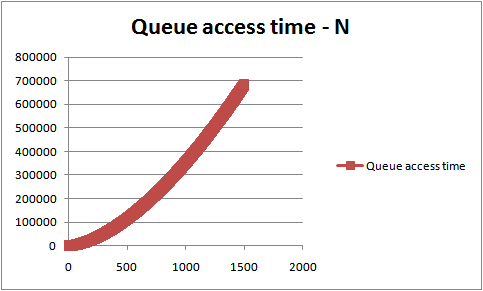
\includegraphics[scale=0.5]{img/big-O-1q.eps}
        \caption{Queue access count v.s. $n$.} \label{fig:big-O-1q}
       \end{center}
\end{figure}

The C program based on this algorithm takes only 0.016[s] to get the right answer
859963392. Which is 2500 times faster than the brute force solution.

%% Functional 1Q solution
Improvement 1 can also be considered in recursive way. Suppose $X$ is the infinity
series for all numbers which only contain factors of 2, 3, or 5. The following
formula shows an interesting relationship.

\be
  X = \{1\} \cup \{2x: \forall x \in X\} \cup \{3x: \forall x \in X \} \cup \{5x: \forall x \in X \}
\ee

Where we can define $\cup$ to a special form so that all elements are stored in order
as well as unique to each other. Suppose that $X=\{x_1, x_2, x_3...\}$, $Y=\{y_1, y_2, y_3, ...\}$, $X' = \{x_2, x_3, ...\}$ and $Y'=\{y_2, y_3, ...\}$. We have

\[
X \cup Y = \left \{
  \begin{array}{r@{\quad:\quad}l}
  X & Y = \phi \\
  Y & X = \phi \\
  \{ x_1, X' \cup Y \} & x_1 < y_1 \\
  \{ X' \cup Y' \} & x_1 = y_1 \\
  \{ y_1, X \cup Y' \} & x_1 > y_1
  \end{array}
\right.
\]

In a functional programming language such as Haskell, which supports 
lazy evaluation, The above infinity series functions can be translate
into the following program.

\lstset{language=Haskell}
\begin{lstlisting}
ns = 1:merge (map (*2) ns) (merge (map (*3) ns) (map (*5) ns))

merge [] l = l
merge l [] = l
merge (x:xs) (y:ys) | x <y = x : merge xs (y:ys)
                    | x ==y = x : merge xs ys
                    | otherwise = y : merge (x:xs) ys
\end{lstlisting}

By evaluate ns !! (n-1), we can get the 1500th number as
below.

\begin{verbatim}
>ns !! (1500-1)
859963392
\end{verbatim}

\subsection{Improvement 2}
Considering the above solution, although it is much faster than the brute-force one,
It still has some drawbacks. It produces many duplicated numbers and they are
finally dropped when examine the queue. Secondly, it does linear scan and insertion
to keep the order of all elements in the queue, which degrade the ENQUEUE operation
from $O(1)$ to $O(|Q|)$.

If we use three queues instead of using only one, we can improve the solution one
step ahead. Denote these queues as $Q_2$, $Q_3$, and $Q_5$, and we initialize
them as $Q_2=\{ 2 \}$, $Q_3 = \{ 3\}$ and $Q_5 = \{ 5 \}$. Each time we DEQUEUEed
the smallest one from $Q_2$, $Q_3$, and $Q_5$ as $x$. And do the following test:

\begin{itemize}
\item If $x$ comes from $Q_2$, we ENQUEUE $2x$, $3x$, and $5x$ back to 
$Q_2$, $Q_3$, and $Q_5$ respectively;
\item If $x$ comes from $Q_3$, we only need ENQUEUE $3x$ to $Q_3$, and $5x$ to $Q_5$;
We needn't ENQUEUE $2x$ to $Q_2$, because $2x$ have already existed in $Q_3$;
\item If $x$ comes from $Q_5$, we only need ENQUEUE $5x$ to $Q_5$; there is
no need to ENQUEUE $3x$, $5x$ to $Q_3$, $Q_5$ because they have already been
in the queues;
\end{itemize}

We repeatedly ENQUEUE the smallest one until we find the $n$-th element.

\begin{figure}[htbp]
       \begin{center}
       	  \includegraphics[scale=0.5]{img/q235-1.ps}
       	  \includegraphics[scale=0.5]{img/q235-2.ps}
       	  \includegraphics[scale=0.5]{img/q235-3.ps}
       	  \includegraphics[scale=0.5]{img/q235-4.ps}
        \caption{First 4 steps of constructing numbers with $Q_2$, $Q_3$, and $Q_5$. \newline
        1. Queues are initialized with 2, 3, 5 as the only element;\newline
        2. New elements 4, 6, and 10 are pushed back; \newline
        3. New elements 9, and 15, are pushed back; \newline
        4. New elements 8, 12, and 20 are pushed back; \newline
        5. New element 25 is pushed back.} \label{fig:q235}
       \end{center}
\end{figure}

The algorithm based on this idea is implemented as below.

\begin{algorithmic}[1]
\Function{Get-Number}{$n$}
  \If{$n = 1$}
    \State \Return $1$
  \Else
    \State $Q_2 \gets \{ 2 \}$
    \State $Q_3 \gets \{ 3 \}$
    \State $Q_5 \gets \{ 5 \}$
    \While{$n > 1$}
      \State $x \gets min($\Call{Head}{$Q_2$}, \Call{Head}{$Q_3$}, \Call{Head}{$Q_5$}$)$
      \If{$x = $ \Call{Head}{$Q_2$}}
        \State \Call{Dequeue}{$Q_2$}
        \State \Call{Enqueue}{$Q_2, 2x$}
        \State \Call{Enqueue}{$Q_3, 3x$}
        \State \Call{Enqueue}{$Q_5, 5x$}
      \ElsIf{$x=$ \Call{Head}{$Q_3$}}
        \State \Call{Dequeue}{$Q_3$}
        \State \Call{Enqueue}{$Q_3, 3x$}
        \State \Call{Enqueue}{$Q_5, 5x$}
      \Else
        \State \Call{Dequeue}{$Q_5$}
        \State \Call{Enqueue}{$Q_5, 5x$}
      \EndIf
      \State $n \gets n - 1$
    \EndWhile
    \State \Return $x$
  \EndIf
\EndFunction
\end{algorithmic}

This algorithm loops $n$ times, and within each loop, it extract one head
element from the three queues, which takes constant time. Then it appends
one to three new elements at the end of queues which bounds to constant time
too. So the total time of the algorithm bounds to $O(n)$. The C++ program
translated from this algorithm shown below takes less than 1 $\mu$s to 
produce the 1500th number, 859963392.

\lstset{language=C++}
\begin{lstlisting}
typedef unsigned long Integer;

Integer get_number(int n){
  if(n==1) 
    return 1;
  queue<Integer> Q2, Q3, Q5;
  Q2.push(2);
  Q3.push(3);
  Q5.push(5);
  Integer x;
  while(n-- > 1){
    x = min(min(Q2.front(), Q3.front()), Q5.front());
    if(x==Q2.front()){
      Q2.pop();
      Q2.push(x*2);
      Q3.push(x*3);
      Q5.push(x*5);
    }
    else if(x==Q3.front()){
      Q3.pop();
      Q3.push(x*3);
      Q5.push(x*5);
    }
    else{
      Q5.pop();
      Q5.push(x*5);
    }
  }
  return x;
}
\end{lstlisting}

This solution can be also implemented in Functional way. We define
a function $take(n)$, which will return the first $n$ numbers contains
only factor 2, 3, or 5.

\[
  take(n) = f(n, \{1\}, \{2\}, \{3\}, \{5\})
\]
Where
\[
 f(n, X, Q_2, Q_3, Q_5) = \left \{
  \begin{array}{r@{\quad:\quad}l}
  X & n = 1 \\
  f(n-1, X \cup \{x\}, Q_2', Q_3', Q_5') & otherwise
  \end{array}
\right.
\]

\[
 x = min(Q_{21}, Q_{31}, Q_{51})
\]
\[
 Q_2', Q_3', Q_5' = \left \{
 \begin{array}{r@{\quad:\quad}l}
 \{Q_{22}, Q_{23}, ...\} \cup \{2x\}, Q_3 \cup \{3x\}, Q_5 \cup \{5x\} & x = Q_{21} \\
 Q_2, \{Q_{32}, Q_{33}, ...\} \cup \{3x\}, Q5 \cup \{5x\} & x = Q_{31} \\
 Q_2, Q_3, \{Q_{52}, Q_{53}, ...\} \cup \{5x\} & x = Q_{51}
 \end{array}
 \right.
\]

And these functional definition can be realized in Haskell as the following.

\lstset{language=Haskell}
\begin{lstlisting}
ks 1 xs _ = xs
ks n xs (q2, q3, q5) = ks (n-1) (xs++[x]) update
    where 
      x = minimum $ map head [q2, q3, q5]
      update | x == head q2 = ((tail q2)++[x*2], q3++[x*3], q5++[x*5])
             | x == head q3 = (q2, (tail q3)++[x*3], q5++[x*5])
             | otherwise = (q2, q3, (tail q5)++[x*5])

takeN n = ks n [1] ([2], [3], [5])
\end{lstlisting} %$

Invoke `last takeN 1500' will generate the correct answer 859963392.

% ================================================================
%                 Short summary
% ================================================================
\section{Notes and short summary}
If review the 2 puzzles, we found in both cases, the brute-force solutions
are so weak. In the first problem, it's quite poor in dealing with
long ID list, while in the second problem, it doesn't work at all.

The first problem shows the power of algorithms, while the second 
problem tells why data structure is important. There are plenty
of interesting problems, which are hard to solve before computer
was invented. With the aid of computer and programming, we are able
to find the answer in a quite different way. Compare to what we 
learned in mathematics course in school, we haven't been taught the method 
like this. 

While there have been already a lot of wonderful books about
algorithms, data structures and math, however, few of them 
provide the comparison between the procedural solution and 
the functional solution. From the above discussion, it can be 
found that functional solution sometimes is very expressive 
and they are close to what we are familiar in mathematics.

This series of post focus on providing both imperative and functional
algorithms and data structures. Many functional data structures
can be referenced from Okasaki's book\cite{okasaki-book}. While
the imperative ones can be founded in classic text books \cite{CLRS}
or even in WIKIpedia.
Multiple
programming languages, including, C, C++, Python, Haskell, and
Scheme/Lisp will be used. In order to make it easy to read
by programmers with different background, pseudo code and mathematical
function are the regular descriptions of each post.

The author is NOT a native English speaker, the reason why 
this book is only available in English for the time being
is because the contents are still changing frequently. Any
feedback, comments, or criticizes are welcome.

\section{Structure of the contents}
In the following series of post, I'll first introduce about
elementary data structures before algorithms, because many
algorithms need knowledge of data structures as prerequisite.

The `hello world' data structure, binary search tree is the
first topic; Then we introduce how to solve the balance problem
of binary search tree. After that, I'll show other interesting
trees. Trie, Patricia, suffix trees are useful in text manipulation.
While B-trees are commonly used in file system and data base
implementation.

The second part of data structures is about heaps. We'll
provide a general Heap definition and introduce about binary
heaps by array and by explicit binary trees. Then we'll
extend to K-ary heaps including Binomial heaps, Fibonacci
heaps, and pairing heaps.

Array and queues are considered among the easiest data structures
typically, However, we'll show how difficult to implement 
them in the third part.

As the elementary sort algorithms, we'll introduce insertion
sort, quick sort, merge sort etc in both imperative way
and functional way.

The final part is about searching, besides the element
searching, we'll also show string matching algorithms
such as KMP.

All the posts are provided under GNU FDL (Free document
license), and programs are under GNU GPL.

% ================================================================
%                 Appendix
% ================================================================
\section{Appendix} \label{appendix}
%\appendix
All programs provided along with this article are free for
downloading. download position: 
  http://sites.google.com/site/algoxy/introduction

\begin{thebibliography}{99}

\bibitem{Bird-book}
Richard Bird. ``Pearls of functional algorithm design''. Cambridge University Press; 1 edition (November 1, 2010). ISBN-10: 0521513383

\bibitem{Bentley}
Jon Bentley. ``Programming Pearls(2nd Edition)''. Addison-Wesley Professional; 2 edition (October 7, 1999). ISBN-13: 978-0201657883

\bibitem{okasaki-book}
Chris Okasaki. ``Purely Functional Data Structures''. Cambridge university press, (July 1, 1999), ISBN-13: 978-0521663502

\bibitem{CLRS}
Thomas H. Cormen, Charles E. Leiserson, Ronald L. Rivest and Clifford Stein. ``Introduction to Algorithms, Second Edition''. The MIT Press, 2001. ISBN: 0262032937.

\end{thebibliography}

\ifx\wholebook\relax \else
\end{document}
\fi


\part{Trees}
\ifx\wholebook\relax \else
% ------------------------ 

\documentclass{article}
%------------------- Other types of document example ------------------------
%
%\documentclass[twocolumn]{IEEEtran-new}
%\documentclass[12pt,twoside,draft]{IEEEtran}
%\documentstyle[9pt,twocolumn,technote,twoside]{IEEEtran}
%
%-----------------------------------------------------------------------------
%%
% loading packages
%
\newif\ifpdf
\ifx\pdfoutput\undefined % We're not running pdftex
  \pdffalse
\else
  \pdftrue
\fi
%
%
\ifpdf
  \RequirePackage[pdftex,%
            CJKbookmarks,%
       bookmarksnumbered,%
              colorlinks,%
          linkcolor=blue,%
              hyperindex,%
        plainpages=false,%
       pdfstartview=FitH]{hyperref}
\else
  \RequirePackage[dvipdfm,%
             CJKbookmarks,%
        bookmarksnumbered,%
               colorlinks,%
           linkcolor=blue,%
               hyperindex,%
         plainpages=false,%
        pdfstartview=FitH]{hyperref}
  \AtBeginDvi{\special{pdf:tounicode GBK-EUC-UCS2}} % GBK -> Unicode
\fi
\usepackage{hyperref}

% other packages
%-----------------------------------------------------------------------------
\usepackage{graphicx, color}
\usepackage{CJK}
%
% for programming 
%
\usepackage{verbatim}
\usepackage{listings}


\lstdefinelanguage{Smalltalk}{
  morekeywords={self,super,true,false,nil,thisContext}, % This is overkill
  morestring=[d]',
  morecomment=[s]{"}{"},
  alsoletter={\#:},
  escapechar={!},
  literate=
    {BANG}{!}1
    {UNDERSCORE}{\_}1
    {\\st}{Smalltalk}9 % convenience -- in case \st occurs in code
    % {'}{{\textquotesingle}}1 % replaced by upquote=true in \lstset
    {_}{{$\leftarrow$}}1
    {>>>}{{\sep}}1
    {^}{{$\uparrow$}}1
    {~}{{$\sim$}}1
    {-}{{\sf -\hspace{-0.13em}-}}1  % the goal is to make - the same width as +
    %{+}{\raisebox{0.08ex}{+}}1		% and to raise + off the baseline to match -
    {-->}{{\quad$\longrightarrow$\quad}}3
	, % Don't forget the comma at the end!
  tabsize=2
}[keywords,comments,strings]

\lstloadlanguages{C++, Lisp, Haskell, Python, Smalltalk}

% ======================================================================

\def\BibTeX{{\rm B\kern-.05em{\sc i\kern-.025em b}\kern-.08em
    T\kern-.1667em\lower.7ex\hbox{E}\kern-.125emX}}

\newtheorem{theorem}{Theorem}

%
% mathematics
%
\newcommand{\be}{\begin{equation}}
\newcommand{\ee}{\end{equation}}
\newcommand{\bmat}[1]{\left( \begin{array}{#1} }
\newcommand{\emat}{\end{array} \right) }
\newcommand{\VEC}[1]{\mbox{\boldmath $#1$}}

% numbered equation array
\newcommand{\bea}{\begin{eqnarray}}
\newcommand{\eea}{\end{eqnarray}}

% equation array not numbered
\newcommand{\bean}{\begin{eqnarray*}}
\newcommand{\eean}{\end{eqnarray*}}

\RequirePackage{CJK,CJKnumb,CJKulem,CJKpunct}
% we use CJK as default environment
\AtBeginDocument{\begin{CJK*}{GBK}{song}\CJKtilde\CJKindent\CJKcaption{GB}}
\AtEndDocument{\clearpage\end{CJK*}}

%
% loading packages
%

\RequirePackage{ifpdf}

%
%
\ifpdf
  \RequirePackage[pdftex,%
       bookmarksnumbered,%
              colorlinks,%
          linkcolor=blue,%
              hyperindex,%
        plainpages=false,%
       pdfstartview=FitH]{hyperref}
\else
  \RequirePackage[dvipdfm,%
        bookmarksnumbered,%
               colorlinks,%
           linkcolor=blue,%
               hyperindex,%
         plainpages=false,%
        pdfstartview=FitH]{hyperref}
\fi
\usepackage{hyperref}

% other packages
%--------------------------------------------------------------------------
\usepackage{graphicx, color}
\usepackage{subfig}

\usepackage{amsmath, amsthm, amssymb} % for math
\usepackage{exercise} % for exercise

%
% for programming 
%
\usepackage{verbatim}
\usepackage{listings}
%\usepackage{algorithmic} %old version; we can use algorithmicx instead
\usepackage{algorithm} 
\usepackage[noend]{algpseudocode} %for pseudo code, include algorithmicsx automatically
\usepackage{makeidx} % for index support


\lstdefinelanguage{Smalltalk}{
  morekeywords={self,super,true,false,nil,thisContext}, % This is overkill
  morestring=[d]',
  morecomment=[s]{"}{"},
  alsoletter={\#:},
  escapechar={!},
  literate=
    {BANG}{!}1
    {UNDERSCORE}{\_}1
    {\\st}{Smalltalk}9 % convenience -- in case \st occurs in code
    % {'}{{\textquotesingle}}1 % replaced by upquote=true in \lstset
    {_}{{$\leftarrow$}}1
    {>>>}{{\sep}}1
    {^}{{$\uparrow$}}1
    {~}{{$\sim$}}1
    {-}{{\sf -\hspace{-0.13em}-}}1  % the goal is to make - the same width as +
    %{+}{\raisebox{0.08ex}{+}}1		% and to raise + off the baseline to match -
    {-->}{{\quad$\longrightarrow$\quad}}3
	, % Don't forget the comma at the end!
  tabsize=2
}[keywords,comments,strings]

\lstloadlanguages{C++, Lisp, Haskell, Python, Smalltalk}

% ======================================================================

\def\BibTeX{{\rm B\kern-.05em{\sc i\kern-.025em b}\kern-.08em
    T\kern-.1667em\lower.7ex\hbox{E}\kern-.125emX}}

%
% mathematics
%
\newcommand{\be}{\begin{equation}}
\newcommand{\ee}{\end{equation}}
\newcommand{\bmat}[1]{\left( \begin{array}{#1} }
\newcommand{\emat}{\end{array} \right) }
\newcommand{\VEC}[1]{\mbox{\boldmath $#1$}}

% numbered equation array
\newcommand{\bea}{\begin{eqnarray}}
\newcommand{\eea}{\end{eqnarray}}

% equation array not numbered
\newcommand{\bean}{\begin{eqnarray*}}
\newcommand{\eean}{\end{eqnarray*}}

\newtheorem{theorem}{Theorem}[section]
\newtheorem{lemma}[theorem]{Lemma}
\newtheorem{proposition}[theorem]{Proposition}
\newtheorem{corollary}[theorem]{Corollary}


\setcounter{page}{1}

\begin{document}

\fi
%--------------------------

% ================================================================
%                 COVER PAGE
% ================================================================

\title{Binary search tree, the `hello world' data structure}

\author{Larry~LIU~Xinyu
\thanks{{\bfseries Larry LIU Xinyu } \newline
  Email: liuxinyu95@gmail.com \newline}
  }

\markboth{Binary search tree}{AlgoXY}

\maketitle

\ifx\wholebook\relax
\chapter{Binary search tree, the `hello world' data structure}
\numberwithin{Exercise}{chapter}
\fi

% ================================================================
%                 Introduction
% ================================================================
\section{Introduction}
\label{introduction} \index{binary search tree}

It's typically considered that Arrays or Lists are the `hello world' data structure.
However, we'll see they are not so easy to implement actually. In some procedural 
settings, Arrays are the elementary representation, and it is possible to realize
linked list by array (section 10.3 in \cite{CLRS}); While in some functional settings,
Linked list are the elementary bricks to build arrays and other data structures.

Considering these factors, we start with Binary Search Tree (or BST) as the `hello world'
data structure. Jon Bentley mentioned an interesting problem in `programming pearls'
\cite{Bentley}. The problem is about to count the number of times each word occurs
in a big text. And the solution is something like the below C++ code.\index{word counter}

\lstset{language=C++}
\begin{lstlisting}
int main(int, char** ){
  map<string, int> dict;
  string s;
  while(cin>>s)
    ++dict[s];
  map<string, int>::iterator it=dict.begin();
  for(; it!=dict.end(); ++it)
    cout<<it->first<<": "<<it->second<<"\n";
}
\end{lstlisting}

And we can run it to produce the word counting result as the following
\footnote{This is not UNIX unique command, in Windows OS, it can be achieved
by: $type \quad bbe.txt | wordcount.exe > wc.txt$}.

\begin{verbatim}
$ g++ wordcount.cpp -o wordcount
$ cat bbe.txt | ./wordcount > wc.txt
\end{verbatim}

The map provided in standard template library is a kind of balanced binary search tree
with augmented data. Here we use the word in the text as the key and the number of 
occurrence as the augmented data. This program is fast, and it reflects the power of
binary search tree. We'll introduce how to implement BST in this post and show how
to solve the balancing problem in later post.

Before we dive into binary search tree. Let's first introduce about
the more general binary tree.

The concept of Binary tree is a recursive definition. Binary search tree is just a special 
type of binary tree. The Binary tree is typically defined as the following.
\index{binary tree}

A binary tree is 
\begin{itemize}
\item either an empty node;
\item or a node contains 3 parts, a value, a left child which is a binary tree and a 
right child which is also a binary tree.
\end{itemize}

Figure \ref{fig:binary-tree-example} shows this concept and an example binary tree.

\begin{figure}[htbp]
  \centering
  \subfloat[Concept of binary tree]{\includegraphics[scale=0.5]{img/lvr.ps}} \\
  \subfloat[An example binary tree]{\includegraphics[scale=0.5]{img/btexample.ps}}
  \caption{Binary tree concept and an example.} 
  \label{fig:binary-tree-example}
\end{figure}

A binary search tree is a binary tree which satisfies the below criteria.
for each node in binary search tree,
\begin{itemize}
\item all the values in left child tree are less than the value of of this node;
\item the value of this node is less than any values in its right child tree.
\end{itemize}

Figure \ref{fig:bst-example} shows an example of binary search tree. Compare with
Figure \ref{fig:binary-tree-example} we can see the difference about the key 
ordering between them.

\begin{figure}[htbp]
       \begin{center}
        \includegraphics[scale=0.5]{img/bst-1.ps}
        \caption{A Binary search tree example.} \label{fig:bst-example}
       \end{center}
\end{figure}


% ================================================================
% Data layout
% ================================================================
\section{Data Layout}
\index{binary search tree!data layout}

Based on the recursive definition of binary search tree, we can draw the 
data layout in procedural setting with pointer supported as in figure
\ref{fig:node-layout-parent}.

%\begin{figure}[htbp]
%       \begin{center}
%        \includegraphics[scale=0.8]{img/node-layout.ps}
%        \caption{Node layout.} \label{fig:node-layout}
%       \end{center}
%\end{figure}

The node contains a field of key, which can be augmented with satellite
data; a field contains a pointer to the left child and a field point to
the right child. In order to back-track an ancestor easily, a parent
field can be provided as well. 
%Figure \ref{fig:node-layout-parent} shows the layout with parent field.

\begin{figure}[htbp]
       \begin{center}
        \includegraphics[scale=0.8]{img/node-layout-parent.ps}
        \caption{Layout of nodes with parent field.} \label{fig:node-layout-parent}
       \end{center}
\end{figure}

In this post, we'll ignore the satellite data for simple illustration purpose.
Based on this layout, the node of binary search tree can be defined in a procedural
language, such as C++ as the following.

\lstset{language=C++}
\begin{lstlisting}
template<class T>
struct node{
  node(T x):key(x), left(0), right(0), parent(0){}
  ~node(){ 
    delete left;
    delete right;
  }

  node* left; 
  node* right;
  node* parent; //parent is optional, it's helpful for succ/pred
  T key;
};
\end{lstlisting}

There is another setting, for instance in Scheme/Lisp languages, the elementary
data structure is linked-list. Figure \ref{fig:lisp-layout} shows how a binary
search tree node can be built on top of linked-list.

\begin{figure}[htbp]
       \begin{center}
        \includegraphics[scale=0.8]{img/lisp-layout.ps}
        \caption{Binary search tree node layout on top of linked list. Where `left...' and 'right ...' are either empty or binary search tree node composed in the same way.} \label{fig:lisp-layout}
       \end{center}
\end{figure}

Because in pure functional setting, It's hard to use pointer for back tracking
the ancestors, (and typically, there is no need to do back tracking, since
we can provide top-down solution in recursive way) there is not `parent' field
in such layout.

For simplified reason, we'll skip the detailed layout in the future, and only 
focus on the logic layout of data structures. For example, below is the definition
of binary search tree node in Haskell.

\lstset{language=Haskell}
\begin{lstlisting}
data Tree a = Empty 
            | Node (Tree a) a (Tree a)
\end{lstlisting}

% ================================================================
% Insert
% ================================================================
\section{Insertion}
\index{binary search tree!insertion}

To insert a key $k$ (may be along with a value in practice) to a binary search tree $T$, we can follow a quite straight forward way.

\begin{itemize}
\item If the tree is empty, then construct a leave node with key=$k$;
\item If $k$ is less than the key of root node, insert it to the left child;
\item If $k$ is greater than the key of root, insert it to the right child;
\end{itemize}

There is an exceptional case that if $k$ is equal to the key of root, it means it has already existed, we can either overwrite the data, or just do nothing.
For simple reason, this case is skipped in this post.

This algorithm is described recursively. It is so simple that is why we 
consider binary search tree is `hello world' data structure. Formally, 
the algorithm can be represented with a recursive function.

\be
insert(T, k) = \left \{
  \begin{array}
  {r@{\quad:\quad}l}
  node(\phi, k, \phi) & T = \phi \\
  node(insert(L, k), Key, R) & k < Key \\
  node(L, Key, insert(R, k)) & otherwise
  \end{array}
\right.
\ee 

Where 
\[
  \begin{array}{l}
  L = left(T) \\
  R = right(T) \\
  Key = key(T)
  \end{array}
\]

The node function creates a new node with given left sub-tree,
a key and a right sub-tree as parameters. $\phi$ means NIL or Empty.
function $left$, $right$ and $key$ are access functions which can 
get the left sub-tree, right sub-tree and the key of a node.

Translate the above functions directly to Haskell yields the following
program.

\lstset{language=Haskell}
\begin{lstlisting}
insert::(Ord a) => Tree a -> a -> Tree a
insert Empty k = Node Empty k Empty
insert (Node l x r) k | k < x = Node (insert l k) x r
                      | otherwise = Node l x (insert r k)
\end{lstlisting}

This program utilized the pattern matching features provided by the 
language. However, even in functional settings without this feature,
for instance, Scheme/Lisp, the program is still expressive.

\lstset{language=lisp}
\begin{lstlisting}
(define (insert tree x)
  (cond ((null? tree) (list '() x '()))
	((< x (key tree))
	 (make-tree (insert (left tree) x)
		    (key tree)
		    (right tree)))
	((> x (key tree))
	 (make-tree (left tree)
		    (key tree)
		    (insert (right tree) x)))))
\end{lstlisting}

It is possible to turn the algorithm completely into imperative way
without recursion. 

\begin{algorithmic}[1]
\Function{Insert}{$T, k$}
  \State $root \gets T$
  \State $x \gets$ \Call{Create-Leaf}{$k$}
  \State $parent \gets NIL$
  \While{$T \neq NIL$}
    \State $parent \gets T$
    \If{$k <$ \Call{Key}{$T$}}
      \State $T \gets $ \Call{Left}{$T$}
    \Else
      \State $T \gets $ \Call{Right}{$T$}
    \EndIf
  \EndWhile
  \State \Call{Parent}{$x$} $\gets parent$
  \If{$parent = NIL$} \Comment{tree $T$ is empty}
    \State \Return $x$
  \ElsIf{$k <$ \Call{Key}{$parent$}}
    \State \Call{Left}{$parent$} $\gets x$
  \Else
    \State \Call{Right}{$parent$} $\gets x$
  \EndIf
  \State \Return $root$
\EndFunction
\Statex
\Function{Create-Leaf}{k}
  \State $x \gets $ \Call{Empty-Node}{}
  \State \Call{Key}{$x$} $ \gets k$
  \State \Call{Left}{$x$} $ \gets NIL$
  \State \Call{Right}{$x$} $ \gets NIL$
  \State \Call{Parent}{$x$} $ \gets NIL$
  \State \Return $x$
\EndFunction
\end{algorithmic}

Compare with the functional algorithm, it is obviously that this one
is more complex although it is fast and can handle very deep tree. A 
complete C++ program and a python program are available along with this
post for reference.

\section{Traversing}
\index{binary search tree!traverse}

Traversing means visiting every element one by one in a binary 
search tree. There are 3 ways to traverse a binary tree, pre-order tree walk, 
in-order tree walk, and post-order tree walk. The names of these
traversing methods highlight the order of when we visit the root
of a binary search tree.

Since there are three parts in a tree, as left child, the root, which
contains the key and satellite data, and the right child. If we denote
them as $(left, current, right)$, the three traversing methods are defined 
as the following.

\begin{itemize}
\item pre-order traverse, visit $current$, then $left$, finally $right$;
\item in-order traverse, visit $left$ , then $current$, finally $right$;
\item post-order traverse, visit $left$, then $right$, finally $current$.
\end{itemize}

\index{pre-order traverse} \index{in-order traverse} \index{post-order traverse}

Note that each visiting operation is recursive. And we see the order
of visiting $current$ determines the name of the traversing method.

For the binary search tree shown in figure \ref{fig:bst-example}, below
are the three different traversing results.

\begin{itemize}
\item pre-order traverse result: 4, 3, 1, 2, 8, 7, 16, 10, 9, 14;
\item in-order traverse result: 1, 2, 3, 4, 7, 8, 9, 10, 14, 16;
\item post-order traverse result: 2, 1, 3, 7, 9, 14, 10, 16, 8, 4;
\end{itemize}

It can be found that the in-order walk of a binary search tree outputs
the elements in increase order, which is particularly helpful. The definition
of binary search tree ensures this interesting property, while the
proof of this fact is left as an exercise of this post.

In-order tree walk algorithm can be described as the following:
\begin{itemize}
\item If the tree is empty, just return;
\item traverse the left child by in-order walk, then access the key, 
finally traverse the right child by in-order walk.
\end{itemize}

Translate the above description yields a generic map function

\be
map(f, T) = \left \{
  \begin{array}
  {r@{\quad:\quad}l}
  \phi & T = \phi \\
  node(l', k', r') & otherwise
  \end{array}
\right .
\ee

where

\[
 \begin{array}{l}
 l' = map(f, left(T)) \\
 r' = map(f, right(T)) \\
 k' = f(key(T))
 \end{array}
\]

If we only need access the key without create the transformed tree,
we can realize this algorithm in procedural way lie the below C++
program.

\lstset{language=C++}
\begin{lstlisting}
template<class T, class F>
void in_order_walk(node<T>* t, F f){
  if(t){
    in_order_walk(t->left, f);
    f(t->value);
    in_order_walk(t->right, f);
  }
}
\end{lstlisting}

The function takes a parameter f, it can be a real function, or a function
object, this program will apply f to the node by in-order tree walk.

We can simplified this algorithm one more step to define a function 
which turns a binary search tree to a sorted list by in-order traversing.

\be
toList(T) = \left \{
  \begin{array}
  {r@{\quad:\quad}l}
  \phi & T = \phi \\
  toList(left(T)) \cup \{ key(T) \} \cup toList(right(T)) & otherwise
  \end{array}
\right .
\ee

Below is the Haskell program based on this definition.

\lstset{language=Haskell}
\begin{lstlisting}
toList::(Ord a)=>Tree a -> [a]
toList Empty = []
toList (Node l x r) = toList l ++ [x] ++ toList r
\end{lstlisting}

This provides us a method to sort a list of elements. We can first
build a binary search tree from the list, then output the tree
by in-order traversing. This method is called as `tree sort'.
Let's denote the list $X = \{x_1, x_2, x_3, ..., x_n\}$.

\be
  sort(X) = toList(fromList(X))
\ee

And we can write it in function composition form.

\[
  sort = toList . fromList
\]

Where function $fromList$ repeatedly insert every element to a 
binary search tree.

\be
  fromList(X)= foldL(insert, \phi, X)
\ee

It can also be written in partial application form like below.

\[
  fromList = foldL \quad insert \quad \phi
\]

For the readers who are not familiar with folding from left, this function
can also be defined recursively as the following.

\[
fromList(X) = \left \{
  \begin{array}
  {r@{\quad:\quad}l}
  \phi & X = \phi \\
  insert(fromList(\{x_2, x_3, ..., x_n\}), x_1) & otherwise
  \end{array}
\right .
\]

We'll intense use folding function as well as the function composition
and partial evaluation in the future, please refer to appendix of this
book or \cite{wiki-fold}
\cite{func-composition} and \cite{curry} for more information.

\begin{Exercise}

\begin{itemize}
\item Given the in-order traverse result and pre-order traverse result, 
can you re-construct the tree from these result and figure out the 
post-order traversing result?

Pre-order result: 1, 2, 4, 3, 5, 6;
In-order result: 4, 2, 1, 5, 3, 6;
Post-order result: ?
\index{tree reconstruction}

\item Write a program in your favorite language to re-construct
the binary tree from pre-order result and in-order result.

\item Prove why in-order walk output the elements stored in a binary
search tree in increase order?

\item Can you analyze the performance of tree sort with big-O notation?
\end{itemize}
\end{Exercise}

% ================================================================
% Querying a binary search tree
% ================================================================
\section{Querying a binary search tree}
\index{binary search tree!search}
\index{binary search tree!looking up}

There are three types of querying for binary search tree, searching
a key in the tree, find the minimum or maximum element in the tree,
and find the predecessor or successor of an element in the tree.

\subsection{Looking up}
According to the definition of binary search tree, search
a key in a tree can be realized as the following.

\begin{itemize}
\item If the tree is empty, the searching fails;
\item If the key of the root is equal to the value to be found, the
search succeed. The root is returned as the result;
\item If the value is less than the key of the root, search in the left
child.
\item Else, which means that the value is greater than the key of the 
root, search in the right child.
\end{itemize}

This algorithm can be described with a recursive function as below.

\be
lookup(T, x) = \left \{
  \begin{array}
  {r@{\quad:\quad}l}
  \phi & T = \phi \\
  T & key(T) = x \\
  lookup(left(T), x) & x < key(T) \\
  lookup(right(T), x) & otherwise
  \end{array}
\right .
\ee

In the real application, we may return the satellite data instead of the
node as the search result. This algorithm is simple and straightforward.
Here is a translation of Haskell program.

\lstset{language=Haskell}
\begin{lstlisting}
lookup::(Ord a)=> Tree a -> a -> Tree a
lookup Empty _ = Empty
lookup t@(Node l k r) x | k == x = t
                        | x < k = lookup l x
                        | otherwise = lookup r x
\end{lstlisting}

If the binary search tree is well balanced, which means that almost
all nodes have both non-NIL left child and right child, for $N$ elements,
the search algorithm takes $O(\lg N)$ time to perform. This is not
formal definition of balance. We'll show it in later post about red-black-tree.
If the tree is poor balanced, the worst case takes $O(N)$ time to 
search for a key. If we denote the height of the tree as $h$, we can
uniform the performance of the algorithm as $O(h)$.

The search algorithm can also be realized without using recursion in 
a procedural manner.

\begin{algorithmic}[1]
\Function{Search}{$T, x$}
  \While{$T \neq NIL \wedge$ \Call{Key}{$T$} $ \neq x$}
    \If{$x <$ \Call{Key}{$T$}}
      \State $T \gets $ \Call{Left}{$T$}
    \Else
      \State $T \gets $ \Call{Right}{$T$}
    \EndIf
  \EndWhile
  \State \Return $T$
\EndFunction
\end{algorithmic}

Below is the C++ program based on this algorithm.

\lstset{language=C++}
\begin{lstlisting}
template<class T>
node<T>* search(node<T>* t, T x){
  while(t && t->key!=x){
    if(x < t->key) t=t->left;
    else t=t->right;
  }
  return t;
}
\end{lstlisting}

\subsection{Minimum and maximum}
\index{binary search tree!min/max}

Minimum and maximum can be implemented from the property of binary search
tree, less keys are always in left child, and greater keys are in right.

For minimum, we can continue traverse the left sub tree until it is empty.
While for maximum, we traverse the right.

\be
min(T) = \left \{
  \begin{array}
  {r@{\quad:\quad}l}
  key(T) & left(T) = \phi \\
  min(left(T)) & otherwise
  \end{array}
\right .
\ee

\be
max(T) = \left \{
  \begin{array}
  {r@{\quad:\quad}l}
  key(T) & right(T) = \phi \\
  max(right(T)) & otherwise
  \end{array}
\right .
\ee

Both function bound to $O(h)$ time, where $h$ is the height of the tree.
For the balanced binary search tree, $min$/$max$ are bound to $O(\lg N)$ time,
while they are $O(N)$ in the worst cases.

We skip translating them to programs, It's also possible to implement them 
in pure procedural way without using recursion.

\subsection{Successor and predecessor}
\index{binary search tree!succ/pred}

The last kind of querying, to find the successor or predecessor of an element
is useful when a tree is treated as a generic container and traversed by 
using iterator. It will be relative easier to implement if parent of
a node can be accessed directly. 

It seems that the functional solution is hard to be found, because there
is no pointer like field linking to the parent node. One solution is
to left `breadcrumbs' when we visit the tree, and use these information
to back-track or even re-construct the whole tree. Such data structure,
that contains both the tree and `breadcrumbs' is called zipper.
please refer to \cite{zipper-hbook} for details.

However, If we consider
the original purpose of providing $succ$/$pred$ function, `to traverse all the
binary search tree elements one by one` as a generic container, we realize
that they don't make significant sense in functional settings because 
we can traverse the tree in increase order by $mapT$ function we defined 
previously.

We'll meet many problems in this series of post that they are only valid
in imperative settings, and they are not meaningful problems in functional
settings at all. One good example is how to delete an element in 
red-black-tree\cite{okasaki-blog}.

In this section, we'll only present the imperative algorithm for finding
the successor and predecessor in a binary search tree.

When finding the successor of element $x$, which is the smallest one $y$
that satisfies $y > x$, there are two cases. If the node with value $x$
has non-NIL right child, the minimum element in right child is the answer;
For example, in Figure \ref{fig:bst-example}, in order to find the successor
of 8, we search it's right sub tree for the minimum one, which yields 9
as the result. While if node $x$ don't have right child, we need 
back-track to find the closest ancestors whose left child is also ancestor
of $x$. In Figure \ref{fig:bst-example}, since 2 don't have right sub tree,
we go back to its parent 1. However, node 1 don't have left child, so we
go back again and reach to node 3, the left child of 3, is also ancestor
of 2, thus, 3 is the successor of node 2.

Based on this description, the algorithm can be given as the following.

\begin{algorithmic}[1]
\Function{Succ}{$x$}
  \If{\Call{Right}{$x$} $\neq NIL$}
    \State \Return \textproc{Min}(\Call{Right}{$x$})
  \Else
    \State $p \gets $ \Call{Parent}{$x$}
    \While{$p \neq NIL$ and $x =$ \Call{Right}{$p$}}
      \State $x \gets p$
      \State $p \gets $ \Call{Parent}{$p$}
    \EndWhile
    \State \Return $p$
  \EndIf
\EndFunction
\end{algorithmic}

The predecessor case is quite similar to the successor algorithm, they
are symmetrical to each other. 

\begin{algorithmic}[1]
\Function{Pred}{$x$}
  \If{\Call{Left}{$x$} $\neq NIL$}
    \State \Return \textproc{Max}(\Call{Left}{$x$})
  \Else
    \State $p \gets $ \Call{Parent}{$x$}
    \While{$p \neq NIL$ and $x =$ \Call{Left}{$p$}}
      \State $x \gets p$
      \State $p \gets $ \Call{Parent}{$p$}
    \EndWhile
    \State \Return $p$
  \EndIf
\EndFunction
\end{algorithmic}

Below are the Python programs based on these algorithms. They are changed
a bit in while loop conditions.

\lstset{language=Python}
\begin{lstlisting}
def succ(x):
    if x.right is not None: return tree_min(x.right)
    p = x.parent
    while p is not None and p.left != x:
        x = p
        p = p.parent
    return p

def pred(x):
    if x.left is not None: return tree_max(x.left)
    p = x.parent
    while p is not None and p.right != x:
        x = p
        p = p.parent
    return p
\end{lstlisting}

\begin{Exercise}

\begin{itemize}
\item Can you figure out how to iterate a tree as a generic container
by using $pred()$/$succ()$? What's the performance of such traversing
process in terms of big-O?

\item A reader discussed about traversing all elements inside a 
range $[a, b]$. In C++, the algorithm looks like the below code:

$\mathbf{for\_each} (m.lower\_bound(12), m.upper\_bound(26), f);$

Can you provide the purely function solution for this problem?
\index{range traverse}
\end{itemize}

\end{Exercise}

% ================================================================
%                 Deletion
% ================================================================
\section{Deletion}
\index{binary search tree!delete}
Deletion is another `imperative only' topic for binary search tree.
This is because deletion mutate the tree, while in purely functional
settings, we don't modify the tree after building it in most 
application.

However, One method of deleting element from binary search
tree in purely functional way is shown in this section. It's actually
reconstructing the tree but not modifying the tree.

Deletion is the most complex operation for binary search tree. 
this is because we must keep the BST property, that for any node,
all keys in left sub tree are less than the key of this node, and
they are all less than any keys in right sub tree. Deleting a node
can break this property.

In this post, different with the algorithm described in \cite{CLRS}, 
A simpler one from SGI STL implementation is used.\cite{sgi-stl}

To delete a node $x$ from a tree.
\begin{itemize}
\item If $x$ has no child or only one child, splice x out;
\item Otherwise ($x$ has two children), use minimum element of its right sub tree to replace $x$, and splice the original minimum element out.
\end{itemize}

The simplicity comes from the truth that, the minimum element is stored
in a node in the right sub tree, which can't have two non-NIL children.
It ends up in the trivial case, the the node can be directly splice
out from the tree.

Figure \ref{fig:del-leaf}, \ref{fig:del-1child}, and \ref{fig:del-branch}
illustrate these different cases when deleting a node from the tree.

\begin{figure}[htbp]
       \begin{center}
	\includegraphics[scale=0.5]{img/del-leaf.ps}
        \caption{$x$ can be spliced out.} \label{fig:del-leaf}
       \end{center}
\end{figure}

\begin{figure}[htbp]
        \centering
        \subfloat[Before delete $x$]{\includegraphics[scale=0.5]{img/del-lc-before.ps}} 
        \subfloat[After delete $x$]{\includegraphics[scale=0.5]{img/del-lc-after.ps}} \\
        $x$ is spliced out, and replaced by its left child. \\
        \subfloat[Before delete $x$]{\includegraphics[scale=0.5]{img/del-rc-before.ps}} 
        \subfloat[Before delete $x$]{\includegraphics[scale=0.5]{img/del-rc-after.ps}} \\
        $x$ is spliced out, and replaced by its right child.
        \caption{Delete a node which has only one non-NIL child.} 
        \label{fig:del-1child}
\end{figure}

\begin{figure}[htbp]
        \centering
        \subfloat[Before delete $x$]{\includegraphics[scale=0.5]{img/del-branch-before.ps}}
        \subfloat[After delete $x$]{ \includegraphics[scale=0.5]{img/del-branch-after.ps}} \\
        $x$ is replaced by splicing the minimum element from its right child.
        \caption{Delete a node which has both children.} 
        \label{fig:del-branch}
\end{figure}

Based on this idea, the deletion can be defined as the below function.

\be
delete(T, x) = \left \{
  \begin{array}
  {r@{\quad:\quad}l}
  \phi & T = \phi \\
  node(delete(L, x), K, R) & x < K \\
  node(L, K, delete(R, x)) & x > K \\
  R & x = K \wedge L = \phi \\
  L & x = K \wedge R = \phi \\
  node(L, y, delete(R, y)) & otherwise
  \end{array}
\right .
\ee

Where
\[
\begin{array}{l}
L = left(T) \\
R = right(T) \\
K = key(T) \\
y = min(R)
\end{array}
\]

Translating the function to Haskell yields the below program.

\lstset{language=Haskell}
\begin{lstlisting}
delete::(Ord a)=> Tree a -> a -> Tree a
delete Empty _ = Empty
delete (Node l k r) x | x < k = (Node (delete l x) k r)
                      | x > k = (Node l k (delete r x))
                      -- x == k
                      | isEmpty l = r
                      | isEmpty r = l
                      | otherwise = (Node l k' (delete r k')) 
                          where k' = min r
\end{lstlisting}

Function `isEmpty' is used to test if a tree is empty ($\phi$).
Note that the algorithm first performs search to locate the node
where the element need be deleted, after that it execute the 
deletion. This algorithm takes $O(h)$ time where $h$ is the height
of the tree.

It's also possible to pass the node but not the element to the 
algorithm for deletion. Thus the searching is no more needed.

The imperative algorithm is more complex because it need set the 
parent properly. The function will return the root of the result tree.

\begin{algorithmic}[1]
\Function{Delete}{$T, x$}
  \State $root \gets T$
  \State $x' \gets x$ \Comment{save $x$}
  \State $parent \gets $ \Call{Parent}{$x$}
  \If{\Call{Left}{$x$} $= NIL$}
    \State $x \gets $ \Call{Right}{$x$}
  \ElsIf{\Call{Right}{$x$} $= NIL$}
    \State $x \gets $ \Call{Left}{$x$}
  \Else
    \Comment{both children are non-NIL}
    \State  $y \gets $ \textproc{Min}(\Call{Right}{$x$})
    \State \Call{Key}{$x$} $\gets$ \Call{Key}{$y$}
    \State Copy other satellite data from $y$ to $x$
    \If{\Call{Parent}{$y$} $\neq x$}
      \Comment{$y$ hasn't left sub tree}
      \State \textproc{Left}(\Call{Parent}{$y$}) $\gets$ \Call{Right}{$y$}
    \Else
      \Comment{$y$ is the root of right child of $x$}
      \State \Call{Right}{$x$} $\gets$ \Call{Right}{$y$}
    \EndIf
    \State Remove $y$
    \State \Return $root$
  \EndIf
  \If{$x \neq NIL$}
    \State \Call{Parent}{$x$} $\gets parent$ 
  \EndIf
  \If{$parent = NIL$}
    \Comment{We are removing the root of the tree}
    \State $root \gets x$
  \Else
    \If{\Call{Left}{$parent$} $= x'$}
      \State \Call{Left}{$parent$} $\gets x$
    \Else
      \State \Call{Right}{$parent$} $\gets x$
    \EndIf
  \EndIf
  \State Remove $x'$
  \State \Return $root$
\EndFunction
\end{algorithmic}

Here we assume the node to be deleted is not empty (otherwise we can 
simply returns the original tree). In other cases, it will first record 
the root of the tree, create copy pointers to $x$, and its parent.

If either of the children is empty, the algorithm just splice $x$ out. 
If it has two non-NIL children, we first located the minimum of right 
child, replace the key of $x$ to $y$'s, copy the satellite data as
well, then splice $y$ out. Note that there is a special case that $y$
is the root node of $x$'s left sub tree.

Finally we need reset the stored parent if the original $x$ has only 
one non-NIL child. 
If the parent pointer we copied before is empty, it
means that we are deleting the root node, so we need return the new root. After
the parent is set properly, we finally remove the old x from memory.

The relative Python program for deleting algorithm is given as below.
Because Python provides GC, we needn't explicitly remove the node
from the memory.

\lstset{language=Python}
\begin{lstlisting}
def tree_delete(t, x):
    if x is None: 
        return t
    [root, old_x, parent] = [t, x, x.parent]
    if x.left is None:
        x = x.right
    elif x.right is None:
        x = x.left
    else:
        y = tree_min(x.right)
        x.key = y.key
        if y.parent != x:
            y.parent.left = y.right
        else:
            x.right = y.right
        return root
    if x is not None:
        x.parent = parent
    if parent is None:
        root = x
    else:
        if parent.left == old_x: 
            parent.left = x
        else: 
            parent.right = x
    return root
\end{lstlisting}

Because the procedure seeks minimum element, it runs in $O(h)$ time on 
a tree of height $h$.

\begin{Exercise}

\begin{itemize}
\item There is a symmetrical solution for deleting a node which has two
non-NIL children, to replace the element by splicing the maximum one out
off the left sub-tree. Write a program to implement this solution.
\end{itemize}

\end{Exercise}

\section{Randomly build binary search tree}
\index{binary search tree!randomly build}
It can be found that all operations given in this post bound to $O(h)$
time for a tree of height $h$. The height affects the performance 
a lot. For a very unbalanced tree, $h$ tends to be $O(N)$, which leads
to the worst case. While for balanced tree, $h$ close to $O(\lg N)$.
We can gain the good performance. 

How to make the binary search tree
balanced will be discussed in next post. However, there exists a simple
way. Binary search tree can be randomly built as described in \cite{CLRS}.
Randomly building can help to avoid (decrease the possibility) unbalanced
binary trees. The idea is that before building the tree, we can call a random
process, to shuffle the elements. 

\begin{Exercise}

\begin{itemize}
\item Write a randomly building process for binary search tree.
\end{itemize}

\end{Exercise}

\section{Appendix} \label{appendix}
%\appendix
All programs are provided along with this post. They are free for downloading.
We provided C, C++, Python, Haskell, and Scheme/Lisp programs as example.

\begin{thebibliography}{99}

\bibitem{CLRS}
Thomas H. Cormen, Charles E. Leiserson, Ronald L. Rivest and Clifford Stein. 
``Introduction to Algorithms, Second Edition''. ISBN:0262032937. The MIT Press. 2001

\bibitem{Bentley}
Jon Bentley. ``Programming Pearls(2nd Edition)''. Addison-Wesley Professional; 2 edition (October 7, 1999). ISBN-13: 978-0201657883

\bibitem{okasaki-blog}
Chris Okasaki. ``Ten Years of Purely Functional Data Structures''. http://okasaki.blogspot.com/2008/02/ten-years-of-purely-functional-data.html

\bibitem{sgi-stl}
SGI. ``Standard Template Library Programmer's Guide''. http://www.sgi.com/tech/stl/

\bibitem{literal-program}
http://en.literateprograms.org/Category:Binary\_search\_tree

\bibitem{wiki-fold}
http://en.wikipedia.org/wiki/Foldl

\bibitem{func-composition}
http://en.wikipedia.org/wiki/Function\_composition

\bibitem{curry}
http://en.wikipedia.org/wiki/Partial\_application

\bibitem{zipper-hbook}
Miran Lipovaca. ``Learn You a Haskell for Great Good! A Beginner's Guide''. the last chapter. No Starch Press; 1 edition April 2011, 400 pp. ISBN: 978-1-59327-283-8

\end{thebibliography}

\ifx\wholebook\relax\else
\end{document}
\fi


\ifx\wholebook\relax \else
% ------------------------ 

\documentclass{article}
%------------------- Other types of document example ------------------------
%
%\documentclass[twocolumn]{IEEEtran-new}
%\documentclass[12pt,twoside,draft]{IEEEtran}
%\documentstyle[9pt,twocolumn,technote,twoside]{IEEEtran}
%
%-----------------------------------------------------------------------------
%%
% loading packages
%
\newif\ifpdf
\ifx\pdfoutput\undefined % We're not running pdftex
  \pdffalse
\else
  \pdftrue
\fi
%
%
\ifpdf
  \RequirePackage[pdftex,%
            CJKbookmarks,%
       bookmarksnumbered,%
              colorlinks,%
          linkcolor=blue,%
              hyperindex,%
        plainpages=false,%
       pdfstartview=FitH]{hyperref}
\else
  \RequirePackage[dvipdfm,%
             CJKbookmarks,%
        bookmarksnumbered,%
               colorlinks,%
           linkcolor=blue,%
               hyperindex,%
         plainpages=false,%
        pdfstartview=FitH]{hyperref}
  \AtBeginDvi{\special{pdf:tounicode GBK-EUC-UCS2}} % GBK -> Unicode
\fi
\usepackage{hyperref}

% other packages
%-----------------------------------------------------------------------------
\usepackage{graphicx, color}
\usepackage{CJK}
%
% for programming 
%
\usepackage{verbatim}
\usepackage{listings}


\lstdefinelanguage{Smalltalk}{
  morekeywords={self,super,true,false,nil,thisContext}, % This is overkill
  morestring=[d]',
  morecomment=[s]{"}{"},
  alsoletter={\#:},
  escapechar={!},
  literate=
    {BANG}{!}1
    {UNDERSCORE}{\_}1
    {\\st}{Smalltalk}9 % convenience -- in case \st occurs in code
    % {'}{{\textquotesingle}}1 % replaced by upquote=true in \lstset
    {_}{{$\leftarrow$}}1
    {>>>}{{\sep}}1
    {^}{{$\uparrow$}}1
    {~}{{$\sim$}}1
    {-}{{\sf -\hspace{-0.13em}-}}1  % the goal is to make - the same width as +
    %{+}{\raisebox{0.08ex}{+}}1		% and to raise + off the baseline to match -
    {-->}{{\quad$\longrightarrow$\quad}}3
	, % Don't forget the comma at the end!
  tabsize=2
}[keywords,comments,strings]

\lstloadlanguages{C++, Lisp, Haskell, Python, Smalltalk}

% ======================================================================

\def\BibTeX{{\rm B\kern-.05em{\sc i\kern-.025em b}\kern-.08em
    T\kern-.1667em\lower.7ex\hbox{E}\kern-.125emX}}

\newtheorem{theorem}{Theorem}

%
% mathematics
%
\newcommand{\be}{\begin{equation}}
\newcommand{\ee}{\end{equation}}
\newcommand{\bmat}[1]{\left( \begin{array}{#1} }
\newcommand{\emat}{\end{array} \right) }
\newcommand{\VEC}[1]{\mbox{\boldmath $#1$}}

% numbered equation array
\newcommand{\bea}{\begin{eqnarray}}
\newcommand{\eea}{\end{eqnarray}}

% equation array not numbered
\newcommand{\bean}{\begin{eqnarray*}}
\newcommand{\eean}{\end{eqnarray*}}

\RequirePackage{CJK,CJKnumb,CJKulem,CJKpunct}
% we use CJK as default environment
\AtBeginDocument{\begin{CJK*}{GBK}{song}\CJKtilde\CJKindent\CJKcaption{GB}}
\AtEndDocument{\clearpage\end{CJK*}}

%
% loading packages
%

\RequirePackage{ifpdf}

%
%
\ifpdf
  \RequirePackage[pdftex,%
       bookmarksnumbered,%
              colorlinks,%
          linkcolor=blue,%
              hyperindex,%
        plainpages=false,%
       pdfstartview=FitH]{hyperref}
\else
  \RequirePackage[dvipdfm,%
        bookmarksnumbered,%
               colorlinks,%
           linkcolor=blue,%
               hyperindex,%
         plainpages=false,%
        pdfstartview=FitH]{hyperref}
\fi
\usepackage{hyperref}

% other packages
%--------------------------------------------------------------------------
\usepackage{graphicx, color}
\usepackage{subfig}

\usepackage{amsmath, amsthm, amssymb} % for math
\usepackage{exercise} % for exercise

%
% for programming 
%
\usepackage{verbatim}
\usepackage{listings}
%\usepackage{algorithmic} %old version; we can use algorithmicx instead
\usepackage{algorithm} 
\usepackage[noend]{algpseudocode} %for pseudo code, include algorithmicsx automatically
\usepackage{makeidx} % for index support


\lstdefinelanguage{Smalltalk}{
  morekeywords={self,super,true,false,nil,thisContext}, % This is overkill
  morestring=[d]',
  morecomment=[s]{"}{"},
  alsoletter={\#:},
  escapechar={!},
  literate=
    {BANG}{!}1
    {UNDERSCORE}{\_}1
    {\\st}{Smalltalk}9 % convenience -- in case \st occurs in code
    % {'}{{\textquotesingle}}1 % replaced by upquote=true in \lstset
    {_}{{$\leftarrow$}}1
    {>>>}{{\sep}}1
    {^}{{$\uparrow$}}1
    {~}{{$\sim$}}1
    {-}{{\sf -\hspace{-0.13em}-}}1  % the goal is to make - the same width as +
    %{+}{\raisebox{0.08ex}{+}}1		% and to raise + off the baseline to match -
    {-->}{{\quad$\longrightarrow$\quad}}3
	, % Don't forget the comma at the end!
  tabsize=2
}[keywords,comments,strings]

\lstloadlanguages{C++, Lisp, Haskell, Python, Smalltalk}

% ======================================================================

\def\BibTeX{{\rm B\kern-.05em{\sc i\kern-.025em b}\kern-.08em
    T\kern-.1667em\lower.7ex\hbox{E}\kern-.125emX}}

%
% mathematics
%
\newcommand{\be}{\begin{equation}}
\newcommand{\ee}{\end{equation}}
\newcommand{\bmat}[1]{\left( \begin{array}{#1} }
\newcommand{\emat}{\end{array} \right) }
\newcommand{\VEC}[1]{\mbox{\boldmath $#1$}}

% numbered equation array
\newcommand{\bea}{\begin{eqnarray}}
\newcommand{\eea}{\end{eqnarray}}

% equation array not numbered
\newcommand{\bean}{\begin{eqnarray*}}
\newcommand{\eean}{\end{eqnarray*}}

\newtheorem{theorem}{Theorem}[section]
\newtheorem{lemma}[theorem]{Lemma}
\newtheorem{proposition}[theorem]{Proposition}
\newtheorem{corollary}[theorem]{Corollary}


\setcounter{page}{1}

\begin{document}

\fi
%--------------------------

% ================================================================
%                 COVER PAGE
% ================================================================

\title{Red-black tree, not so complex as it was thought}

\author{Liu~Xinyu
\thanks{{\bfseries Liu Xinyu } \newline
  Email: liuxinyu95@gmail.com \newline}
  }

\markboth{Red black tree}{AlgoXY}

\maketitle

\ifx\wholebook\relax
\chapter{Red-black tree, not so complex as it was thought}
\fi

% ================================================================
%                 Introduction
% ================================================================
\section{Introduction}
\label{introduction} \index{red-black tree}

\subsection{Exploit the binary search tree}
We have shown the power of binary search tree by using it to count
the occurrence of every word in Bible. The idea is to use binary
search tree as a dictionary for counting.

One may come to the idea that to feed a yellow page book
\footnote{A name-phone number contact list book} to a binary
search tree, and use it to look up the phone number for a contact.

By modifying a bit of the program for word occurrence counting
yields the following code.

\begin{lstlisting}
int main(int, char** ){
  ifstream f("yp.txt");
  map<string, string> dict;
  string name, phone;
  while(f>>name && f>>phone)
    dict[name]=phone;
  for(;;){
    cout<<"\nname: ";
    cin>>name;
    if(dict.find(name)==dict.end())
      cout<<"not found";
    else
      cout<<"phone: "<<dict[name];
  }
}
\end{lstlisting}

This program works well. However, if you replace the STL map 
with the binary search tree as mentioned previously, the 
performance will be bad, especially when you search some names such
as Zara, Zed, Zulu.

This is because the content of yellow page is typically listed
in lexicographic order. Which means the name list is in increase
order. If we try to insert a sequence of number 1, 2, 3, ..., n 
to a binary search tree. We will get a tree like in Figure \ref{fig:unbalanced-tree}.

\begin{figure}[htbp]
       \centering
	\includegraphics[scale=0.5]{img/unbalanced.ps}
        \caption{unbalanced tree} \label{fig:unbalanced-tree}
\end{figure}

This is a extreme unbalanced binary search tree. The looking up performs
$O(h)$ for a tree with height $h$. In balanced case, we benefit from 
binary search tree by $O(\lg N)$ search time. But in this extreme case, 
the search time downgraded to $O(N)$. It's no better than a normal link-list.

\subsection*{Exercise}

\begin{itemize}
\item For a very big yellow page list, one may want to speed up the
dictionay building process by two concurrent tasks (threads or processes).
One task reads the name-phone pair from the head of the list, while the
other one reads from the tail. The building terminates when these
two tasks meet at the middle of the list. What will be the binary
search tree looks like after building? What if you splite the the
list more than two and use more tasks?

\item Can you find any more cases to exploit a binary search tree?
Please consider the unbalanced trees shown in figure 
\ref{fig:unbalanced-trees}.
\end{itemize}

\begin{figure}[htbp]
       \centering
       \subfloat[]{\includegraphics[scale=0.5]{img/unbalanced-2.ps}} 
       \subfloat[]{\includegraphics[scale=0.5]{img/unbalanced-zigzag.ps}} \\
       \subfloat[]{\includegraphics[scale=0.5]{img/unbalanced-3.ps}}
       \caption{Some unbalanced trees} 
       \label{fig:unbalanced-trees}
\end{figure}

\subsection{How to ensure the balance of the tree}
In order to avoid such case, we can shuffle the input sequence by 
randomized algorithm, such as described in Section 12.4 in \cite{CLRS}.
However, this method doesn't always work, for example the input is fed 
from user interactively, and the tree need to be built/updated after each input.

There are many solutions people have ever found to make binary search tree balanced.
Many of them rely on the rotation operations to binary search tree. 
Rotation operations change the tree structure while maintain the ordering
of the elements. Thus it either improve or keep the balance property of the binary
search tree.

In this chapter, we'll first introduce about red-black tree, which is one of the 
most popular and widely used self-adjusting blanced 
binary search tree. In next chapter, we'll introduce about AVL tree, which is 
another intuitive solution; In later chapter about binary heaps, we'll show another 
interesting tree called splay tree, which can gradually adjust the the tree to make it
more and more balanced.

\subsection{Tree rotation}
\index{tree rotation}

\begin{figure}[htbp]
   \centering
   \setlength{\unitlength}{1cm}
   \begin{picture}(10, 4)
   \put(5, 2){$\Longleftrightarrow$}
   \subfloat[]{\includegraphics[scale=0.4]{img/rotate-r.ps}} 
   \subfloat[]{\includegraphics[scale=0.4]{img/rotate-l.ps}}
   \end{picture}
   \\
   \begin{picture}(1, 0.5)\end{picture} %pad
   \caption{Tree rotation, `rotate-left' transforms the tree from left side to right side, and `rotate-right' does the inverse transformation.} 
   \label{fig:tree-rotation}
\end{figure}

Tree rotation is a kind of special operation that can transform the tree structure
without changing the in-order traverse result. It based on the fact that
for a specified ordering, there are multiple binary search trees correspond to it.
Figure \ref{fig:tree-rotation} shows the tree rotation. For a binary search tree
on the left side, left rotate transforms it to the tree on the right, and right
rotate does the inverse transformation.

Although tree rotation can be realized in procedural way, there exists quite 
simple function description if using pattern matching.

\be
rotateL(T) = \left \{
  \begin{array}
  {r@{\quad:\quad}l}
  node(node(a, X, b), Y, c) & pattern(T) = node(a, X, node(b, Y, c)) \\
  T & otherwise
  \end{array}
\right .
\ee

\be
rotateR(T) = \left \{
  \begin{array}
  {r@{\quad:\quad}l}
  node(a, X, node(b, Y, c)) & pattern(T) = node(node(a, X, b), Y, c)) \\
  T & otherwise
  \end{array}
\right .
\ee

However, the pseudo code dealing imperatively has to set all fields accordingly.

\begin{algorithmic}
\Function{Left-Rotate}{$T, x$}
  \State $p \gets$ \Call{Parent}{$x$}
  \State $y \gets$ \Call{Right}{$x$} \Comment{Assume $y \ne NIL$}
  \State $a \gets$ \Call{Left}{$x$}
  \State $b \gets$ \Call{Left}{$y$}
  \State $c \gets$ \Call{Right}{$y$}
  \State \Call{Replace}{$x, y$}
  \State \Call{Set-Children}{$x, a, b$}
  \State \Call{Set-Children}{$y, x, c$}
  \If{$p = NIL$}
    \State $T \gets y$
  \EndIf
  \State \Return $T$
\EndFunction

\Statex

\Function{Right-Rotate}{$T, y$}
  \State $p \gets$ \Call{Parent}{$y$}
  \State $x \gets$ \Call{Left}{$y$} \Comment{Assume $x \ne NIL$}
  \State $a \gets$ \Call{Left}{$x$}
  \State $b \gets$ \Call{Right}{$x$}
  \State $c \gets$ \Call{Right}{$y$}
  \State \Call{Replace}{$y, x$}
  \State \Call{Set-Children}{$y, b, c$}
  \State \Call{Set-Children}{$x, a, y$}
  \If{$p = NIL$}
    \State $T \gets x$
  \EndIf
  \State \Return $T$
\EndFunction

\Statex

\Function{Set-Left}{$x, y$}
  \State \Call{Left}{$x$} $\gets y$
  \If{$y \ne NIL$}
    \Call{Parent}{$y$} $\gets x$
  \EndIf
\EndFunction

\Statex

\Function{Set-Right}{$x, y$}
  \State \Call{Right}{$x$} $\gets y$
  \If{$y \ne NIL$}
    \Call{Parent}{$y$} $\gets x$
  \EndIf
\EndFunction

\Statex

\Function{Set-Children}{$x, L, R$}
  \State \Call{Set-Left}{$x, L$}
  \State \Call{Set-Right}{$x, R$}
\EndFunction

\Statex

\Function{Replace}{$x, y$}
  \If{\Call{Parent}{$x$} $= NIL$}
    \If{$y \ne NIL$}
      \Call{Parent}{$y$} $\gets NIL$
    \EndIf
  \ElsIf{\textproc{Left}(\Call{Parent}{$x$}) $= x$}
    \textproc{Set-Left}(\Call{Parent}{$x$}, $y$)
  \Else
    \textproc{Set-Right}(\Call{Parent}{$x$}, $y$)
  \EndIf
  \State \Call{Parent}{$x$} $\gets NIL$
\EndFunction
\end{algorithmic}

Compare these pseudo codes with the pattern matching functions, 
the former focus on the structure states changing, while the 
latter focus on the rotation process. As the title of this 
chatper indicated, red-black tree needn't be so complex as it 
was thought. Most traditional algorithm text books use the 
classic procedural way to teach red-black tree, there are 
serveral cases need to deal and all need carefulness to 
manipulate the node fields. However, by chaning
the mind to functional settings, things get intuitive and
simple. Altough there is some performance overhead.

Most of the content in this chapter is based on Chris Okasaki's
work in \cite{okasaki}.

% ================================================================
% Definition
% ================================================================
\section{Definition of red-black tree}
\index{red-black tree}

Red-black tree is a type of self-balancing binary search tree\cite{wiki}. 
\footnote{Red-black tree is one of the equivalent form of 2-3-4 tree (see chapter
B-tree about 2-3-4 tree). That is to say, for any 2-3-4 tree, there is at least 
one red-black tree has the same data order.} By using color changing and rotation, 
red-black tree provides a very simple and straightforward way to keep 
the tree balanced.

For a binary search tree, we can augment the nodes with a color field, a node
can be colored either red or black. We call a binary search tree red-black tree 
if it satisfies the following 5 properties\cite{CLRS}.
\index{red-black tree!red-black properties}

\begin{enumerate}
\item Every node is either red or black.
\item The root is black.
\item Every leaf (NIL) is black.
\item If a node is red, then both its children are black.
\item For each node, all paths from the node to descendant leaves contain the same number of black nodes.
\end{enumerate}

Why this 5 properties can ensure the red-black tree is well balanced? 
Because they have a key characteristic, the longest path from root to 
a leaf can't be as 2 times longer than the shortest path.

Please note the 4th property, which means there won't be two adjacent 
red nodes. so the shortest path only contains black nodes, any paths 
longer than the shortest one has interval red nodes. According to 
property 5, all paths have the same number of black nodes, 
this finally ensure there won't be any path is 2 times longer than 
others\cite{wiki}. Figure \ref{fig:rbt-example} shows an example
red-black tree.

\begin{figure}[htbp]
       \begin{center}
	\includegraphics[scale=0.5]{img/rbt-example.ps}
        \caption{An example red-black tree} \label{fig:rbt-example}
       \end{center}
\end{figure}

All read only operations such as search, min/max are as same as in 
binary search tree. While only the insertion and deletion are special.

As we have shown in word occurrence example, many implementation of 
set or map container are based on red-black tree. One example is the 
C++ Standard library (STL)\cite{sgi-stl}. 

As mentioned previously, the only change in data layout is that
there is color information augumented to binary search tree.
This can be represented as a data field in imperative languages
such as Python like below.

TODO: change to C++ code

\lstset{language=Python}
\begin{lstlisting}
class Node:
    def __init__(self, key, color = RED):
        self.key = key;
        self.color = color;
        self.left = self.right = self.parent = None
\end{lstlisting}

In functional settings, we can add the color information
in constructors, below is the Haskell example of red-black tree
definition.

\lstset{language=Haskell}
\begin{lstlisting}
data Color = R | B
data RBTree a = Empty
              | Node Color (RBTree a) a (RBTree a)
\end{lstlisting}

\subsection*{Exercise}

\begin{itemize}
\item Can you prove that a red-black tree with $n$ nodes has
height at most $2 \lg (n+1)$?
\end{itemize}

% ================================================================
%                 Insertion
% ================================================================
\section{Insertion}
\index{red-black tree!insertion}

Inserting a new node as what has been mentioned in binary search tree may 
cause the tree unbalanced. The red-black properties has to be maintained, 
so we need do some fixing by transform the tree after insertion.

When we insert a new key, one good practice is to always insert it as a 
red node. As far as the new inserted node isn't the root of the tree,
we can keep all properties except the 4-th one. that it may bring two 
adjacent red nodes.

Functional and procedural implementation have different fixing methods. 
One is intuitive but has some overhead, the other is a bit complex but has 
higher performance. Most text books about algorithm introduce the later
one. In this chapter, we focus on the former to show how easily a red-black 
tree insertion algorithm can be realized. The traditional procedural 
method will be given only for comparision purpose.

As described by Chris Okasaki, there are total 4 cases which violate property 4.
All of them has 2 adjacent red nodes. However, they have a uniformed form
after fixing\cite{okasaki} as shown in figure \ref{fig:insert-fix}. 

\begin{figure}[htbp]
   \begin{center}
     \setlength{\unitlength}{1cm}
     \begin{picture}(15, 15)
        % arrows
        \put(4.5, 9.5){\vector(1, -1){1}}
        \put(4.5, 5){\vector(1, 1){1}}
        \put(10, 9.5){\vector(-1, -1){1}}
        \put(10, 5){\vector(-1, 1){1}}
        % graphics
	\put(0, 7){\includegraphics[scale=0.5]{img/insert-ll.ps}}
        \put(0, 0){\includegraphics[scale=0.5]{img/insert-lr.ps}}
        \put(7, 7){\includegraphics[scale=0.5]{img/insert-rr.ps}}
        \put(8.5, 0){\includegraphics[scale=0.5]{img/insert-rl.ps}}
        \put(2, 5){\includegraphics[scale=0.5]{img/insert-fixed.ps}}
      \end{picture}
     \caption{4 cases for balancing a red-black tree after insertion} \label{fig:insert-fix}
  \end{center}
\end{figure}

Note that this transformation will move the redness one level up. 
So this is a bottom-up recursive fixing, the last step will make 
the root node red. According to property 2, root is always black. 
Thus we need final fixing to revert the root color to black. 

Observing that the 4 cases and the fixed result have strong pattern
features, the fixing function can be defined by using the similar 
method we mentioned in tree rotation. To avoid too long fomula, 
we abbreviate $Color$ as $\mathcal{C}$, $Black$ as $\mathcal{B}$, and
$Red$ as $\mathcal{R}$.

\be
balance(T) = \left \{
  \begin{array}
  {r@{\quad:\quad}l}
  node(\mathcal{R}, node(\mathcal{B}, A, x, B), y, node(\mathcal{B}, C, z, D)) & match(T) \\
  T & otherwise
  \end{array}
\right .
\ee

where function $node()$ can construct a red-black tree node with 4 parameters 
as color, the left child, the key and the right child. Function $match()$
can test if a tree is one of the 4 possible patterns as the following.

\[
match(T) = \begin{array}{l}
         pattern(T) = node(\mathcal{B}, node(\mathcal{R}, node(\mathcal{R}, A, x, B), y, C), z, D) \lor \\
         pattern(T) = node(\mathcal{B}, node(\mathcal{R}, A, x, node(\mathcal{R}, B, y, C), z, D)) \lor \\
         pattern(T) = node(\mathcal{B}, A, x, node(\mathcal{R}, B, y, node(\mathcal{R}, C, z, D))) \lor \\ 
         pattern(T) = node(\mathcal{B}, A, x, node(\mathcal{R}, node(\mathcal{R}, B, y, C), z, D)) \\
         \end{array}
\]

With function $balance()$ defined, we can modify the previous binary search tree
insertion functions to make it work for red-black tree.

\be
insert(T, k) = makeBlack(ins(T, k))
\ee

where 

\be
ins(T, k) = \left \{
  \begin{array}
  {r@{\quad:\quad}l}
  node(\mathcal{R}, \phi, k, \phi) & T = \phi \\
  balance(node(ins(L, k), Key, R)) & k < Key \\
  balance(node(L, Key, ins(R, k))) & otherwise
  \end{array}
\right.
\ee 

$L, R, Key$ represent the left child, right child and the key of a tree.

\[
  \begin{array}{l}
  L = left(T) \\
  R = right(T) \\
  Key = key(T)
  \end{array}
\]


Function $makeBlack()$ is defined as the following, it forces the color
of a non-empty tree to be black.

\be
makeBlack(T) = node(\mathcal{B}, L, Key, R)
\ee

Summarise the above functions and use language supported pattern matching
features, we can come to the following Haskell program.

\lstset{language=Haskell}
\begin{lstlisting}
insert::(Ord a)=>RBTree a -> a -> RBTree a
insert t x = makeBlack $ ins t where
    ins Empty = Node R Empty x Empty
    ins (Node color l k r)
        | x < k     = balance color (ins l) k r
        | otherwise = balance color l k (ins r) --[3]
    makeBlack(Node _ l k r) = Node B l k r

balance::Color -> RBTree a -> a -> RBTree a -> RBTree a
balance B (Node R (Node R a x b) y c) z d = 
                Node R (Node B a x b) y (Node B c z d)
balance B (Node R a x (Node R b y c)) z d = 
                Node R (Node B a x b) y (Node B c z d)
balance B a x (Node R b y (Node R c z d)) = 
                Node R (Node B a x b) y (Node B c z d)
balance B a x (Node R (Node R b y c) z d) = 
                Node R (Node B a x b) y (Node B c z d)
balance color l k r = Node color l k r
\end{lstlisting} %$

Note that the 'balance' function is changed a bit from the original
definition. Instead of passing the tree, we pass
the color, the left child, the key and the right child to it.
This can save a pair of `boxing' and 'un-boxing' operations.

This program doesn't handle the case of inserting a duplicated key.
However, it is possible to handle it either by overwriting,
or skipping. Another option is to augment the data with a linked 
list\cite{CLRS}.

Figure \ref{fig:insert-example} shows two red-black trees
built from feeding list 11, 2, 14, 1, 7, 15, 5, 8, 4 and 1, 2, ..., 8.

\begin{figure}[htbp]
  \centering
  \includegraphics[scale=0.4]{img/insert-haskell.ps}
  \caption{insert results generated by the Haskell algorithm} \label{fig:insert-example}
\end{figure}

This algorithm shows great simplicity by summerizing the uniform feature
from the four different unbalanced cases. It is expressive over
the traditional tree rotation approach, that even in programming languages
which don't support pattern matching, the algorithm can still be
implemented by manually check the pattern. A Scheme/Lisp program
is available along with this book can be referenced as an example.

\subsection*{Exercise}

\begin{itemize}
\item Write a program in an imperative language, such as
C, C++ or python to realize the same algorithm in this
section. Note that, because there is no language supported
pattern matching, you need to test the 4 different cases
manually.
\end{itemize}

% ================================================================
%                 Deletion
% ================================================================

\section{Deletion}
\index{red-black tree!deletion}

Remind the deletion section in binary search tree. Deletion is 
`imperative only' for red-black tree as well. In typically
practice, it often builds the tree just one time, and 
performs looking up frequently after that. Okasaki explained
why he didn't provide red-black tree deletion in his work
in \cite{okasaki-blog}. One reason is that deletions are
much messier than insertions.

The purpose of this section is just to show that red-black
tree deletion is possible in purely functional settings, 
although it actually rebulits the tree because trees are
read only in terms of purely functional data structure.
In real world, it's up to the user (or actually the 
programmer) to adopt the proper solution. One option is to mark
the node be deleted with a flag, and perform a tree rebuilding
when the number of deleted nodes exceeds 50\% of the total number
of nodes.

Not only in functional settings, even in imperative settings, 
deletion is more complex than insertion. We face more cases 
to fix. Deletion may also violate the red black tree properties,
so we need fix it after the normal deletion as described 
in binary search tree.

The deletion algorithm in this book are based on top of a
handout in \cite{lyn}. The problem only happens if you try to 
delete a black node, because it will violate the 4-th property 
of red-black tree, which means the number of black
node in the path may decreased so that it is not uniformed 
black-height any more.

When delete a black node, we can resume red-black property number
4 by introducing a 'doubly-black' concept\cite{CLRS}. It means
that the although the node is deleted, the blackness is kept
by storing it in the parent node. If the parent node is red,
it turns to black, However, if it has been already black, it
turns to `doubly-black'.

In order to express the 'doubly-black node', The definition
need some modification accordingly.

\lstset{language=Haskell}
\begin{lstlisting}
data Color = R | B | BB -- BB: doubly black for deletion
data RBTree a = Empty | BBEmpty -- doubly black empty
              | Node Color (RBTree a) a (RBTree a)
\end{lstlisting}

When deleting a node, we first perform the same deleting
algorithm in binary search tree mentioned in previous chapter.
After that, if the node to be sliced out is black, we 
need fix the tree to keep the red-black properties. Let's 
denote the empty tree as $\phi$, and for non-empty tree,
it can be decomposited to $node(Color, L, Key, R)$ for its
color, left sub-tree, key and the right sub-tree. The
delete function is defined as the following.

\be
delete(T, k) = blackenRoot(del(T, k))
\ee

where

\be
del(T, k) = \left \{
  \begin{array}
  {r@{\quad:\quad}l}
  \phi & T = \phi \\
  fixBlack^2(node(\mathcal{C}, del(L, k), Key, R)) & k < Key \\
  fixBlack^2(node(\mathcal{C}, L, Key, del(R, k))) & k > Key \\
  = \left \{
    \begin{array}{r@{\quad:\quad}l}
    mkBlk(R) & \mathcal{C} = \mathcal{B} \\
    R & otherwise
    \end{array} 
  \right. & L = \phi \\
  = \left \{ 
    \begin{array}{r@{\quad:\quad}l}
    mkBlk(L) & \mathcal{C} = \mathcal{B} \\
    L & otherwise
    \end{array} 
  \right.  & R = \phi \\
  fixBlack^2(node(\mathcal{C}, L, k', del(R, k'))) & otherwise 
  \end{array}
\right.
\ee

The real deleting happens inside function $del$. 
For the trivial case, that the tree is empty, the deletion
result is $\phi$; If the key to be deleted is less
than the key of the current node, we recursively 
perform deletion on its left sub-tree; if it is bigger
than the key of the current node, then we recursively
delete the key from the right sub-tree; Because it
may bring doubly-blackness, so we need fix it.

If the key to be deleted is equal to the key of the 
current node, we need splice it out. If one of its
children is empty, we just replace the node by
the other one and reserve the blackness of this
node. otherwise we cut and past the minimum 
element $k'=min(R)$ from the right sub-tree.

Function $delete$ just forces the result tree of $del$
to have a black root. This is realized by function
$blackenRoot$.

\be
blackenRoot(T) = \left \{
  \begin{array}
  {r@{\quad:\quad}l}
  \phi & T = \phi \\
  node(\mathcal{B}, L, Key, R) & otherwise \\
  \end{array}
\right .
\ee

Compare with the $makeBlack$ function, which is defined in 
red-black tree insertion section, they are almost same, 
except for the case of empty tree. This is only valid in 
deletion, because insertion can't result an empty tree, 
while deletion may.

Function $mkBlk$ is defined to reserved the blackness
of a node. If the node to be sliced isn't black, this function
won't be applied, otherwise, it turns a red node to black
and turns a black node to doubly-black. This function
also marks an empty tree to doubly-black empty.

\be
mkBlk(T) = \left \{
  \begin{array}
  {r@{\quad:\quad}l}
  \Phi & T = \phi \\
  node(\mathcal{B}, L, Key, R) & \mathcal{C} = \mathcal{R} \\
  node(\mathcal{B}^2, L, Key, R) & \mathcal{C} = \mathcal{B} \\
  T & otherwise
  \end{array}
\right .
\ee

where $\Phi$ means doubly-black empty node and $\mathcal{B}^2$
is the doubly-black color.

Summerizing the above funtions yields the following Haskell
program.

\begin{lstlisting}
delete::(Ord a)=>RBTree a -> a -> RBTree a
delete t x = blackenRoot(del t x) where
    del Empty _ = Empty
    del (Node color l k r) x 
        | x < k = fixDB color (del l x) k r
        | x > k = fixDB color l k (del r x)
        -- x == k, delete this node
        | isEmpty l = if color==B then makeBlack r else r
        | isEmpty r = if color==B then makeBlack l else l
        | otherwise = fixDB color l k' (del r k') where k'= min r
    blackenRoot (Node _ l k r) = Node B l k r
    blackenRoot _ = Empty

makeBlack::RBTree a -> RBTree a
makeBlack (Node B l k r) = Node BB l k r -- doubly black
makeBlack (Node _ l k r) = Node B l k r
makeBlack Empty = BBEmpty
makeBlack t = t
\end{lstlisting}

The final attack to the red-black tree deletion algorithm is to
realize the $fixBlack^2$ function. The purpose of this function
is to eliminate the `doubly-black' colored node by rotation and
color changing.

Let's solve the doubly-black empty node first. For any node, 
If one of its child is doubly-black empty, and the other child is 
non-empty, we can safely replace the doubly-black empty with a 
normal empty node. 

Like figure \ref{fig:db-fix-1-nil}, if we
are going to delete the node 4 from the tree (Instead show the whole tree,
only part of the tree is shown), the program will use a doubly-black empty node
to replace node 4. In the figure, the doubly-black node is shown in black 
circle with 2 edges. It means that for node 5, it has a doubly-black empty 
left child and has a right non-empty child (a leaf node with key 6). In 
such case we can safely change the doubly-black empty to normal empty node. 
which won't violate any red-black properties.

\begin{figure}[htbp]
   \centering
   \subfloat[Delete 4 from the tree.]{\includegraphics[scale=0.4]{img/db-fix.ps}} \\
   \subfloat[After 4 is sliced off, it is doubly-black empty.]{\includegraphics[scale=0.4]{img/db-fix-1-nil-before.ps}}
   \subfloat[We can safely change it to normal NIL.]{\includegraphics[scale=0.4]{img/db-fix-1-nil-after.ps}}
   \caption{One child is doubly-black empty node, the other child is non-empty} \label{fig:db-fix-1-nil}
\end{figure}

On the other hand, if a node has a doubly-black empty node and the other child is
empty, we have to push the doubly-blackness up one level. For example in figure
\ref{fig:db-fix-2-nil}, if we want
to delete node 1 from the tree, the program will use a doubly-black empty node 
to replace 1. Then node 2 has a doubly-black empty node and has an empty right
node. In such case we must mark node 2 as doubly-black after change its
left child back to empty.

\begin{figure}[htbp]
   \centering
   \subfloat[Delete 1 from the tree.]{\includegraphics[scale=0.4]{img/db-fix.ps}} \\
   \subfloat[After 1 is sliced off, it is doubly-black empty.]{\includegraphics[scale=0.4]{img/db-fix-2-nil-before.ps}}
   \subfloat[We must push the doubly-blackness up to node 2.]{\includegraphics[scale=0.4]{img/db-fix-2-nil-after.ps}}
   \caption{One child is doubly-black empty node, the other child is empty.} \label{fig:db-fix-2-nil}
\end{figure}

Based on above analysis, in order to fix the doubly-black empty node, we define
the function partially like the following.

\be
fixBlack^2(T) = \left \{
  \begin{array}
  {r@{\quad:\quad}l}
  node(\mathcal{B}^2, \phi, Key, \phi) & (L = \phi \land R = \Phi) \lor (L = \Phi \land R = \phi) \\
  node(\mathcal{C}, \phi, Key, R) & L=\Phi \land R \neq \phi \\
  node(\mathcal{C}, L, Key, \phi) & R=\Phi \land L \neq \phi \\
  ... & ...
  \end{array}
\right .
\label{eq:db-nil}
\ee

After dealing with doubly-black empty node, we need to fix the case that the 
sibling of the doubly-black node is black and it has one red child. 
In this situation, we can fix the doubly-blackness with one rotation.
Actually there are 4 different sub-cases, all of them can be transformed
to one uniformed pattern. They are shown in the figure \ref{fig:del-case1}. 
These cases are described in \cite{CLRS} as case 3 and case 4.

\begin{figure}[htbp]
   \centering
   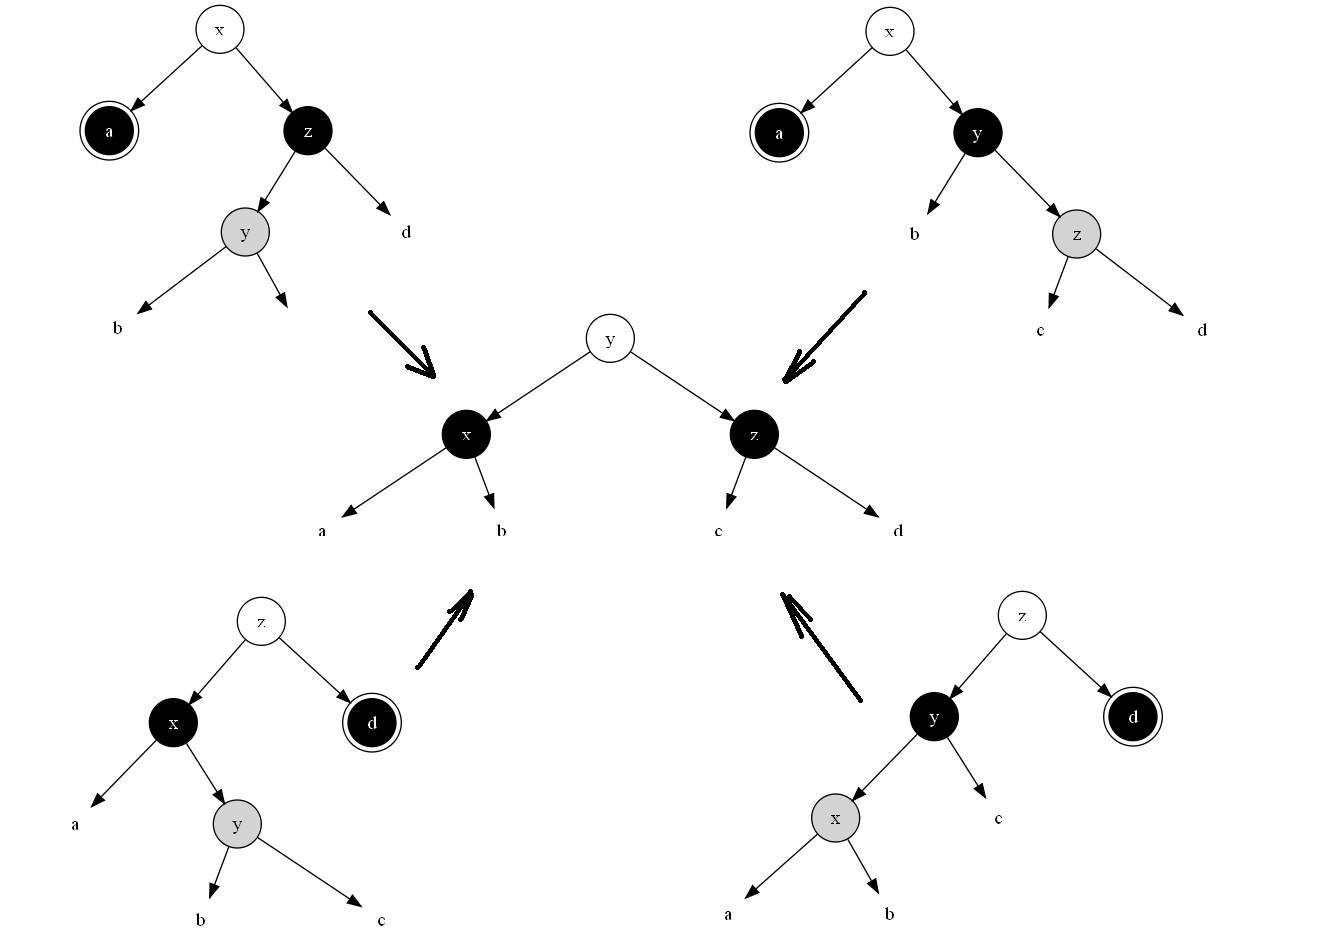
\includegraphics[scale=0.4]{img/del-case1.eps}
   \caption{Fix the doubly black by rotation, the sibling of the doubly-black node is black, and it has one red child.} \label{fig:del-case1}
\end{figure}

The handling of these 4 sub-cases can be defined on top of formula \ref{eq:db-nil}. 

\be
fixBlack^2(T) = \left \{
  \begin{array}
  {r@{\quad:\quad}l}
  ... & ... \\
  node(\mathcal{C}, node(\mathcal{B}, mkBlk(A), x, B), y, node(\mathcal{B}, C, z, D)) & p 1.1 \\
  node(\mathcal{C}, node(\mathcal{B}, A, x, B), y, node(\mathcal{B}, C, z, mkBlk(D))) & p 1.2 \\
  ... & ...
  \end{array}
\right .
\label{eq:db-case-1}
\ee

where $p 1.1$ and $p 1.2$ each represent 2 patterns as the following.

\[
p 1.1 = \left \{ \begin{array}{l}
  node(\mathcal{C}, A, x, node(\mathcal{B}, node(\mathcal{R}, B, y, C), z, D)) \land Color(A) = \mathcal{B}^2 \\
  \lor \\
  node(\mathcal{C}, A, x, node(\mathcal{B}, B, y, node(\mathcal{R}, C, z, D))) \land Color(A) = \mathcal{B}^2
  \end{array} \right \}
\]

\[
p 1.2 = \left \{ \begin{array}{l}
  node(\mathcal{C}, node(\mathcal{B}, A, x, node(\mathcal{R}, B, y, C)), z, D) \land Color(D) = \mathcal{B}^2 \\
  \lor \\
  node(\mathcal{C}, node(\mathcal{B}, node(\mathcal{R}, A, x, B), y, C), z, D) \land Color(D) = \mathcal{B}^2
  \end{array} \right \}
\]

Besides the above cases, there is another one that not only the sibling
of the doubly-black node is black, but also its two children are black. 
We can change the color of the sibling node to red; resume the 
doubly-black node to black and propagate the doubly-blackness one level 
up to the parent node as shown in figure \ref{fig:del-case2}. Note that
there are two symmetric sub-cases. This case is described in \cite{CLRS} 
as case 2.

\begin{figure}[htbp]
  \centering
  \setlength{\unitlength}{1cm}
  \begin{picture}(10, 4)
  \put(5, 2){$\Longrightarrow$}
  \subfloat[Color of $x$ can be either black or red.]{\includegraphics[scale=0.4]{img/case2-a.ps}}
  \subfloat[If $x$ was red, then it becomes black, otherwise, it becomes doubly-black.]{\includegraphics[scale=0.4]{img/case2-a1.ps}}
  \end{picture}
  \\
  \begin{picture}(10, 5)
  \put(5, 2){$\Longrightarrow$}
  \subfloat[Color of $y$ can be either black or red.]{\includegraphics[scale=0.4]{img/case2-b.ps}}
  \subfloat[If $y$ was red, then it becomes black, otherwise, it becomes doubly-black.]{\includegraphics[scale=0.4]{img/case2-b1.ps}}
  \end{picture}
  \\
  \begin{picture}(1, 0.5)\end{picture} %pad
  \caption{propagate the blackness up.} \label{fig:del-case2}
\end{figure}

We go on adding this fixing after formula \ref{eq:db-case-1}.

\be
fixBlack^2(T) = \left \{
  \begin{array}
  {r@{\quad:\quad}l}
  ... & ... \\
  mkBlk(node(\mathcal{C}, mkBlk(A), x, node(\mathcal{R}, B, y, C))) & p 2.1 \\
  mkBlk(node(\mathcal{C}, node(\mathcal{R}, A, x, B), y, mkBlk(C))) & p 2.2 \\
  ... & ...
  \end{array}
\right .
\label{eq:db-case-2}
\ee

where $p 2.1$ and $p 2.2$ are two patterns as below.

\[
p 2.1 = \left \{ \begin{array}{l}
  node(\mathcal{C}, A, x, node(\mathcal{B}, B, y, C)) \land \\
  Color(A) = \mathcal{B}^2 \land Color(B) = Color(C) = \mathcal{B}
  \end{array} \right \}
\]

\[
p 2.2 = \left \{ \begin{array}{l}
  node(\mathcal{C}, node(\mathcal{B}, A, x, B), y, C) \land \\
  Color(C) = \mathcal{B}^2 \land Color(A) = Color(B) = \mathcal{B}
  \end{array} \right \}
\]

There is a final case left, that the sibling of the doubly-black node is red.
We can do a rotation to change this case to pattern $p 1.1$ or $p 1.2$.
Figure \ref{fig:del-case3} shows about it.

\begin{figure}[htbp]
  \centering
  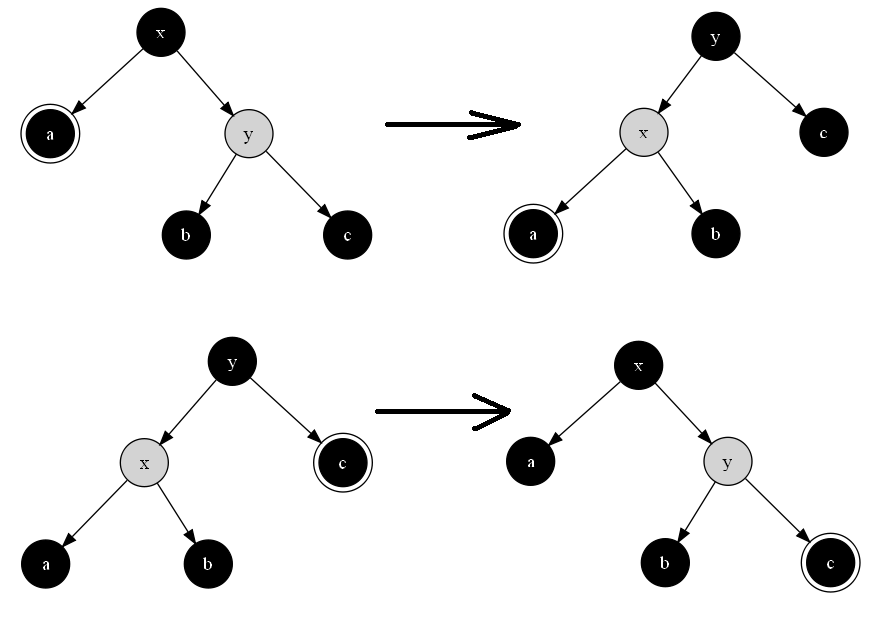
\includegraphics[scale=0.4]{img/del-case3.eps}
  \caption{The sibling of the doubly-black node is red.} \label{fig:del-case3}
\end{figure}

We can finish formula \ref{eq:db-case-2} with \ref{eq:db-case-3}.

\be
fixBlack^2(T) = \left \{
  \begin{array}
  {r@{\quad:\quad}l}
  ... & ... \\
  fixBlack^2(\mathcal{B}, fixBlack^2(node(\mathcal{R}, A, x, B), y, C) & p 3.1 \\
  fixBlack^2(\mathcal{B}, A, x, fixBlack^2(node(\mathcal{R}, B, y, C)) & p 3.2 \\
  T & otherwise
  \end{array}
\right .
\label{eq:db-case-3}
\ee

where $p 3.1$ and $p 3.2$ are two patterns as the following.

\[
p 3.1 = \{ Color(T) = \mathcal{B} \land Color(L) = \mathcal{B}^2 \land Color(R) = \mathcal{R} \}
\]

\[
p 3.2 = \{ Color(T) = \mathcal{B} \land Color(L) = \mathcal{R} \land Color(R) = \mathcal{B}^2 \}
\]


This two cases are described in \cite{CLRS} as case 1.

Fixing the doubly-black node with all above different cases is a recursive function. 
There are two termination conditions. One contains pattern $p 1.1$ and $p 1.2$, 
The doubly-black node was eliminated. The other cases may continuously propagate the 
doubly-blackness from bottom to top till the root.
Finally the algorithm marks the root node as black anyway. The doubly-blackness will be
removed.

Put formula \ref{eq:db-nil}, \ref{eq:db-case-1}, \ref{eq:db-case-2}, and \ref{eq:db-case-3}
together, we can write the final Haskell program.

\begin{lstlisting}
fixDB::Color -> RBTree a -> a -> RBTree a -> RBTree a
fixDB color BBEmpty k Empty = Node BB Empty k Empty
fixDB color BBEmpty k r = Node color Empty k r
fixDB color Empty k BBEmpty = Node BB Empty k Empty
fixDB color l k BBEmpty = Node color l k Empty
-- the sibling is black, and it has one red child
fixDB color a@(Node BB _ _ _) x (Node B (Node R b y c) z d) = 
      Node color (Node B (makeBlack a) x b) y (Node B c z d)
fixDB color a@(Node BB _ _ _) x (Node B b y (Node R c z d)) = 
      Node color (Node B (makeBlack a) x b) y (Node B c z d)
fixDB color (Node B a x (Node R b y c)) z d@(Node BB _ _ _) = 
      Node color (Node B a x b) y (Node B c z (makeBlack d))
fixDB color (Node B (Node R a x b) y c) z d@(Node BB _ _ _) = 
      Node color (Node B a x b) y (Node B c z (makeBlack d))
-- the sibling and its 2 children are all black, propagate the blackness up
fixDB color a@(Node BB _ _ _) x (Node B b@(Node B _ _ _) y c@(Node B _ _ _))
    = makeBlack (Node color (makeBlack a) x (Node R b y c))
fixDB color (Node B a@(Node B _ _ _) x b@(Node B _ _ _)) y c@(Node BB _ _ _)
    = makeBlack (Node color (Node R a x b) y (makeBlack c))
-- the sibling is red
fixDB B a@(Node BB _ _ _) x (Node R b y c) = fixDB B (fixDB R a x b) y c
fixDB B (Node R a x b) y c@(Node BB _ _ _) = fixDB B a x (fixDB R b y c)
-- otherwise
fixDB color l k r = Node color l k r
\end{lstlisting}

Compare to the insertion algorithm, we can find the difference in
terms of complexity.

\subsection*{Exercise}
\begin{itemize}
\item As we mentioned in this section, deletion can be implemented
by just marking the node as deleted without actually removing it.
Once the number of marked nodes exceeds 50\% of the total node
number, a tree re-build is performed. Try to implement this
method in your favorate programming language.
\end{itemize}

Basically, we finish this chapter. 
TODO: list the imperative insertion/deletion algorithm for comparison purpose.

\subsubsection*{Python red black tree insertion, imperative}

The python version imperative implementation uses the method described in CLRS.

\lstset{language=Python}
\begin{lstlisting}
def rb_insert(t, key): #returns the new root
    root = t
    x = Node(key)
    parent = None
    while(t):
        parent = t
        if(key < t.key):
            t = t.left
        else:
            t = t.right
    if parent is None: #tree is empty
        root = x
    elif key < parent.key:
        parent.set_left(x)
    else:
        parent.set_right(x)
    return rb_insert_fix(root, x)
\end{lstlisting}

Compare the above source code and the one in binary search tree\cite{bst-lxy}. The only difference are we simplified the program by using set\_left()/set\_right() member functions, and there is a rb\_insert\_fix() function call to fix the red node violation.

There are 3 cases described in CLRS, and if we take the left-right symmetric into consideration. there are total 6 cases. Among them two cases can be merged together, because they are all have uncle node in red color, we can toggle the parent color and uncle color to black and set grand parent color to red. After this merge the 5 cases fixing version can be implemented as the following.

\begin{lstlisting}
# Fix the red->red violation
def rb_insert_fix(t, x):
    while(x.parent and x.parent.color==RED):
        if x.uncle().color == RED:
            #case 1: ((a:R x:R b) y:B c:R) ==> ((a:R x:B b) y:R c:B)
            set_color([x.parent, x.grandparent(), x.uncle()],
                      [BLACK, RED, BLACK])
            x = x.grandparent()
        else:
            if x.parent == x.grandparent().left:
                if x == x.parent.right:
                    #case 2: ((a x:R b:R) y:B c) ==> case 3
                    x = x.parent
                    t=left_rotate(t, x)
                # case 3: ((a:R x:R b) y:B c) ==> (a:R x:B (b y:R c))
                set_color([x.parent, x.grandparent()], [BLACK, RED])
                t=right_rotate(t, x.grandparent())
            else:
                if x == x.parent.left:
                    #case 2': (a x:B (b:R y:R c)) ==> case 3'
                    x = x.parent
                    t = right_rotate(t, x)
                # case 3': (a x:B (b y:R c:R)) ==> ((a x:R b) y:B c:R)
                set_color([x.parent, x.grandparent()], [BLACK, RED])
                t=left_rotate(t, x.grandparent())
    t.color = BLACK
    return t
\end{lstlisting}

TODO: discuss about the performance overhead

If we compare the results from the functional implementation and from the imperative one, we can 
find there is difference. Even if we insert the same element into the same red black tree, the
results varies. This is because the functional way focus on expressive of the program, and there 
is a bit performance overhead in it. Okasaki discussed about the difference in his paper\cite{okasaki}.
And he show the result that the computation time is still $O(log n)$. It is possible to use a 
similar way to the imperative implementation. And that's a kind of fine tune in the 'balance()'
function. But it will loss the expressive merit.


\begin{thebibliography}{99}

\bibitem{CLRS}
Thomas H. Cormen, Charles E. Leiserson, Ronald L. Rivest and Clifford Stein. 
``Introduction to Algorithms, Second Edition''. ISBN:0262032937. The MIT Press. 2001

\bibitem{okasaki}
Chris Okasaki. ``FUNCTIONAL PEARLS Red-Black Trees in a Functional Setting''. J. Functional Programming. 1998

\bibitem{okasaki-blog}
Chris Okasaki. ``Ten Years of Purely Functional Data Structures''. http://okasaki.blogspot.com/2008/02/ten-years-of-purely-functional-data.html

\bibitem{wiki}
Wikipedia. ``Red-black tree''. http://en.wikipedia.org/wiki/Red-black\_tree

\bibitem{lyn}
Lyn Turbak. ``Red-Black Trees''. cs.wellesley.edu/~cs231/fall01/red-black.pdf Nov. 2, 2001.

\bibitem{sgi-stl}
http://www.sgi.com/tech/stl/

\bibitem{hj-stl}
Hou Jie. ``The annotated STL sources (using SGI STL)''. ISBN:7-5609-2699-1 http://press.hust.edu.cn. 2002.

\end{thebibliography}

\ifx\wholebook\relax\else
\end{document}
\fi


\ifx\wholebook\relax \else
% ------------------------ 

\documentclass{article}
%------------------- Other types of document example ------------------------
%
%\documentclass[twocolumn]{IEEEtran-new}
%\documentclass[12pt,twoside,draft]{IEEEtran}
%\documentstyle[9pt,twocolumn,technote,twoside]{IEEEtran}
%
%-----------------------------------------------------------------------------
%%
% loading packages
%
\newif\ifpdf
\ifx\pdfoutput\undefined % We're not running pdftex
  \pdffalse
\else
  \pdftrue
\fi
%
%
\ifpdf
  \RequirePackage[pdftex,%
            CJKbookmarks,%
       bookmarksnumbered,%
              colorlinks,%
          linkcolor=blue,%
              hyperindex,%
        plainpages=false,%
       pdfstartview=FitH]{hyperref}
\else
  \RequirePackage[dvipdfm,%
             CJKbookmarks,%
        bookmarksnumbered,%
               colorlinks,%
           linkcolor=blue,%
               hyperindex,%
         plainpages=false,%
        pdfstartview=FitH]{hyperref}
  \AtBeginDvi{\special{pdf:tounicode GBK-EUC-UCS2}} % GBK -> Unicode
\fi
\usepackage{hyperref}

% other packages
%-----------------------------------------------------------------------------
\usepackage{graphicx, color}
\usepackage{CJK}
%
% for programming 
%
\usepackage{verbatim}
\usepackage{listings}


\lstdefinelanguage{Smalltalk}{
  morekeywords={self,super,true,false,nil,thisContext}, % This is overkill
  morestring=[d]',
  morecomment=[s]{"}{"},
  alsoletter={\#:},
  escapechar={!},
  literate=
    {BANG}{!}1
    {UNDERSCORE}{\_}1
    {\\st}{Smalltalk}9 % convenience -- in case \st occurs in code
    % {'}{{\textquotesingle}}1 % replaced by upquote=true in \lstset
    {_}{{$\leftarrow$}}1
    {>>>}{{\sep}}1
    {^}{{$\uparrow$}}1
    {~}{{$\sim$}}1
    {-}{{\sf -\hspace{-0.13em}-}}1  % the goal is to make - the same width as +
    %{+}{\raisebox{0.08ex}{+}}1		% and to raise + off the baseline to match -
    {-->}{{\quad$\longrightarrow$\quad}}3
	, % Don't forget the comma at the end!
  tabsize=2
}[keywords,comments,strings]

\lstloadlanguages{C++, Lisp, Haskell, Python, Smalltalk}

% ======================================================================

\def\BibTeX{{\rm B\kern-.05em{\sc i\kern-.025em b}\kern-.08em
    T\kern-.1667em\lower.7ex\hbox{E}\kern-.125emX}}

\newtheorem{theorem}{Theorem}

%
% mathematics
%
\newcommand{\be}{\begin{equation}}
\newcommand{\ee}{\end{equation}}
\newcommand{\bmat}[1]{\left( \begin{array}{#1} }
\newcommand{\emat}{\end{array} \right) }
\newcommand{\VEC}[1]{\mbox{\boldmath $#1$}}

% numbered equation array
\newcommand{\bea}{\begin{eqnarray}}
\newcommand{\eea}{\end{eqnarray}}

% equation array not numbered
\newcommand{\bean}{\begin{eqnarray*}}
\newcommand{\eean}{\end{eqnarray*}}

\RequirePackage{CJK,CJKnumb,CJKulem,CJKpunct}
% we use CJK as default environment
\AtBeginDocument{\begin{CJK*}{GBK}{song}\CJKtilde\CJKindent\CJKcaption{GB}}
\AtEndDocument{\clearpage\end{CJK*}}

%
% loading packages
%

\RequirePackage{ifpdf}

%
%
\ifpdf
  \RequirePackage[pdftex,%
       bookmarksnumbered,%
              colorlinks,%
          linkcolor=blue,%
              hyperindex,%
        plainpages=false,%
       pdfstartview=FitH]{hyperref}
\else
  \RequirePackage[dvipdfm,%
        bookmarksnumbered,%
               colorlinks,%
           linkcolor=blue,%
               hyperindex,%
         plainpages=false,%
        pdfstartview=FitH]{hyperref}
\fi
\usepackage{hyperref}

% other packages
%--------------------------------------------------------------------------
\usepackage{graphicx, color}
\usepackage{subfig}

\usepackage{amsmath, amsthm, amssymb} % for math
\usepackage{exercise} % for exercise

%
% for programming 
%
\usepackage{verbatim}
\usepackage{listings}
%\usepackage{algorithmic} %old version; we can use algorithmicx instead
\usepackage{algorithm} 
\usepackage[noend]{algpseudocode} %for pseudo code, include algorithmicsx automatically
\usepackage{makeidx} % for index support


\lstdefinelanguage{Smalltalk}{
  morekeywords={self,super,true,false,nil,thisContext}, % This is overkill
  morestring=[d]',
  morecomment=[s]{"}{"},
  alsoletter={\#:},
  escapechar={!},
  literate=
    {BANG}{!}1
    {UNDERSCORE}{\_}1
    {\\st}{Smalltalk}9 % convenience -- in case \st occurs in code
    % {'}{{\textquotesingle}}1 % replaced by upquote=true in \lstset
    {_}{{$\leftarrow$}}1
    {>>>}{{\sep}}1
    {^}{{$\uparrow$}}1
    {~}{{$\sim$}}1
    {-}{{\sf -\hspace{-0.13em}-}}1  % the goal is to make - the same width as +
    %{+}{\raisebox{0.08ex}{+}}1		% and to raise + off the baseline to match -
    {-->}{{\quad$\longrightarrow$\quad}}3
	, % Don't forget the comma at the end!
  tabsize=2
}[keywords,comments,strings]

\lstloadlanguages{C++, Lisp, Haskell, Python, Smalltalk}

% ======================================================================

\def\BibTeX{{\rm B\kern-.05em{\sc i\kern-.025em b}\kern-.08em
    T\kern-.1667em\lower.7ex\hbox{E}\kern-.125emX}}

%
% mathematics
%
\newcommand{\be}{\begin{equation}}
\newcommand{\ee}{\end{equation}}
\newcommand{\bmat}[1]{\left( \begin{array}{#1} }
\newcommand{\emat}{\end{array} \right) }
\newcommand{\VEC}[1]{\mbox{\boldmath $#1$}}

% numbered equation array
\newcommand{\bea}{\begin{eqnarray}}
\newcommand{\eea}{\end{eqnarray}}

% equation array not numbered
\newcommand{\bean}{\begin{eqnarray*}}
\newcommand{\eean}{\end{eqnarray*}}

\newtheorem{theorem}{Theorem}[section]
\newtheorem{lemma}[theorem]{Lemma}
\newtheorem{proposition}[theorem]{Proposition}
\newtheorem{corollary}[theorem]{Corollary}


\setcounter{page}{1}

\begin{document}

\fi
%--------------------------

% ================================================================
%                 COVER PAGE
% ================================================================

\title{AVL tree}

\author{Liu~Xinyu
\thanks{{\bfseries Liu Xinyu } \newline
  Email: liuxinyu95@gmail.com \newline}
  }

\markboth{AVL tree}{AlgoXY}

\maketitle

\ifx\wholebook\relax
\chapter{AVL tree}
\fi

% ================================================================
%                 Introduction
% ================================================================
\section{Introduction}
\label{introduction} \index{AVL tree}

\subsection{How to measure the balance of a tree?}
Besides red-black tree, are there any other intuitive solutions of self-balancing
binary search tree? In order to measure how balancing a binary search tree,
one idea is to compare the height of the left sub-tree and right sub-tree.
If they differs a lot, the tree isn't well balanced. Let's denote the 
difference height between two children as below

\be
  \delta(T) = |L| - |R|
\ee

Where $|T|$ means the height of tree $T$, and $L$, $R$ denotes the left
sub-tree and right sub-tree.

If $\delta(T) = 0$, The tree is defnitely balanced. For example, a 
complete binary tree has $N=2^h-1$ nodes for height $h$. There is
no empty branches unless the leafs. Another trivial case is empty 
tree. $\delta(\phi) = 0$. The less absolute value of $\delta(T)$
the more balancing the tree is. 

We define $\delta(T)$ as the {\em balance factor} of a binary search
tree.

% ================================================================
% Definition
% ================================================================
\section{Definition of AVL tree}
\index{AVL tree!definition}

An AVL tree is a special binary search tree, that all sub-trees 
satisfying the following criteria.

\be
  |\delta(T)| \leq 1
\ee

The absolute value of balance factor is less than or equal to 1, which
means there are only three valid values, -1, 0 and 1.

Why AVL tree can keep the tree balanced? In other words, Can this definition
ensure the height of the tree as $O(\lg N)$ where $N$ is the number of
the nodes in the tree? Let's prove this fact.

For an AVL tree of height $h$, The number of nodes varies. It can have at
most $2^h-1$ nodes for a complete binary tree. We are interesting about
how many nodes there are at least. Let's denote the minimum number of nodes
for height $h$ AVL tree as $N(h)$. It's obvious for the trivial cases 
as below.

\begin{itemize}
\item For empty tree, $h=0$, $N(0)=0$;
\item For a singlton root, $h=1$, $N(1)=1$;
\end{itemize}

What's the situation for common case $N(h)$? Figure \ref{fig:N-h-relation}
shows an AVL tree $T$ of height $h$. It contains three part, the root node,
and two sub trees $A, B$. We have the following fact.

\be
  h= max(height(L), height(R)) + 1
\ee

We immediately know that, there must be one child has height $h-1$. Let's 
say $height(A) = h-1$. According to the definition of AVL tree, we have.
$|height(A)-height(B)| \leq 1$. This leads to the fact that the height of
other tree $B$ can't be lower than $h-2$, So the total number of the nodes
of $T$ is the number of nodes in tree $A$, and $B$ plus 1 (for the root node).
We exclaim that.

\be
  N(h) = N(h-1) + N(h-2) + 1
  \label{eq:Fibonacci-like}
\ee

\begin{figure}[htbp]
   \centering
   \includegraphics[scale=0.5]{img/Nh-lvr.ps}
   \caption{An AVL tree with height $h$, one of the sub-tree with height $h-1$, the other is $h-2$} \label{fig:N-h-relation}
\end{figure}

This recusion reminds us the famous Fibonacci series. Actually we can 
transform it to Fibonacci series by defining $N'(h) = N(h)+1$. So equation
\ref{eq:Fibonacci-like} changes to.

\be
  N'(h) = N'(h-1) + N'(h-2)
\ee

\begin{lemma}
\label{lemma:N-phi}
Let $N(h)$ be the minimum number of nodes for an AVL tree with
height $h$. and $N'(h) = N(h) + 1$, then
\be
  N'(h) \geq \phi^h
\ee

Where $\phi = \frac{\sqrt{5}+1}{2}$ is the golden ratio.
\end{lemma}

\begin{proof}
For the trivial case, we have
\begin{itemize}
\item $h=0$, $N'(0) = 1 \geq \phi^0 = 1$
\item $h=1$, $N'(1) = 2 \geq \phi^1 = 1.618...$
\end{itemize}

For the induction case, suppose $N'(h) \geq \phi^h$.
\[
  \begin{array}{lll}
  N'(h+1) & = N'(h) + N'(h-1) & \{Fibonacci\} \\
          & \geq \phi^h + \phi^{h-1} & \\
          & = \phi^{h-1}(\phi + 1) & \{\phi + 1 = \phi^2 = \frac{\sqrt{5}+3}{2}\} \\
          & = \phi^{h+1}
 \end{array}
\]
\end{proof}

From Lemma \ref{lemma:N-phi}, we immedately get

\be
  h \leq log_{\phi}(N+1) = log_{\phi}(2) \cdot \lg (N+1) \approx 1.44 \lg (N+1)
  \label{eq:AVL-height}
\ee

It tells that the height of AVL tree is proportion to $O(\lg N)$, which
means that AVL tree is balanced.

During the basic mutable tree operations such as insertion and deletion,
if the balance factor changes to any invalide value, some fixing has
to be performed to resume $|\delta|$ within 1. Most implementations utilize
tree rotations. In this chapter, we'll show the pattern matching solution
which is inspired by Okasaki's red-black tree solution\cite{okasaki}.
Because of this modify-fixing approach, AVL tree is also a kind of 
self-balancing binary search tree. For comparison purpose, we'll also
show the procedural algorithms.

Of course we can compute the $\delta$ value recursively, another option
is to store the balance factor inside each nodes, and update them
when we modify the tree. The latter one avoid computing the same value
every time.

Based on this idea, we can add one data field $\delta$ to the original
binary search tree as the following C++ code exmample.

\lstset{language=C++}
\begin{lstlisting}
template <class T>
struct node{
  int delta;
  T key;
  node* left;
  node* right;
  node* parent;
};
\end{lstlisting}

In purely functional setting, some implementation use different 
constructor to store the $\delta$ information. for example in 
\cite{hackage}, there are 4 constructors, E, N, P, Z defined.
E for empty tree, N for tree with negative 1 balance factor,
P for tree with positive 1 balance factor and Z for zero case.

In this chapter, we'll explicitly store the balance factor inside
the node.

\lstset{language=Haskell}
\begin{lstlisting}
data AVLTree a = Empty
               | Br (AVLTree a) a (AVLTree a) Int 
\end{lstlisting}

The immutable operations, including looking up, finding the maximum
and minimum elements are all same as the binary search tree. We'll
skip them and focus on the mutable operations.

% ================================================================
%                 Insertion
% ================================================================
\section{Insertion}
\index{AVL tree!insertion}

Insert a new element to an AVL tree may vialate the AVL tree property
that the $\delta$ absolute value exceeds 1. To resume it, one option
is to do the tree rotation according to the different insertion cases.
Most implementation is based on this approach

Another way is to use the similar pattern matching method mentioned by
Okasaki in his red-black tree implementation \cite{okasaki}. Inspried 
by this idea, it is possible to provide a simiple and intuitive
solution.  

When insert a new key to the AVL tree, the balance factor of the 
root may changes in range $[-1, 1]$, and the height may increase
at most by one, which we need recursively use this information
to update the $\delta$ value in upper level nodes. We can define
the result of the insertion algorithm as a pair of data 
$(T', \Delta H)$. Where $T'$ is the new tree and $\Delta H$ is the
increament of height. Let's denote function $first(pair)$ which 
can return the first element in a pair. We can modify
the binary search tree insertion algorithm as the following to
handle AVL tree.

\be
insert(T, k) = first(ins(T, k))
\ee

where 

\be
ins(T, k) = \left \{
  \begin{array}
  {r@{\quad:\quad}l}
  (node(\phi, k, \phi, 0), 1) & T = \phi \\
  (tree(ins(L, k), Key, (R, 0)), \Delta) & k < Key \\
  (tree((L, 0), Key, ins(R, k)), \Delta) & otherwise
  \end{array}
\right.
\label{eq:ins}
\ee 

$L, R, Key, \Delta$ represent the left child, right child, the key and
the balance factor of a tree.

\[
  \begin{array}{l}
  L = left(T) \\
  R = right(T) \\
  Key = key(T) \\
  \Delta = \delta(T)
  \end{array}
\]

When we insert a new key $k$ to a AVL tree $T$, if the tree is 
empty, we just need create a leaf node with $k$, set the balance
factor as 0, and the height is increased by one. This is the trivial
case. Function $node()$ is defined to build a tree by taking a
left sub-tree, a right sub-tree, a key and a balance factor.

If $T$ isn't empty, we need compare the $Key$ with $k$.
If $k$ is less than the key, we recursively insert it to the left
child, otherwise we insert it into the right child.

As we defined above, the result of the recursive insertion is a 
pair like $(L', \Delta H_l)$, we need do balancing adjustment as well
as updating the increment of height. Function $tree()$ is defined
to dealing with this task. It takes 4 arguments as $(L', \Delta H_l)$,
$Key$, $(R', \Delta H_r)$, and $\Delta$. The result of this function
is defined as $(T', \Delta H)$, where $T'$ is the new tree after 
adjustment, and $\Delta H$ is the new increament of height which is 
defined as

\be
  \Delta H = |T'| - |T|
\ee

This can be further detailed deduced in 4 cases.

\be
\begin{array}{rl}
  \Delta H & = |T'| - |T| \\
              & = 1 + max(|R'|, |L'|) - (1 + max(|R|, |L|)) \\
              & = max(|R'|, |L'|) - max(|R|, |L|) \\
              & = \left \{
                  \begin{array}{r@{\quad:\quad}l}
                  \Delta H_r & \Delta \geq 0 \land \Delta' \geq 0 \\
                  \Delta + \Delta H_r & \Delta \leq 0 \land \Delta' \geq 0 \\
                  \Delta H_l - \Delta & \Delta \geq 0 \land \Delta' \leq 0 \\
                  \Delta H_l & otherwise
                  \end{array} \right .
\end{array}
\ee

To prove this equation, note the fact that the height can't increase
both in left and right with only one insertion.

These 4 cases can be explained from the definition of balance factor
definition that it equal to the difference from the right sub tree
and left sub tree.

\begin{itemize}
\item If $\Delta \geq 0$ and $\Delta' \geq 0$, it means that the height
of right sub tree isn't less than the height of left sub tree both
before insertion and after insertion. In this case, the increment in
height of the tree is only `contributed' from the right sub tree, which
is $\Delta H_r$.

\item If $\Delta \leq 0$, which means the height of left sub tree isn't
less than the height of right sub tree before, and it becomes 
$\Delta' \geq 0$,
which means that the height of right sub tree increases due to insertion, 
and the left side keeps same ($|L'|=|L|$). So the increment in height is
\[
\begin{array}{rll}
\Delta H & = max(|R'|, |L'|) - max (|R|, |L|) & \{\Delta \leq 0 \land \Delta' \geq 0 \}\\
         & = |R'|-|L'| & \{|L|=|L'| \}\\
         & = |R|+\Delta H_r - |L| & \\
         & = \Delta + \Delta H_r &
\end{array}
\]

\item For the case $\Delta \geq 0 \land \Delta' \leq 0$, Similar as the
second one, we can get.

\[
\begin{array}{rll}
\Delta H & = max(|R'|, |L'|) - max (|R|, |L|) & \{\Delta \geq 0 \land \Delta' \leq 0 \}\\
         & = |L'|-|R| & \\
         & = |L|+\Delta H_l - |R| & \\
         & = \Delta H_l - \Delta&
\end{array}
\]

\item For the last case, the both $\Delta$ and $\Delta'$ is no bigger than
zero, which means the height left sub tree is always greater than or equal
 to the right sub tree, so the increament in height is only `contributed'
from the right sub tree, which is $\Delta H_l$.
\end{itemize}

The next problem in front of us is how to determin the new balancing
factor value $\Delta'$ before performing balancing adjustment.
According to the definition of AVL tree, the balancing factor is the
height of right sub tree minus the hight of right sub tree. We have
the following facts.

\be
\begin{array}{rl}
\Delta' & = |R'| - |L'| \\
        & = |R| + \Delta H_r - (|L| + \Delta H_l) \\
        & = |R| - |L| + \Delta H_r - \Delta H_l \\
        & = \Delta + \Delta H_r - \Delta H_l
\end{array}
\ee

With all these changes in height and balancing factor get clear, it's
possible to define the $tree()$ function mentioned in (\ref{eq:ins}).

\be
tree((L', \Delta H_l), Key, (R', \Delta H_r), \Delta) = 
  balance (node(L', Key, R', \Delta'), \Delta H)
\ee

Before we moving into details of balancing adjustment, let's translate
the aboving equations to real programs in Haskell.

First is the insert function.

\lstset{language=Haskell}
\begin{lstlisting}
insert::(Ord a)=>AVLTree a -> a -> AVLTree a
insert t x = fst $ ins t where
    ins Empty = (Br Empty x Empty 0, 1)
    ins (Br l k r d) 
        | x < k     = tree (ins l) k (r, 0) d
        | x == k    = (Br l k r d, 0)
        | otherwise = tree (l, 0) k (ins r) d
\end{lstlisting} %$

Here we also handle the case that inserting a duplicated key (which
means the key has already existed.) as just overwriting.

\begin{lstlisting}
tree::(AVLTree a, Int) -> a -> (AVLTree a, Int) -> Int -> (AVLTree a, Int)
tree (l, dl) k (r, dr) d = balance (Br l k r d', delta) where
    d' = d + dr - dl
    delta = deltaH d d' dl dr
\end{lstlisting}

And the definition of height increment is as below.

\begin{lstlisting}
deltaH :: Int -> Int -> Int -> Int -> Int
deltaH d d' dl dr 
       | d >=0 && d' >=0 = dr
       | d <=0 && d' >=0 = d+dr
       | d >=0 && d' <=0 = dl - d
       | otherwise = dl
\end{lstlisting}

\subsection{Balancing adjustment}
\index{AVL tree!balancing}
As the pattern matching approach is adopted in doing rebalancing.
We need consider what kind of patterns violate the AVL tree property.

Figure \ref{fig:insert-fix} shows the 4 cases which need fix. For all
these 4 cases the balacing factors are either -2, or +2 which exceed
the range of $[-1, 1]$. After balancing adjustment, this factor turns
to be 0, which means the height of left sub tree is equal to the right
sub tree.

\begin{figure}[htbp]
   \begin{center}
     \setlength{\unitlength}{1cm}
     \begin{picture}(15, 15)
        % arrows
        \put(4.5, 9.5){\vector(1, -1){1}}
        \put(4.5, 5){\vector(1, 1){1}}
        \put(10, 9.5){\vector(-1, -1){1}}
        \put(10, 5){\vector(-1, 1){1}}
        % delta values
        \put(5, 13){$\delta(z) = -2$}
        \put(2.5, 12){$\delta(y) = -1$}
        \put(10, 13){$\delta(x) = 2$}
        \put(11.5, 11.5){$\delta(y) = 1$}
        \put(1.5, 5.5){$\delta(z) = -2$}
        \put(3.5, 4){$\delta(x) = 1$}
        \put(12, 5.5){$\delta(x) = 2$}
        \put(10.5, 4){$\delta(z) = -1$}
        \put(7.5, 10){$\delta'(y) = 0$}
        % graphics
	\put(0, 7){\includegraphics[scale=0.5]{img/insert-ll.ps}}
        \put(0, 0){\includegraphics[scale=0.5]{img/insert-lr.ps}}
        \put(7, 7){\includegraphics[scale=0.5]{img/insert-rr.ps}}
        \put(8.5, 0){\includegraphics[scale=0.5]{img/insert-rl.ps}}
        \put(2, 5){\includegraphics[scale=0.5]{img/insert-fixed.ps}}
      \end{picture}
     \caption{4 cases for balancing a AVL tree after insertion} \label{fig:insert-fix}
  \end{center}
\end{figure}

We call these four cases left-left lean, right-right lean, right-left lean,
and left-right lean cases in clock-wise direction from top-left. We denote
the balancing factor before fixing as $\delta(x), \delta(y)$, and $\delta(z)$, while after fixing, they changes to $\delta'(x), \delta'(y)$, and
$\delta'(z)$ respectively. 

We'll next prove that, after fixing, we have $\delta(y)=0$ for all
four cases, and we'll provide the result values of $\delta'(x)$ and 
$\delta'(z)$.

\subsubsection*{Left-left lean case}

As the structure of sub tree $x$ doesn't change due to fixing, we immediately get
$\delta'(x) = \delta(x)$. 

Since $\delta(y) = -1$ and $\delta(z) = -2$, we have

\be
  \begin{array}{l}
  \delta(y) = |C| - |x| = -1 \Rightarrow |C| = |x| - 1 \\
  \delta(z) = |D| - |y| = -2 \Rightarrow |D| = |y| - 2
  \end{array}
  \label{eq:ll-cd}
\ee

After fixing.

\be
  \begin{array}{rll}
  \delta'(z) & = |D| - |C| & \{ From (\ref{eq:ll-cd}) \}\\
             & = |y| - 2 - (|x| - 1) & \\
             & = |y| - |x| - 1 & \{  x \text{ is child of } y \Rightarrow |y|-|x| = 1\} \\
             & = 0 &
  \end{array}
  \label{eq:ll-delta-z}
\ee

For $\delta'(y)$, we have the following fact after fixing.

\be
  \begin{array}{rll}
  \delta'(y) & = |z| - |x| & \\
             & = 1 + max(|C|, |D|) - |x| & \{ \text{By (\ref{eq:ll-delta-z}), we have} |C| = |D|\} \\
             & = 1 + |C| - |x| & \{ \text{By (\ref{eq:ll-cd})}\} \\
             & = 1 + |x| - 1 - |x| & \\
             & = 0 &
  \end{array}
\ee

Summarize the above results, the left-left lean case adjust the balancing
factors as the following.

\be
  \begin{array}{l}
  \delta'(x) = \delta(x) \\
  \delta'(y) = 0 \\
  \delta'(z) = 0
  \end{array}
\ee

\subsubsection*{Right-right lean case}

Since right-right case is symmetric to left-left case, we can easily achieve the result balancing factors as

\be
  \begin{array}{l}
  \delta'(x) = 0 \\
  \delta'(y) = 0 \\
  \delta'(z) = \delta(z)
  \end{array}
  \label{eq:rr-result}
\ee

\subsubsection*{Right-left lean case}

First let's consider $\delta'(x)$. After balance fixing, we have.

\be
  \delta'(x) = |B| - |A|
  \label{eq:rl-dx}
\ee

Before fixing, if we calculate the height of $z$, we can get.

\be
  \begin{array}{rll}
  |z| & = 1 + max(|y|, |D|) &  \{ \delta(z) = -1 \Rightarrow |y| > |D|\} \\
      & = 1 + |y| & \\
      & = 2 + max(|B|, |C|)
  \end{array}
  \label{eq:rl-z}
\ee

While since $\delta(x) = 2$, we can deduce that.

\be
  \begin{array}{rll}
  \delta(x) = 2 & \Rightarrow |z| - |A| = 2 & \{ \text{By (\ref{eq:rl-z})} \}\\
                & \Rightarrow 2 + max(|B|, |C|) - |A| = 2 & \\
                & \Rightarrow max(|B|, |C|) - |A| = 0 &
  \end{array}
  \label{eq:rl-ca}
\ee

If $\delta(y) = 1$, which means $|C| - |B| = 1$, it means 

\be
  max(|B|, |C|)= |C| = |B|+1
\ee

Take this into (\ref{eq:rl-ca}) yields 

\be
  \begin{array}{ll}
  |B|+1-|A| = 0 \Rightarrow |B|-|A|= -1 & \{ \text{By (\ref{eq:rl-dx}) } \} \\
  \Rightarrow \delta'(x) = -1 &
  \end{array}
\ee

If $\delta(y) \neq 1$, it means $max(|B|, |C|) = |B|$, taking this into
(\ref{eq:rl-ca}), yields.

\be
  \begin{array}{ll}
  |B| - |A| = 0  & \{ \text{By (\ref{eq:rl-dx})} \} \\
  \Rightarrow \delta'(x) = 0 &
  \end{array}
\ee

Summarize these 2 cases, we get relationship of $\delta'(x)$ and
$\delta(y)$ as the following.

\be
\delta'(x) = \left \{
  \begin{array}
  {r@{\quad:\quad}l}
  -1 & \delta(y) = 1 \\
  0 & otherwise
  \end{array}
\right.
\label{eq:rl-dx-dy}
\ee

For $\delta'(z)$ according to definition, it is equal to.

\be
  \begin{array}{rll}
    \delta'(z) & = |D| - |C| & \{ \delta(z) = -1 = |D| - |y| \} \\
               & = |y| - |C| - 1 & \{ |y| = 1 + max(|B|, |C|) \} \\
               & = max(|B|, |C|) - |C|
  \end{array}
  \label{eq:rl-dz}
\ee

If $\delta(y) = -1$, then we have $|C| - |B| = -1$, so $max(|B|, |C|) = |B| = |C| + 1$. Takes this into (\ref{eq:rl-dz}), we get $\delta'(z) = 1$.

If $\delta(y) \neq -1$, then $max(|B|, |C|) = |C|$, we get $\delta'(z)=0$.

Combined these two cases, the relationship between $\delta'(z)$ and $\delta(y)$ is as below.

\be
\delta'(z) = \left \{
  \begin{array}
  {r@{\quad:\quad}l}
  1 & \delta(y) = -1 \\
  0 & otherwise
  \end{array}
  \right.
  \label{eq:rl-dz-dy}
\ee

Finally, for $\delta'(y)$, we deduce it like below.

\be
  \begin{array}{rl}
  \delta'(y) & = |z| - |x| \\
             & = max(|C|, |D|) - max(|A|, |B|)
  \end{array}
  \label{eq:rl-dy}
\ee

There are three cases.
\begin{itemize}

\item If $\delta(y)=0$, it means $|B|=|C|$, and according to (\ref{eq:rl-dx-dy}) and (\ref{eq:rl-dz-dy}), we have $\delta'(x)=0 \Rightarrow |A| = |B|$, and $\delta'(z)=0 \Rightarrow |C|=|D|$, these lead to $\delta'(y)=0$.

\item If $\delta(y)=1$, From (\ref{eq:rl-dz-dy}), we have $\delta'(z)=0 \Rightarrow |C| = |D|$.
\[
  \begin{array}{rll}
  \delta'(y) & = max(|C|, |D|) - max(|A|, |B|) & \{|C|=|D|\} \\
             & = |C| - max(|A|, |B|) & \{\text{From (\ref{eq:rl-dx-dy}): $\delta'(x)=-1 \Rightarrow |B|-|A|=-1$} \} \\
             & = |C| - (|B| + 1) & \{ \delta(y) = 1 \Rightarrow |C|-|B|=1\} \\
             & = 0
  \end{array}
\]

\item If $\delta(y)=-1$, From (\ref{eq:rl-dx-dy}), we have $\delta'(x)=0 \Rightarrow |A|=|B|$.
\[
  \begin{array}{rll}
  \delta'(y) & = max(|C|, |D|) - max(|A|, |B|) & \{|A|=|B|\} \\
             & = max(|C|, |D|) - |B| & \{ \text{From (\ref{eq:rl-dz-dy}): $|D|-|C|=1$} \} \\
             & = |C| + 1 - |B| & \{  \delta(y) = -1 \Rightarrow |C|-|B|=-1\} \\
             & = 0
  \end{array}
\]

\end{itemize}

Both three cases lead to the same result that $\delta'(y)=0$.

Collect all the above results, we get the new balancing factors after fixing as the following.

\be
  \begin{array}{l}
  \delta'(x) = \left \{
    \begin{array}
    {r@{\quad:\quad}l}
    -1 & \delta(y) = 1 \\
    0 & otherwise
    \end{array}
    \right. \\
  \delta'(y) = 0 \\
  \delta'(z) = \left \{
    \begin{array}
    {r@{\quad:\quad}l}
    1 & \delta(y) = -1 \\
    0 & otherwise
    \end{array}
    \right.
  \end{array}
  \label{eq:rl-result}
\ee

\subsubsection*{Left-right lean case}

Left-right lean case is symmetric to the Right-left lean case. By using
the similar deduction, we can find the new balancing factors are identical
to the result in (\ref{eq:rl-result}).

\subsection{Pattern Matching}
All the problems have been solved and it's time to define the final
pattern matching fixing function.

\be
balance(T, \Delta H) = \left \{
  \begin{array}
  {r@{\quad:\quad}l}
  (node(node(A, x, B, \delta(x)), y, node(C, z, D, 0), 0), 0) & P_{ll}(T) \\
  (node(node(A, x, B, 0), y, node(C, z, D, \delta(z)), 0), 0) & P_{rr}(T) \\
  (node(node(A, x, B, \delta'(x)), y, node(C, z, D, \delta'(z)), 0), 0) & P_{rl}(T) \lor P_{lr}(T) \\
  (T, \Delta H) & otherwise
  \end{array}
\right. 
\ee

Where $P_{ll}(T)$ means the pattern of tree $T$ is left-left lean respectively. $\delta'(x)$ and $delta'(z)$ are defined in (\ref{eq:rl-result}). The four patterns are tested as below.

\be
\begin{array}{l}
P_{ll}(T) = node(node(node(A, x, B, \delta(x)), y, C, -1), z, D, -2) \\
P_{rr}(T) = node(A, x, node(B, y, node(C, z, D, \delta(z)), 1), 2) \\
P_{rl}(T) = node(node(A, x, node(B, y, C, \delta(y)), 1), z, D, -2) \\
P_{lr}(T) = node(A, x, node(node(B, y, C, \delta(y)), z, D, -1), 2) 
\end{array}
\ee

Translating the above function definition to Haskell yields a simple
and intuitive program.

\begin{lstlisting}
balance :: (AVLTree a, Int) -> (AVLTree a, Int)
balance (Br (Br (Br a x b dx) y c (-1)) z d (-2), _) = 
        (Br (Br a x b dx) y (Br c z d 0) 0, 0)
balance (Br a x (Br b y (Br c z d dz)    1)    2, _) = 
        (Br (Br a x b 0) y (Br c z d dz) 0, 0)
balance (Br (Br a x (Br b y c dy)    1) z d (-2), _) = 
        (Br (Br a x b dx') y (Br c z d dz') 0, 0) where
    dx' = if dy ==  1 then -1 else 0
    dz' = if dy == -1 then  1 else 0
balance (Br a x (Br (Br b y c dy) z d (-1))    2, _) = 
        (Br (Br a x b dx') y (Br c z d dz') 0, 0) where
    dx' = if dy ==  1 then -1 else 0
    dz' = if dy == -1 then  1 else 0
balance (t, d) = (t, d)
\end{lstlisting}

The insertion algortihm takes time proportion to the height of the
tree, and according to the result we proved above, its performance
is $O(\lg N)$ where $N$ is the number of elements stored in the AVL 
tree.

\subsubsection{Verification}
\index{AVL tree!verification}
One can easily create a function to verify a tree is AVL tree. 
Actually we need verify two things, first, it's a binary search tree;
second, it satisfies AVL tree property.

We left the first verification problem as an exercise to the reader.

In order to test if a binary tree satisfies AVL tree property, we can
test the difference in height between its two children, and recursively
test that both children conform to AVL property until we arrive at
an empty leaf.

\be
  avl?(T) = \left \{
  \begin{array}
  {r@{\quad:\quad}l}
  True & T = \Phi \\
  avl?(L) \land avl?(R) \land ||R|-|L|| \leq 1 & otherwise
  \end{array}
  \right .
\ee

And the height of a AVL tree can also be calculate from the definition.

\be
  |T| = \left \{
  \begin{array}
  {r@{\quad:\quad}l}
  0 & T = \Phi \\
  1 + max(|R|, |L|) & otherwise
  \end{array}
  \right .
\ee

The corresponding Haskell program is given as the following.

\begin{lstlisting}
isAVL :: (AVLTree a) -> Bool
isAVL Empty = True
isAVL (Br l _ r d) = and [isAVL l, isAVL r, abs (height r - height l) <= 1]

height :: (AVLTree a) -> Int
height Empty = 0
height (Br l _ r _) = 1 + max (height l) (height r)
\end{lstlisting}

\subsubsection*{Exercise}
Write a program to verify a binary tree is a binary search tree in your
favorite programming language. If you choose to use an imperative language,
please consider realize this program without recursion.


 
% ================================================================
%                 Deletion
% ================================================================

\section{Deletion}
\index{AVL tree!deletion}

As we mentioned before, deletion doesn't make significant sense in
purely functional settings. As the tree is read only, it's typically
performs frequently looking up after build.

Even if we implement deletion, it's actually re-building the tree
as we presented in chapter of red-black tree. We left the deletion
of AVL tree as an exercise to the reader.

\subsection*{Exercise}
\begin{itemize}

\item Take red-black tree deletion algorithm as an example, write the 
AVL tree deletion program in purely functional approach in your
favorite programming language.

\item Write the deletion algorithm in imperative approach in your favorite
programming language.

\end{itemize}

\section{Imperative AVL tree algorithm $\star$}
\index{AVL tree!imperative insertion}

We almost finished all the content in this chapter about AVL tree.
However, it neccessary to show the traditional insert-and-rotate
approach as the comparator to pattern matching algortihm.

Similar as the imperative red-black tree algorithm, the strategy
is first to do the insertion as same as for binary search tree,
then fix the balance problem by rotation and return the final result.

\begin{algorithmic}[1]
\Function{Insert}{$T, k$}
  \State $root \gets T$
  \State $x \gets$ \Call{Create-Leaf}{$k$}
  \State \Call{$\delta$}{$x$} $\gets 0$
  \State $parent \gets NIL$
  \While{$T \neq NIL$}
    \State $parent \gets T$
    \If{$k <$ \Call{Key}{$T$}}
      \State $T \gets $ \Call{Left}{$T$}
    \Else
      \State $T \gets $ \Call{Right}{$T$}
    \EndIf
  \EndWhile
  \State \Call{Parent}{$x$} $\gets parent$
  \If{$parent = NIL$} \Comment{tree $T$ is empty}
    \State \Return $x$
  \ElsIf{$k <$ \Call{Key}{$parent$}}
    \State \Call{Left}{$parent$} $\gets x$
  \Else
    \State \Call{Right}{$parent$} $\gets x$
  \EndIf
  \State \Return \Call{AVL-Insert-Fix}{$root, x$}
\EndFunction
\end{algorithmic}

Note that after insertion, the height of the tree may increase, so that
the balancing factor $\delta$ may also change, insert on right side will
increase $\delta$ by 1, while insert on left side will decrease it. By 
the end of this algorithm, we need perform bottom-up fixing from node $x$
towards root.

We can translate the pseudo code to real programming language, such as 
Python \footnote{C and C++ source code are available along with this book}. 
\lstset{language=Python}
\begin{lstlisting}
def avl_insert(t, key):
    root = t
    x = Node(key)
    parent = None
    while(t):
        parent = t
        if(key < t.key):
            t = t.left
        else:
            t = t.right
    if parent is None: #tree is empty
        root = x
    elif key < parent.key:
        parent.set_left(x)
    else:
        parent.set_right(x)
    return avl_insert_fix(root, x)
\end{lstlisting}

This is a top-down algorithm search the tree from root down to the proper
position and insert the new key as a leaf. By the end of this algorith, it calls fixing procedure, by passing the root and the new node inserted.

Note that we reuse the same methods of set\_left() and set\_right() as
we defined in chapter of red-black tree.

In order to resume the AVL tree balance property by fixing, we first determine if the new node is inserted on left hand or right hand. If it is on left, the balancing factor $\delta$ decreases, otherwise it inicreases. If we denote the new value as $\delta'$, there are 3 cases of the relationship between $\delta$ and $\delta'$.

\begin{itemize}
\item If $|\delta| = 1$ and $|\delta'| = 0$, this means adding the new node makes the tree perfectly balanced, the height of the parent node doesn't change, the algorithm can be terminated.

\item If $|\delta| = 0$ and $|\delta'| = 1$, it means that either the height of left sub tree or right sub tree increases, we need go on check the upper level of the tree.

\item If $|\delta| = 1$ and $|\delta'| = 2$, it means the AVL tree property is violated due to the new insertion. We need perform rotation to fix it.
\end{itemize}

\begin{algorithmic}[1]
\Function{AVL-Insert-Fix}{$T, x$}
  \While{\Call{Parent}{$x$} $\neq NIL$}
    \State $\delta \gets $ \textproc{$\delta$}(\Call{Parent}{$x$})
    \If{$x = $ \textproc{Left}(\Call{Parent}{$x$})}
      \State $\delta' \gets \delta - 1$
    \Else
      \State $\delta' \gets \delta + 1$
    \EndIf
    \State \textproc{$\delta$}(\Call{Parent}{$x$}) $\gets \delta'$
    \State $P \gets $ \Call{Parent}{$x$}
    \State $L \gets $ \Call{Left}{$x$}
    \State $R \gets $ \Call{Right}{$x$}
    \If{$|\delta| = 1$ and $|\delta'| = 0$} \Comment{Height doesn't change, terminates.}
      \State \Return $T$
    \ElsIf{$|\delta| = 0$ and $|\delta'| = 1$} \Comment{Go on bottom-up updating.}
      \State $x \gets P$
    \ElsIf{$|\delta| = 1$ and $|\delta'| = 2$}
      \If{$\delta'=2$}
        \If{$\delta(R) = 1$} \Comment{Right-right case}
          \State $\delta(P) \gets 0$ \Comment{By (\ref{eq:rr-result})}
          \State $\delta(R) \gets 0$
          \State $T \gets $ \Call{Left-Rotate}{$T, P$}
        \EndIf
        \If{$\delta(R) = -1$} \Comment{Right-left case}
          \State $\delta_y \gets $ \textproc{$\delta$}(\Call{Left}{$R$}) \Comment{By (\ref{eq:rl-result})}
          \If{$\delta_y = 1$}
            \State $\delta(P) \gets -1$
          \Else
            \State $\delta(P) \gets 0$
          \EndIf
          \State \textproc{$\delta$}(\Call{Left}{$R$}) $\gets 0$
          \If{$\delta_y = -1$}
            \State $\delta(R) \gets 1$
          \Else
            \State $\delta(R) \gets 0$
          \EndIf
          \State $T \gets $ \Call{Right-Rotate}{$T, R$}
          \State $T \gets $ \Call{Left-Rotate}{$T, P$}
        \EndIf
      \EndIf
      \If{$\delta' = -2$}
        \If{$\delta(L) = -1$} \Comment{Left-left case}
          \State $\delta(P) \gets 0$ 
          \State $\delta(L) \gets 0$
          \State \Call{Right-Rotate}{$T, P$}
        \Else \Comment{Left-Right case}
          \State $\delta_y \gets $ \textproc{$\delta$}(\Call{Right}{$L$})
          \If{$\delta_y = 1$}
            \State $\delta(L) \gets -1$
          \Else
            \State $\delta(L) \gets 0$
          \EndIf
          \State \textproc{$\delta$}(\Call{Right}{$L$}) $\gets 0$
          \If{$\delta_y = -1$}
            \State $\delta(P) \gets 1$
          \Else
            \State $\delta(P) \gets 0$
          \EndIf
          \State \Call{Left-Rotate}{$T, L$}
          \State \Call{Right-Rotate}{$T, P$}
        \EndIf
      \EndIf
      \State break
    \EndIf
  \EndWhile
  \State \Return $T$
\EndFunction
\end{algorithmic}

Here we reuse the rotation algorithms mentioned in red-black tree chapter.
Rotation operation doesn't update balancing factor $\delta$ at all,
However, since rotation changes (actually improves) the balance situation
we should update these factors. Here we refer the results from above section. Among the four cases, right-right case and left-left case only need one rotation, while right-left case and left-right case need two rotations.

The relative python program is shown as the following.

\begin{lstlisting}
def avl_insert_fix(t, x):
    while x.parent is not None:
        d2 = d1 = x.parent.delta
        if x == x.parent.left:
            d2 = d2 - 1
        else:
            d2 = d2 + 1
        x.parent.delta = d2
        (p, l, r) = (x.parent, x.parent.left, x.parent.right)
        if abs(d1) == 1 and abs(d2) == 0:
            return t
        elif abs(d1) == 0 and abs(d2) == 1:
            x = x.parent
        elif abs(d1)==1 and abs(d2) == 2:
            if d2 == 2:
                if r.delta == 1:  # Right-right case
                    p.delta = 0
                    r.delta = 0
                    t = left_rotate(t, p)
                if r.delta == -1: # Right-Left case
                    dy = r.left.delta
                    if dy == 1: 
                        p.delta = -1
                    else:
                        p.delta = 0
                    r.left.delta = 0
                    if dy == -1:
                        r.delta = 1
                    else:
                        r.delta = 0
                    t = right_rotate(t, r)
                    t = left_rotate(t, p)
            if d2 == -2:
                if l.delta == -1: # Left-left case
                    p.delta = 0
                    l.delta = 0
                    t = right_rotate(t, p)
                if l.delta == 1: # Left-right case
                    dy = l.right.delta
                    if dy == 1:
                        l.delta = -1
                    else:
                        l.delta = 0
                    l.right.delta = 0
                    if dy == -1:
                        p.delta = 1
                    else:
                        p.delta = 0
                    t = left_rotate(t, l)
                    t = right_rotate(t, p)
            break
    return t
\end{lstlisting}

We skip the AVL tree deletion algorithm and left this as an exercise to the reader.

\section{Chapter note}
AVL tree was invented in 1962 by Adelson-Velskii and Landis\cite{wiki}, 
\cite{TFATP}. The name AVL tree comes from the two inventors's name. It's earlier than red-black tree.

It's very common to compare AVL tree and red-black tree, both are self-balancing binary search trees, and for all the major operations, they both consume $O(\lg N)$ time. From the result of (\ref{eq:AVL-height}), AVL tree is more rigidly balanced hence they are faster than red-black tree in looking up intensive applications \cite{wiki}. However, red-blackt trees could perform better in frequently insertion and removal cases.

Many popular self-balancing binary search tree libraries are implemented on top of red-black tree such as STL etc. However, AVL tree provides an intuitive and effective solution to the balance problem as well.

After this chapter we'll extend the tree data structure from storing data in node to stroing information on edges, which leads to Trie and Patrica, etc. If we extend the number of children from two to multiple cases, we can get B-tree. These data structures will be introduced next.

\begin{thebibliography}{99}

\bibitem{hackage}
Data.Tree.AVL http://hackage.haskell.org/packages/archive/AvlTree/4.2/doc/html/Data-Tree-AVL.html

\bibitem{okasaki}
Chris Okasaki. ``FUNCTIONAL PEARLS Red-Black Trees in a Functional Setting''. J. Functional Programming. 1998

\bibitem{wiki}
Wikipedia. ``AVL tree''. http://en.wikipedia.org/wiki/AVL\_tree

\bibitem{TFATP}
Guy Cousinear, Michel Mauny. ``The Functional Approach to Programming''. Cambridge University Press; English Ed edition (October 29, 1998). ISBN-13: 978-0521576819

\end{thebibliography}

\ifx\wholebook\relax\else
\end{document}
\fi


\ifx\wholebook\relax \else
% ------------------------ 

\documentclass{article}
%------------------- Other types of document example ------------------------
%
%\documentclass[twocolumn]{IEEEtran-new}
%\documentclass[12pt,twoside,draft]{IEEEtran}
%\documentstyle[9pt,twocolumn,technote,twoside]{IEEEtran}
%
%-----------------------------------------------------------------------------
%%
% loading packages
%
\newif\ifpdf
\ifx\pdfoutput\undefined % We're not running pdftex
  \pdffalse
\else
  \pdftrue
\fi
%
%
\ifpdf
  \RequirePackage[pdftex,%
            CJKbookmarks,%
       bookmarksnumbered,%
              colorlinks,%
          linkcolor=blue,%
              hyperindex,%
        plainpages=false,%
       pdfstartview=FitH]{hyperref}
\else
  \RequirePackage[dvipdfm,%
             CJKbookmarks,%
        bookmarksnumbered,%
               colorlinks,%
           linkcolor=blue,%
               hyperindex,%
         plainpages=false,%
        pdfstartview=FitH]{hyperref}
  \AtBeginDvi{\special{pdf:tounicode GBK-EUC-UCS2}} % GBK -> Unicode
\fi
\usepackage{hyperref}

% other packages
%-----------------------------------------------------------------------------
\usepackage{graphicx, color}
\usepackage{CJK}
%
% for programming 
%
\usepackage{verbatim}
\usepackage{listings}


\lstdefinelanguage{Smalltalk}{
  morekeywords={self,super,true,false,nil,thisContext}, % This is overkill
  morestring=[d]',
  morecomment=[s]{"}{"},
  alsoletter={\#:},
  escapechar={!},
  literate=
    {BANG}{!}1
    {UNDERSCORE}{\_}1
    {\\st}{Smalltalk}9 % convenience -- in case \st occurs in code
    % {'}{{\textquotesingle}}1 % replaced by upquote=true in \lstset
    {_}{{$\leftarrow$}}1
    {>>>}{{\sep}}1
    {^}{{$\uparrow$}}1
    {~}{{$\sim$}}1
    {-}{{\sf -\hspace{-0.13em}-}}1  % the goal is to make - the same width as +
    %{+}{\raisebox{0.08ex}{+}}1		% and to raise + off the baseline to match -
    {-->}{{\quad$\longrightarrow$\quad}}3
	, % Don't forget the comma at the end!
  tabsize=2
}[keywords,comments,strings]

\lstloadlanguages{C++, Lisp, Haskell, Python, Smalltalk}

% ======================================================================

\def\BibTeX{{\rm B\kern-.05em{\sc i\kern-.025em b}\kern-.08em
    T\kern-.1667em\lower.7ex\hbox{E}\kern-.125emX}}

\newtheorem{theorem}{Theorem}

%
% mathematics
%
\newcommand{\be}{\begin{equation}}
\newcommand{\ee}{\end{equation}}
\newcommand{\bmat}[1]{\left( \begin{array}{#1} }
\newcommand{\emat}{\end{array} \right) }
\newcommand{\VEC}[1]{\mbox{\boldmath $#1$}}

% numbered equation array
\newcommand{\bea}{\begin{eqnarray}}
\newcommand{\eea}{\end{eqnarray}}

% equation array not numbered
\newcommand{\bean}{\begin{eqnarray*}}
\newcommand{\eean}{\end{eqnarray*}}

\RequirePackage{CJK,CJKnumb,CJKulem,CJKpunct}
% we use CJK as default environment
\AtBeginDocument{\begin{CJK*}{GBK}{song}\CJKtilde\CJKindent\CJKcaption{GB}}
\AtEndDocument{\clearpage\end{CJK*}}

%
% loading packages
%

\RequirePackage{ifpdf}

%
%
\ifpdf
  \RequirePackage[pdftex,%
       bookmarksnumbered,%
              colorlinks,%
          linkcolor=blue,%
              hyperindex,%
        plainpages=false,%
       pdfstartview=FitH]{hyperref}
\else
  \RequirePackage[dvipdfm,%
        bookmarksnumbered,%
               colorlinks,%
           linkcolor=blue,%
               hyperindex,%
         plainpages=false,%
        pdfstartview=FitH]{hyperref}
\fi
\usepackage{hyperref}

% other packages
%--------------------------------------------------------------------------
\usepackage{graphicx, color}
\usepackage{subfig}

\usepackage{amsmath, amsthm, amssymb} % for math
\usepackage{exercise} % for exercise

%
% for programming 
%
\usepackage{verbatim}
\usepackage{listings}
%\usepackage{algorithmic} %old version; we can use algorithmicx instead
\usepackage{algorithm} 
\usepackage[noend]{algpseudocode} %for pseudo code, include algorithmicsx automatically
\usepackage{makeidx} % for index support


\lstdefinelanguage{Smalltalk}{
  morekeywords={self,super,true,false,nil,thisContext}, % This is overkill
  morestring=[d]',
  morecomment=[s]{"}{"},
  alsoletter={\#:},
  escapechar={!},
  literate=
    {BANG}{!}1
    {UNDERSCORE}{\_}1
    {\\st}{Smalltalk}9 % convenience -- in case \st occurs in code
    % {'}{{\textquotesingle}}1 % replaced by upquote=true in \lstset
    {_}{{$\leftarrow$}}1
    {>>>}{{\sep}}1
    {^}{{$\uparrow$}}1
    {~}{{$\sim$}}1
    {-}{{\sf -\hspace{-0.13em}-}}1  % the goal is to make - the same width as +
    %{+}{\raisebox{0.08ex}{+}}1		% and to raise + off the baseline to match -
    {-->}{{\quad$\longrightarrow$\quad}}3
	, % Don't forget the comma at the end!
  tabsize=2
}[keywords,comments,strings]

\lstloadlanguages{C++, Lisp, Haskell, Python, Smalltalk}

% ======================================================================

\def\BibTeX{{\rm B\kern-.05em{\sc i\kern-.025em b}\kern-.08em
    T\kern-.1667em\lower.7ex\hbox{E}\kern-.125emX}}

%
% mathematics
%
\newcommand{\be}{\begin{equation}}
\newcommand{\ee}{\end{equation}}
\newcommand{\bmat}[1]{\left( \begin{array}{#1} }
\newcommand{\emat}{\end{array} \right) }
\newcommand{\VEC}[1]{\mbox{\boldmath $#1$}}

% numbered equation array
\newcommand{\bea}{\begin{eqnarray}}
\newcommand{\eea}{\end{eqnarray}}

% equation array not numbered
\newcommand{\bean}{\begin{eqnarray*}}
\newcommand{\eean}{\end{eqnarray*}}

\newtheorem{theorem}{Theorem}[section]
\newtheorem{lemma}[theorem]{Lemma}
\newtheorem{proposition}[theorem]{Proposition}
\newtheorem{corollary}[theorem]{Corollary}


\setcounter{page}{1}

\begin{document}

\fi
%--------------------------

% ================================================================
%                 COVER PAGE
% ================================================================

\title{Trie and Patricia with Functional and imperative implementation}

\author{Larry~LIU~Xinyu
\thanks{{\bfseries Larry LIU Xinyu } \newline
  Email: liuxinyu95@gmail.com \newline}
  }

\markboth{Trie and Patricia}{Imperative and Functional}

\maketitle

\ifx\wholebook\relax
\chapter{Trie and Patricia with Functional and imperative implementation}

\section{abstract}
\else
\begin{abstract}
\fi
Trie and Patricia are important data structures in
information retrieving and manipulating. None of these data structures
are new. They were invented in 1960s. This post collects some
existing knowledge about them. Some functional and imperative
implementation are given in order to show the basic idea of these data structures.
There are multiple programming languages used, including, C++, Haskell, python and scheme/lisp.
C++ and python are mostly used to show the imperative implementation, while Haskell and Scheme are
used for functional purpose.

There may be mistakes in the post, please feel free to point out.

This post is generated by \LaTeXe, and provided with GNU FDL(GNU Free Documentation License).
Please refer to http://www.gnu.org/copyleft/fdl.html for detail.

\ifx\wholebook\relax\else
\end{abstract}
\fi

\vspace{3cm}
{\bfseries Keywords:} Trie, Patricia, Radix tree

%{\bfseries Corresponding Author:} Larry LIU Xinyu

\maketitle

% ================================================================
%                 Introduction
% ================================================================
\section{Introduction}
\label{introduction}

There isn't a separate chapter about Trie or Patricia
in CLRS book. While these data structure are very basic, especially in
information retrieving. Some of them are also widely used in
compiler design\cite{okasaki-int-map}, and bio-information area, such as
DNA pattern matching \cite{wiki-suffix-tree}.

In CLRS book index, Trie is redirected to Radix tree, while Radix tree
is described in Problem 12-1 \cite{CLRS}.

\begin{figure}[htbp]
       \begin{center}
	\includegraphics[scale=0.5]{img/radix-tree.eps}
        \caption{an Radix tree example in CLRS} \label{fig:radix-tree}
       \end{center}
\end{figure}

Figure \ref{fig:radix-tree} shows a radix tree contains the bit
strings 1011, 10, 011, 100 and 0. When searching for a key $k=b_0b_1...b_n$, we
take the first bit $b_0$ (MSB from left), check if it is 0 or 1, if it
is 0, we turn left, and turn right for 1. Then we take the 2nd bit and
repeat this search until we either meet a leaf or finish all n bits.

Note that radix tree needn't store key in node at all. The
information are represented by edges in fact. The node with key string
in the above figure are only for illustration.

It is very natural to come to the idea `is it possible to represent
keys in integers instead of string, because integer can be denoted in
binary format?'. Such approach can save spaces and it is fast if we
can use bit-wise manipulation.

I'll first show the integer based Trie data structure and implementation in
section \ref{int-trie}. Then we can point out the drawbacks and go to
the improved data structure of integer based Patricia in
section \ref{int-patricia}.
After that, I'll show alphabetic Trie and Patricia and list some
typical use of them in textual manipulation engineering problems.

This article provides example implementation of Trie and Patricia 
in C, C++, Haskell, Python, and Scheme/Lisp languages. Some functional
implementation can be referenced from current Haskell packages \ref{hackage-int-map} 
\ref{hackage-bytestring-map}.

All source code can be downloaded in appendix \ref{appendix}, please 
refer to appendix for detailed information about build and run.

% ================================================================
%                 Int Trie
% ================================================================
\section{Integer Trie}
\label{int-trie}

Let's give a definition of the data structure in figure \ref{fig:radix-tree}.
To be more accurate, it should be called as \emph{binary trie}. a binary
trie is a binary tree in which the placement of each key is controlled by
its bits, each 0 means ``go left at the next node'' and each 1 means ``go
right at the next node''\cite{okasaki-int-map}.

Because integers can be represented in binary format in computer, it is 
possible to store integer keys rather than 0,1 strings. When we insert an
integer as a new key to the trie, we take first bit, if it is 0, we recursively
insert the other bits to the left sub tree; if it is 1, we insert into right
sub tree.

However, there is a problem if we treat the key as integer. Consider a binary
trie shows in figure \ref{fig:big-endian-trie}. If the keys are represented in 
string based on '0' and '1', all the three keys are different. While if they are
turned into integers, they are identical. So if we want to insert a data with integer
key 3, where should we put it into the trie?

\begin{figure}[htbp]
       \begin{center}
	\includegraphics[scale=0.5]{img/big-endian-trie.ps}
        \caption{a big-endian trie} \label{fig:big-endian-trie}
       \end{center}
\end{figure}

One approach is to treat all prefix zero as effective bits.
Suppose an integer is represented in 32-bits, If we want to insert key 1 to a trie, 
it will end up with a 32-levels tree. 
There are 31 node has only 1 left sub tree and the last node has
a right sub tree. It is very inefficient in terms of space.

Chris Okasaki shows a method to solve this problem in \cite{okasaki-int-map}. Instead of 
normal big-endian integer, we can use little-endian integer as key. By using little-endian,
decimal integer 1 is represent as binary 1, if we insert it to an empty binary trie, we
get a trie with a root and a right leaf. There is only 1 level. For integer 3, it is 11 in 
binary, we needn't add any prefix 0, the position in the trie is unique.

%=========================================================================
%       Definition of integer trie
%=========================================================================
\subsection{Definition of Integer Trie}
Trie is invented by Edward Fredkin. It comes from ``retrieval'', pronounce 
as /'tri:/ by the inventor, while it is pronounced /'trai/ ``try'' 
by other authors \cite{wiki-trie}.
The definition of little-endian binary trie is simple, we can reuse the structure
of binary tree, with its left sub tree to store 0 part and right tree to store 1 part.
The augment data can be stored as value.

\subsubsection*{Definition of little-endian integer Trie in C++}
We can utilize C++ template to abstract the value stored in Trie. The type
of key is integer. Each node contains a value, a left child and a right child.

\lstset{language=C++}
\begin{lstlisting}
template<class T>
struct IntTrie{
  IntTrie():value(), left(0), right(0){}
  ~IntTrie(){
    delete left;
    delete right;
  }
  T value;
  IntTrie* left;
  IntTrie* right;
};
\end{lstlisting}

In order to simplify the release, recursive destruction is added.

\subsubsection*{Definition of little-endian integer Trie in Haskell}
In trie, since a node may not contains value, so we use Haskell Maybe data to represent
this situation. A IntTrie node is either an empty node, or a branch node. The branch
node contains a left child a `Maybe' value and a right child. 

\lstset{language=Haskell}
\begin{lstlisting}
data IntTrie a = Empty 
               | Branch (IntTrie a) (Maybe a) (IntTrie a) -- left, value, right

type Key = Int

-- helpers
left :: IntTrie a -> IntTrie a
left (Branch l _ _) = l
left Empty = Empty

right :: IntTrie a -> IntTrie a
right (Branch _ _ r) = r
right Empty = Empty

value :: IntTrie a -> Maybe a
value (Branch _ v _) = v
value Empty = Nothing
\end{lstlisting}

In order to access the children and value some helper functions are given.

\subsubsection*{Definition of little-endian integer Trie in Python}
The definition of integer trie in Python is shown as below. All fields
are initialized as empty values.

\lstset{language=Python}
\begin{lstlisting}
class IntTrie:
    def __init__(self):
        self.value = None
        self.left = self.right = None
\end{lstlisting}

left child and right child represent sub Trie branches, and value is used to 
store actual data.

\subsubsection*{Definition of little-endian integer Trie in Scheme/Lisp}
In Scheme/Lisp, we provides some helper functions to create and access 
Trie data. The underground data structure is still list.

\lstset{language=lisp}
\begin{lstlisting}
;; Definition

(define (make-int-trie l v r) ;; left, value, right
  (list l v r))

;; Helpers
(define (left trie)
  (if (null? trie) '() (car trie)))

(define (value trie)
  (if (null? trie) '() (cadr trie)))

(define (right trie)
  (if (null? trie) '() (caddr trie)))
\end{lstlisting}

Some helper functions are provided for easy access to children and value.

% ================================================================
%               Insertion of integer trie
% ================================================================
\subsection{Insertion of integer trie}

\subsubsection{Iterative insertion algorithm}
Since the key is little-endian, when we insert a key into trie, we take the
bit from right most (LSB). If it is 0, we go to the left child, and go to right
for 1. if the child is empty, we need create new node, and repeat this until
meet the last bit (MSB) of the integer. Below is the iterative algorithm
of insertion.

%\begin{algorithm}
\begin{algorithmic}[1]
\Procedure{INT-TRIE-INSERT}{$T, x, data$}
\If{$T = NIL$}
   \State $T \leftarrow EmptyNode$ \EndIf

  \State $p \gets T$
  \While{$x \neq 0$}
    \If{$EVEN(x) = TRUE$}
      \State $p \leftarrow LEFT(p)$
    \Else
      \State $p \leftarrow RIGHT(p)$
    \EndIf
    \If{$p = NIL$}
      \State $p \leftarrow EmptyNode$ \EndIf
    \State $x \leftarrow x/2$
  \EndWhile
  \State $DATA(p) \leftarrow data$
\EndProcedure
\end{algorithmic}
%\end{algorithm}

\subsubsection*{Insertion of integer Trie in C++}
With C++ language we can speed up the above even/odd test and key update with
bit-wise operation.

\lstset{language=C++}
\begin{lstlisting}
template<class T>
IntTrie<T>* insert(IntTrie<T>* t, int key, T value=T()){
  if(!t)
    t = new IntTrie<T>();

  IntTrie<T>* p = t;
  while(key){
    if( (key&0x1) == 0){
      if(!p->left) p->left = new IntTrie<T>();
      p = p->left;
    }
    else{
      if(!p->right) p->right = new IntTrie<T>();
      p = p->right;
    }
    key>>=1;
  }
  p->value = value;
  return t;
}
\end{lstlisting}

In order to verify this program, some helper functions are provided to
simplify the repeat insertions. And we also provide a function to convert
the Trie to readable string.

\begin{lstlisting}
template<class T, class Iterator>
IntTrie<T>* list_to_trie(Iterator first, Iterator last){
  IntTrie<T>* t(0);
  for(;first!=last; ++first)
    t = insert(t, *first);
  return t;
}

template<class T, class Iterator>
IntTrie<T>* map_to_trie(Iterator first, Iterator last){
  IntTrie<T>* t(0);
  for(;first!=last; ++first)
    t = insert(t, first->first, first->second);
  return t;
}

template<class T>
std::string trie_to_str(IntTrie<T>* t, int prefix=0, int depth=0){
  std::stringstream s;
  s<<"("<<prefix;
  if(t->value!=T())
    s<<":"<<t->value;
  if(t->left)
    s<<", "<<trie_to_str(t->left, prefix, depth+1);
  if(t->right)
    s<<", "<<trie_to_str(t->right, (1<<depth)+prefix, depth+1);
  s<<")";
  return s.str();
}
\end{lstlisting}

Function list\_to\_trie just inserts keys, all values are treated as default
value as type T, while map\_to\_trie inserts both keys and values repeatedly.
Function trie\_to\_str helps to convert a Trie to literal string in a modified
pre-order traverse.

The verification cases are as the following.

\begin{lstlisting}
const int lst[] = {1, 4, 5};
std::list<int> l(lst, lst+sizeof(lst)/sizeof(int));

IntTrie<int>* ti = list_to_trie<int, std::list<int>::iterator>(l.begin(), l.end());
std::copy(l.begin(), l.end(), 
          std::ostream_iterator<int>(std::cout, ", "));
std::cout<<"==>"<<trie_to_str(ti)<<"\n";
    
IntTrie<char>* tc;
typedef std::list<std::pair<int, char> > Dict;
const int  keys[] = {4, 1, 5, 9};
const char vals[] = "bacd";
Dict m;
for(int i=0; i<sizeof(keys)/sizeof(int); ++i)
  m.push_back(std::make_pair(keys[i], vals[i]));
tc = map_to_trie<char, Dict::iterator>(m.begin(), m.end());
std::copy(keys, keys+sizeof(keys)/sizeof(int),
          std::ostream_iterator<int>(std::cout, ", "));
std::cout<<"==>"<<trie_to_str(tc);
\end{lstlisting}

The above code lines will output results in console like this.
\begin{verbatim}
1, 4, 5, ==>(0, (0, (0, (4))), (1, (1, (5))))
4, 1, 5, 9, ==>(0, (0, (0, (4:b))), (1:a, (1, (1, (9:d)), (5:c))))
\end{verbatim}

\subsubsection*{Insertion of integer trie in Python}
Imperative implementation of insertion in Python can be easily given by translating
the pseudo code of the algorithm.

\lstset{language=Python}
\begin{lstlisting}
def trie_insert(t, key, value = None):
    if t is None:
        t = IntTrie()

    p = t
    while key != 0:
        if key & 1 == 0:
            if p.left is None:
                p.left = IntTrie()
            p = p.left
        else:
            if p.right is None:
                p.right = IntTrie()
            p = p.right
        key = key>>1
    p.value = value
    return t
\end{lstlisting}

In order to test this insertion program, some test helpers are provided:

\begin{lstlisting}
def trie_to_str(t, prefix=0, depth=0):
    to_str = lambda x: "%s" %x
    str="("+to_str(prefix)
    if t.value is not None:
        str += ":"+t.value
    if t.left is not None:
        str += ", "+trie_to_str(t.left, prefix, depth+1)
    if t.right is not None:
        str += ", "+trie_to_str(t.right, (1<<depth)+prefix, depth+1)
    str+=")"
    return str

def list_to_trie(l):
    t = None
    for x in l:
        t = trie_insert(t, x)
    return t

def map_to_trie(m):
    t = None
    for k, v in m.items():
        t = trie_insert(t, k, v)
    return t
\end{lstlisting}

Function trie\_to\_str can print the contents of trie in pre-order,
It doesn't only print the value of the node, but also print the edge information.

Function list\_to\_trie can repeatedly insert a list of keys into a trie, since the
default parameter of value is None, so all data relative to keys are empty. If the
data isn't empty, function map\_to\_trie can insert a list of key-value pairs into 
the trie.

Then a test class is given to encapsulate test cases:

\begin{lstlisting}
class IntTrieTest:
    def run(self):
        self.test_insert()

    def test_insert(self):
        t = None
        t = trie_insert(t, 0);
        t = trie_insert(t, 1);
        t = trie_insert(t, 4);
        t = trie_insert(t, 5);
        print trie_to_str(t)
        t1 = list_to_trie([1, 4, 5])
        print trie_to_str(t1)
        t2 = map_to_trie({4:'b', 1:'a', 5:'c', 9:'d'})
        print trie_to_str(t2)

if __name__ == "__main__":
    IntTrieTest().run()
\end{lstlisting}

Running this program will print the following result.

\begin{verbatim}
(0, (0, (0, (4))), (1, (1, (5))))
(0, (0, (0, (4))), (1, (1, (5))))
(0, (0, (0, (4:b))), (1:a, (1, (1, (9:d)), (5:c))))
\end{verbatim}

Please note that by pre-order traverse trie, we can get a 'lexical' order
result of the keys. For instance, the last result print the little-endian
format of key 1, 4, 5, 9 as below.

\begin{verbatim}
001
1
1001
101
\end{verbatim}

They are in lexical order. We'll go back to this feature of trie later in 
alphabetic trie section.

\subsubsection{Recursive insertion algorithm}
Insertion can also be implemented in a recursive manner. If the LSB is 0, it 
means that the key to be inserted is an even number, we recursively insert the
date to left child, we can divide the number by 2 and round to integer to get
rid of the LSB. If the LSB is 1, the key is then an odd number, the recursive
insertion will be happened to right child. This algorithm is described as below.

\begin{algorithmic}[1]
\Function{INT-TRIE-INSERT'}{$T, x, data$}
  \If{$T = NIL$}
    \State $T \gets CREATE-EMPTY-NODE()$
  \EndIf
  \If{$x = 0$}
    \State $VALUE(T) \leftarrow data$
  \Else
    \If {$EVEN(x)$}
      \State $LEFT(T) \leftarrow INT-TRIE-INSERT'(LEFT(T), x/2, data)$
    \Else
      \State $RIGHT(T) \leftarrow INT-TRIE-INSERT'(RIGHT(T), x/2, data)$
    \EndIf
  \EndIf
  \State \Return $T$
\EndFunction
\end{algorithmic}

\subsubsection*{Insertion of integer Trie in Haskell}
To simplify the problem, If user insert a data with key already exists, we just
overwrite the previous stored data. This approach can be easily replaced with 
other methods, such as storing data as a linked list etc.

Insertion integer key into a trie can be implemented with Haskell as below.

\lstset{language=Haskell}
\begin{lstlisting}
insert :: IntTrie a -> Key -> a -> IntTrie a
insert t 0 x = Branch (left t) (Just x) (right t)
insert t k x = 
  if even k
       then Branch (insert (left t) (k `div` 2) x) (value t) (right t)
       else Branch (left t) (value t) (insert (right t) (k `div` 2) x)
\end{lstlisting}

If the key is zero, we just insert the data to current node, in other
cases, the program go down along the trie according to the last bit
of the key.

To test this program, some test helper functions are provided.

\begin{lstlisting}
fromList :: [(Key, a)] -> IntTrie a
fromList xs = foldl ins Empty xs where
    ins t (k, v) = insert t k v

-- k = ... a2, a1, a0 ==> k' = ai * m + k, where m=2^i
toString :: (Show a)=>IntTrie a -> String
toString t = toStr t 0 1 where
    toStr Empty k m = "."
    toStr tr k m = "(" ++ (toStr (left tr) k (2*m)) ++
                      " " ++ (show k) ++ (valueStr (value tr)) ++
                      " " ++ (toStr (right tr) (m+k) (2*m)) ++ ")"
    valueStr (Just x) = ":" ++ (show x)
    valueStr _ = ""
\end{lstlisting}

fromList function can create a trie from a list of integer-data pairs.
toString function can turn a trie data structure to readable string
for printing. This is a modified in-order tree traverse, since the number
stored is in little-endian, the program store the $2^m$ to calculate
the keys. The following code shows a test.

\begin{lstlisting}
main = do
  putStrLn (toString (fromList [(1, 'a'), (4, 'b'), (5, 'c'), (9, 'd')]))
\end{lstlisting}

This will output:
\begin{verbatim}
(((. 0 (. 4:'b' .)) 0 .) 0 (((. 1 (. 9:'d' .)) 1 (. 5:'c' .)) 1:'a' .))
\end{verbatim}

Figure \ref{int-trie} shows this result. 
\begin{figure}[htbp]
       \begin{center}
	\includegraphics[scale=0.5]{img/int-trie.ps}
        \caption{An little-endian integer binary trie for the map 
          \{$ 1 \rightarrow a, 4 \rightarrow b, 5 \rightarrow c, 9 \rightarrow d$\}.} 
        \label{fig:int-trie}
       \end{center}
\end{figure}

\subsubsection*{Insertion of integer Trie in Scheme/Lisp}

Insertion program implemented with Scheme/Lisp is quite similar, since
Scheme has a complex numeric system, it will use fraction instead of
round to integer, we minus the key by 1 before divide it with 2.

\lstset{language=lisp}
\begin{lstlisting}
;; Insertion
;;   if user insert an existed value, just overwrite the old value
;;   usage: (insert t k x) t: trie, k: key, x: value
(define (insert t k x)
  (if (= k 0)
      (make-int-trie (left t) x (right t))
      (if (even? k)
	  (make-int-trie (insert (left t) (/ k 2) x) (value t) (right t))
	  (make-int-trie (left t) (value t) (insert (right t) (/ (- k 1) 2) x)))))
\end{lstlisting}

In order to make creation of Trie from a list of key-value pairs easy,
here is a helper function.

\begin{lstlisting}
(define (list->trie lst) ;;lst is list of pairs
  (define (insert-pair t p)
    (insert t (car p) (cadr p)))
  (fold-left insert-pair '() lst))
\end{lstlisting}

In order to convert the Trie to a readable string, a converter
function is given as the following.

\begin{lstlisting}
(define (trie->string trie)
  (define (value->string x)
    (cond ((null? x) ".")
	  ((number? x) (number->string x))
	  ((string? x) x)
	  (else "unknown value")))
  (define (trie->str t k m)
    (if (null? t)
	"."
	(string-append "(" (trie->str (left t) k (* m 2)) " "
		       (number->string k) (value->string (value t)) " "
		       (trie->str (right t) (+ m k) (* m 2)) ")")))
  (trie->str trie 0 1))
\end{lstlisting}

To verify the program, we can test it with a easy test case.

\begin{lstlisting}
(define (test-int-trie)
  (define t (list->trie (list '(1 "a") '(4 "b") '(5 "c") '(9 "d"))))
  (display (trie->string t)) (newline))
\end{lstlisting}

Evaluate this test function will generate below output.

\begin{lstlisting}
(test-int-trie)
(((. 0. (. 4b .)) 0. .) 0. (((. 1. (. 9d .)) 1. (. 5c .)) 1a .))
\end{lstlisting}

Which is identical to the Haskell output.

% ================================================================
%               Look up in integer binary trie
% ================================================================
\subsection{Look up in integer binary trie} 

\subsubsection{Iterative looking up algorithm}

To look up a key in a little-endian integer binary trie. We take each
bit of the key from left (LSB), and go left or right according to if
the bit is 0, until we consumes all bits. this algorithm can be described
as below pseudo code.

\begin{algorithmic}[1]
\Function{INT-TRIE-LOOKUP}{$T, x$}
  \While{$x \neq 0$ and $T \neq NIL$}
    \If{$EVEN(x) = TRUE$}
      \State $T \leftarrow LEFT(T)$
    \Else
      \State $T \leftarrow RIGHT(T)$
    \EndIf
    \State $x \leftarrow x/2$
  \EndWhile
  \If{$T \neq NIL$} 
    \State \Return $DATA(T)$
  \Else 
    \State \Return $NIL$ \EndIf
\EndFunction
\end{algorithmic}

\subsubsection*{Look up implemented in C++}
In C++, we can test the LSB by using bit-wise operation. The following code
snippet searches a key in an integer Trie. If the target node is found, the
value of that node is returned, else it will return the default value of the
value type\footnote{One good alternative is to raise exception if not found}.
\lstset{language=C++}
\begin{lstlisting}
template<class T>
T lookup(IntTrie<T>* t, int key){
  while(key && t){
    if( (key & 0x1) == 0)
      t = t->left;
    else
      t = t->right;
    key>>=1;
  }
  if(t)
    return t->value;
  else
    return T();
}
\end{lstlisting}

To verify this program, some simple test cases are provided.

\begin{lstlisting}
std::cout<<"\nlook up 4: "<<lookup(tc, 4)
         <<"\nlook up 9: "<<lookup(tc, 9)
         <<"\nlook up 0: "<<lookup(tc, 0);
\end{lstlisting}

Where 'tc' is the Trie we created in insertion section. the output is like below.
\begin{verbatim}
look up 4: b
look up 9: d
look up 0: 
\end{verbatim}

\subsubsection*{Look up implemented in Python}
By translating the pseudo code algorithm, we can easily get a python 
implementation.

\lstset{language=Python}
\begin{lstlisting}
def lookup(t, key):
    while key != 0 and (t is not None):
        if key & 1 == 0:
            t = t.left
        else:
            t = t.right
        key = key>>1
    if t is not None:
        return t.value
    else:
        return None
\end{lstlisting}

In this implementation, instead of using even-odd property, bit-wise
manipulation is used to test if a bit is 0 or 1.

Here is the smoke test of the lookup function.

\begin{lstlisting}
class IntTrieTest:
    #...
    def test_lookup(self):
        t = map_to_trie({4:'y', 1:'x', 5:'z'})
        print "look up 4: ", lookup(t, 4)
        print "look up 5: ", lookup(t, 5)
        print "look up 0: ", lookup(t, 0)
\end{lstlisting}

The output of the test cases is as below.

\begin{verbatim}
look up 4:  y
look up 5:  z
look up 0:  None
\end{verbatim}

\subsubsection{Recursive looking up algorithm}

Looking up in integer Trie can also be implemented in recursive manner.
We take the LSB of the key to be found, if it is 0, we recursively look
it up in left child, else in right child.

\begin{algorithmic}[1]
\Function{INT-TRIE-LOOKUP'}{$T, x$}
  \If{$T = NIL$}
    \State \Return $NIL$
  \ElsIf{$x = 0$}
    \State \Return $VALUE(T)$
  \ElsIf{$EVEN(x)$}
    \State \Return $INT-TRIE-LOOKUP'(LEFT(T), x/2)$
  \Else
    \State \Return $INT-TRIE-LOOKUP'(RIGHT(T), x/2)$
  \EndIf
\EndFunction
\end{algorithmic}

\subsubsection*{Look up implemented in Haskell}
In Haskell, we can use pattern matching to realize the above long if-then-else statements.
The program is as the following.

\lstset{language=Haskell}
\begin{lstlisting}
search :: IntTrie a -> Key -> Maybe a
search Empty k = Nothing
search t 0 = value t
search t k = if even k then search (left t) (k `div` 2)
             else search (right t) (k `div` 2)
\end{lstlisting}

If trie is empty, we simply returns nothing; if key is zero we return the 
value of current node; in other case we recursively search either left
child or right child according to the LSB is 0 or not.

To test this program, we can write a smoke test case as following.

\begin{lstlisting}
testIntTrie = "t=" ++ (toString t) ++ 
              "\nsearch t 4: " ++ (show $ search t 4) ++
              "\nsearch t 0: " ++ (show $ search t 0)
    where
      t = fromList [(1, 'a'), (4, 'b'), (5, 'c'), (9, 'd')]

main = do
  putStrLn testIntTrie
\end{lstlisting}

This program will output these result.

\begin{verbatim}
t=(((. 0 (. 4:'b' .)) 0 .) 0 (((. 1 (. 9:'d' .)) 1 (. 5:'c' .)) 1:'a' .))
search t 4: Just 'b'
search t 0: Nothing
\end{verbatim}

\subsubsection*{Look up implemented in Scheme/Lisp}

Scheme/Lisp implementation is quite similar. Note that we decrees key
by 1 before divide it with 2.

\lstset{language=lisp}
\begin{lstlisting}
(define (lookup t k)
  (if (null? t) '()
      (if (= k 0) (value t)
	  (if (even? k) 
	      (lookup (left t) (/ k 2))
	      (lookup (right t) (/ (- k 1) 2))))))
\end{lstlisting}

Test cases use the same Trie which is created in insertion section.

\begin{lstlisting}
(define (test-int-trie)
  (define t (list->trie (list '(1 "a") '(4 "b") '(5 "c") '(9 "d"))))
  (display (trie->string t)) (newline)
  (display "lookup 4: ") (display (lookup t 4)) (newline)
  (display "lookup 0: ") (display (lookup t 0)) (newline))
\end{lstlisting}

the result is as same as the one output by Haskell program.

\begin{lstlisting}
(test-int-trie)
(((. 0. (. 4b .)) 0. .) 0. (((. 1. (. 9d .)) 1. (. 5c .)) 1a .))
lookup 4: b
lookup 0: ()
\end{lstlisting}

% ================================================================
%               Int Patricia
% ================================================================
\section{Integer Patricia Tree} 
\label{int-patricia}

It's very easy to find the drawbacks of integer binary trie. Trie wasts a lot of 
spaces. Note in figure \ref{int-trie}, all nodes except leafs store the real data.
Typically, an integer binary trie contains many nodes only have one child.
It is very easy to come to the idea for improvement, to compress the chained nodes
which have only one child. Patricia is such a data structure invented by 
Donald R. Morrison in 1968. Patricia means practical algorithm to retrieve information coded
in alphanumeric\cite{patricia-morrison}. Wikipedia redirect Patricia as Radix tree.

Chris Okasaki gave his implementation of Integer Patricia tree in paper \cite{okasaki-int-map}. 
If we merge the chained nodes which have only one child together in figure \ref{fig:int-trie},
We can get a patricia as shown in figure \ref{fig:little-endian-patricia}.

\begin{figure}[htbp]
       \begin{center}
	\includegraphics[scale=0.5]{img/little-endian-patricia.ps}
        \caption{Little endian patricia for the map 
                        \{$ 1 \rightarrow a, 4 \rightarrow b, 5 \rightarrow c, 9 \rightarrow d$\}.} 
        \label{fig:little-endian-patricia}
       \end{center}
\end{figure}

From this figure, we can found that the keys of sibling nodes have the longest common prefix.
They only branches out at certain bit. It means that we can save a lot of data by storing the common
prefix. 

Different from integer Trie, using big-endian integer in Patricia doesn't cause the problem mentioned
in section \ref{int-trie}. Because all zero bits before MSB can be just omitted to save space. Big-endian
integer is more natural than little-endian integer. Chris Okasaki list some significant advantages
of big-endian Patricia trees \cite{okasaki-int-map}.

% ================================================================
%                 Definition of int patricia tree
% ================================================================
\subsection{Definition of Integer Patricia tree}
Integer Patricia tree is a special kind of binary tree, it is
\begin{itemize}
\item either a leaf node contains an integer key and a value
\item or a branch node, contains a left child and a right child. The
integer keys of two children shares the longest common prefix bits,
the next bit of the left child's key is zero while it is one for right
child's key.
\end{itemize}

\subsubsection*{Definition of big-endian integer Patricia tree in Haskell}
If we translate the above recursive definition to Haskell, we can get
below Integer Patrica Tree code.

\lstset{language=Haskell}
\begin{lstlisting}
data IntTree a = Empty 
               | Leaf Key a
               | Branch Prefix Mask (IntTree a) (IntTree a) -- prefix, mask, left, right

type Key = Int
type Prefix = Int
type Mask = Int
\end{lstlisting}

In order to tell from which bit the left and right children differ, a
mask is recorded by the branch node. Typically, a mask is $2^n$, all
lower bits than n doesn't belong to common prefix

\subsubsection*{Definition of big-endian integer Patricia tree in Python}
Such definition can be represent in Python similarly. Some helper
functions are provided for easy operation later on.

\lstset{language=Python}
\begin{lstlisting}
class IntTree:
    def __init__(self, key = None, value = None):
        self.key = key
        self.value = value
        self.prefix = self.mask = None
        self.left = self.right = None

    def set_children(self, l, r):
        self.left = l
        self.right = r

    def replace_child(self, x, y):
        if self.left == x:
            self.left = y
        else:
            self.right = y

    def is_leaf(self):
        return self.left is None and self.right is None

    def get_prefix(self):
        if self.prefix is None:
            return self.key
        else:
            return self.prefix
\end{lstlisting}

Some helper member functions are provided in this definition. When
Initialized, prefix, mask and children are all set to invalid value.
Note the get\_prefix() function, in case the prefix hasn't been
initialized, which means it is a leaf node, the key itself is returned.

\subsubsection*{Definition of big-endian integer Patricia tree in C++}

With ISO C++, the type of the data stored in Patricia can be abstracted
as a template parameter. The definition is similar to the python version.

\lstset{language=C++}
\begin{lstlisting}
template<class T>
struct IntPatricia{
  IntPatricia(int k=0, T v=T()): 
    key(k), value(v), prefix(k), mask(1), left(0), right(0){}

  ~IntPatricia(){
    delete left;
    delete right;
  }

  bool is_leaf(){
    return left == 0 && right == 0;
  }

  bool match(int x){
    return (!is_leaf()) && (maskbit(x, mask) == prefix);
  }

  void replace_child(IntPatricia<T>* x, IntPatricia<T>* y){
    if(left == x)
      left = y;
    else
      right = y;
  }

  void set_children(IntPatricia<T>* l, IntPatricia<T>* r){
    left = l;
    right = r;
  }

  int key;
  T value;
  int prefix;
  int mask;
  IntPatricia* left;
  IntPatricia* right;
};
\end{lstlisting}

In order to release the memory easily, the program just recursively
deletes the children in destructor. The default value of type T
is used for initialization. The prefix is initialized to be the same
value as key.

For the member function match(), I'll explain it in later part.

\subsubsection*{Definition of big-endian integer Patricia tree in
Scheme/Lisp}

In Scheme/Lisp program, the data structure behind is still list, we
provide creator functions and accessors to create Patricia and access
the children, key, value, prefix and mask.

\lstset{language=lisp}
\begin{lstlisting}
(define (make-leaf k v) ;; key and value
  (list k v))

(define (make-branch p m l r) ;; prefix, mask, left and right
  (list p m l r))

;; Helpers
(define (leaf? t)
  (= (length t) 2))

(define (branch? t)
  (= (length t) 4))

(define (key t)
  (if (leaf? t) (car t) '()))

(define (value t)
  (if (leaf? t) (cadr t) '()))

(define (prefix t)
  (if (branch? t) (car t) '()))

(define (mask t)
  (if (branch? t) (cadr t) '()))

(define (left t)
  (if (branch? t) (caddr t) '()))

(define (right t)
  (if (branch? t) (cadddr t) '()))
\end{lstlisting}

Function key and value are only applicable to leaf node while prefix,
mask, children accessors are only applicable to branch node. So we
test the node type in these functions.

% ================================================================
%                 Insertion of int patricia tree
% ================================================================
\subsection{Insertion of Integer Patricia tree}
When insert a key into a integer Patricia tree, if the tree is empty,
we can just create a leaf node with the given key and data. (as shown
in figure \ref{fig:int-patricia-insert-a}).

\begin{figure}[htbp]
       \begin{center}
	\includegraphics[scale=1]{img/int-patricia-insert-a.ps}
        \caption{(a). Insert key 12 to an empty patricia tree.}
        \label{fig:int-patricia-insert-a}
       \end{center}
\end{figure}

If the tree only contains a leaf node x, we can create a branch, put the new
key and data as a leaf y of the branch. To determine if the new leaf y
should be left node or right node. We need find the longest common prefix
of x and y, for example if key(x) is 12 (1100 in binary), key(y) is 15
(1111 in binary), then the longest common prefix is $11oo$. The $o$
denotes the bits we don't care about. we can use an integer to mask
the those bits. In this case, the mask number is 4 (100 in binary).
The next bit after the prefix presents $2^1$. It's 0 in key(x), while
it is 1 in key(y). So we put x as left child and y as right
child. Figure \ref{fig:int-patricia-insert-b} shows this case.

\begin{figure}[htbp]
       \begin{center}
	\includegraphics[scale=1]{img/int-patricia-insert-b.ps}
        \caption{(b). Insert key 15 to the result tree in (a).}
        \label{fig:int-patricia-insert-b}
       \end{center}
\end{figure}

If the tree is neither empty, nor a leaf node, we need firstly check
if the key to be inserted matches common prefix with root node. If it
does, then we can recursively insert the key to the left child or right child
according to the next bit. For instance, if we want to
insert key 14 (1110 in binary) to the result tree in figure 
\ref{fig:int-patricia-insert-b}, since it has common prefix $11oo$,
and the next bit (the bit of $2^1$) is 1, so we tried to insert 14 to
the right child. Otherwise, if the key to be inserted doesn't match the
common prefix with the root node, we need branch a new leaf
node. Figure \ref{fig:int-patricia-insert-c} shows these 2 different cases.

\begin{figure}[htbp]
       \begin{center}
	\includegraphics[scale=0.5]{img/int-patricia-insert-c.ps}
	\includegraphics[scale=0.5]{img/int-patricia-insert-d.ps}
        \caption{(c). Insert key 14 to the result tree in (b);
	(d). Insert key 5 to the result tree in (b).}
        \label{fig:int-patricia-insert-c}
       \end{center}
\end{figure}

\subsubsection{Iterative insertion algorithm for integer Patricia}

Summarize the above cases, the insertion of integer patricia can be described
with the following algorithm.

\begin{algorithmic}[1]
\Function{INT-PATRICIA-INSERT}{$T, x, data$}
\If{$T = NIL$}
   \State $T \leftarrow CREATE-LEAF(x, data)$
   \State \Return $T$
\EndIf

\State $y \leftarrow T$
\State $p \leftarrow NIL$
\While{$y$ is not $LEAF$ and $MATCH(x, PREFIX(y), MASK(y))$}
  \State $p \leftarrow y$
  \If{$ZERO(x, MASK(y)) = TRUE$}
    \State $y \leftarrow LEFT(y)$
  \Else
    \State $y \leftarrow RIGHT(y)$
  \EndIf
\EndWhile

\If{$LEAF(y) = TRUE$ and $x = KEY(y)$}
  \State $DATA(y) \leftarrow data$ 
\Else
  \State $z \leftarrow BRANCH(y, CREATE-LEAF(x, data))$
  \If{$p = NIL$}
    \State $T \leftarrow z$
  \Else
    \If{$LEFT(p) = y$}
      \State $LEFT(p) \leftarrow z$
    \Else
      \State $RIGHT(p) \leftarrow z$
    \EndIf
  \EndIf
\EndIf
\State \Return $T$
\EndFunction
\end{algorithmic}

In the above algorithm, MATCH procedure test if an integer key $x$, has 
the same prefix of node y above the mask bit. For instance,
Suppose the prefix of node y can be denoted as 
$p(n), p(n-1), ..., p(i), ..., p(0)$ in binary, key x is
$k(n), k(n-1), ..., k(i), ..., k(0)$, and mask of node y is 
$100...0=2^i$, if and only if $p(j)=k(j)$ for all $i \leq j \leq n$, 
we say the key matches.

\subsubsection*{Insertion of big-endian integer Patricia tree in Python}

Based on the above algorithm, the main insertion program can be realized 
as the following.

\begin{lstlisting}
def insert(t, key, value = None):
    if t is None:
        t = IntTree(key, value)
        return t

    node = t
    parent = None
    while(True):
        if match(key, node):
            parent = node
            if zero(key, node.mask):
                node = node.left
            else:
                node = node.right
        else:
            if node.is_leaf() and key == node.key:
                node.value = value
            else:
                new_node = branch(node, IntTree(key, value))
                if parent is None:
                    t = new_node
                else:
                    parent.replace_child(node, new_node)
            break
    return t
\end{lstlisting}

The sub procedure of match, branch, lcp etc. are given as below.

\begin{lstlisting}
def maskbit(x, mask):
    return x & (~(mask-1))

def match(key, tree):
    if tree.is_leaf():
        return False
    return maskbit(key, tree.mask) == tree.prefix

def zero(x, mask):
    return x & (mask>>1) == 0

def lcp(p1, p2):
    diff = (p1 ^ p2)
    mask=1
    while(diff!=0):
        diff>>=1
        mask<<=1
    return (maskbit(p1, mask), mask)

def branch(t1, t2):
    t = IntTree()
    (t.prefix, t.mask) = lcp(t1.get_prefix(), t2.get_prefix())
    if zero(t1.get_prefix(), t.mask):
        t.set_children(t1, t2)
    else:
        t.set_children(t2, t1)
    return t
\end{lstlisting}

Function maskbit() can clear all bits covered by a mask to 0. For instance,
$x = 101101(b)$, and $mask = 2^3 = 100(b)$, the lowest 2 bits will be cleared to 0,
which means $maskbit(x, mask) = 101100(b)$. This can be easily done by bit-wise
operation.

Function zero() is used to check if the bit next to mask bit is 0. For instance,
if $x = 101101(b), y = 101111(b)$, and $mask = 2^3 = 100(b)$, zero will check
if the 2nd lowest bit is 0. So $zero(x, mask) = true, zero(y, mask) = false$.

Function lcp can extract 'the Longest Common Prefix' of two integer. For the $x$
and $y$ in above example, because only the last 2 bits are different, so
$lcp(x, y) = 101100(b)$. And we set a mask to $2^3 = 100(b)$ to indicate that
the last 2 bits are not effective for the prefix value.

To convert a list or a map into a Patricia tree, we can repeatedly
insert the elements one by one. Since the program is same, except for
the insert function, we can abstract list\_to\_xxx and map\_to\_xxx to
utility functions

\begin{lstlisting}
# in trieutil.py
def from_list(l, insert_func):
    t = None
    for x in l:
        t = insert_func(t, x)
    return t

def from_map(m, insert_func):
    t = None
    for k, v in m.items():
        t = insert_func(t, k, v)
    return t
\end{lstlisting}

With this high level functions, we can provide list\_to\_patricia and
map\_to\_patricia as below.

\begin{lstlisting}
def list_to_patricia(l):
    return from_list(l, insert)

def map_to_patricia(m):
    return from_map(m, insert)
\end{lstlisting}

In order to have smoke test of the above insertion program, some test
cases and output helper are given.

\begin{lstlisting}
def to_string(t):
    to_str = lambda x: "%s" %x
    if t is None:
        return ""
    if t.is_leaf():
        str = to_str(t.key)
        if t.value is not None:
            str += ":"+to_str(t.value)
        return str
    str ="["+to_str(t.prefix)+"@"+to_str(t.mask)+"]"
    str+="("+to_string(t.left)+","+to_string(t.right)+")"
    return str

class IntTreeTest:
    def run(self):
        self.test_insert()

    def test_insert(self):
        print "test insert"
        t = list_to_patricia([6])
        print to_string(t)
        t = list_to_patricia([6, 7])
        print to_string(t)
        t = map_to_patricia({1:'x', 4:'y', 5:'z'})
        print to_string(t)

if __name__ == "__main__":
    IntTreeTest().run()
\end{lstlisting}

The program will output a result as the following.

\begin{verbatim}
test insert
6
[6@2](6,7)
[0@8](1:x,[4@2](4:y,5:z))
\end{verbatim}

This result means the program creates a Patrica tree shown in 
Figure \ref{fig:int-patricia-haskell-insert}.

\begin{figure}[htbp]
       \begin{center}
	\includegraphics[scale=1]{img/int-patricia-haskell-insert.ps}
        \caption{Insert map $1 \rightarrow x, 4 \rightarrow y, 5 \rightarrow z$ into a big-endian integer Patricia tree.}
        \label{fig:int-patricia-haskell-insert}
       \end{center}
\end{figure}

\subsubsection*{Insertion of big-endian integer Patricia tree in C++}

In the below C++ program, the default value of data type is used if user
doesn't provide data. It is nearly strict translation of the pseudo code.

\lstset{language=C++}
\begin{lstlisting}
template<class T>
IntPatricia<T>* insert(IntPatricia<T>* t, int key, T value=T()){
  if(!t)
    return new IntPatricia<T>(key, value);

  IntPatricia<T>* node = t;
  IntPatricia<T>* parent(0);

  while( node->is_leaf()==false && node->match(key) ){
    parent = node;
    if(zero(key, node->mask))
      node = node->left;
    else
      node = node->right;
  }

  if(node->is_leaf() && key == node->key)
    node->value = value;
  else{
    IntPatricia<T>* p = branch(node, new IntPatricia<T>(key, value));
    if(!parent)
      return p;
    parent->replace_child(node, p);
  }
  return t;
}
\end{lstlisting}

Let's review the implementation of member function match()

\begin{lstlisting}
bool match(int x){
  return (!is_leaf()) && (maskbit(x, mask) == prefix);
}
\end{lstlisting}

if a node is not a leaf, and it has common prefix (in bit-wise) as the key
to be inserted, we say the node match the key. It is realized by a maskbit()
function as below.

\begin{lstlisting}
int maskbit(int x, int mask){
  return x & (~(mask-1));
}
\end{lstlisting}

Since mask is always $2^n$, minus 1 will flip it to $111...1(b)$, then
we reverse the it by bit-wise not, and clear all the lowest $n-1$ bits of
$x$ by bit-wise and.

The branch() function in above program is as the following.

\begin{lstlisting}
template<class T>
IntPatricia<T>* branch(IntPatricia<T>* t1, IntPatricia<T>* t2){
  IntPatricia<T>* t = new IntPatricia<T>();
  t->mask = lcp(t->prefix, t1->prefix, t2->prefix);
  if(zero(t1->prefix, t->mask))
    t->set_children(t1, t2);
  else
    t->set_children(t2, t1);
  return t;
}
\end{lstlisting}

It will extract the 'Longest Common Prefix', and create a new node, put
the 2 nodes to be merged as its children. Function lcp() is implemented
as below.

\begin{lstlisting}
int lcp(int& p, int p1, int p2){
  int diff = p1^p2;
  int mask = 1;
  while(diff){
    diff>>=1;
    mask<<=1;
  }
  p = maskbit(p1, mask);
  return mask;
}
\end{lstlisting}

Because we can only return one value in C++, we set the reference of 
parameter p as the common prefix result and returns the mask value.

To decide which child is left and which one is right when branching,
we need test if the bit next to mask bit is zero. 

\begin{lstlisting}
bool zero(int x, int mask){
  return (x & (mask>>1)) == 0;
}
\end{lstlisting}

To verify the C++ program, some simple test cases are provided.

\begin{lstlisting}
IntPatricia<int>* ti(0);
const int lst[] = {6, 7};
ti = std::accumulate(lst, lst+sizeof(lst)/sizeof(int), ti, 
                     std::ptr_fun(insert_key<int>));
std::copy(lst, lst+sizeof(lst)/sizeof(int),
std::ostream_iterator<int>(std::cout, ", "));
std::cout<<"==>"<<patricia_to_str(ti)<<"\n";

const int keys[] = {1, 4, 5};
const char vals[] = "xyz";
IntPatricia<char>* tc(0);
for(unsigned int i=0; i<sizeof(keys)/sizeof(int); ++i)
  tc = insert(tc, keys[i], vals[i]);
std::copy(keys, keys+sizeof(keys)/sizeof(int),
   std::ostream_iterator<int>(std::cout, ", "));
std::cout<<"==>"<<patricia_to_str(tc);
\end{lstlisting}

To avoid repeating ourselves, we provide a different way instead of
write a list\_to\_patrica(), which is very similar to list\_to\_trie
in previous section.

In C++ STL, std::accumulate() plays a similar role of fold-left. But the
functor we provide to accumulate must take 2 parameters, so we provide a 
wrapper function as below.

\begin{lstlisting}
template<class T>
IntPatricia<T>* insert_key(IntPatricia<T>* t, int key){
  return insert(t, key);
}
\end{lstlisting}

With all these code line, we can get the following result.
\begin{verbatim}
6, 7, ==>[6@2](6,7)
1, 4, 5, ==>[0@8](1:x,[4@2](4:y,5:z))
\end{verbatim}

\subsubsection{Recursive insertion algorithm for integer Patricia}

To implement insertion in recursive way, we treat the different cases
separately. If the tree is empty, we just create a leaf node and
return; if the tree is a leaf node, we need check the key of the
node is as same as the key to be inserted, we overwrite the data in
case they are same, else we need branch a new node and extract the
longest common prefix and mask bit; In other case, we need examine if
the key as common prefix with the branch node, and recursively perform
insertion either to left child or to right child according to the next
different bit is 0 or 1; Below recursive algorithm describes this approach.

\begin{algorithmic}[1]
\Function{INT-PATRICIA-INSERT'}{$T, x, data$}
\If{$T = NIL$ or ($T$ is a leaf and $x=KEY(T)$)}
   \State \Return $CREATE-LEAF(x, data)$
\ElsIf{$MATCH(x, PREFIX(T), MASK(T))$}
   \If{$ZERO(x, MASK(T))$}
     \State $LEFT(T) \leftarrow INT-PATRICIA-INSERT'(LEFT(T), x, data)$
   \Else
     \State $RIGHT(T) \leftarrow INT-PATRICIA-INSERT'(RIGHT(T), x, data)$
   \EndIf
   \State \Return $T$
\Else
   \State \Return $BRANCH(T, CREATE-LEAF(x, data))$
\EndIf
\EndFunction
\end{algorithmic}

\subsubsection*{Insertion of big-endian integer Patricia tree in Haskell}
Insertion of big-endian integer Patricia tree can be implemented in Haskell
by Change the above algorithm to recursive approach.

\lstset{language=Haskell}
\begin{lstlisting}
-- usage: insert tree key x
insert :: IntTree a -> Key -> a -> IntTree a
insert t k x 
   = case t of
       Empty -> Leaf k x
       Leaf k' x' -> if k==k' then Leaf k x
                     else join k (Leaf k x) k' t -- t@(Leaf k' x')
       Branch p m l r
          | match k p m -> if zero k m
                           then Branch p m (insert l k x) r
                           else Branch p m l (insert r k x)
          | otherwise -> join k (Leaf k x) p t -- t@(Branch p m l r)
\end{lstlisting}

The match, zero and join functions in this program are defined as below.
\begin{lstlisting}
-- join 2 nodes together.
-- (prefix1, tree1) ++ (prefix2, tree2)
--  1. find the longest common prefix == lcp(prefix1, prefix2), where
--         prefix1 = a(n),a(n-1),...a(i+1),a(i),x...
--         prefix2 = a(n),a(n-1),...a(i+1),a(i),y...
--         prefix  = a(n),a(n-1),...a(i+1),a(i),00...0
--  2. mask bit = 100...0b (=2^i)
--         so mask is something like, 1,2,4,...,128,256,...
--  3. if      x=='0', y=='1' then (tree1=>left, tree2=>right), 
--     else if x=='1', y=='0' then (tree2=>left, tree1=>right).
join :: Prefix -> IntTree a -> Prefix -> IntTree a -> IntTree a
join p1 t1 p2 t2 = if zero p1 m then Branch p m t1 t2
                                else Branch p m t2 t1 
    where
      (p, m) = lcp p1 p2

-- 'lcp' means 'longest common prefix'
lcp :: Prefix -> Prefix -> (Prefix, Mask)
lcp p1 p2 = (p, m) where
    m = bit (highestBit (p1 `xor` p2))
    p = mask p1 m

-- get the order of highest bit of 1.
-- For a number x = 00...0,1,a(i-1)...a(1)
-- the result is i
highestBit :: Int -> Int
highestBit x = if x==0 then 0 else 1+highestBit (shiftR x 1)

-- For a number x = a(n),a(n-1)...a(i),a(i-1),...,a(0)
-- and a mask m = 100..0 (=2^i)
-- the result of mask x m is a(n),a(n-1)...a(i),00..0
mask :: Int -> Mask -> Int
mask x m = (x .&. complement (m-1)) -- complement means bit-wise not.

-- Test if the next bit after mask bit is zero
-- For a number x = a(n),a(n-1)...a(i),1,...a(0)
-- and a mask   m = 100..0 (=2^i)
-- because the bit next to a(i) is 1, so the result is False
-- For a number y = a(n),a(n-1)...a(i),0,...a(0) the result is True.
zero :: Int -> Mask -> Bool
zero x m = x .&. (shiftR m 1) == 0

-- Test if a key matches a prefix above of the mask bit
-- For a prefix: p(n),p(n-1)...p(i)...p(0)
--     a key:    k(n),k(n-1)...k(i)...k(0)
-- and a mask:                 100..0 = (2^i)
-- If and only if p(j)==k(j), i<=j<=n the result is True
match :: Key -> Prefix -> Mask -> Bool
match k p m = (mask k m) == p
\end{lstlisting}

In order to test the above insertion program, some test helper functions
are provided.

\begin{lstlisting}
-- Generate a Int Patricia tree from a list
-- Usage: fromList [(k1, x1), (k2, x2),..., (kn, xn)]
fromList :: [(Key, a)] -> IntTree a
fromList xs = foldl ins Empty xs where
    ins t (k, v) = insert t k v

toString :: (Show a)=>IntTree a -> String
toString t =
    case t of
      Empty -> "."
      Leaf k x -> (show k) ++ ":" ++ (show x)
      Branch p m l r -> "[" ++ (show p) ++ "@" ++ (show m) ++ "]" ++ 
                        "(" ++ (toString l) ++ ", " ++ (toString r) ++ ")"

\end{lstlisting}

With these helpers, insertion can be test as the following.

\begin{lstlisting}
testIntTree = "t=" ++ (toString t) 
    where
      t = fromList [(1, 'x'), (4, 'y'), (5, 'z')]

main = do
  putStrLn testIntTree
\end{lstlisting}

This test will output:

\begin{verbatim}
t=[0@8](1:'x', [4@2](4:'y', 5:'z'))
\end{verbatim}

This result means the program creates a Patrica tree shown in
Figure \ref{fig:int-patricia-haskell-insert}.

\subsubsection*{Insertion of big-endian integer Patricia tree in
Scheme/Lisp}

In Scheme/Lisp, we use switch-case like condition to test if the node
is empty, or a leaf or a branch. 

\lstset{language=lisp}
\begin{lstlisting}
(define (insert t k x) ;; t: patrica, k: key, x: value
  (cond ((null? t) (make-leaf k x))
	((leaf? t) (if (= (key t) k) 
		       (make-leaf k x) ;; overwrite
		       (branch k (make-leaf k x) (key t) t)))
	((branch? t) (if (match? k (prefix t) (mask t))
			 (if (zero-bit? k (mask t))
			     (make-branch (prefix t) 
					  (mask t) 
					  (insert (left t) k x) 
					  (right t))
			     (make-branch (prefix t)
					  (mask t)
					  (left t)
					  (insert (right t) k x)))
			 (branch k (make-leaf k x) (prefix t) t)))))
\end{lstlisting}

Where the function match?, zero-bit?, and branch are given as the
following. We use the scheme fix number bit-wise operations to mask the
number and test bit.

\begin{lstlisting}
(define (mask-bit x m)
  (fix:and x (fix:not (- m 1))))

(define (zero-bit? x m)
  (= (fix:and x (fix:lsh m -1)) 0))

(define (lcp x y) ;; get the longest common prefix
  (define (count-mask z)
    (if (= z 0) 1 (* 2 (count-mask (fix:lsh z -1)))))
  (let* ((m (count-mask (fix:xor x y)))
	 (p (mask-bit x m)))
    (cons p m)))

(define (match? k p m)
  (= (mask-bit k m) p))
	
(define (branch p1 t1 p2 t2) ;; pi: prefix i, ti: Patricia i
  (let* ((pm (lcp p1 p2)) 
	 (p (car pm)) 
	 (m (cdr pm)))
    (if (zero-bit? p1 m)
	(make-branch p m t1 t2)
	(make-branch p m t2 t1))))
\end{lstlisting}

We can use the very same list->trie function which is defined in
integer trie. Below is an example to create a integer Patricia tree.

\begin{lstlisting}
(define (test-int-patricia)
  (define t (list->trie (list '(1 "x") '(4 "y") '(5 "z"))))
  (display t) (newline))
\end{lstlisting}

Evaluate it will generate a Patricia tree like below.

\begin{lstlisting}
(test-int-patricia)
(0 8 (1 x) (4 2 (4 y) (5 z)))
\end{lstlisting}

It is identical to the insert result output by Hasekll insertion program.

% ================================================================
%                 Lookup in int patricia tree
% ================================================================
\subsection{Look up in Integer Patricia tree}
Consider the property of integer Patricia tree, to look up a
key, we test if the key has common prefix with the root, if yes, we
then check the next bit differs from common prefix is zero or one. If
it is zero, we then do look up in the left child, else we turn to
right.

\subsubsection{Iterative looking up in integer Patricia tree}

In case we reach a leaf node, we can directly check if the key of the
leaf is equal to what we are looking up. This algorithm can be
described with the following pseudo code.

\begin{algorithmic}[1]
\Function{INT-PATRICIA-LOOK-UP}{$T, x$}
  \If{$T = NIL$}
    \State \Return $NIL$ \EndIf

  \While{$T$ is not $LEAF$ and $MATCH(x, PREFIX(T), MASK(T))$}
    \If{$ZERO(x, MASK(T))$}
      \State $T \leftarrow LEFT(T)$
    \Else
      \State $T \leftarrow RIGHT(T)$
    \EndIf
  \EndWhile

  \If{$T$ is $LEAF$ and $KEY(T)=x$}
    \State \Return $DATA(T)$ 
  \Else
    \State \Return $NIL$
  \EndIf
\EndFunction
\end{algorithmic}

\subsubsection*{Look up in big-endian integer Patricia tree in Python}
With Python, we can directly translate the pseudo code into valid
program.

\lstset{language=Python}
\begin{lstlisting}
def lookup(t, key):
    if t is None:
        return None
    while (not t.is_leaf()) and match(key, t):
        if zero(key, t.mask):
            t = t.left
        else:
            t = t.right
    if t.is_leaf() and t.key == key:
        return t.value
    else:
        return None
\end{lstlisting}

We can verify this program by some simple smoke test cases.

\begin{lstlisting}
print "test look up"
t = map_to_patricia({1:'x', 4:'y', 5:'z'})
print "look up 4: ", lookup(t, 4)
print "look up 0: ", lookup(t, 0)
\end{lstlisting}

We can get similar output as below.

\begin{verbatim}
test look up
look up 4:  y
look up 0:  None
\end{verbatim}

\subsubsection*{Look up in big-endian integer Patricia tree in C++}

With C++ language, if the program doesn't find the key, we can either
raise exception to indicate a search failure or return a special
value.

\lstset{language=C++}
\begin{lstlisting}
template<class T>
T lookup(IntPatricia<T>* t, int key){
  if(!t)
    return T(); //or throw exception

  while( (!t->is_leaf()) && t->match(key)){
    if(zero(key, t->mask))
      t = t->left;
    else
      t = t->right;
  }
  if(t->is_leaf() && t->key == key)
    return t->value;
  else
    return T(); //or throw exception
}
\end{lstlisting}

We can try some test cases to search keys in a Patricia tree we
created when test insertion.

\begin{lstlisting}
std::cout<<"\nlook up 4: "<<lookup(tc, 4)
         <<"\nlook up 0: "<<lookup(tc, 0)<<"\n";
\end{lstlisting}

The output result is as the following.

\begin{verbatim}
look up 4: y
look up 0: 
\end{verbatim}

\subsubsection{Recursive looking up in integer Patricia tree}

We can easily change the while-loop in above iterative algorithm into
recursive calls, so that we can have a functional approach.

\begin{algorithmic}[1]
\Function{INT-PATRICIA-LOOK-UP'}{$T, x$}
  \If{$T = NIL$}
    \State \Return $NIL$ 
  \ElsIf{$T$ is a leaf and $x = KEY(T)$}
    \State \Return $VALUE(T)$
  \ElsIf{$MATCH(x, PREFIX(T), MASK(T))$}
    \If{$ZERO(x, MASK(T))$}
      \State \Return $INT-PATRICIA-LOOK-UP'(LEFT(T), x)$
    \Else
      \State \Return $INT-PATRICIA-LOOK-UP'(RIGHT(T), x)$
    \EndIf
  \Else
    \State \Return $NIL$
  \EndIf
\EndFunction
\end{algorithmic}

\subsubsection*{Look up in big-endian integer Patricia tree in Haskell}
By changing the above if-then-else into pattern matching, we can get
Haskell version of looking up program.

\lstset{language=Haskell}
\begin{lstlisting}
-- look up a key
search :: IntTree a -> Key -> Maybe a
search t k 
  = case t of
      Empty -> Nothing
      Leaf k' x -> if k==k' then Just x else Nothing
      Branch p m l r 
             | match k p m -> if zero k m then search l k
                              else search r k
             | otherwise -> Nothing
\end{lstlisting}

And we can test this program with looking up some keys in the
previously created Patricia tree.

\begin{lstlisting}
testIntTree = "t=" ++ (toString t) ++ "\nsearch t 4: " ++ (show $ search t 4) ++
              "\nsearch t 0: " ++ (show $ search t 0)
    where
      t = fromList [(1, 'x'), (4, 'y'), (5, 'z')]

main = do
  putStrLn testIntTree
\end{lstlisting}

The output result is as the following.

\begin{verbatim}
t=[0@8](1:'x', [4@2](4:'y', 5:'z'))
search t 4: Just 'y'
search t 0: Nothing
\end{verbatim}

\subsubsection*{Look up in big-endian integer Patricia tree in
Scheme/Lisp}

Scheme/Lisp program for looking up is similar in case the tree is
empty, we just returns nothing; If it is a leaf node and the key is
equal to the number we are looking for, we find the result; If it is
branch, we need test if binary format of the prefix matches the
number, then we recursively search either in left child or in right
child according to the next bit after mask is zero or not.

\lstset{language=lisp}
\begin{lstlisting}
(define (lookup t k)
  (cond ((null? t) '())
	((leaf? t) (if (= (key t) k) (value t) '()))
	((branch? t) (if (match? k (prefix t) (mask t))
			 (if (zero-bit? k (mask t))
			     (lookup (left t) k)
			     (lookup (right t) k))
			 '()))))
\end{lstlisting}

We can test it with the Patricia tree we create in the insertion
program.

\begin{lstlisting}
(define (test-int-patricia)
  (define t (list->trie (list '(1 "x") '(4 "y") '(5 "z"))))
  (display t) (newline)
  (display "lookup 4: ") (display (lookup t 4)) (newline)
  (display "lookup 0: ") (display (lookup t 0)) (newline))
\end{lstlisting}

The result is like below.

\begin{lstlisting}
(test-int-patricia)
(0 8 (1 x) (4 2 (4 y) (5 z)))
lookup 4: y
lookup 0: ()
\end{lstlisting}

% ================================================================
%                 Alphabetic trie
% ================================================================
\section{Alphabetic Trie}
Integer based Trie and Patricia Tree can be a good start point. Such
technical plays important role in Compiler implementation. Okasaki
pointed that the widely used Haskell Compiler GHC (Glasgow Haskell 
Compiler), utilizes a similar implementation for several years before
1998 \cite{okasaki-int-map}. 

While if we extend the type of the key from integer to alphabetic
value, Trie and Patricia tree can be very useful in textual manipulation
engineering problems.

% ================================================================
%                 Definition of Alphabetic trie
% ================================================================
\subsection{Definition of alphabetic Trie}
If the key is alphabetic value, just left and right children can't
represent all values. For English, there are 26 letters and each can
be lower case or upper case. If we don't care about case, one solution
is to limit the number of branches (children) to 26. Some simplified
ANSI C implementation of Trie are defined by using an array of 26
letters. This can be illustrated as in Figure \ref{fig:trie-of-26}.

\begin{figure}[htbp]
  \begin{center}
    \includegraphics[scale=0.5]{img/trie-of-26.ps}
      \caption{A Trie with 26 branches, with key a, an, another, bool,
    boy and zoo inserted.}
      \label{fig:trie-of-26}
  \end{center}
\end{figure}

In each node, not all branches may contain data. for instance, in the
above figure, the root node only has its branches represent letter a,
b, and z have sub trees. Other branches such as for letter c, is
empty. For other nodes, empty branches (point to nil) are not shown.

I'll give such simplified implementation in ANSI C in later section,
however, before we go to the detailed source code, let's consider some
alternatives. 

In case of language other than English, there may be more letters than 26, 
and if we need
solve case sensitive problem. we face a problem of dynamic size of sub
branches. There are 2 typical method to represent children, one is by
using Hash table, the other is by using map. We'll show these two types
of method in Python and C++.

\subsubsection*{Definition of alphabetic Trie in ANSI C}
ANSI C implementation is to illustrate a simplified approach limited only
to case-insensitive English language. The program can't deal with letters 
other than lower case 'a' to 'z' such as digits, space, tab etc.

\lstset{language=C}
\begin{lstlisting}
struct Trie{
  struct Trie* children[26];
  void* data;
};
\end{lstlisting}

In order to initialize/destroy the children and data, I also provide 2 helper
functions.

\begin{lstlisting}
struct Trie* create_node(){
  struct Trie* t = (struct Trie*)malloc(sizeof(struct Trie));
  int i;
  for(i=0; i<26; ++i)
    t->children[i]=0;
  t->data=0;
  return t;
}

void destroy(struct Trie* t){
  if(!t)
    return;

  int i;
  for(i=0; i<26; ++i)
    destroy(t->children[i]);

  if(t->data)
    free(t->data);
  free(t);
}
\end{lstlisting}

Note that, the destroy function uses recursive approach to free all
children nodes.

\subsubsection*{Definition of alphabetic Trie in C++}

With C++ and STL, we can abstract the language and characters as type
parameter. Since the number of characters of the undetermined language varies, we
can use std::map to store children of a node.

\lstset{language=C++}
\begin{lstlisting}
template<class Char, class Value>
struct Trie{
  typedef Trie<Char, Value> Self;
  typedef std::map<Char, Self*> Children;
  typedef Value ValueType;

  Trie():value(Value()){}

  virtual ~Trie(){
    for(typename Children::iterator it=children.begin();
        it!=children.end(); ++it)
      delete it->second;
  }

  Value value;
  Children children;
};
\end{lstlisting}

For simple illustration purpose, recursive destructor is used to
release the memory.

\subsubsection*{Definition of alphabetic Trie in Haskell}
We can use Haskell record syntax to get some ``free'' accessor
functions\cite{wiki-trie}. 

\lstset{language=Haskell}
\begin{lstlisting}
data Trie a = Trie { value :: Maybe a
                   , children :: [(Char, Trie a)]}

empty = Trie Nothing []
\end{lstlisting}

Neither Map nor Hash table is used, just a list of pairs can realize
the same purpose. Function empty can help to create an empty Trie
node. This implementation doesn't constrain the key values to lower
case English letters, it can actually contains any values of 'Char' type.

\subsubsection*{Definition of alphabetic Trie in Python}
In Python version, we can use Hash table as the data structure to
represent children nodes.

\lstset{language=Python}
\begin{lstlisting}
class Trie:
    def __init__(self):
        self.value = None
        self.children = {}
\end{lstlisting}

\subsubsection*{Definition of alphabetic Trie in Scheme/Lisp}

The definition of alphabetic Trie in Scheme/Lisp is a list of two
elements, one is the value of the node, the other is a children
list. The children list is a list of pairs, one is the character
binding to the child, the other is a Trie node.

\lstset{language=lisp}
\begin{lstlisting}
(define (make-trie v lop) ;; v: value, lop: children, list of char-trie pairs
  (cons v lop))

(define (value t)
  (if (null? t) '() (car t)))

(define (children t)
  (if (null? t) '() (cdr t)))
\end{lstlisting}

In order to create the child and access it easily, we also provide
functions for such purpose.

\begin{lstlisting}
(define (make-child k t)
  (cons k t))

(define (key child)
  (if (null? child) '() (car child)))

(define (tree child)
  (if (null? child) '() (cdr child)))
\end{lstlisting}

% ================================================================
%                 Insertion of Alphabetic trie
% ================================================================
\subsection{Insertion of alphabetic trie}
To insert a key with type of string into a Trie, we pick the first letter
from the key string. Then check from the root node, we examine which branch
among the children represents this letter. If the branch is null, we then
create an empty node. After that, we pick the next letter from the key string
and pick the proper branch from the grand children of the root.

We repeat the above process till finishing all the letters of the key. 
At this time point, we can finally set the data to be inserted as the value 
of the node.

Note that the value of root node of Trie is always empty.

\subsubsection{Iterative algorithm of trie insertion}

The below pseudo code describes the above insertion algorithm.

\begin{algorithmic}[1]
\Function{TRIE-INSERT}{$T, key, data$}
  \If{$T = NIL$}
    \State $T \leftarrow EmptyNode$ \EndIf

  \State $p=T$
  \For{each $c$ in $key$}
    \If{$CHILDREN(p)[c] = NIL$}
      \State $CHILDREN(p)[c] \leftarrow EmptyNode$
    \EndIf
    \State $p \leftarrow CHILDREN(p)[c]$
  \EndFor
  \State $DATA(p) \leftarrow data$
  \State \Return $T$
\EndFunction
\end{algorithmic}

\subsubsection*{Simplified insertion of alphabetic trie in ANSI C}
Go on with the above ANSI C definition, because only lower case 
English letter is supported, we can use plan array manipulation
to do the insertion.

\lstset{language=C}
\begin{lstlisting}
struct Trie* insert(struct Trie* t, const char* key, void* value){
  if(!t)
    t=create_node();

  struct Trie* p =t;
  while(*key){
    int c = *key - 'a';
    if(!p->children[c])
      p->children[c] = create_node();
    p = p->children[c];
    ++key;
  }
  p->data = value;
  return t;
}
\end{lstlisting}

In order to test the above program, some helper functions
to print content of the Trie is provided as the following.

\begin{lstlisting}
void print_trie(struct Trie* t, const char* prefix){
  printf("(%s", prefix);
  if(t->data)
    printf(":%s", (char*)(t->data));
  int i;
  for(i=0; i<26; ++i){
    if(t->children[i]){
      printf(", ");
      char* new_prefix=(char*)malloc(strlen(prefix+1)*sizeof(char));
      sprintf(new_prefix, "%s%c", prefix, i+'a');
      print_trie(t->children[i], new_prefix);
    }
  }
  printf(")");
}
\end{lstlisting}

After that, we can test the insertion program with such test
cases.
                                   
\begin{lstlisting}
struct Trie* test_insert(){
  struct Trie* t=0;
  t = insert(t, "a", 0);
  t = insert(t, "an", 0);
  t = insert(t, "another", 0);
  t = insert(t, "boy", 0);
  t = insert(t, "bool", 0);
  t = insert(t, "zoo", 0);
  print_trie(t, "");
  return t;
}

int main(int argc, char** argv){
  struct Trie* t = test_insert();
  destroy(t);
  return 0;
}
\end{lstlisting}

This program will output a Trie like this.

\begin{verbatim}
(, (a, (an, (ano, (anot, (anoth, (anothe, (another))))))), 
(b, (bo, (boo, (bool)), (boy))), (z, (zo, (zoo))))
\end{verbatim}

It is exactly the Trie as shown in figure \ref{fig:trie-of-26}.

\subsubsection*{Insertion of alphabetic Trie in C++}

With above C++ definition, we can utilize STL provided search
function in std::map to locate a child quickly, the program is
implemented as the following, note that if user only provides key for
insert, we also insert a default value of that type.

\lstset{language=C++}
\begin{lstlisting}
template<class Char, class Value, class Key>
Trie<Char, Value>* insert(Trie<Char, Value>* t, Key key, Value value=Value()){
  if(!t)
    t = new Trie<Char, Value>();

  Trie<Char, Value>* p(t);
  for(typename Key::iterator it=key.begin(); it!=key.end(); ++it){
    if(p->children.find(*it) == p->children.end())
      p->children[*it] = new Trie<Char, Value>();
    p = p->children[*it];
  }
  p->value = value;
  return t;
}

template<class T, class K>
T* insert_key(T* t, K key){
  return insert(t, key);
}
\end{lstlisting}

Where insert\_key() acts as a adapter, we'll use similar accumulation
method to create trie from list later.

To test this program, we provide the helper functions to print the
trie on console. 

\begin{lstlisting}
template<class T>
std::string trie_to_str(T* t, std::string prefix=""){
  std::ostringstream s;
  s<<"("<<prefix;
  if(t->value != typename T::ValueType())
    s<<":"<<t->value;
  for(typename T::Children::iterator it=t->children.begin();
      it!=t->children.end(); ++it)
    s<<", "<<trie_to_str(it->second, prefix+it->first);
  s<<")";
  return s.str();
}
\end{lstlisting}

After that, we can test our program with some simple test cases.

\begin{lstlisting}
typedef Trie<char, std::string> TrieType;
TrieType* t(0);
const char* lst[] = {"a", "an", "another", "b", "bob", "bool", "home"};
t = std::accumulate(lst, lst+sizeof(lst)/sizeof(char*), t,
                    std::ptr_fun(insert_key<TrieType, std::string>));
std::copy(lst, lst+sizeof(lst)/sizeof(char*),
          std::ostream_iterator<std::string>(std::cout, ", "));
std::cout<<"\n==>"<<trie_to_str(t)<<"\n";
delete t;

t=0;
const char* keys[] = {"001", "100", "101"};
const char* vals[] = {"y", "x", "z"};
for(unsigned int i=0; i<sizeof(keys)/sizeof(char*); ++i)
  t = insert(t, std::string(keys[i]), std::string(vals[i]));
std::copy(keys, keys+sizeof(keys)/sizeof(char*),
          std::ostream_iterator<std::string>(std::cout, ", "));
std::cout<<"==>"<<trie_to_str(t)<<"\n";
delete t;
\end{lstlisting}

It will output result like this.

\begin{verbatim}
a, an, another, b, bob, bool, home, 
==>(, (a, (an, (ano, (anot, (anoth, (anothe, (another))))))), (b, (bo,
(bob), (boo, (bool)))), (h, (ho, (hom, (home)))))
001, 100, 101, ==>(, (0, (00, (001:y))), (1, (10, (100:x), (101:z))))
\end{verbatim}

\subsubsection*{Insertion of alphabetic trie in Python}
In python the implementation is very similar to the pseudo code.

\lstset{language=Python}
\begin{lstlisting}
def trie_insert(t, key, value = None):
    if t is None:
        t = Trie()

    p = t
    for c in key:
        if not c in p.children: 
            p.children[c] = Trie()
        p = p.children[c]
    p.value = value
    return t
\end{lstlisting}

And we define the helper functions as the following.

\begin{lstlisting}
def trie_to_str(t, prefix=""):
    str="("+prefix
    if t.value is not None:
        str += ":"+t.value
    for k,v in sorted(t.children.items()):
        str += ", "+trie_to_str(v, prefix+k)
    str+=")"
    return str

def list_to_trie(l):
    return from_list(l, trie_insert)

def map_to_trie(m):
    return from_map(m, trie_insert)
\end{lstlisting}

With these helpers, we can test the insert program as below.

\begin{lstlisting}
class TrieTest:
    #...
    def test_insert(self):
        t = None
        t = trie_insert(t, "a")
        t = trie_insert(t, "an")
        t = trie_insert(t, "another")
        t = trie_insert(t, "b")
        t = trie_insert(t, "bob")
        t = trie_insert(t, "bool")
        t = trie_insert(t, "home")
        print trie_to_str(t)
\end{lstlisting}

It will print a trie in console.

\begin{verbatim}
(, (a, (an, (ano, (anot, (anoth, (anothe, (another))))))), 
(b, (bo, (bob), (boo, (bool)))), (h, (ho, (hom, (home)))))
\end{verbatim}

\subsubsection {Recursive algorithm of Trie insertion}

The iterative algorithms can transform to recursive algorithm by such
approach. We take one character from
the key, and locate the child branch, then recursively insert the left
characters of the key to that branch. If the branch is empty, we
create a new node and add it to children before doing the recursively insertion.

\begin{algorithmic}[1]
\Function{TRIE-INSERT'}{$T, key, data$}
\If{$T = NIL$}
  \State $T \leftarrow EmptyNode$ \EndIf

\If{$key = NIL$}
  \State $VALUE(T) \leftarrow data$
\Else
  \State $p \leftarrow FIND(CHILDREN(T), FIRST(key))$
  \If{$p = NIL$}
    \State $p \leftarrow APPEND(CHILDREN(T), FIRST(key), EmptyNode)$
  \EndIf
  \State $TRIE-INSERT'(p, REST(key), data)$
\EndIf
\State \Return $T$
\EndFunction
\end{algorithmic}

\subsubsection*{Insertion of alphabetic trie in Haskell}
To realize the insertion in Haskell, The only thing we need do is
to translate the for-each loop into recursive call. 

\lstset{language=Haskell}
\begin{lstlisting}
insert :: Trie a -> String -> a -> Trie a
insert t []     x = Trie (Just x)  (children t)
insert t (k:ks) x = Trie (value t) (ins (children t) k ks x) where
    ins [] k ks x = [(k, (insert empty ks x))]
    ins (p:ps) k ks x = if fst p == k 
                        then (k, insert (snd p) ks x):ps
                        else p:(ins ps k ks x)
\end{lstlisting}

If the key is empty, the program reaches the trivial terminator case.
It just set the value. In other case, it examine the children recursively.
Each element of the children is a pair, contains a character and
a branch. 

Some helper functions are provided as the following.

\begin{lstlisting}
fromList :: [(String, a)] -> Trie a
fromList xs = foldl ins empty xs where
    ins t (k, v) = insert t k v

toString :: (Show a)=> Trie a -> String
toString t = toStr t "" where
    toStr t prefix = "(" ++ prefix ++ showMaybe (value t) ++ 
                     (concat (map (\(k, v)-> ", " ++ toStr v (prefix++[k])))
                                 (sort (children t)))
                     ++ ")"
    showMaybe Nothing = ""
    showMaybe (Just x)  = ":" ++ show x

sort :: (Ord a)=>[(a, b)] -> [(a, b)]
sort [] = []
sort (p:ps) = sort xs ++ [p] ++ sort ys where
    xs = [x | x<-ps, fst x <= fst p ]
    ys = [y | y<-ps, fst y > fst p ]
\end{lstlisting}

The fromList function provide an easy way to repeatedly extract
key-value pairs from a list and insert them into a Trie.

Function toString can print the Trie in a modified pre-order way.
Because the children stored in a unsorted list, a sort function is
provided to sort the branches. The quick-sort algorithm is used.

We can test the above program with the below test cases.

\begin{lstlisting}
testTrie = "t=" ++ (toString t)
    where 
      t = fromList [("a", 1), ("an", 2), ("another", 7), ("boy", 3), 
                   ("bool", 4), ("zoo", 3)]

main = do
  putStrLn testTrie
\end{lstlisting}

The program outputs:

\begin{verbatim}
t=(, (a:1, (an:2, (ano, (anot, (anoth, (anothe, (another:7))))))), 
(b, (bo, (boy:3), (boo, (bool:4)))), (z, (zo, (zoo:3))))
\end{verbatim}

It is identical to the ANSI C result except the values we inserted.

\subsubsection*{Insertion of alphabetic trie in Scheme/Lisp}

In order to manipulate string like list, we provide two helper
function to provide car, cdr like operations for string.

\lstset{language=lisp}
\begin{lstlisting}
(define (string-car s)
  (string-head s 1))

(define (string-cdr s)
  (string-tail s 1))
\end{lstlisting}

After that, we can implement insert program as the following.

\begin{lstlisting}
(define (insert t k x)
  (define (ins lst k ks x) ;; return list of child
    (if (null? lst)
	(list (make-child k (insert '() ks x)))
	(if (string=? (key (car lst)) k)
	    (cons (make-child k (insert (tree (car lst)) ks x)) (cdr lst))
	    (cons (car lst) (ins (cdr lst) k ks x)))))
  (if (string-null? k) 
      (make-trie x (children t))
      (make-trie (value t) 
		 (ins (children t) (string-car k) (string-cdr k) x))))
\end{lstlisting}

In order to print readable string for a Trie, we provide a pre-order
manner of Trie traverse function. It can convert a Trie to string.

\begin{lstlisting}
(define (trie->string t)
  (define (value->string x)
    (cond ((null? x) ".")
	  ((number? x) (number->string x))
	  ((string? x) x)
	  (else "unknown value")))
  (define (trie->str t prefix)
    (define (child->str c)
      (string-append ", " (trie->str (tree c) (string-append prefix (key c)))))
    (let ((lst (map child->str (sort-children (children t)))))
      (string-append "(" prefix (value->string (value t))
		     (fold-left string-append "" lst) ")")))
  (trie->str t ""))
\end{lstlisting}

Where sort-children is a quick sort algorithm to sort all children of
a node based on keys.

\begin{lstlisting}
(define (sort-children lst)
  (if (null? lst) '()
      (let ((xs (filter (lambda (c) (string<=? (key c) (key (car lst)))) 
			(cdr lst)))
	    (ys (filter (lambda (c) (string>?  (key c) (key (car lst)))) 
			(cdr lst))))
	(append (sort-children xs) 
		(list (car lst))
		(sort-children ys)))))
\end{lstlisting}

Function filter is only available after $R^6RS$, for $R^5RS$, we define
the filter function manually.

\begin{lstlisting}
(define (filter pred lst)
  (keep-matching-items lst pred))
\end{lstlisting}

With all of these definition, we can test our insert program with some
simple test cases.

\begin{lstlisting}
(define (test-trie)
  (define t (list->trie (list '("a" 1) '("an" 2) '("another" 7) 
                              '("boy" 3) '("bool" 4) '("zoo" 3))))
  (define t2 (list->trie (list '("zoo" 3) '("bool" 4) '("boy" 3) 
                               '("another" 7) '("an" 2) '("a" 1))))
  (display (trie->string t)) (newline)
  (display (trie->string t2)) (newline))
\end{lstlisting}

In the above test program, function trie->string is reused, it is
previous defined for integer trie.

Evaluate test-trie function will output the following result.

\begin{lstlisting}
(test-trie)
(., (a1, (an2, (ano., (anot., (anoth., (anothe., (another7))))))), 
    (b., (bo., (boo., (bool4)), (boy3))), (z., (zo., (zoo3))))
(., (a1, (an2, (ano., (anot., (anoth., (anothe., (another7))))))), 
    (b., (bo., (boo., (bool4)), (boy3))), (z., (zo., (zoo3))))
\end{lstlisting}

% ================================================================
%                 Look up in Alphabetic trie
% ================================================================
\subsection{Look up in alphabetic trie}
To look up a key in a Trie, we also extract the character from the
key string one by one. For each character, we search among the children
branches to see if there is a branch represented by this character.
In case there is no such child, the look up process terminates 
immediately to indicate a fail result. If we reach the last character,
The data stored in the current node is the result we are looking up.

\subsubsection{Iterative look up algorithm for alphabetic Trie}

This process can be described in pseudo code as below.

\begin{algorithmic}[1]
\Function{TRIE-LOOK-UP}{$T, key$}
  \If{$T = NIL$}
    \State \Return $NIL$ 
  \EndIf

  \State $p=T$
  \For{each $c$ in $key$}
    \If{$CHILDREN(p)[c] = NIL$}
      \State \Return $NIL$
    \EndIf
    \State $p \leftarrow CHILDREN(p)[c]$
  \EndFor
  \State \Return $DATA(p)$
\EndFunction
\end{algorithmic}

\subsubsection*{Look up in alphabetic Trie in C++}
We can easily translate the iterative algorithm to C++. If the key
specified can't be found in the Trie, our program returns a default
value of the data type. As alternative, it is also a choice to raise
exception.

\lstset{language=C++}
\begin{lstlisting}
template<class T, class Key>
typename T::ValueType lookup(T* t, Key key){
  if(!t)
    return typename T::ValueType(); //or throw exception

  T* p(t);
  for(typename Key::iterator it=key.begin(); it!=key.end(); ++it){
    if(p->children.find(*it) == p->children.end())
      return typename T::ValueType(); //or throw exception
    p = p->children[*it];
  }
  return p->value;
}
\end{lstlisting}

To verify the look up program, we can test it with some simple test
cases.

\begin{lstlisting}
Trie<char, int>* t(0);
const char* keys[] = {"a", "an", "another", "b", "bool", "bob", "home"};
const int vals[] = {1, 2, 7, 1, 4, 3, 4};
for(unsigned int i=0; i<sizeof(keys)/sizeof(char*); ++i)
  t = insert(t, std::string(keys[i]), vals[i]);
std::cout<<"\nlookup another: "<<lookup(t, std::string("another"))
         <<"\nlookup home: "<<lookup(t, std::string("home"))
	 <<"\nlookup the: "<<lookup(t, std::string("the"))<<"\n";
delete t;
\end{lstlisting}

We can get result as below.

\begin{verbatim}
lookup another: 7
lookup home: 4
lookup the: 0
\end{verbatim}

We see that key word ``the'' isn't contained in Trie, in our program,
the default value of integer, 0 is returned.

\subsubsection*{Look up in alphabetic trie in Python}
By translating the algorithm in Python language, we can get 
a imperative program.

\lstset{language=Python}
\begin{lstlisting}
def lookup(t, key):
    if t is None:
        return None

    p = t
    for c in key:
        if not c in p.children:
            return None
        p = p.children[c]
    return p.value
\end{lstlisting}

We can use the similiar test cases to test looking up function.

\begin{lstlisting}
class TrieTest:
    #...
    def test_lookup(self):
        t = map_to_trie({"a":1, "an":2, "another":7, "b":1, 
                         "bool":4, "bob":3, "home":4})
        print "find another: ", lookup(t, "another")
        print "find home: ", lookup(t, "home")
        print "find the: ", lookup(t, "the")
\end{lstlisting}

The result of these test cases are.

\begin{verbatim}
find another:  7
find home:  4
find the:  None
\end{verbatim}

\subsubsection{Recursive look up algorithm for alphabetic Trie}

In recursive algorithm, we take first character from the key to be
looked up. If it can be found in a child for the current node, we then
recursively search the rest characters of the key from that child
branch. else it means the key can't be found.

\begin{algorithmic}[1]
\Function{TRIE-LOOK-UP'}{$T, key$}
  \If{$key = NIL$}
    \State \Return $VALUE(T)$
  \EndIf
  \State $p \leftarrow FIND(CHILDREN(T), FIRST(key))$
  \If{$p = NIL$}
    \State \Return $NIL$
  \Else
    \State \Return $TRIE-LOOK-UP'(p, REST(key))$
  \EndIf
\EndFunction
\end{algorithmic}

\subsubsection*{Look up in alphabetic trie in Haskell}
To express this algorithm in Haskell, we can utilize 'lookup' function
in Haskell standard library\cite{wiki-trie}.

\lstset{language=Haskell}
\begin{lstlisting}
find :: Trie a -> String -> Maybe a
find t [] = value t
find t (k:ks) = case lookup k (children t) of
                  Nothing -> Nothing
                  Just t' -> find t' ks
\end{lstlisting}

We can append some search test cases right after insert.

\begin{lstlisting}
testTrie = "t=" ++ (toString t) ++ 
           "\nsearch t an: " ++ (show (find t "an")) ++
           "\nsearch t boy: " ++ (show (find t "boy")) ++
           "\nsearch t the: " ++ (show (find t "the"))
...
\end{lstlisting}

Here is the search result.

\begin{verbatim}
search t an: Just 2
search t boy: Just 3
search t the: Nothing
\end{verbatim}


\subsubsection*{Look up in alphabetic trie in Scheme/Lisp}

In Scheme/Lisp program, if the key is empty, we just return the value
of the current node, else we recursively find in children of the node
to see if there is a child binding to a character, which match the
first character of the key. We repeat this process till examine all
characters of the key.

\lstset{language=lisp}
\begin{lstlisting}
(define (lookup t k)
  (define (find k lst)
    (if (null? lst) '()
	(if (string=? k (key (car lst)))
	    (tree (car lst))
	    (find k (cdr lst)))))
  (if (string-null? k) (value t)
      (let ((child (find (string-car k) (children t))))
	(if (null? child) '()
	    (lookup child (string-cdr k))))))
\end{lstlisting}

we can test this look up with similar test cases as in Haskell program.

\begin{lstlisting}
(define (test-trie)
  (define t (list->trie (list '("a" 1) '("an" 2) '("another" 7) 
                              '("boy" 3) '("bool" 4) '("zoo" 3))))
  (display (trie->string t)) (newline)
  (display "lookup an: ") (display (lookup t "an")) (newline)
  (display "lookup boy: ") (display (lookup t "boy")) (newline)
  (display "lookup the: ") (display (lookup t "the")) (newline))
\end{lstlisting}

This program will output the following result.

\begin{lstlisting}
(test-trie)
(., (a1, (an2, (ano., (anot., (anoth., (anothe., (another7))))))), 
    (b., (bo., (boo., (bool4)), (boy3))), (z., (zo., (zoo3))))
lookup an: 2
lookup boy: 3
lookup the: ()
\end{lstlisting}

% ================================================================
%                 Alphabetic Patricia Tree
% ================================================================
\section{Alphabetic Patricia Tree}
Alphabetic Trie has the same problem as integer Trie. It is not memory
efficient. We can use the same method to compress alphabetic Trie into
Patricia.

% ================================================================
%                 Definition of Alphabetic Patricia Tree
% ================================================================
\subsection{Definition of alphabetic Patricia Tree}
Alphabetic patricia tree is a special tree, each node contains
multiple branches. All children of a node share the longest common 
prefix string. There is no node has only one children, because it
is conflict with the longest common prefix property.

If we turn the Trie shown in figure \ref{fig:trie-of-26} into Patricia
tree by compressing those nodes which has only one child. we can get
a Patricia tree like in figure \ref{fig:patricia-tree}.

\begin{figure}[htbp]
  \begin{center}
    \includegraphics[scale=0.5]{img/patricia-tree.ps}
      \caption{A Patricia tree, with key a, an, another, bool,
    boy and zoo inserted.}
      \label{fig:patricia-tree}
  \end{center}
\end{figure}

Note that the root node always contains empty value.

\subsubsection*{Definition of alphabetic Patricia Tree in Haskell}
We can use a similar definition as Trie in Haskell, we need change
the type of the first element of children from single character to
string.

\lstset{language=Haskell}
\begin{lstlisting}
type Key = String

data Patricia a = Patricia { value :: Maybe a
                           , children :: [(Key, Patricia a)]}

empty = Patricia Nothing []

leaf :: a -> Patricia a
leaf x = Patricia (Just x) []
\end{lstlisting}

Besides the definition, helper functions to create a empty
Patricia node and to create a leaf node are provided.

\subsubsection*{Definition of alphabetic Patricia tree in Python}
The definition of Patricia tree is same as Trie in Python.

\lstset{language=Python}
\begin{lstlisting}
class Patricia:
    def __init__(self, value = None):
        self.value = value
        self.children = {}
\end{lstlisting}

\subsubsection*{Definition of alphabetic Patricia tree in C++}

With ISO C++, we abstract the key type of value type as type
parameters, and utilize STL provide map container to represent
children of a node.

\lstset{language=C++}
\begin{lstlisting}
template<class Key, class Value>
struct Patricia{
  typedef Patricia<Key, Value> Self;
  typedef std::map<Key, Self*> Children;
  typedef Key   KeyType;
  typedef Value ValueType;

  Patricia(Value v=Value()):value(v){}

  virtual ~Patricia(){
    for(typename Children::iterator it=children.begin();
        it!=children.end(); ++it)
      delete it->second;
  }

  Value value;
  Children children;
};
\end{lstlisting}

For illustration purpose, we simply release the memory in a recursive
way.

\subsubsection*{Definition of alphabetic Patricia tree in Scheme/Lisp}

We can fully reuse the definition of alphabetic Trie in Scheme/Lisp.
In order to provide a easy way to create a leaf node, we define an
extra helper function.

\lstset{language=lisp}
\begin{lstlisting}
(define (make-leaf x)
  (make-trie x '()))
\end{lstlisting}

% ================================================================
%                 Insertion of Alphabetic Patrica Tree
% ================================================================
\subsection{Insertion of alphabetic Patricia Tree}
When insert a key, $s$, into the Patricia tree, if the tree is empty, we
can just create an leaf node. Otherwise, we need check each child of the
Patricia tree. Every branch of the children is binding to a key, we denote
them as, $s_1, s_2, ..., s_n$, which means there are $n$ branches.
if $s$ and $s_i$ have common prefix, we then need branch out 2 new sub
branches. Branch itself is represent with the common prefix, each new
branches is represent with the different parts. Note there are 2 special
cases. One is that $s$ is the substring of $s_i$, the other is that $s_i$
is the substring of $s$. Figure \ref{fig:patricia-insert} shows these
different cases.

\begin{figure}[htbp]
       \begin{center}
	\includegraphics[scale=0.5]{img/patricia-insert-a.ps} (a)
	\includegraphics[scale=0.5]{img/patricia-insert-b.ps} (b)
	\includegraphics[scale=0.5]{img/patricia-insert-c.ps} (c)
	\includegraphics[scale=0.5]{img/patricia-insert-d.ps} (d)
        \caption{(a). Insert key, ``boy'' into an empty Patricia tree,
	the result is a leaf node; \newline
	(b). Insert key, ``bool'' into (a), result is a branch with
	common prefix ``bo''. \newline
        (c). Insert ``an'', with value $y$ into node $x$ with prefix
	``another''. \newline
        (d). Insert ``another'', into a node with prefix ``an'', the key to be inserted update to ``other'', and do further insertion.}
        \label{fig:patricia-insert}
       \end{center}
\end{figure}

\subsubsection{Iterative insertion algorithm for alphabetic Patricia}

The insertion algorithm can be described as below pseudo code.

\begin{algorithmic}[1]
\Function{PATRICIA-INSERT}{$T, key, value$}
\If{$T = NIL$}
   \State $T \leftarrow NewNode$ \EndIf

  \State $p=T$
  \Loop
    \State $match \leftarrow FALSE$
    \For{each $i$ in $CHILDREN(p)$}
      \If{$key = KEY(i)$}
        \State $VALUE(p) \leftarrow value$
        \State \Return $T$
      \EndIf

      \State $prefix \leftarrow LONGEST-COMMON-PREFIX(key, KEY(i))$
      \State $key1 \leftarrow key$ subtract $prefix$
      \State $key2 \leftarrow KEY(i)$ subtract $prefix$
      \If{$prefix \neq NIL$}
        \State $match \leftarrow TRUE$
        \If{$key2 = NIL$} 
          \State $p \leftarrow TREE(i)$
          \State $key \leftarrow key$ substract $prefix$
          \State break
        \Else
          \State $CHILDREN(p)[prefix] \leftarrow BRANCH(key1, value, key2, TREE(i))$
          \State DELETE $CHILDREN(p)[KEY(i)]$
          \State \Return $T$
        \EndIf
      \EndIf

      \If{$match = FALSE$}
        \State $CHILDREN(p)[key] \leftarrow CREATE-LEAF(value)$
      \EndIf
    \EndFor

  \EndLoop
  \State \Return $T$
\EndFunction
\end{algorithmic}

In the above algorithm, LONGEST-COMMON-PREFIX function will find the longest
common prefix of two given string, for example, string ``bool'' and ``boy''
has longest common prefix ``bo''. BRANCH function will create a branch node
and update keys accordingly.

\subsubsection*{Insertion of alphabetic Patricia in C++}
in C++, to support implicit type conversion we utilize the KeyType and
ValueType as parameter types. If we define Patricia<std::string,
std::string>, we can directly provide char* parameters. the algorithm
is implemented as the following.

\lstset{language=C++}
\begin{lstlisting}
template<class K, class V>
Patricia<K, V>* insert(Patricia<K, V>* t, 
                       typename Patricia<K, V>::KeyType key, 
                       typename Patricia<K, V>::ValueType value=V()){
  if(!t)
    t = new Patricia<K, V>();

  Patricia<K, V>* p = t;
  typedef typename Patricia<K, V>::Children::iterator Iterator;
  for(;;){
    bool match(false);
    for(Iterator it = p->children.begin(); it!=p->children.end(); ++it){
      K k=it->first;
      if(key == k){
        p->value = value; //overwrite
        return t;
      }
      K prefix = lcp(key, k);
      if(!prefix.empty()){
        match=true;
        if(k.empty()){ //e.g. insert "another" into "an"
          p = it->second;
          break;
        }
        else{
          p->children[prefix] = branch(key, new Patricia<K, V>(value), 
                                       k, it->second);
          p->children.erase(it);
          return t;
        }
      }
    }
    if(!match){
      p->children[key] = new Patricia<K, V>(value);
      break;
    }
  }
  return t;
}
\end{lstlisting}

Where the lcp and branch functions are defined like this.

\begin{lstlisting}
template<class K>
K lcp(K& s1, K& s2){
  typename K::iterator it1(s1.begin()), it2(s2.begin());
  for(; it1!=s1.end() && it2!=s2.end() && *it1 == *it2; ++it1, ++it2);
  K res(s1.begin(), it1);
  s1 = K(it1, s1.end());
  s2 = K(it2, s2.end());
  return res;
}

template<class T>
T* branch(typename T::KeyType k1, T* t1, 
          typename T::KeyType k2, T* t2){
  if(k1.empty()){ //e.g. insert "an" into "another"
    t1->children[k2] = t2;
    return t1;
  }
  T* t = new T();
  t->children[k1] = t1;
  t->children[k2] = t2;
  return t;
}
\end{lstlisting}

Function lcp() will extract the longest common prefix and modify its
parameters. Function branch() will create a new node and set the 2
nodes to be merged as the children. There is a special case, if the
key of one node is sub-string of the other, it will chain them
together.

We find the implementation of patricia\_to\_str() will be very same
as trie\_to\_str(), so we can reuse it. Also the convert from a list
of keys to trie can be reused

\begin{lstlisting}
// list_to_trie
template<class Iterator, class T>
T* list_to_trie(Iterator first, Iterator last, T* t){
  typedef typename T::ValueType ValueType;
  return std::accumulate(first, last, t,
                         std::ptr_fun(insert_key<T, ValueType>));
}
\end{lstlisting}

We put all of the helper function templates to a utility header file,
and we can test patricia insertion program as below.

\begin{lstlisting}
template<class Iterator>
void test_list_to_patricia(Iterator first, Iterator last){
  typedef Patricia<std::string, std::string> PatriciaType;
  PatriciaType* t(0);
  t = list_to_trie(first, last, t);
  std::copy(first, last, 
            std::ostream_iterator<std::string>(std::cout, ", "));
  std::cout<<"\n==>"<<trie_to_str(t)<<"\n";
  delete t;
}

void test_insert(){
  const char* lst1[] = {"a", "an", "another", "b", "bob", "bool", "home"};
  test_list_to_patricia(lst1, lst1+sizeof(lst1)/sizeof(char*));

  const char* lst2[] = {"home", "bool", "bob", "b", "another", "an", "a"};
  test_list_to_patricia(lst2, lst2+sizeof(lst2)/sizeof(char*));

  const char* lst3[] = {"romane", "romanus", "romulus"};
  test_list_to_patricia(lst3, lst3+sizeof(lst3)/sizeof(char*));

  typedef Patricia<std::string, std::string> PatriciaType;
  PatriciaType* t(0);
  const char* keys[] = {"001", "100", "101"};
  const char* vals[] = {"y", "x", "z"};
  for(unsigned int i=0; i<sizeof(keys)/sizeof(char*); ++i)
    t = insert(t, std::string(keys[i]), std::string(vals[i]));
  std::copy(keys, keys+sizeof(keys)/sizeof(char*),
	    std::ostream_iterator<std::string>(std::cout, ", "));
  std::cout<<"==>"<<trie_to_str(t)<<"\n";
  delete t;
}
\end{lstlisting}

Running test\_insert() function will generate the following output.

\begin{verbatim}
a, an, another, b, bob, bool, home, 
==>(, (a, (an, (another))), (b, (bo, (bob), (bool))), (home))
home, bool, bob, b, another, an, a, 
==>(, (a, (an, (another))), (b, (bo, (bob), (bool))), (home))
romane, romanus, romulus, 
==>(, (rom, (roman, (romane), (romanus)), (romulus)))
001, 100, 101, ==>(, (001:y), (10, (100:x), (101:z)))
\end{verbatim}

\subsubsection*{Insertion of alphabetic Patrica Tree in Python}
By translate the insertion algorithm into Python language, we can get a
program as below.

\lstset{language=Python}
\begin{lstlisting}
def insert(t, key, value = None):
    if t is None:
        t = Patricia()

    node = t
    while(True):
        match = False
        for k, tr in node.children.items():
            if key == k: # just overwrite
                node.value = value
                return t
            (prefix, k1, k2)=lcp(key, k)
            if prefix != "":
                match = True
                if k2 == "": 
                    # example: insert "another" into "an", go on traversing
                    node = tr
                    key = k1
                    break
                else: #branch out a new leaf
                    node.children[prefix] = branch(k1, Patricia(value), k2, tr)
                    del node.children[k]
                    return t
        if not match: # add a new leaf
            node.children[key] = Patricia(value)
            break
    return t
\end{lstlisting}

Where the longest common prefix finding and branching functions are implemented
as the following.

\begin{lstlisting}
# longest common prefix
# returns (p, s1', s2'), where p is lcp, s1'=s1-p, s2'=s2-p
def lcp(s1, s2):
    j=0
    while j<=len(s1) and j<=len(s2) and s1[0:j]==s2[0:j]:
        j+=1
    j-=1
    return (s1[0:j], s1[j:], s2[j:])

def branch(key1, tree1, key2, tree2):
    if key1 == "":
        #example: insert "an" into "another"
        tree1.children[key2] = tree2
        return tree1
    t = Patricia()
    t.children[key1] = tree1
    t.children[key2] = tree2
    return t
\end{lstlisting}

Function lcp check every characters of two strings are same one by one 
till it met a different one or either of the string finished. 

In order to test the insertion program, some helper functions are
provided.

\begin{lstlisting}
def to_string(t):
    return trie_to_str(t)

def list_to_patricia(l):
    return from_list(l, insert)

def map_to_patricia(m):
    return from_map(m, insert)
\end{lstlisting}

We can reuse the trie\_to\_str since their implementation are same.
to\_string function can turn a Patricia tree into string by traversing it
in pre-order. list\_to\_patricia helps to convert a list of object into
a Patricia tree by repeatedly insert every elements into the tree. While 
map\_to\_string does similar thing except it can convert a list of key-value
pairs into a Patricia tree.

Then we can test the insertion program with below test cases.

\begin{lstlisting}
class PatriciaTest:
    #...
    def test_insert(self):
        print "test insert"
        t = list_to_patricia(["a", "an", "another", "b", "bob", "bool", "home"])
        print to_string(t)
        t = list_to_patricia(["romane", "romanus", "romulus"])
        print to_string(t)
        t = map_to_patricia({"001":'y', "100":'x', "101":'z'})
        print to_string(t)
        t = list_to_patricia(["home", "bool", "bob", "b", "another", "an", "a"]);
        print to_string(t)
\end{lstlisting}

These test cases will output a series of result like this.

\begin{verbatim}
(, (a, (an, (another))), (b, (bo, (bob), (bool))), (home))
(, (rom, (roman, (romane), (romanus)), (romulus)))
(, (001:y), (10, (100:x), (101:z)))
(, (a, (an, (another))), (b, (bo, (bob), (bool))), (home))
\end{verbatim}

\subsubsection{Recursive insertion algorithm for alphabetic Patricia}

The insertion can also be implemented recursively. When doing
insertion, the program check all the children of the Patricia node, to
see if there is a node can match the key. Match means they have common
prefix. One special case is that the keys are same, the program just
overwrite the value of that child. If there is no child can match the
key, the program create a new leaf, and add it as a new child.

\begin{algorithmic}[1]
\Function{PATRICIA-INSERT'}{$T, key, value$}
\If{$T = NIL$}
   \State $T \leftarrow EmptyNode$ \EndIf

\State $p \leftarrow FIND-MATCH(CHILDREN(T), key)$
\If{$p = NIL$}
  \State $ADD(CHILDREN(T), CREATE-LEAF(key, value))$
\ElsIf{$KEY(p) = key$}
  \State $VALUE(p) \leftarrow value$
\Else
  \State $q \leftarrow BRANCH(CREATE-LEAF(key, value), p)$
  \State $ADD(CHILDREN(T), q)$
  \State $DELETE(CHILDREN(T), p)$
\EndIf
\State \Return $T$
\EndFunction
\end{algorithmic}

The recursion happens inside call to BRANCH. The longest common prefix
of 2 nodes are extracted. If the key to be inserted is the sub-string of
the node, we just chain them together; If the prefix of the node is
the sub-string of the key, we recursively insert the rest of the key
to the node. In other case, we create a new node with the common
prefix and set its two children.

\begin{algorithmic}[1]
\Function{BRANCH}{$T1, T2$}
  \State $prefix \leftarrow LONGEST-COMMON-PREFIX(T1, T2)$

  \State $p \leftarrow EmptyNode$
  \If{$prefix = KEY(T1)$}
    \State $KEY(T2) \leftarrow KEY(T2)$ subtract $prefix$
    \State $p \leftarrow CREATE-LEAF(prefix, VALUE(T1))$
    \State $ADD(CHILDREN(p), T2)$
  \ElsIf{$prefix = KEY(T2)$}
    \State $KEY(T1) \leftarrow KEY(T1)$ subtract $prefix$
    \State $p \leftarrow PATRICIA-INSERT'(T2, KEY(T1), VALUE(T1))$
    \State $KEY(p) \leftarrow prefix$
  \Else
    \State $KEY(T2) \leftarrow KEY(T2)$ subtract $prefix$
    \State $KEY(T1) \leftarrow KEY(T1)$ subtract $prefix$
    \State $ADD(CHILDREN(p), T1, T2)$
    \State $KEY(p) \leftarrow prefix$
  \EndIf
  \State \Return $p$
\EndFunction
\end{algorithmic}

\subsubsection*{Insertion of alphabetic Patrica Tree in Haskell}
By implementing the above algorithm in Recursive way, we can get a 
Haskell program of Patricia insertion.

\lstset{language=Haskell}
\begin{lstlisting}
insert :: Patricia a -> Key -> a -> Patricia a
insert t k x = Patricia (value t) (ins (children t) k x) where
    ins []     k x = [(k, Patricia (Just x) [])]
    ins (p:ps) k x 
        | (fst p) == k 
            = (k, Patricia (Just x) (children (snd p))):ps --overwrite
        | match (fst p) k 
            = (branch k x (fst p) (snd p)):ps
        | otherwise 
            = p:(ins ps k x)

\end{lstlisting}

Function insert takes a Patricia tree, a key and a value. It will call
an internal function ins to insert the data into the children of the tree.
If the tree has no children, it simply create a leaf node and put it
as the single child of the tree. In other case it will check each child
to see if any one has common prefix with the key. There is a special case,
the child has very same key, we can overwrite the data. If the child has common
prefix is located, we branch out a new node.

A function match is provided to determine if two keys have common prefix as 
below.

\begin{lstlisting}
match :: Key -> Key -> Bool
match [] _ = False
match _ [] = False
match x y = head x == head y
\end{lstlisting}

This function is straightforward, only if the first character of the two keys
are identical, we say they have common prefix.

Branch out function and the longest common prefix function are implemented like
the following.

\begin{lstlisting}
branch :: Key -> a -> Key -> Patricia a -> (Key, Patricia a)
branch k1 x k2 t2 
    | k1 == k 
        -- ex: insert "an" into "another" 
        = (k, Patricia (Just x) [(k2', t2)])
    | k2 == k 
        -- ex: insert "another" into "an"
        = (k, insert t2 k1' x)
    | otherwise = (k, Patricia Nothing [(k1', leaf x), (k2', t2)]) 
   where
      k = lcp k1 k2
      k1' = drop (length k) k1
      k2' = drop (length k) k2

lcp :: Key -> Key -> Key
lcp [] _ = []
lcp _ [] = []
lcp (x:xs) (y:ys) = if x==y then x:(lcp xs ys) else []
\end{lstlisting}

Function take a key, k1, a value, another key, k2, and a Patricia tree t2. It will first
call lcp to get the longest common prefix, k, and the different part of the original key.
If k is just k1, which means k1 is a sub-string of k2, we create a new Patricia node, 
put the new value in it, then set the left part of k2 and t2 as the single child of this 
new node. If k is just k2, which means k2 is a sub-string of k1, we recursively insert
the update key and value to t2. Otherwise, we create a new node, along with the the longest
common prefix. the new node has 2 children, one is t2, the other is a leaf node of the data
to be inserted. Each of them are binding to updated keys.

In order to test the above program, we provided some helper functions.

\begin{lstlisting}
fromList :: [(Key, a)] -> Patricia a
fromList xs = foldl ins empty xs where
    ins t (k, v) = insert t k v

sort :: (Ord a)=>[(a, b)] -> [(a, b)]
sort [] = []
sort (p:ps) = sort xs ++ [p] ++ sort ys where
    xs = [x | x<-ps, fst x <= fst p ]
    ys = [y | y<-ps, fst y > fst p ]

toString :: (Show a)=>Patricia a -> String
toString t = toStr t "" where
    toStr t prefix = "(" ++ prefix ++ showMaybe (value t) ++
                     (concat $ map (\(k, v)->", " ++ toStr v (prefix++k))
                             (sort $children t))
                     ++ ")"
    showMaybe Nothing = ""
    showMaybe (Just x) = ":" ++ show x
\end{lstlisting}

Function fromList can recursively insert each key-value pair into a Patricia node.
Function sort helps to sort a list of key-value pairs based on keys by using quick sort
algorithm. toString turns a Patricia tree into a string by using modified pre-order.

After that, we can test our insert program with the following test cases.

\begin{lstlisting}
testPatricia = "t1=" ++ (toString t1) ++ "\n" ++
               "t2=" ++ (toString t2)
    where
      t1 = fromList [("a", 1), ("an", 2), ("another", 7), 
                     ("boy", 3), ("bool", 4), ("zoo", 3)]
      t2 = fromList [("zoo", 3), ("bool", 4), ("boy", 3), 
                     ("another", 7), ("an", 2), ("a", 1)]

main = do
  putStrLn testPatricia
\end{lstlisting}

No matter what's the insert order, the 2 test cases output an identical result.

\begin{verbatim}
t1=(, (a:1, (an:2, (another:7))), (bo, (bool:4), (boy:3)), (zoo:3))
t2=(, (a:1, (an:2, (another:7))), (bo, (bool:4), (boy:3)), (zoo:3))
\end{verbatim}


\subsubsection*{Insertion of alphabetic Patrica Tree in Scheme/Lisp}

In Scheme/Lisp, If the root doesn't has child, we create a leaf node
with the value, and bind the key with this node; if the key binding to
one child is equal to the string we want to insert, we just overwrite
the current value; If the key has common prefix of the string to be
inserted, we branch out a new node.

\lstset{language=lisp}
\begin{lstlisting}
(define (insert t k x)
  (define (ins lst k x) ;; lst: [(key patrica)]
    (if (null? lst) (list (make-child k (make-leaf x)))
	(cond ((string=? (key (car lst)) k)
	       (cons (make-child k (make-trie x (children (tree (car lst)))))
		     (cdr lst)))
	      ((match? (key (car lst)) k)
	       (cons (branch k x (key (car lst)) (tree (car lst)))
		     (cdr lst)))
	      (else (cons (car lst) (ins (cdr lst) k x))))))
  (make-trie (value t) (ins (children t) k x)))
\end{lstlisting}

The match? function just test if two strings have common prefix.

\begin{lstlisting}
(define (match? x y)
  (and (not (or (string-null? x) (string-null? y)))
       (string=? (string-car x) (string-car y))))
\end{lstlisting}

Function branch takes 4 parameters, the first key, the value to be
inserted, the second key, and the Patricia tree need to be branch
out. If will first find the longest common prefix of the two keys, If
it is equal to the first key, it means that the first key is the prefix of
the second key, we just create a new node with the value and chained
the Patricia tree by setting it as the only one child of this new
node; If the longest common prefix is equal to the second key, it
means that the second key is the prefix of the first key, we just
recursively insert the different part (the remove the prefix part)
into this Patricia tree; In other case, we just create a branch node
and set its two children, one is the leaf node with the value to be
inserted, the other is the Patricia tree passed as the fourth parameter.

\begin{lstlisting}
(define (branch k1 x k2 t2) ;; returns (key tree)
  (let* ((k (lcp k1 k2))
	 (k1-new (string-tail k1 (string-length k)))
	 (k2-new (string-tail k2 (string-length k))))
    (cond ((string=? k1 k) ;; e.g. insert "an" into "another"
	   (make-child k (make-trie x (list (make-child k2-new t2)))))
	  ((string=? k2 k) ;; e.g. insert "another" into "an"
	   (make-child k (insert t2 k1-new x)))
	  (else (make-child k (make-trie 
			       '() 
			       (list (make-child k1-new (make-leaf x))
				     (make-child k2-new t2))))))))
\end{lstlisting}

Where the longest common prefix is extracted as the following.

\begin{lstlisting}
(define (lcp x y)
  (let ((len (string-match-forward x y)))
    (string-head x len)))
\end{lstlisting}

We can reuse the list->trie and trie->string functions to test our
program.

\begin{lstlisting}
(define (test-patricia)
  (define t (list->trie (list '("a" 1) '("an" 2) '("another" 7) 
                        '("boy" 3) '("bool" 4) '("zoo" 3))))
  (define t2 (list->trie (list '("zoo" 3) '("bool" 4) '("boy" 3) 
                         '("another" 7) '("an" 2) '("a" 1))))
  (display (trie->string t)) (newline)
  (display (trie->string t2)) (newline))
\end{lstlisting}

Evaluate this function will print t and t2 as below.

\begin{lstlisting}
(test-patricia)
(., (a1, (an2, (another7))), (bo., (bool4), (boy3)), (zoo3))
(., (a1, (an2, (another7))), (bo., (bool4), (boy3)), (zoo3))
\end{lstlisting}

% ================================================================
%                 Look up in Alphabetic Patrica Tree
% ================================================================
\subsection{Look up in alphabetic Patricia tree}
Different with Trie, we can't take each character from the key to look up.
We need check each child to see if it is a prefix of the key to be found.
If there is such a child, we then remove the prefix from 
the key, and search this updated key in that child. if we can't find any
children as a prefix of the key, it means the looking up failed.

\subsubsection{Iterative look up algorithm for alphabetic Patricia tree}

This algorithm can be described in pseudo code as below.
\begin{algorithmic}[1]
\Function{PATRICIA-LOOK-UP}{$T, key$}
  \If{$T = NIL$}
     \State \Return $NIL$ \EndIf

  \Repeat
    \State $match \leftarrow FALSE$
    \For{each $i$ in $CHILDREN(T)$}
      \If{$key = KEY(i)$}
        \State \Return $VALUE(TREE(i))$
      \EndIf
      \If{$KEY(i)$ IS-PREFIX-OF $key$}
        \State $match \leftarrow TRUE$
        \State $key \leftarrow key$ subtract $KEY(i)$
        \State $T \leftarrow TREE(i)$
        \State break
      \EndIf
    \EndFor
  \Until{$match = FALSE$}
  \State \Return $NIL$
\EndFunction
\end{algorithmic}

\subsubsection*{Look up in alphabetic Patrica Tree in C++}
In C++, we abstract the key type as a template parameter. By refer to
the KeyType defined in Patricia, we can get the support of implicitly
type conversion. If we can't find the key in a Patricia tree, the
below program returns default value of data type. One alternative is
to throw exception.

\lstset{language=C++}
\begin{lstlisting}
template<class K, class V>
V lookup(Patricia<K, V>* t, typename Patricia<K, V>::KeyType key){
  typedef typename Patricia<K, V>::Children::iterator Iterator;
  if(!t)
    return V(); //or throw exception
  for(;;){
    bool match(false);
    for(Iterator it=t->children.begin(); it!=t->children.end(); ++it){
      K k = it->first;
      if(key == k)
        return it->second->value;
      K prefix = lcp(key, k);
      if((!prefix.empty()) && k.empty()){
        match = true;
        t = it->second;
        break;
      }
    }
    if(!match)
      return V(); //or throw exception
  }
}
\end{lstlisting}

To verify the look up program, we test it with the following simple
test cases.

\begin{lstlisting}
Patricia<std::string, int>* t(0);
const char* keys[] = {"a", "an", "another", "boy", "bool", "home"};
const int vals[] = {1, 2, 7, 3, 4, 4};
for(unsigned int i=0; i<sizeof(keys)/sizeof(char*); ++i)
  t = insert(t, keys[i], vals[i]);
std::cout<<"\nlookup another: "<<lookup(t, "another")
         <<"\nlookup boo: "<<lookup(t, "boo")
         <<"\nlookup boy: "<<lookup(t, "boy")
         <<"\nlookup by: "<<lookup(t, "by")
         <<"\nlookup boolean: "<<lookup(t, "boolean")<<"\n";
delete t;
\end{lstlisting}

This program will output the the result like below.

\begin{verbatim}
lookup another: 7
lookup boo: 0
lookup boy: 3
lookup by: 0
lookup boolean: 0
\end{verbatim}

\subsubsection*{Look up in alphabetic Patricia Tree in Python}
The implementation of looking up in Python is similar to the pseudo code.
Because Python don't support repeat-until loop directly, a while loop is
used instead.

\lstset{language=Python}
\begin{lstlisting}
def lookup(t, key):
    if t is None:
        return None
    while(True):
        match = False
        for k, tr in t.children.items():
            if k == key:
                return tr.value
            (prefix, k1, k2) = lcp(key, k)
            if prefix != "" and k2 == "":
                match = True
                key = k1
                t = tr
                break
        if not match:
            return None
\end{lstlisting}

We can verify the looking up program as below.

\begin{lstlisting}
class PatriciaTest:
    # ...
    def test_lookup(self):
        t = map_to_patricia({"a":1, "an":2, "another":7, "b":1, "bob":3, \
                            "bool":4, "home":4})
        print "search t another", lookup(t, "another")
        print "search t boo", lookup(t, "boo")
        print "search t bob", lookup(t, "bob")
        print "search t boolean", lookup(t, "boolean")
\end{lstlisting}

The test result output in console is like the following.

\begin{verbatim}
search t another 7
search t boo None
search t bob 3
search t boolean None
\end{verbatim}

\subsubsection{Recursive look up algorithm for alphabetic Patricia
tree}

To implement the look up recursively, we just look up among the children
of the Patricia tree.

\begin{algorithmic}[1]
\Function{PATRICIA-LOOK-UP'}{$T, key$}
  \If{$T = NIL$}
    \State \Return $NIL$ 
  \Else
    \State \Return $FIND-IN-CHILDREN(CHILDREN(T), key)$
  \EndIf
\EndFunction
\end{algorithmic}

The real recursion happens in FIND-IN-CHILDREN call, we pass the
children list as an argument. If it is not empty, we take first child,
and check if the prefix of this child is equal to the key; the value
of this child will be returned if they are same; if the prefix of the
child is just a prefix of the key, we recursively find in this child
with updated key.

\begin{algorithmic}[1]
\Function{FIND-IN-CHILDREN}{$l, key$}
  \If{$l = NIL$}
    \State \Return $NIL$
  \ElsIf{$KEY(FIRST(l)) = key$}
    \State \Return $VALUE(FIRST(l))$
  \ElsIf{$KEY(FIRST(l))$ is prefix of $key$}
    \State $key \leftarrow key$ subtract $KEY(FIRST(l))$
    \State \Return $PATRICIA-LOOK-UP'(FIRST(l), key)$
  \Else
    \State \Return $FIND-IN-CHILDREN(REST(l), key)$
  \EndIf
\EndFunction
\end{algorithmic}

\subsubsection*{Look up in alphabetic Patrica Tree in Haskell}
In Haskell implementation, the above algorithm should be turned
into recursive way. 

\lstset{language=Haskell}
\begin{lstlisting}
-- lookup
import qualified Data.List

find :: Patricia a -> Key -> Maybe a
find t k = find' (children t) k where
    find' [] _ = Nothing
    find' (p:ps) k
          | (fst p) == k = value (snd p)
          | (fst p) `Data.List.isPrefixOf` k = find (snd p) (diff (fst p) k)
          | otherwise = find' ps k
    diff k1 k2 = drop (length (lcp k1 k2)) k2
\end{lstlisting}

When we search a given key in a Patricia tree, we recursively check each
of the child. If there are no children at all, we stop the recursion and 
indicate a look up failure. In other case, we pick the prefix-node pair
one by one. If the prefix is as same as the given key, it means the target
node is found and the value of the node is returned. If the key has common
prefix with the child, the key will be updated by removing the longest
common prefix and we performs looking up recursively.

We can verify the above Haskell program with the following simple cases.

\begin{lstlisting}
testPatricia = "t1=" ++ (toString t1) ++ "\n" ++
               "find t1 another =" ++ (show (find t1 "another")) ++ "\n" ++
               "find t1 bo = " ++ (show (find t1 "bo")) ++ "\n" ++
               "find t1 boy = " ++ (show (find t1 "boy")) ++ "\n" ++
               "find t1 boolean = " ++ (show (find t1 "boolean"))
    where
      t1 = fromList [("a", 1), ("an", 2), ("another", 7), ("boy", 3), 
           ("bool", 4), ("zoo", 3)]

main = do
  putStrLn testPatricia
\end{lstlisting}

The output is as below.

\begin{verbatim}
t1=(, (a:1, (an:2, (another:7))), (bo, (bool:4), (boy:3)), (zoo:3))
find t1 another =Just 7
find t1 bo = Nothing
find t1 boy = Just 3
find t1 boolean = Nothing
\end{verbatim}


\subsubsection*{Look up in alphabetic Patricia Tree in Scheme/Lisp}

The Scheme/Lisp program is given as the following. The function
delegate the looking up to an inner function which will check each
child to see if the key binding to the child match the string we are
looking for.

\lstset{language=lisp}
\begin{lstlisting}
(define (lookup t k)
  (define (find lst k) ;; lst, [(k patricia)]
    (if (null? lst) '()
	(cond ((string=? (key (car lst)) k) (value (tree (car lst))))
	      ((string-prefix? (key (car lst)) k)
	       (lookup (tree (car lst)) 
		     (string-tail k (string-length (key (car lst))))))
	      (else (find (cdr lst) k)))))
  (find (children t) k))
\end{lstlisting}

In order to verify this program, some simple test cases are given to
search in the Patricia we created in previous section.

\begin{lstlisting}
(define (test-patricia)
  (define t (list->trie (list '("a" 1) '("an" 2) '("another" 7) 
                        '("boy" 3) '("bool" 4) '("zoo" 3))))
  (display (trie->string t)) (newline)
  (display "lookup another: ") (display (lookup t "another")) (newline)
  (display "lookup bo: ") (display (lookup t "bo")) (newline)
  (display "lookup boy: ") (display (lookup t "boy")) (newline)
  (display "lookup by: ") (display (lookup t "by")) (newline)
  (display "lookup boolean: ") (display (lookup t "boolean")) (newline))
\end{lstlisting}

This program will output the same result as the Haskell one.

\begin{lstlisting}
(test-patricia)
(., (a1, (an2, (another7))), (bo., (bool4), (boy3)), (zoo3))
lookup another: 7
lookup bo: ()
lookup boy: 3
lookup by: ()
lookup boolean: ()
\end{lstlisting}

% ================================================================
%                 Trie and Patrica used in Industry
% ================================================================
\section{Trie and Patricia used in Industry}
Trie and Patricia are widely used in software industry. Integer based
Patricia tree is widely used in compiler. Some daily
used software has very interesting features can be realized with 
Trie and Patricia. In the following sections, I'll list some of them,
including, e-dictionary, word auto-completion, t9 input method etc.
The commercial implementation typically doesn't adopt Trie or Patricia
directly. However, Trie and Patricia can be shown as a kind of 
example realization.

\subsection{e-dictionary and word auto-completion}
Figure \ref{fig:e-dict} shows a screen shot of an English-Chinese dictionary.
In order to provide good user experience, when user input something, 
the dictionary will search its word library, and list all candidate words and
phrases similar to what user have entered.

\begin{figure}[htbp]
       \begin{center}
	\includegraphics[scale=0.5]{img/ciba.eps}
        \caption{e-dictionary. All candidates starting with what user input are listed.}
        \label{fig:e-dict}
       \end{center}
\end{figure}

Typically such dictionary contains hundreds of thousands words, performs a whole
word search is expensive. Commercial software adopts complex approach, including
caching, indexing etc to speed up this process.

Similar with e-dictionary, figure \ref{fig:word-completion} shows a popular
Internet search engine, when user input something, it will provide a candidate
lists, with all items start with what user has entered. And these candidates
are shown in an order of popularity. The more people search for a word, the
upper position it will be shown in the list.

\begin{figure}[htbp]
       \begin{center}
	\includegraphics[scale=0.5]{img/adaptive-input.eps}
        \caption{Search engine. All candidates key words starting with what user input are listed.}
        \label{fig:word-completion}
       \end{center}
\end{figure}

In both case, we say the software provide a kind of word auto-completion support. 
In some modern IDE, the editor can even helps user to auto-complete programmings. 

In this section, I'll show a very simple implementation of e-dictionary with Trie
and Patricia.
To simplify the problem, let us assume the dictionary only support English - English
information.

Typically, a dictionary contains a lot of key-value pairs, the keys are English
words or phrases, and the relative values are the meaning of the words.

We can store all words and their meanings to a Trie, the drawback for this 
approach is that it isn't space effective. We'll use Patricia as alternative
later on.

As an example, when user want to look up 'a', the dictionary does not only
return the meaning of then English word 'a', but also provide a list of 
candidate words, which are all start with 'a', including 'abandon', 'about',
'accent', 'adam', ... Of course all these words are stored in Trie.

If there are too many candidates, one solution is only display the top 10
words for the user, and if he like, he can browse more.

Below pseudo code reuse the looking up program in previous sections and
Expand all potential top N candidates.

\begin{algorithmic}[1]
\Function{TRIE-LOOK-UP-TOP-N}{$T, key, N$}
  \State $p \leftarrow TRIE-LOOK-UP'(T, key)$
  \State \Return $EXPAND-TOP-N(p, key, N)$
\EndFunction
\end{algorithmic}

Note that we should modify the TRIE-LOOK-UP a bit, instead of return
the value of the node, TRIE-LOOK-UP' returns the node itself.

Another alternative is to use Patricia instead of Trie. It can save much
spaces.

\subsubsection{Iterative algorithm of search top N candidate in Patricia}

The algorithm is similar to the Patricia look up one, but when we found
a node which key start from the string we are looking for, we expand
all its children until we get N candidates.

\begin{algorithmic}[1]
\Function{PATRICIA-LOOK-UP-TOP-N}{$T, key, N$}
  \If{$T = NIL$}
     \State \Return $NIL$ \EndIf

  \State $prefix \leftarrow NIL$
  \Repeat
    \State $match \leftarrow FALSE$
    \For{each $i$ in $CHILDREN(T)$}
      \If{$key$ is prefix of $KEY(i)$}
        \State \Return $EXPAND-TOP-N(TREE(i), prefix, N)$
      \EndIf
      \If{$KEY(i)$ is prefix of $key$}
        \State $match \leftarrow TRUE$
        \State $key \leftarrow key$ subtract $KEY(i)$
        \State $T \leftarrow TREE(i)$
        \State $prefix \leftarrow prefix + KEY(i)$
        \State break
      \EndIf
    \EndFor
  \Until{$match = FALSE$}
  \State \Return $NIL$
\EndFunction
\end{algorithmic}

\subsubsection*{An e-dictionary in Python}
In Python implementation, a function trie\_lookup is provided to perform
search all top N candidate started with a given string.

\lstset{language=Python}
\begin{lstlisting}
def trie_lookup(t, key, n):
    if t is None:
        return None

    p = t
    for c in key:
        if not c in p.children:
            return None
        p=p.children[c]
    return expand(key, p, n)

def expand(prefix, t, n):
    res = []
    q = [(prefix, t)]
    while len(res)<n and len(q)>0:
        (s, p) = q.pop(0)
        if p.value is not None:
            res.append((s, p.value))
        for k, tr in p.children.items():
            q.append((s+k, tr))
    return res
\end{lstlisting}

Compare with the Trie look up function, the first part of this program is almost
same. The difference part is after we successfully located the node
which matches the key, all sub trees are expanded from this node in a 
bread-first search manner, and the top n candidates are returned. 

This program can be verified by below simple test cases.

\begin{lstlisting}
class LookupTest:
    def __init__(self):
        dict = {"a":"the first letter of English", \
           "an":"...same dict as in Haskell example"}
        self.tt = trie.map_to_trie(dict)

    def run(self):
        self.test_trie_lookup()

    def test_trie_lookup(self):
        print "test lookup top 5"
        print "search a ", trie_lookup(self.tt, "a", 5)
        print "search ab ", trie_lookup(self.tt, "ab", 5)
\end{lstlisting}

The test will output the following result.

\begin{verbatim}
test lookup to 5
search a  [('a', 'the first letter of English'), ('an', "used instead of 'a' 
when the following word begins with a vowel sound"), ('adam', 'a character in 
the Bible who was the first man made by God'), ('about', 'on the subject of; 
connected with'), ('abandon', 'to leave a place, thing or person forever')]
search ab  [('about', 'on the subject of; connected with'), ('abandon', 'to 
leave a place, thing or person forever')]
\end{verbatim}

To save the spaces, we can also implement such a dictionary search by using
Patricia.

\begin{lstlisting}
def patricia_lookup(t, key, n):
    if t is None:
        return None
    prefix = ""
    while(True):
        match = False
        for k, tr in t.children.items():
            if string.find(k, key) == 0: #is prefix of
                return expand(prefix+k, tr, n)
            if string.find(key, k) ==0:
                match = True
                key = key[len(k):]
                t = tr
                prefix += k
                break
        if not match:
            return None
\end{lstlisting}

In this program, we called Python string class to test if a string x is
prefix of a string y. In case we locate a node with the key we are looking
up is either equal of as prefix of the this sub tree, we expand it till
we find n candidates. Function expand() can be reused here.

We can test this program with the very same test cases and the results are
identical to the previous one.

\subsubsection*{An e-dictionary in C++}

In C++ implementation, we overload the look up function by providing an
extra integer n to indicate we want to search top n candidates. the
result is a list of key-value pairs, 

\lstset{language=C++}
\begin{lstlisting}
//lookup top n candidate with prefix key in Trie
template<class K, class V>
std::list<std::pair<K, V> > lookup(Trie<K, V>* t, 
                                   typename Trie<K, V>::KeyType key, 
                                   unsigned int n)
{
  typedef std::list<std::pair<K, V> > Result;
  if(!t)
    return Result();

  Trie<K, V>* p(t);
  for(typename K::iterator it=key.begin(); it!=key.end(); ++it){
    if(p->children.find(*it) == p->children.end())
      return Result();
    p = p->children[*it];
  }
  return expand(key, p, n);
}
\end{lstlisting}

The program is almost same as the Trie looking up one, except it will
call expand function when it located the node with the key. Function
expand is as the following.

\begin{lstlisting}
template<class T>
std::list<std::pair<typename T::KeyType, typename T::ValueType> >
expand(typename T::KeyType prefix, T* t, unsigned int n)
{
  typedef typename T::KeyType KeyType;
  typedef typename T::ValueType ValueType;
  typedef std::list<std::pair<KeyType, ValueType> > Result;

  Result res;
  std::queue<std::pair<KeyType, T*> > q;
  q.push(std::make_pair(prefix, t));
  while(res.size()<n && (!q.empty())){
    std::pair<KeyType, T*> i = q.front();
    KeyType s = i.first;
    T* p = i.second;
    q.pop();
    if(p->value != ValueType()){
      res.push_back(std::make_pair(s, p->value));
    }
    for(typename T::Children::iterator it = p->children.begin();
        it!=p->children.end(); ++it)
      q.push(std::make_pair(s+it->first, it->second));
  }
  return res;
}
\end{lstlisting}

This function use a bread-first search approach to expand top N
candidates, it maintain a queue to store the node it is currently
dealing with. Each time the program picks a candidate node from the
queue, expands all its children and put them to the queue. the program
will terminate when the queue is empty or we have already found N
candidates. 

Function expand is generic we'll use it in later sections.

Then we can provide a helper function to convert the candidate
list to readable string. Note that this list is actually a list of pairs so we can
provide a generic function.

\begin{lstlisting}
//list of pairs to string
template<class Container>
std::string lop_to_str(Container coll){
  typedef typename Container::iterator Iterator;
  std::ostringstream s;
  s<<"[";
  for(Iterator it=coll.begin(); it!=coll.end(); ++it)
    s<<"("<<it->first<<", "<<it->second<<"), ";
  s<<"]";
  return s.str();
}
\end{lstlisting}

After that, we can test the program with some simple test cases.

\begin{lstlisting}
Trie<std::string, std::string>* t(0);
const char* dict[] = {
  "a", "the first letter of English", \
  "an", "used instead of 'a' when the following word begins with a vowel sound", \
  "another", "one more person or thing or an extra amount", \
  "abandon", "to leave a place, thing or person forever", \
  "about", "on the subject of; connected with", \
  "adam", "a character in the Bible who was the first man made by God", \
  "boy", "a male child or, more generally, a male of any age", \
  "body", "the whole physical structure that forms a person or animal", \
  "zoo", "an area in which animals, especially wild animals, are kept" \
         "so that people can go and look at them, or study them"};

const char** first=dict;
const char** last =dict + sizeof(dict)/sizeof(char*);
for(;first!=last; ++first, ++first)
  t = insert(t, *first, *(first+1));
}

std::cout<<"test lookup top 5 in Trie\n"
         <<"search a "<<lop_to_str(lookup(t, "a", 5))<<"\n"
         <<"search ab "<<lop_to_str(lookup(t, "ab", 5))<<"\n";
delete t;
\end{lstlisting}

The result print to the console is something like this:

\begin{verbatim}
test lookup top 5 in Trie
search a [(a, the first letter of English), (an, used instead of 'a'
when the following word begins with a vowel sound), (adam, a character 
in the Bible who was the first man made by God), (about, on the 
subject of; connected with), (abandon, to leave a place, thing or 
person forever), ]
search ab [(about, on the subject of; connected with), (abandon, to 
leave a place, thing or person forever), ]
\end{verbatim}

To save the the space with Patricia, we provide a C++ program to
search top N candidate as below.

\begin{lstlisting}
template<class K, class V>
std::list<std::pair<K, V> > lookup(Patricia<K, V>* t, 
                                   typename Patricia<K, V>::KeyType key,
                                   unsigned int n)
{
  typedef typename std::list<std::pair<K, V> > Result;
  typedef typename Patricia<K, V>::Children::iterator Iterator;
  if(!t)
    return Result();
  K prefix;
  for(;;){
    bool match(false);
    for(Iterator it=t->children.begin(); it!=t->children.end(); ++it){
      K k(it->first);
      if(is_prefix_of(key, k))
        return expand(prefix+k, it->second, n);
      if(is_prefix_of(k, key)){
        match = true;
        prefix += k;
        lcp<K>(key, k); //update key
        t = it->second;
        break;
      }
    }
    if(!match)
      return Result();
  }
}
\end{lstlisting}

The program iterate all children if the string we are looked up is
prefix of one child, we expand this child to find top N candidates; If
the in the opposite case, we update the string and go on examine into
this child Patricia tree.

Where the function is\_prefix\_of() is defined as below.

\begin{lstlisting}
// x `is prefix of` y?
template<class T>
bool is_prefix_of(T x, T y){
  if(x.size()<=y.size())
    return std::equal(x.begin(), x.end(), y.begin());
  return false;
}
\end{lstlisitng}

We use STL equal function to check if x is prefix of y. 

The test case is nearly same as the one in Trie.

\begin{lstlisting}
Patricia<std::string, std::string>* t(0);
const char* dict[] = {
  "a", "the first letter of English", \
  "an", "used instead of 'a' when the following word begins with a vowel sound", \
  "another", "one more person or thing or an extra amount", \
  "abandon", "to leave a place, thing or person forever", \
  "about", "on the subject of; connected with", \
  "adam", "a character in the Bible who was the first man made by God", \
  "boy", "a male child or, more generally, a male of any age", \
  "body", "the whole physical structure that forms a person or animal", \
  "zoo", "an area in which animals, especially wild animals, are kept" \
         "so that people can go and look at them, or study them"};

const char** first=dict;
const char** last =dict + sizeof(dict)/sizeof(char*);
for(;first!=last; ++first, ++first)
  t = insert(t, *first, *(first+1));
}

std::cout<<"test lookup top 5 in Trie\n"
         <<"search a "<<lop_to_str(lookup(t, "a", 5))<<"\n"
         <<"search ab "<<lop_to_str(lookup(t, "ab", 5))<<"\n";
delete t;
\end{lstlisting}

This test case will output a very same result in console.

\subsubsection{Recursive algorithm of search top N candidate in
  Patricia}

This algorithm can also be implemented recursively, if the string we
are looking for is empty, we expand all children until we get N
candidates. else we recursively examine the children of the node to
see if we can find one has prefix as this string.

\begin{algorithmic}[1]
\Function{PATRICIA-LOOK-UP-TOP-N}{$T, key, N$}
  \If{$T = NIL$}
    \State \Return $NIL$
  \EndIf

  \If{$KEY = NIL$}
    \State \Return $EXPAND-TOP-N(T, NIL, N)$
  \Else
    \State \Return $FIND-IN-CHILDREN-TOP-N(CHILDREN(T), key, N)$
  \EndIf
\EndFunction

\Function{FIND-IN-CHILDREN-TOP-N}{$l, key, N$}
  \If{$l = NIL$}
    \State \Return $NIL$
  \ElsIf{$KEY(FIRST(l)) = key$}
    \State \Return $EXPAND-TOP-N(FIRST(l), key, N)$
  \ElsIf{$KEY(FIRST(l)$ is prefix of $key$}
    \State \Return $PATRICIA-LOOK-UP-TOP-N(FIRST(l), key$ subtract
    $KEY(FIRST(l)))$
  \ElsIf{$key$ is prefix of $KEY(FIRST(l)$}
    \State \Return $PATRICIA-LOOK-UP-TOP-N(FIRST(l), NIL, N)$
  \ElsIf
    \State \Return $FIND-IN-CHILDREN-TOP-N(REST(l), key, N)$
  \EndIf
\EndFunction
\end{algorithmic}

\subsubsection*{An e-dictionary in Haskell}
In Haskell implementation, we provide a function named as findAll.
Thanks for the lazy evaluation support, findAll won't produce all candidates
words until we need them. we can use something like 'take 10 findAll'
to get the top 10 words easily.

findAll is given as the following.

\lstset{language=Haskell}
\begin{lstlisting}
findAll:: Trie a -> String -> [(String, a)]
findAll t [] = 
    case value t of
      Nothing -> enum (children t) 
      Just x  -> ("", x):(enum (children t))
    where
      enum [] = []
      enum (p:ps) = (mapAppend (fst p) (findAll (snd p) [])) ++ (enum ps)
findAll t (k:ks) = 
    case lookup k (children t) of
      Nothing -> []
      Just t' -> mapAppend k (findAll t' ks)

mapAppend x lst = map (\p->(x:(fst p), (snd p))) lst
\end{lstlisting}

function findAll take a Trie, a word to be looked up, it will output
a list of pairs, the first element of the pair is the candidate word,
the second element of the pair is the meaning of the word.

Compare with the find function of Trie, the none-trivial case is very similar.
We take a letter form the words to be looked up, if there is no child starting
with this letter, the program returns empty list. If there is such a child
starting with this letter, this child should be a candidate. We use function
mapAppend to add this letter in front of all elements of recursively founded
candidate words.

In case we consumed all letters, we next returns all potential words, which
means the program will traverse all children of the current node.

Note that only the node with value field not equal to 'None' is a meaningful
word in our dictionary. We need append the list with the right meaning.

With this function, we can construct a very simple dictionary and return
top 5 candidate to user. Here is the test program.

\begin{lstlisting}
testFindAll = "\nlook up a: " ++ (show $ take 5 $findAll t "a") ++
              "\nlook up ab: " ++ (show $ take 5 $findAll t "ab")
    where 
      t = fromList [
        ("a", "the first letter of English"), 
        ("an", "used instead of 'a' when the following word begins with" 
               "a vowel sound"), 
        ("another", "one more person or thing or an extra amount"), 
        ("abandon", "to leave a place, thing or person forever"),
        ("about", "on the subject of; connected with"),
        ("adam", "a character in the Bible who was the first man made by God"),
        ("boy", "a male child or, more generally, a male of any age"), 
        ("body", "the whole physical structure that forms a person or animal"), 
        ("zoo", "an area in which animals, especially wild animals, are kept" 
                " so that people can go and look at them, or study them")]

main = do
    putStrLn testFindAll
\end{lstlisting}

This program will out put a result like this:
\begin{verbatim}
look up a: [("a","the first letter of English"),("an","used instead of 'a' 
when the following word begins with a vowel sound"),("another","one more 
person or thing or an extra amount"),("abandon","to leave a place, thing 
or person forever"),("about","on the subject of; connected with")]
look up ab: [("abandon","to leave a place, thing or person forever"),
("about","on the subject of; connected with")]
\end{verbatim}

The Trie solution wasts a lot of spaces. It is very easy to improve the above
program with Patricia. Below source code shows the Patricia approach.

\begin{lstlisting}
findAll' :: Patricia a -> Key -> [(Key, a)]
findAll' t [] =
    case value t of
      Nothing -> enum $ children t
      Just x  -> ("", x):(enum $ children t)
    where
      enum [] = []
      enum (p:ps) = (mapAppend' (fst p) (findAll' (snd p) [])) ++ (enum ps)
findAll' t k = find' (children t) k where
    find' [] _ = []
    find' (p:ps) k
          | (fst p) == k 
              = mapAppend' k (findAll' (snd p) [])
          | (fst p) `Data.List.isPrefixOf` k 
              = mapAppend' (fst p) (findAll' (snd p) (k `diff` (fst p)))
          | k `Data.List.isPrefixOf` (fst p) 
              = findAll' (snd p) []
          | otherwise = find' ps k
    diff x y = drop (length y) x

mapAppend' s lst = map (\p->(s++(fst p), snd p)) lst
\end{lstlisting}

If compare this program with the one implemented by Trie, we can find they are
very similar to each other. In none-trivial case, we just examine each child
to see if any one match the key to be looked up. If one child is exactly equal
to the key, we then expand all its sub branches and put them to the candidate list.
If the child correspond to a prefix of the key, the program goes on find the 
the rest part of the key along this child and concatenate this prefix to all 
later results. If the current key is prefix to a child, the program will traverse
this child and return all its sub branches as candidate list.

This program can be tested with the very same case as above, and it will output
the same result.

\subsubsection*{An e-dictionary in Scheme/Lisp}

In Scheme/Lisp implementation with Trie, a function named find is used
to search all candidates start with a given string. If the string is
empty, the program will enumerate all sub trees as result; else the
program calls an inner function find-child to search a child which
matches the first character of the given string. Then the program
recursively apply the find function to this child with the rest
characters of the string to be searched. 

\lstset{language=lisp}
\begin{lstlisting}
(define (find t k)
  (define (find-child lst k)
    (tree (find-matching-item lst (lambda (c) (string=? (key c) k)))))
  (if (string-null? k) 
      (enumerate t) 
      (let ((t-new (find-child (children t) (string-car k))))
	(if (null? t-new) '()
	  (map-string-append (string-car k) (find t-new (string-cdr k)))))))
\end{lstlisting}

Note that the map-string-append will insert the first character to all
the elements (more accurately, each element is a pair with a key and a
value, map-string-append insert the character in front of each key) in
the result returned by recursive call. It is defined like this.

\begin{lstlisting}
(define (map-string-append x lst) ;; lst: [(key value)]
  (map (lambda (p) (cons (string-append x (car p)) (cdr p))) lst))
\end{lstlisting}

The enumerate function which can expend all sub trees is implemented
as the following.

\begin{lstlisting}
(define (enumerate t) ;; enumerate all sub trees
  (if (null? t) '()
      (let ((res (append-map 
		  (lambda (p)(map-string-append (key p)(enumerate (tree p))))
		  (children t))))
	(if (null? (value t)) res
	    (cons (cons "" (value t)) res)))))
\end{lstlisting}

The test case is a very simple list of word-meaning pairs.

\begin{lstlisting}
(define dict 
  (list '("a" "the first letter of English")
	'("an" "used instead of 'a' when the following word begins with a vowel sound")
	'("another" "one more person or thing or an extra amount")
	'("abandon" "to leave a place, thing or person forever")
	'("about" "on the subject of; connected with")
	'("adam" "a character in the Bible who was the first man made by God")
	'("boy" "a male child or, more generally, a male of any age")
	'("body" "the whole physical structure that forms a person or animal")
	'("zoo" "an area in which animals, especially wild animals,
  are kept so that people can go and look at them, or study them")))
\end{lstlisting}

After feed this dict to a Trie, if user tries to find 'a*' or 'ab*'
like below.

\begin{lstlisting}
(define (test-trie-find-all)
  (define t (list->trie dict))
  (display "find a*: ") (display (find t "a")) (newline)
  (display "find ab*: ") (display (find t "ab")) (newline))
\end{lstlisting}

The result is a list with all candidates start with the given string.
\begin{verbatim}
(test-trie-find-all)
find a*: ((a . the first letter of English) (an . used instead of 'a' 
when the following word begins with a vowel sound) (another . one more 
person or thing or an extra amount) (abandon . to leave a place, thing 
or person forever) (about . on the subject of; connected with) (adam
. a character in the Bible who was the first man made by God))
find ab*: ((abandon . to leave a place, thing or person forever)
(about . on the subject of; connected with))
\end{verbatim}

Trie approach isn't space effective. Patricia can be one alternative
to improve in terms of space.

We can fully reuse the function enumerate, map-string-append which are
defined for trie. the find function for Patricia is implemented as the
following.

\begin{lstlisting}
(define (find t k)
  (define (find-child lst k)
    (if (null? lst) '()
	(cond ((string=? (key (car lst)) k) 
	       (map-string-append k (enumerate (tree (car lst)))))
	      ((string-prefix? (key (car lst)) k) 
	       (let ((k-new (string-tail k (string-length (key (car lst))))))
		 (map-string-append (key (car lst)) (find (tree (car lst)) k-new))))
	      ((string-prefix? k (key (car lst))) (enumerate (tree (car lst))))
	      (else (find-child (cdr lst) k)))))
  (if (string-null? k)
      (enumerate t)
      (find-child (children t) k)))
\end{lstlisting}

If the same test cases of search all candidates of 'a*' and 'ab*' are
fed we can get a very same result.

%=====================================
% T9
%=====================================

\subsection{T9 input method}
Most mobile phones around year 2000 has a key pad. To edit a short message/email
with such key-pad, users typically have quite different experience from PC.
Because a mobile-phone key pad, or so called ITU-T key pad has few keys.
Figure {fig:itut-keypad} shows an example.

\begin{figure}[htbp]
       \begin{center}
	\includegraphics[scale=0.5]{img/itu-t.eps}
        \caption{an ITU-T keypad for mobile phone.}
        \label{fig:itut-keypad}
       \end{center}
\end{figure}

There are typical 2 methods to input an English word/phrase with ITU-T key pad.
For instance, if user wants to enter a word ``home'', He can press the key
in below sequence.

\begin{itemize}
\item Press key '4' twice to enter the letter 'h';
\item Press key '6' three times to enter the letter 'o';
\item Press key '6' twice to enter the letter 'm';
\item Press key '3' twice to enter the letter 'e';
\end{itemize}

Another high efficient way is to simplify the key press sequence like the
following.

\begin{itemize}
\item Press key '4', '6', '6', '3', word ``home'' appears on top of the candidate list;
\item Press key '*' to change a candidate word, so word ``good'' appears;
\item Press key '*' again to change another candidate word, next word ``gone'' appears;
\item ...
\end{itemize}

Compare these 2 method, we can see method 2 is much easier for the end user, and
it is operation efficient. The only overhead is to store a candidate words dictionary.

Method 2 is called as T9 input method, or predictive input method
\cite{wiki-t9}, \cite {wiki-predictive-text}. The abbreviation 'T9' stands
for 'textonym'. In this section, I'll show an example implementation of T9
by using Trie and Patricia.

In order to provide candidate words to user, a dictionary must be prepared
in advance. Trie or Patricia can be used to store the Dictionary. In the real
commercial software, complex indexing dictionary is used. We show the very 
simple Trie and Patricia only for illustration purpose.

\subsubsection{Iterative algorithm of T9 looking up}

Below pseudo code shows how to realize T9 with Trie.

\begin{algorithmic}[1]
\Function{TRIE-LOOK-UP-T9}{$T, key$}
  \State $PUSH-BACK(Q, NIL, key, T)$
  \State $r \leftarrow NIL$
  \While{$Q$ is not empty}
    \State $p, k, t \leftarrow POP-FRONT(Q)$
    \State $i \leftarrow FIRST-LETTER(k)$
    \For{each $c$ in $T9-MAPPING(i)$}
      \If{$c$ is in $CHILDREN(t)$}
        \State $k' \leftarrow k$ subtract $i$
        \If{$k'$ is empty}
          \State $APPEND(r, p+c)$
        \Else
          \State $PUSH-BACK(Q, p+c, k', CHILDREN(t)[c])$
        \EndIf
      \EndIf
    \EndFor
  \EndWhile
  \State \Return $r$
\EndFunction
\end{algorithmic}

This is actually a bread-first search program. It utilizes a queue to store
the current node and key string we are examining. The algorithm takes the first
digit from the key, looks up it in T9 mapping to get all English letters 
corresponding to this digit. For each letter, if it can be found in the children
of current node, the node along with the English string found so far are
push back to the queue. In case all digits are examined, a candidate is found.
We'll append this candidate to the result list. The loop will terminate when
the queue is empty.

Since Trie is not space effective, minor modification of the above program can
work with Patricia, which can help to save extra spaces.

\begin{algorithmic}[1]
\Function{PATRICIA-LOOK-UP-T9}{$T, key$}
  \State $PUSH-BACK(Q, NIL, key, T)$
  \State $r \leftarrow NIL$
  \While{$Q$ is not empty}
    \State $p, k, t \leftarrow POP-FRONT(Q)$
    \For{each $child$ in $CHILDREN(t)$}
      \State $k' \leftarrow CONVERT-T9(KEY(child))$
      \If{$k'$ IS-PREFIX-OF $k$}
        \If{$k' = k$}
          \State $APPEND(r, p+KEY(child))$
        \Else
          \State $PUSH-BACK(Q, p+KEY(child), k-k', child)$
        \EndIf
      \EndIf
    \EndFor
  \EndWhile
  \State \Return $r$
\EndFunction
\end{algorithmic}

\subsubsection*{T9 implementation in Python}

In Python implementation, T9 looking up is realized in a typical bread-first search algorithm as the following.

\lstset{language=Python}
\begin{lstlisting}
T9MAP={'2':"abc", '3':"def", '4':"ghi", '5':"jkl", \
       '6':"mno", '7':"pqrs", '8':"tuv", '9':"wxyz"}
                
def trie_lookup_t9(t, key):
    if t is None or key == "":
        return None
    q = [("", key, t)]
    res = []
    while len(q)>0:
        (prefix, k, t) = q.pop(0)
        i=k[0]
        if not i in T9MAP:
            return None #invalid input
        for c in T9MAP[i]:
            if c in t.children:
                if k[1:]=="":
                    res.append((prefix+c, t.children[c].value))
                else:
                    q.append((prefix+c, k[1:], t.children[c]))
    return res
\end{lstlisting}

Function trie\_lookup\_t9 check if the parameters are valid first. Then
it push the initial data into a queue. The program repeatedly pop the item
from the queue, including what node it will examine next, the number sequence
string, and the alphabetic string it has been searched.

For each popped item, the program takes the next digit from the number
sequence, and looks up in T9 map to find the corresponding English letters.
With all these letters, if they can be found in the children of the current
node, we'll push this child along with the updated number sequence string
and updated alphabetic string into the queue. In case we process all 
numbers, we find a candidate result.

We can verify the above program with the following test cases.

\begin{lstlisting}
class LookupTest:
    def __init__(self):
        t9dict = ["home", "good", "gone", "hood", "a", "another", "an"]
        self.t9t = trie.list_to_trie(t9dict)

    def test_trie_t9(self):
        print "search 4 ", trie_lookup_t9(self.t9t, "4")
        print "search 46 ", trie_lookup_t9(self.t9t, "46")
        print "search 4663 ", trie_lookup_t9(self.t9t, "4663")
        print "search 2 ", trie_lookup_t9(self.t9t, "2")
        print "search 22 ", trie_lookup_t9(self.t9t, "22")
\end{lstlisting}

If we run the test, it will output a very same result as the above Haskell
program.

\begin{verbatim}
search 4  [('g', None), ('h', None)]
search 46  [('go', None), ('ho', None)]
search 4663  [('gone', None), ('good', None), ('home', None), ('hood', None)]
search 2  [('a', None)]
search 22  []
\end{verbatim}

To save the spaces, Patricia can be used instead of Trie.

\begin{lstlisting}
def patricia_lookup_t9(t, key):
    if t is None or key == "":
        return None
    q = [("", key, t)]
    res = []
    while len(q)>0:
        (prefix, key, t) = q.pop(0)
        for k, tr in t.children.items():
            digits = toT9(k)
            if string.find(key, digits)==0: #is prefix of
                if key == digits:
                    res.append((prefix+k, tr.value))
                else:
                    q.append((prefix+k, key[len(k):], tr))
    return res
\end{lstlisting}

Compare to the implementation with Trie, they are very similar. We also 
used a bread-first search approach. The different part is that we convert
the string of each child to number sequence string according to T9 mapping.
if it is prefix of the key we are looking for, we push this child along with
updated key and prefix. In case we examined all digits, we find a candidate
result.

The convert function is a reverse mapping process as below.
\begin{lstlisting}
def toT9(s):
    res=""
    for c in s:
        for k, v in T9MAP.items():
            if string.find(v, c)>=0:
                res+=k
                break
        #error handling skipped.
    return res
\end{lstlisting}

For illustration purpose, the error handling for invalid letters is skipped.
If we feed the program with the same test cases, we can get a result as the 
following.

\begin{verbatim}
search 4  []
search 46  [('go', None), ('ho', None)]
search 466  []
search 4663  [('good', None), ('gone', None), ('home', None), ('hood', None)]
search 2  [('a', None)]
search 22  []
\end{verbatim}

The result is slightly different from the one output by Trie. The reason is
as same as what we analyzed in Haskell implementation. It is easily to modify
the program to output a similar result.

\subsubsection*{T9 implemented in C++}

First we define T9 mapping as a Singleton object, this is because we
want to it can be used both in Trie look up and Patricia look up programs.

\lstset{language=C++}
\begin{lstlisting}
struct t9map{
  typedef std::map<char, std::string> Map;
  Map map;

  t9map(){
    map['2']="abc";
    map['3']="def";
    map['4']="ghi";
    map['5']="jkl";
    map['6']="mno";
    map['7']="pqrs";
    map['8']="tuv";
    map['9']="wxyz";
  }

  static t9map& inst(){
    static t9map i;
    return i;
  }
};
\end{lstlisting}

Note in other languages or keypad layout, we can define different
mappings and pass them as an argument to the looking up function.

With this mapping, the looking up in Trie can be given as
below. Although we want to keep the genericity of the program, for
illustration purpose, we just simply use the t9 mapping directly.

In order to keep the code as short as possible, a boost library tool,
boost::tuple is used. For more about boost::tuple, please refer to \cite{boost-book}.

\begin{lstlisting}
template<class K, class V>
std::list<std::pair<K, V> > lookup_t9(Trie<K, V>* t,
				      typename Trie<K, V>::KeyType key)
{
  typedef std::list<std::pair<K, V> > Result;
  typedef typename Trie<K, V>::KeyType Key;
  typedef typename Trie<K, V>::Char Char;

  if((!t) || key.empty())
    return Result();
  
  Key prefix;
  std::map<Char, Key> m = t9map::inst().map;
  std::queue<boost::tuple<Key, Key, Trie<K, V>*> > q;
  q.push(boost::make_tuple(prefix, key, t));
  Result res;
  while(!q.empty()){
    boost::tie(prefix, key, t) = q.front();
    q.pop();
    Char c = *key.begin();
    key = Key(key.begin()+1, key.end());
    if(m.find(c) == m.end())
      return Result();
    Key cs = m[c];
    for(typename Key::iterator it=cs.begin(); it!=cs.end(); ++it)
      if(t->children.find(*it)!=t->children.end()){
	if(key.empty())
	  res.push_back(std::make_pair(prefix+*it, t->children[*it]->value));
	else
	  q.push(boost::make_tuple(prefix+*it, key, t->children[*it]));
      }
  }
  return res;
}
\end{lstlisting}

This program will first check if the Patricia tree or the key are
empty to deal with with trivial case. It next initialize a queue, and
push one tuple to it. the tuple contains 3 elements, a prefix to
represent a string the program has been searched, current key it need
look up, and a node it will examine. 

Then the program repeatedly pops the tuple from the queue, takes the
first character from the key, and looks up in T9 map to get a
candidate English letter list. With each letter in this list, the
program examine if it exists in the children of current node. In case
it find such a child, if there is no left letter to look up, it means
we found a candidate result, we push it to the result list. Else, we
create a new tuple with updated prefix, key and this child; the push
it to the queue for later process.

Below are some simple test cases for verification.

\begin{lstlisting}
Trie<std::string, std::string>* t9trie(0);
const char* t9dict[] = {"home", "good", "gone", "hood", "a", "another", "an"};
t9trie = list_to_trie(t9dict, t9dict+sizeof(t9dict)/sizeof(char*), t9trie);
std::cout<<"test t9 lookup in Trie\n"
         <<"search 4 "<<lop_to_str(lookup_t9(t9trie, "4"))<<"\n"
	 <<"serach 46 "<<lop_to_str(lookup_t9(t9trie, "46"))<<"\n"
	 <<"serach 4663 "<<lop_to_str(lookup_t9(t9trie, "4663"))<<"\n"
	 <<"serach 2 "<<lop_to_str(lookup_t9(t9trie, "2"))<<"\n"
	 <<"serach 22 "<<lop_to_str(lookup_t9(t9trie, "22"))<<"\n\n";
delete t9trie;
\end{lstlisting}

It will output the same result as the Python program.

\begin{verbatim}
test t9 lookup in Trie
search 4 [(g, ), (h, ), ]
serach 46 [(go, ), (ho, ), ]
serach 4663 [(gone, ), (good, ), (home, ), (hood, ), ]
serach 2 [(a, ), ]
serach 22 []
\end{verbatim}

In order to save space, a looking up program for Patricia is also
provided.

\begin{lstlisting}
template<class K, class V>
std::list<std::pair<K, V> > lookup_t9(Patricia<K, V>* t,
				      typename Patricia<K, V>::KeyType key)
{
  typedef std::list<std::pair<K, V> > Result;
  typedef typename Patricia<K, V>::KeyType Key;
  typedef typename Key::value_type Char;
  typedef typename Patricia<K, V>::Children::iterator Iterator;

  if((!t) || key.empty())
    return Result();

  Key prefix;
  std::map<Char, Key> m = t9map::inst().map;
  std::queue<boost::tuple<Key, Key, Patricia<K, V>*> > q;
  q.push(boost::make_tuple(prefix, key, t));
  Result res;
  while(!q.empty()){
    boost::tie(prefix, key, t) = q.front();
    q.pop();
    for(Iterator it=t->children.begin(); it!=t->children.end(); ++it){
      Key digits = t9map::inst().toT9(it->first);
      if(is_prefix_of(digits, key)){
	if(digits == key)
	  res.push_back(std::make_pair(prefix+it->first, it->second->value));
	else{
	  key =Key(key.begin()+it->first.size(), key.end());
	  q.push(boost::make_tuple(prefix+it->first, key, it->second));
	}
      }
    }
  }
  return res;
}
\end{lstlisting}

The program is similar to the one with Trie very much. This is a
typical bread-first search approach. Note that we added a member
function to\_t9() to convert a English word/phrase back to digit
number string. This member function is implemented as the following.

\begin{lstlisting}
struct t9map{
  //...
  std::string to_t9(std::string s){
    std::string res;
    for(std::string::iterator c=s.begin(); c!=s.end(); ++c){
      for(Map::iterator m=map.begin(); m!=map.end(); ++m){
	std::string val = m->second;
	if(std::find(val.begin(), val.end(), *c)!=val.end()){
	  res.push_back(m->first);
	  break;
	}
      }
    } // skip error handling.
    return res;
  }
\end{lstlisting}

The error handling for invalid letters is omitted in order to keep the
code short for easy understanding. We can use the very similar test
cases as above except we need change the Trie to Patrica. It will
output as below.

\begin{verbatim}
test t9 lookup in Patricia
search 4 []
serach 46 [(go, ), (ho, ), ]
serach 466 []
serach 4663 [(gone, ), (good, ), ]
serach 2 [(a, ), ]
serach 22 []
\end{verbatim}

The result is slightly different, please refer to the Haskell section
for the reason of this difference. It is very easy to modify the
program to output the very same result as Trie's one.

\subsubsection{Recursive algorithm of T9 looking up}

\subsubsection*{T9 implemented in Haskell}

In Haskell, we first define a map from key pad to English letter. When user
input a key pad number sequence, we take each number and check from the Trie.
All children match the number should be investigated. Below is a Haskell 
program to realize T9 input.

\lstset{language=Haskell}
\begin{lstlisting}
mapT9 = [('2', "abc"), ('3', "def"), ('4', "ghi"), ('5', "jkl"), 
         ('6', "mno"), ('7', "pqrs"), ('8', "tuv"), ('9', "wxyz")]

lookupT9 :: Char -> [(Char, b)] -> [(Char, b)]
lookupT9 c children = case lookup c mapT9 of
        Nothing -> []
        Just s  -> foldl f [] s where
             f lst x = case lookup x children of
                 Nothing -> lst
                 Just t  -> (x, t):lst
        
-- T9-find in Trie
findT9:: Trie a -> String -> [(String, Maybe a)]
findT9 t [] = [("", Trie.value t)]
findT9 t (k:ks) = foldl f [] (lookupT9 k (children t))
    where
      f lst (c, tr) = (mapAppend c (findT9 tr ks)) ++ lst
\end{lstlisting}

findT9 is the main function, it takes 2 parameters, a Trie and a number
sequence string. In non-trivial case, it calls lookupT9 function to
examine all children which match the first number.

For each matched child, the program recursively calls findT9 on it with
the left numbers, and we use mapAppend to insert the currently finding letter
in front of all results. The program use foldl to combine all these together.

Function lookupT9 is used to filtered all possible children who match a
number. It first call lookup function on mapT9, so that a string of possible
English letters can be identified. Next we call lookup for each candidate
letter to see if there is a child can match the letter. We use foldl to 
collect all such child together.

This program can be verified by using some simple test cases.

\begin{lstlisting}
testFindT9 = "press 4: " ++ (show $ take 5 $ findT9 t "4")++
             "\npress 46: " ++ (show $ take 5 $ findT9 t "46")++
             "\npress 4663: " ++ (show $ take 5 $ findT9 t "4663")++
             "\npress 2: " ++ (show $ take 5 $ findT9 t "2")++
             "\npress 22: " ++ (show $ take 5 $ findT9 t "22")
    where
      t = Trie.fromList lst
      lst = [("home", 1), ("good", 2), ("gone", 3), ("hood", 4), 
             ("a", 5), ("another", 6), ("an", 7)]
\end{lstlisting}

The program will output below result.

\begin{verbatim}
press 4: [("g",Nothing),("h",Nothing)]
press 46: [("go",Nothing),("ho",Nothing)]
press 4663: [("gone",Just 3),("good",Just 2),("home",Just 1),("hood",Just 4)]
press 2: [("a",Just 5)]
press 22: []
\end{verbatim}

The value of each child is just for illustration, we can put empty value instead
and only returns candidate keys for a real input application.

Tries consumes to many spaces, we can provide a Patricia version as alternative.

\begin{lstlisting}
findPrefixT9' :: String -> [(String, b)] -> [(String, b)]
findPrefixT9' s lst = filter f lst where
    f (k, _) = (toT9 k) `Data.List.isPrefixOf` s

toT9 :: String -> String
toT9 [] = []
toT9 (x:xs) = (unmapT9 x mapT9):(toT9 xs) where
    unmapT9 x (p:ps) = if x `elem` (snd p) then (fst p) else unmapT9 x ps

findT9' :: Patricia a -> String -> [(String, Maybe a)]
findT9' t [] = [("", value t)]
findT9' t k = foldl f [] (findPrefixT9' k (children t)) 
    where
      f lst (s, tr) = (mapAppend' s (findT9' tr (k `diff` s))) ++ lst
      diff x y = drop (length y) x
\end{lstlisting}

In this program, we don't check one digit at a time, we take all the digit
sequence, and we examine all children of the Patricia node. For each child,
the program convert the prefix string to number sequence by using function 
toT9, if the result is prefix of what user input, we go on search in this 
child and append the prefix in front of all further results.

If we tries the same test case, we can find the result is a bit different.

\begin{verbatim}
press 4: []
press 46: [("go",Nothing),("ho",Nothing)]
press 466: []
press 4663: [("good",Just 2),("gone",Just 3),("home",Just 1),("hood",Just 4)]
press 2: [("a",Just 5)]
press 22: []
\end{verbatim}

If user press key '4', because the dictionary (represent by Patricia) doesn't
contain any candidates matches it, user will get an empty candidates list.
The same situation happens when he enters ``466''. In real input method 
implementation, such user experience isn't good, because it displays nothing
although user presses the key several times. One improvement is to 
predict what user will input next by display a partial result. This can be 
easily achieved by modify the above program. (Hint: not only check
\begin{lstlisting}
findPrefixT9' s lst = filter f lst where
    f (k, _) = (toT9 k) `Data.List.isPrefixOf` s
\end{lstlisting}
but also check
\begin{lstlisting}
    f (k, _) = s `Data.List.isPrefixOf` (toT9 k)
\end{lstlisting}
)

\subsubsection*{T9 implemented in Scheme/Lisp}

In Scheme/Lisp, T9 map is defined as a list of pairs.

\lstset{language=lisp}
\begin{lstlisting}
(define map-T9 (list '("2" "abc") '("3" "def") '("4" "ghi") '("5" "jkl")
		     '("6" "mno") '("7" "pqrs") '("8" "tuv") '("9" "wxyz")))
\end{lstlisting}

The main searching function is implemented as the following.

\begin{lstlisting}
(define (find-T9 t k) ;; return [(key value)]
  (define (accumulate-find lst child)
    (append (map-string-append (key child) (find-T9 (tree child) (string-cdr k))) 
	    lst))
  (define (lookup-child lst c) ;; lst, list of childen [(key tree)], c, char
    (let ((res (find-matching-item map-T9 (lambda (x) (string=? c (car x))))))
      (if (not res) '()
	  (filter (lambda (x) (substring? (key x) (cadr res))) lst))))
  (if (string-null? k) (list (cons k (value t)))
      (fold-left accumulate-find '() (lookup-child (children t) (string-car k)))))
\end{lstlisting}

This function contains 2 inner functions. If the string is empty, the
program returns a one element list. The element is a string value pair.
For the none trivial case, the program will call inner function to
find in each child and then put them together by using fold-left high
order function.

To test this T9 search function, a very simple dictionary is
established by using Trie insertion. Then we test by calling find-T9
function on several digits sequences.

\begin{lstlisting}
(define dict-T9 (list '("home" ()) '("good" ()) '("gone" ()) '("hood" ()) 
		      '("a" ()) '("another" ()) '("an" ())))

(define (test-trie-T9)
  (define t (list->trie dict-T9))
  (display "find 4: ") (display (find-T9 t "4")) (newline)
  (display "find 46: ") (display (find-T9 t "46")) (newline)
  (display "find 4663: ") (display (find-T9 t "4663")) (newline)
  (display "find 2: ") (display (find-T9 t "2")) (newline)
  (display "find 22: ") (display (find-T9 t "22")) (newline))
\end{lstlisting}

Evaluate this test function will output below result.

\begin{verbatim}
find 4: ((g) (h))
find 46: ((go) (ho))
find 4663: ((gone) (good) (hood) (home))
find 2: ((a))
find 22: ()
\end{verbatim}

In order to be more space effective, Patricia can be used to replace
Trie. The search program modified as the following.

\begin{lstlisting}
(define (find-T9 t k)
  (define (accumulate-find lst child)
    (append (map-string-append (key child) (find-T9 (tree child) (string- k (key child))))
	    lst))
  (define (lookup-child lst k)
    (filter (lambda (child) (string-prefix? (str->t9 (key child)) k)) lst))
  (if (string-null? k) (list (cons "" (value t)))
      (fold-left accumulate-find '() (lookup-child (children t) k))))
\end{lstlisting}

In this program a string helper function 'string-' is defined to get
the different part of two strings. It is defined like below.

\begin{lstlisting}
(define (string- x y)
  (string-tail x (string-length y)))
\end{lstlisting}

Another function is 'str->t9' it will convert a alphabetic string back
to digit sequence base on T9 mapping.

\begin{lstlisting}
(define (str->t9 s)
  (define (unmap-t9 c)
    (car (find-matching-item map-T9 (lambda (x) (substring? c (cadr x))))))
  (if (string-null? s) ""
      (string-append (unmap-t9 (string-car s)) (str->t9 (string-cdr s)))))
\end{lstlisting}

We can feed the almost same test cases, and the result is output as
the following.

\begin{verbatim}
find 4: ()
find 46: ((go) (ho))
find 466: ()
find 4663: ((good) (gone) (home) (hood))
find 2: ((a))
find 22: ()
\end{verbatim}

Note the result is a bit different, the reason is described in Haskell
section. It is easy to modify the program, so that Trie and Patricia
approach give the very same result.

% ================================================================
%                 Short summary
% ================================================================
\section{Short summary}

In this post, we start from the Integer base trie and Patricia, the
map data structure based on integer patricia plays an important role
in Compiler implementation. Next, alphabetic Trie and Patricia are
given, and I provide a example implementation to illustrate how to
realize a predictive e-dictionary and a T9 input method. Although they
are far from the real implementation in commercial software. They show
a very simple approach of manipulating text. There are still some
interesting problem can not be solved by Trie or Patrica directly, how
ever, some other data structures such as suffix tree have close
relationship with them. I'll note something about suffix tree in other post.

% ================================================================
%                 Appendix
% ================================================================
\section{Appendix} \label{appendix}
%\appendix
All programs provided along with this article are free for
downloading.

\subsection{Prerequisite software}
GNU Make is used for easy build some of the program. For C++ and ANSI C programs,
GNU GCC and G++ 3.4.4 are used. I use boost triple to reduce the
amount of our code lines, boost library version I am using is
1.33.1. The path is in CXX variable in Makefile, please change it to
your path when compiling.
For Haskell programs GHC 6.10.4 is used
for building. For Python programs, Python 2.5 is used for testing, for
Scheme/Lisp program, MIT Scheme 14.9 is used.

all source files are put in one folder. Invoke 'make' or 'make all'
will build C++ and Haskell program. 

Run 'make Haskell' will separate build Haskell program. There will be
two executable file generated one is htest the other is happ (with .exe
in Window like OS). Run htest will test functions in IntTrie.hs, IntPatricia.hs,
Trie.hs and Patricia.hs. Run happ will execute the editionary and T9
test cases in EDict.hs.

Run 'make cpp' will build c++ program. It will create a executable
file named cpptest (with .exe in Windows like OS). Run this program
will test inttrie.hpp, intpatricia.hpp, trie.hpp, patricia.hpp, and
edict.hpp. 

Run 'make c' will build the ANSI C program for Trie. It will create a
executable file named triec (with .exe in Windows like OS).

Python programs can run directly with interpreter. 

Scheme/Lisp program need be loaded into Scheme evaluator and evaluate
the final function in the program. Note that patricia.scm will hide
some functions defined in trie.scm.

Here is a detailed list of source files

\subsection{Haskell source files}

\begin{itemize}
\item IntTrie.hs, Haskell version of little-endian integer Trie.
\item IntPatricia.hs, integer Patricia tree implemented in Haskell.
\item Trie.hs, Alphabetic Trie, implemented in Haskell.
\item Patricia.hs, Alphabetic Patricia, implemented in Haskell.
\item TestMain.hs, main module to test the above 4 programs.
\item EDict.hs, Haskell program for e-dictionary and T9.
\end{itemize}

\subsection{C++/C source files}

\begin{itemize}
\item inttrie.hpp, Integer base Trie;
\item intpatricia.hpp, Integer based Patricia tree;
\item trie.c, Alphabetic Trie only for lowercase English language,
implemented in ANSI C. 
\item trie.hpp, Alphabetic Trie;
\item patricia.hpp, Alphabetic Patricia;
\item trieutil.hpp, Some generic utilities;
\item edit.hpp, e-dictionary and T9 implemented in C++;
\item test.cpp, main program to test all above programs.
\end{itemize}

\subsection{Python source files}

\begin{itemize}
\item inttrie.py, Python version of little-endian integer Trie, with
test cases;
\item intpatricia.py, integer Patricia tree implemented in Python;
\item trie.py, Alphabetic Trie, implemented in Python;
\item patricia.py, Alphabetic Patricia implemented in Python;
\item trieutil.py, Common utilities;
\item edict.py, e-dictionary and T9 implemented in Python.
\end{itemize}

\subsection{Scheme/Lisp source files}

\begin{itemize}
\item inttrie.scm, Little-endian integer Trie, implemented in Scheme/Lisp;
\item intpatricia.scm, Integer based Patricia tree;
\item trie.scm, Alphabetic Trie;
\item patricia.scm, Alphabetic Patricia, reused many definitions in
Trie;
\item trieutil.scm, common functions and utilities.
\end{itemize}

\subsection{Tools}

Besides them, I use graphviz to draw most of the figures in this post. In order to
translate the Trie, Patrica and Suffix Tree output to dot language scripts. I wrote a python program.
it can be used like this.

\begin{verbatim}
trie2dot.py -o foo.dot -t patricia "1:x, 4:y, 5:z"
trie2dot.py -o foo.dot -t trie "001:one, 101:five, 100:four"
\end{verbatim}

This helper scripts can also be downloaded with this article.

download position: http://sites.google.com/site/algoxy/trie/trie.zip

\begin{thebibliography}{99}

\bibitem{CLRS}
Thomas H. Cormen, Charles E. Leiserson, Ronald L. Rivest and Clifford Stein. 
``Introduction to Algorithms, Second Edition''. ISBN:0262032937. The MIT Press. 2001

\bibitem{okasaki-int-map}
Chris Okasaki and Andrew Gill. ``Fast Mergeable Integer
Maps''. Workshop on ML, September 1998, pages 77-86, http://www.cse.ogi.edu/~andy/pub/finite.htm

\bibitem{patricia-morrison}
D.R. Morrison, ``PATRICIA -- Practical Algorithm To Retrieve  Information Coded In Alphanumeric", Journal of the ACM, 15(4), October 1968, pages 514-534.

\bibitem{wiki-suffix-tree}
Suffix Tree, Wikipedia. http://en.wikipedia.org/wiki/Suffix\_tree

\bibitem{wiki-trie}
Trie, Wikipedia. http://en.wikipedia.org/wiki/Trie

\bibitem{wiki-t9}
T9 (predictive text), Wikipedia. http://en.wikipedia.org/wiki/T9\_(predictive\_text)

\bibitem{wiki-predictive-text}
Predictive text,
Wikipedia. http://en.wikipedia.org/wiki/Predictive\_text

\bibitem{boost-book}
Bjorn Karlsson. ``Beyond the C++ Standard Library: An Introduction to
Boost''. Addison Wesley Professional, August 31, 2005, ISBN: 0321133544

\end{thebibliography}

\ifx\wholebook\relax\else
\end{document}
\fi


\ifx\wholebook\relax \else
% ------------------------ 

\documentclass{article}
%------------------- Other types of document example ------------------------
%
%\documentclass[twocolumn]{IEEEtran-new}
%\documentclass[12pt,twoside,draft]{IEEEtran}
%\documentstyle[9pt,twocolumn,technote,twoside]{IEEEtran}
%
%-----------------------------------------------------------------------------
%%
% loading packages
%
\newif\ifpdf
\ifx\pdfoutput\undefined % We're not running pdftex
  \pdffalse
\else
  \pdftrue
\fi
%
%
\ifpdf
  \RequirePackage[pdftex,%
            CJKbookmarks,%
       bookmarksnumbered,%
              colorlinks,%
          linkcolor=blue,%
              hyperindex,%
        plainpages=false,%
       pdfstartview=FitH]{hyperref}
\else
  \RequirePackage[dvipdfm,%
             CJKbookmarks,%
        bookmarksnumbered,%
               colorlinks,%
           linkcolor=blue,%
               hyperindex,%
         plainpages=false,%
        pdfstartview=FitH]{hyperref}
  \AtBeginDvi{\special{pdf:tounicode GBK-EUC-UCS2}} % GBK -> Unicode
\fi
\usepackage{hyperref}

% other packages
%-----------------------------------------------------------------------------
\usepackage{graphicx, color}
\usepackage{CJK}
%
% for programming 
%
\usepackage{verbatim}
\usepackage{listings}


\lstdefinelanguage{Smalltalk}{
  morekeywords={self,super,true,false,nil,thisContext}, % This is overkill
  morestring=[d]',
  morecomment=[s]{"}{"},
  alsoletter={\#:},
  escapechar={!},
  literate=
    {BANG}{!}1
    {UNDERSCORE}{\_}1
    {\\st}{Smalltalk}9 % convenience -- in case \st occurs in code
    % {'}{{\textquotesingle}}1 % replaced by upquote=true in \lstset
    {_}{{$\leftarrow$}}1
    {>>>}{{\sep}}1
    {^}{{$\uparrow$}}1
    {~}{{$\sim$}}1
    {-}{{\sf -\hspace{-0.13em}-}}1  % the goal is to make - the same width as +
    %{+}{\raisebox{0.08ex}{+}}1		% and to raise + off the baseline to match -
    {-->}{{\quad$\longrightarrow$\quad}}3
	, % Don't forget the comma at the end!
  tabsize=2
}[keywords,comments,strings]

\lstloadlanguages{C++, Lisp, Haskell, Python, Smalltalk}

% ======================================================================

\def\BibTeX{{\rm B\kern-.05em{\sc i\kern-.025em b}\kern-.08em
    T\kern-.1667em\lower.7ex\hbox{E}\kern-.125emX}}

\newtheorem{theorem}{Theorem}

%
% mathematics
%
\newcommand{\be}{\begin{equation}}
\newcommand{\ee}{\end{equation}}
\newcommand{\bmat}[1]{\left( \begin{array}{#1} }
\newcommand{\emat}{\end{array} \right) }
\newcommand{\VEC}[1]{\mbox{\boldmath $#1$}}

% numbered equation array
\newcommand{\bea}{\begin{eqnarray}}
\newcommand{\eea}{\end{eqnarray}}

% equation array not numbered
\newcommand{\bean}{\begin{eqnarray*}}
\newcommand{\eean}{\end{eqnarray*}}

\RequirePackage{CJK,CJKnumb,CJKulem,CJKpunct}
% we use CJK as default environment
\AtBeginDocument{\begin{CJK*}{GBK}{song}\CJKtilde\CJKindent\CJKcaption{GB}}
\AtEndDocument{\clearpage\end{CJK*}}

%
% loading packages
%

\RequirePackage{ifpdf}

%
%
\ifpdf
  \RequirePackage[pdftex,%
       bookmarksnumbered,%
              colorlinks,%
          linkcolor=blue,%
              hyperindex,%
        plainpages=false,%
       pdfstartview=FitH]{hyperref}
\else
  \RequirePackage[dvipdfm,%
        bookmarksnumbered,%
               colorlinks,%
           linkcolor=blue,%
               hyperindex,%
         plainpages=false,%
        pdfstartview=FitH]{hyperref}
\fi
\usepackage{hyperref}

% other packages
%--------------------------------------------------------------------------
\usepackage{graphicx, color}
\usepackage{subfig}

\usepackage{amsmath, amsthm, amssymb} % for math
\usepackage{exercise} % for exercise

%
% for programming 
%
\usepackage{verbatim}
\usepackage{listings}
%\usepackage{algorithmic} %old version; we can use algorithmicx instead
\usepackage{algorithm} 
\usepackage[noend]{algpseudocode} %for pseudo code, include algorithmicsx automatically
\usepackage{makeidx} % for index support


\lstdefinelanguage{Smalltalk}{
  morekeywords={self,super,true,false,nil,thisContext}, % This is overkill
  morestring=[d]',
  morecomment=[s]{"}{"},
  alsoletter={\#:},
  escapechar={!},
  literate=
    {BANG}{!}1
    {UNDERSCORE}{\_}1
    {\\st}{Smalltalk}9 % convenience -- in case \st occurs in code
    % {'}{{\textquotesingle}}1 % replaced by upquote=true in \lstset
    {_}{{$\leftarrow$}}1
    {>>>}{{\sep}}1
    {^}{{$\uparrow$}}1
    {~}{{$\sim$}}1
    {-}{{\sf -\hspace{-0.13em}-}}1  % the goal is to make - the same width as +
    %{+}{\raisebox{0.08ex}{+}}1		% and to raise + off the baseline to match -
    {-->}{{\quad$\longrightarrow$\quad}}3
	, % Don't forget the comma at the end!
  tabsize=2
}[keywords,comments,strings]

\lstloadlanguages{C++, Lisp, Haskell, Python, Smalltalk}

% ======================================================================

\def\BibTeX{{\rm B\kern-.05em{\sc i\kern-.025em b}\kern-.08em
    T\kern-.1667em\lower.7ex\hbox{E}\kern-.125emX}}

%
% mathematics
%
\newcommand{\be}{\begin{equation}}
\newcommand{\ee}{\end{equation}}
\newcommand{\bmat}[1]{\left( \begin{array}{#1} }
\newcommand{\emat}{\end{array} \right) }
\newcommand{\VEC}[1]{\mbox{\boldmath $#1$}}

% numbered equation array
\newcommand{\bea}{\begin{eqnarray}}
\newcommand{\eea}{\end{eqnarray}}

% equation array not numbered
\newcommand{\bean}{\begin{eqnarray*}}
\newcommand{\eean}{\end{eqnarray*}}

\newtheorem{theorem}{Theorem}[section]
\newtheorem{lemma}[theorem]{Lemma}
\newtheorem{proposition}[theorem]{Proposition}
\newtheorem{corollary}[theorem]{Corollary}


\setcounter{page}{1}

\begin{document}

\fi
%--------------------------

% ================================================================
%                 COVER PAGE
% ================================================================

\title{Suffix Tree with Functional and imperative implementation}

\author{Liu~Xinyu
\thanks{{\bfseries Liu Xinyu } \newline
  Email: liuxinyu95@gmail.com \newline}
  }

\markboth{Suffix Tree}{Imperative and Functional}

\maketitle

\ifx\wholebook\relax
\chapter{Suffix Tree with Functional and imperative implementation}

\section{abstract}
\else
\begin{abstract}
\fi
Suffix Tree is an important data structure. It is quite powerful in 
string and DNA information manipulations. Suffix Tree is introduced in 1973.
The latest on-line construction algorithm was found in 1995. This post 
collects some existing result of suffix tree, including the construction
algorithms as well as some typical applications. Some imperative and functional
implementation are given. There are multiple programming languages used, 
including C++, Haskell, Python and Scheme/Lisp.

There may be mistakes in the post, please feel free to point out.

This post is generated by \LaTeXe, and provided with GNU FDL(GNU Free Documentation License).
Please refer to http://www.gnu.org/copyleft/fdl.html for detail.

\ifx\wholebook\relax \else
\end{abstract}
\fi

\vspace{3cm}
{\bfseries Keywords:} Suffix Tree

%{\bfseries Corresponding Author:} Liu Xinyu

\maketitle

% ================================================================
%                 Introduction
% ================================================================
\section{Introduction}
\label{introduction}

Suffix Tree is a special Patricia. There is no such a chapter
in CLRS book. To introduce suffix tree together with Trie and Patricia
will be a bit easy to understand. 

As a data structure, Suffix tree allows for particularly fast implementation
of many important string operations\cite{wiki-suffix-tree}. And it is 
also widely used in bio-information area such as DNA pattern 
matching\cite{ukkonen-presentation}.

The suffix tree for a string $S$ is a Patricia tree, with each edges are labeled
with some sub-string of $S$. Each suffix of $S$ corresponds to exactly one path
from root to a leaf. Figure \ref{fig:stree-banana} shows the suffix tree for
an English word `banana'.

\begin{figure}[htbp]
       \begin{center}
	\includegraphics[scale=0.5]{img/stree-banana.ps}
        \caption{The suffix tree for `banana'} \label{fig:stree-banana}
       \end{center}
\end{figure}

Note that all suffixes, 'banana', 'anana', 'nana', 'ana', 'na', 'a', '' can 
be looked up in the above tree. Among them the first 3 suffixes are explicitly
shown; others are implicitly represented. The reason for why 'ana, 'na', 'a', 
and '' are not shown explicitly is because they are prefixes of some edges.
In order to make all suffixes shown explicitly, we can append a special pad 
terminal symbol, which is not seen to the string. Such terminator is typically
denoted as '\$'. With this method, no suffix will be a prefix of the others.
In this post, we won't use terminal symbol for most cases.

It's very interesting that compare to the simple suffix tree for 'banana', the
suffix tree for 'bananas' is quite different as shown in figure \ref{fig:stree-bananas}.

\begin{figure}[htbp]
       \begin{center}
	\includegraphics[scale=0.5]{img/stree-bananas.ps}
        \caption{The suffix tree for `bananas'} \label{fig:stree-bananas}
       \end{center}
\end{figure}

In this post, I'll first introduce about suffix Trie, and give the trivial method
about how to construct suffix Trie and tree. Trivial methods utilize the insertion
algorithm for normal Trie and Patricia. They need much of computation and spaces.
Then, I'll explain about the on-line construction for suffix Trie by using suffix link
concept. After that, I'll show Ukkonen's method, which is a linear time on-line 
construction algorithm. For both suffix Trie and suffix tree, functional approach
is provided as well as the imperative one. In the last section, I'll list some
typical string manipulation problems and show how to solve them with suffix tree.

This article provides example implementation in C, C++, Haskell, Python, and 
Scheme/Lisp languages. 

All source code can be downloaded in appendix \ref{appendix}, please 
refer to appendix for detailed information about build and run.

% ================================================================
%                 Suffix Trie
% ================================================================
\section{Suffix Trie}
\label{suffix-trie}

Just likes the relationship between Trie and Patricia, Suffix Trie has much simpler
structure than suffix tree. Figure \ref{fig:strie-banana} shows the suffix Trie of
'banana'.

\begin{figure}[htbp]
       \begin{center}
	\includegraphics[scale=0.5]{img/strie-banana.ps}
        \caption{Suffix Trie of 'banana'} \label{fig:strie-banana}
       \end{center}
\end{figure}

Compare with figure \ref{fig:stree-banana}, the difference is that, instead of representing
a word for each edge, one edge in suffix Trie only represents one character. Thus
suffix Trie need more spaces. If we pack all nodes which has only one child, the suffix
Trie can be turned into a suffix tree.

Suffix Trie can be a good start point for explaining the suffix tree construction algorithm.

%=========================================================================
%       Trivial construction of Suffix Trie and Suffix Tree
%=========================================================================
\subsection{Trivial construction methods of Suffix Tree}
\label{trivial-cons}

By repeatedly applying the insertion algorithms\cite{lxy-trie} for Trie and Patricia
on each suffixes of a word, Suffix Trie and tree can be built in a trivial way.

Below algorithm illustrates this approach for suffix tree.

\begin{algorithmic}[1]
\Function{TRIVIAL-SUFFIX-TREE}{$S$}
  \State $T \leftarrow NIL$
  \For{$i$ from $1$ to $LENGTH(S)$}
    \State $T \leftarrow PATRICIA-INSERT(T, RIGHT(S, i))$
  \EndFor
  \State \Return $T$
\EndFunction
\end{algorithmic}

Where function $RIGHT(S, i)$ will extract sub-string of S from left to right most.
Similar functional algorithm can also be provided in this way.

\begin{algorithmic}[1]
\Function{TRIVIAL-SUFFIX-TREE'}{$S$}
  \State \Return $FOLD-LEFT(PATRICIA-INSERT, NIL, TAILS(S))$
\EndFunction
\end{algorithmic}

Function TAILS() returns a list of all suffixes for string S. In Haskell, Module 
Data.List provides this function already. In Scheme/Lisp, it can be implemented as below.

\lstset{language=lisp}
\begin{lstlisting}
(define (tails s)
  (if (string-null? s)
      '("")
      (cons s (tails (string-tail s 1)))))
\end{lstlisting}

The trivial suffix Trie/tree construction method takes $O(n^2)$ time, where $n$ is the 
length of the word. Although the string manipulation can be very fast by using suffix
tree, slow construction will be the bottleneck of the whole process.

% ================================================================
%               Online construction of Suffix Trie
% ================================================================
\subsection{On-line construction of suffix Trie}

Analysis of construction for suffix Trie can be a good start point in finding
the linear time suffix tree construction algorithm. In Ukkonen's paper\cite{ukkonen95}, 
finite-state automation, transition function and suffix function are used to 
build the mathematical model for suffix Trie/tree. 

In order to make it easy for understanding, let's explain the above concept with
the elements of Trie data structure.

With a set of alphabetic, a string with length $n$ can be defined as $S=s_1s_2...s_n$.
And we define $S[i]=s_1s_2...s_i$, which contains the first $i$ characters.

In a suffix Trie, each node represents a suffix string. for example in figure 
\ref{fig:strie-cacao}, node X represents suffix 'a', by adding a character 'c',
node X transfers to node Y which represents suffix 'ac'. We say node X and edge labeled 'c'
transfers to node Y. This relationship can be denoted in pseudo code as below.

\begin{figure}[htbp]
   \begin{center}
     \includegraphics[scale=0.4]{img/strie-cacao.ps}
     \caption{node $X \leftarrow$ ``a'', node $Y \leftarrow$ ``ac'', $X$ transfers to $Y$ with character 'c'}
     \label{fig:strie-cacao}
   \end{center}
\end{figure}

$Y \leftarrow CHILDREN(X)[c]$

It's equal to the following C++ and Python code.

\lstset{language=python}
\begin{lstlisting}
y = x.children[c]
\end{lstlisting}

We also say that node x has a c-child y.

If a node $A$ in a suffix Trie represents for a suffix $s_is_{i+1}...s_n$, 
and node $B$ represents for suffix $s_{i+1}s_{i+2}...s_n$, we say node $B$
represents for the suffix of node $A$. We can create a link from $A$ to $B$.
This link is defined as the suffix link of node $A$. In this post, we show
suffix link in dotted style. In figure \ref{fig:strie-cacao}, suffix link of
node $A$ points to node $B$, and suffix link of node $B$ points to node $C$.
Suffix link is an important tool in Ukkonen's on-line construction algorithm,
it is also used in some other algorithms running on the suffix tree.

\subsubsection{on-line construction algorithm for suffix Trie}
For a string $S$, Suppose we have construct suffix Trie for its $i$-th prefix
$s_1s_2...s_i$. We denote the suffix Trie for this $i$-th prefix as $SuffixTrie(S_i)$.
Let's consider how can we obtain $SuffixTrie(S_{i+1})$ from $SuffixTrie(S_i)$.

If we list all suffixes corresponding to $SuffixTrie(S_i)$, from the longest 
$S_i$ to the shortest empty string, we get table \ref{tab:suffixes_s_i}. There
are total $i+1$ suffixes.

\begin{table}
  \begin{tabular}{r}
    suffix string \\
    $s_1s_2...s_i$ \\
    $s_2s_3...s_i$ \\
    ... \\
    $s_{i-1}s_i$ \\
    $s_i$ \\
    ``'' \\
  \end{tabular}
  \caption{suffixes for $S_i$}
  \label{tab:suffixes_s_i}
\end{table}

The most straightforward way is to append $s_{i+1}$ to each of the suffix in above
table, and add a new empty suffix. This operation can be implemented as create
a new node, and append the new node as a child with edge bind to character $s_{i+1}$.

\begin{algorithm}
\begin{algorithmic}[1]
\For{each $node$ in $SuffixTrie(S_i)$}
  \State $CHILDREN(node)[s_{i+1}] \leftarrow CREATE-NEW-NODE()$
\EndFor
\end{algorithmic}
\caption{Initial version of update $SuffixTrie(S_i)$ to $SuffixTrie(S_{i+1})$.}
\label{algo:strie1}
\end{algorithm}

However, some node in $SuffixTrie(S_i)$ may have already $s_{i+1}$-child. 
For example, in figure \ref{fig:strie-cac}, Node $X$ and $Y$ are corresponding 
for suffix 'cac' and 'ac', they don't have 'a'-child.
While node $Z$, which represents for suffix 'c' has 'a'-child already.

\begin{figure}[htbp]
   \begin{center}
     \includegraphics[scale=0.5]{img/strie-cac.ps}
     \includegraphics[scale=0.5]{img/strie-caca.ps}
     \caption{Suffix Trie of ``cac'' and ``caca''}
     \label{fig:strie-cac}
   \end{center}
\end{figure}

When we append $s_{i+1}$, in this case it is 'a', to $SuufixTrie(S_i)$. We need create
a new node and append the new node to $X$ and $Y$, however, we needn't create new
node to $Z$, because node $Z$ has already a child node with edge 'a'. So 
$SuffixTrie(S_{i+1})$, in this case it is for ``caca'', is shown in right part of
figure \ref{fig:strie-cac}.

If we check each node as the same order as in table \ref{tab:suffixes_s_i}, we can 
stop immediately once we find a node which has a $s_{i+1}$-child. This is because 
if a node $X$ in $SuffixTrie(S_i)$ has already a $s_{i+1}$-child, then according to the
definition of suffix link, all suffix nodes $X'$ of $X$ in $SuffixTrie(S_i)$ must 
also have $s_{i+1}$-child. In other words, let $c=s_{i+1}$, if $wc$ is a sub-string
of $S_i$, then every suffix of $wc$ is also a sub-string of $S_i$ \cite{ukkonen95}.
The only exception is root node, which represents for empty string ``''.

According to this fact, we can refine the algorithm \ref{algo:strie1} to 

\begin{algorithm}
  \begin{algorithmic}[1]
  \For{each $node$ in $SuffixTrie(S_i)$ in descending order of suffix length}
    \If{$CHILDREN(node)[s_{i+1}] = NIL$}
      \State $CHILDREN(node)[s_{i+1}] \leftarrow CREATE-NEW-NODE()$ 
    \Else
      \State break
    \EndIf
  \EndFor
  \end{algorithmic}
  \caption{Revised version of update $SuffixTrie(S_i)$ to $SuffixTrie(S_{i+1})$.}
  \label{algo:strie2}
\end{algorithm}

The next unclear question is how to iterate all nodes in $SuffixTrie(S_i)$
in descending order of suffix string length? We can define the top of a suffix
Trie as the deepest leaf node, by using suffix link for each node, we can 
traverse suffix Trie until the root. Note that the top of $SuffixTrie(NIL)$
is root, so we can get a final version of on-line construction algorithm for
suffix Trie.

\begin{algorithmic}
\Function{INSERT}{$top, c$}
  \If{$top = NIL$}
    \State $top \leftarrow CREATE-NEW-NODE()$
  \EndIf
  \State $node \leftarrow top$
  \State $node' \leftarrow CREATE-NEW-NODE()$
  \While{$node \ne NIL \land CHILDREN(node)[c] = NIL$}
    \State $CHILDREN(node)[c] \leftarrow CREATE-NEW-NODE()$
    \State $SUFFIX-LINK(node') \leftarrow CHILDREN(node)[c]$
    \State $node' \leftarrow CHILDREN(node)[c]$
    \State $node \leftarrow SUFFIX-LINK(node)$
  \EndWhile
  \If{$node \ne NIL$}
    \State $SUFFIX-LINK(node') \leftarrow CHILDREN(node)[c]$
  \EndIf
  \State \Return $CHILDREN(top)[c]$
\EndFunction
\end{algorithmic}

The above function $INSERT()$, can update $SuffixTrie(S_i)$ to $SuffixTrie(S_{i+1})$.
It receives two parameters, one is the top node of $SuffixTrie(S_i)$, the other
is the character of $s_{i+1}$. If the top node is NIL, which means that there is
no root node yet, it create the root node then. Compare to the algorithm given
by Ukkonen \cite{ukkonen95}, I use a dummy node $node'$ to keep tracking the 
previous created new node. In the main loop, the algorithm check each node
to see if it has $s_{i+1}$-child, if not, it will create new node, and bind the 
edge to character $s_{i+1}$. Then it go up along the suffix link until either
arrives at root node, or find a node which has $s_{i+1}$-child already. After
the loop, if the node point to some where in the Trie, the algorithm will 
make the last suffix link point to that place. The new top position is returned
as the final result.

and the main part of the algorithm is as below:
\begin{algorithmic}[1]
\Procedure{SUFFIX-TRIE}{$S$}
  \State $t \leftarrow NIL$
  \For{$i$ from 1 to $LENGTH(S)$}
    \State $t \leftarrow INSERT(t, s_i)$
  \EndFor
\EndProcedure
\end{algorithmic}

Figure \ref{fig:cons-strie-cacao} shows the phases of on-line construction
of suffix Trie for ``cacao''. Only the last layer of suffix links are shown.

\begin{figure}[htbp]
   \begin{center}
     \includegraphics[scale=0.5]{img/strie-empty.ps}empty
     \includegraphics[scale=0.5]{img/strie-c.ps}``c''
     \includegraphics[scale=0.5]{img/strie-ca.ps}``ca''
     \includegraphics[scale=0.5]{img/strie-cac.ps}``cac'' \newline
     \includegraphics[scale=0.5]{img/strie-caca.ps}``caca''
     \includegraphics[scale=0.5]{img/strie-cacao.ps}``cacao''
     \caption{Construction of suffix Trie for ``cacao'', the 6 phases are shown, only the last layer of suffix links are shown in dotted arrow.}
     \label{fig:cons-strie-cacao}
   \end{center}
\end{figure}

According to the suffix Trie on-line construction process, the computation time
is proportion to the size of suffix Trie. However, in the worse case, this is 
$O(n^2)$, where $n=LENGTH(S)$. One example is $S=a^nb^n$, that there are $n$ 
characters of $a$ and $n$ characters of $b$.

\subsubsection{Suffix Trie on-line construction program in Python and C++}
The above algorithm can be easily implemented with imperative languages such as C++ and Python.
In this section, I'll first give the defitions of the suffix Trie node. After that, I'll
show the algorithms. In order to test and verify the programs, I'll provide some helper
functions to print the Trie as human readable strings and give some look-up function as well.

\subsubsection*{Definition of suffix Trie node in Python}
With Python programming language, we can define the node in suffix Trie with two fields, one
is a dictionary of children, the key is the character binding to an edge, and the value
is the child node. The other field is suffix link, it points to a node which represents for
the suffix string of this one.

\lstset{language=Python}
\begin{lstlisting}
class STrie:
    def __init__(self, suffix=None):
        self.children = {}
        self.suffix = suffix
\end{lstlisting}

By default, the suffix link for a node is initialized as empty, it will be set during the 
main construction algorithm.

\subsubsection*{Definition of suffix Trie node in C++}

\subsubsection*{Suffix Trie on-line construction algorithm in Python}
The main algorithm of updating $SuffixTrie(S_i)$ to $SuffixTrie(S_{i+1})$ is as below.
It takes the top position node and the character to be updated as parameters.

\lstset{language=Python}
\begin{lstlisting}
def insert(top, c):
    if top is None:
        top=STrie()
    node = top
    new_node = STrie() #dummy init value
    while (node is not None) and (c not in node.children):
        new_node.suffix = node.children[c] = STrie(node)
        new_node = node.children[c]
        node = node.suffix
    if node is not None:
        new_node.suffix = node.children[c]
    return top.children[c] #update top
\end{lstlisting}

The main entry point of the program iterates all characters of a given string, and 
call the insert() function repeatedly.

\begin{lstlisting}
def suffix_trie(str):
    t = None
    for c in str:
        t = insert(t, c)
    return root(t)
\end{lstlisting}

Because insert() function returns the updated top position, the program calls
a function to return the root node as the final result. This function is implemented
as the following.

\begin{lstlisting}
def root(node):
    while node.suffix is not None:
        node = node.suffix
    return node
\end{lstlisting}

It will go along with the suffix links until reach the root node.

In order to verify the program, we need convert the suffix Trie to human readable
string. This is realized in a recursive way for easy illustration purpose.

\begin{lstlisting}
def to_lines(t):
    if len(t.children)==0:
        return [""]
    res = []
    for c, tr in sorted(t.children.items()):
        lines = to_lines(tr)
        lines[0] = "|--"+c+"-->"+lines[0]
        if len(t.children)>1:
            lines[1:] = map(lambda l: "|      "+l, lines[1:])
        else:
            lines[1:] = map(lambda l: "       "+l, lines[1:])
        if res !=[]:
            res.append("|")
        res += lines
    return res

def to_str(t):
    return "\n".join(to_lines(t))
\end{lstlisting}

With the to\_str() helper function, we can test our program with
some simple cases.

\begin{lstlisting}
class SuffixTrieTest:
    def __init__(self):
        print "start suffix trie test"

    def run(self):
        self.test_build()

    def __test_build(self, str):
        print "Suffix Trie ("+str+"):\n", to_str(suffix_trie(str)),"\n"

    def test_build(self):
        str="cacao"
        for i in range(len(str)):
            self.__test_build(str[:i+1])
\end{lstlisting}

Run this test program will output the below result.

\begin{verbatim}
start suffix trie test
Suffix Trie (c):
|--c--> 

Suffix Trie (ca):
|--a-->
|
|--c-->|--a--> 

Suffix Trie (cac):
|--a-->|--c-->
|
|--c-->|--a-->|--c--> 

Suffix Trie (caca):
|--a-->|--c-->|--a-->
|
|--c-->|--a-->|--c-->|--a--> 

Suffix Trie (cacao):
|--a-->|--c-->|--a-->|--o-->
|      |
|      |--o-->
|
|--c-->|--a-->|--c-->|--a-->|--o-->
|             |
|             |--o-->
|
|--o--> 
\end{verbatim}

Compare with figure \ref{fig:cons-strie-cacao}, we can find that the results are identical.

\subsubsection*{Suffix Trie on-line construction algorithm in C++}
With ISO C++, we define the suffix Trie node as a struct.

\lstset{language=C++}
\begin{lstlisting}
struct Node{
  typedef std::string::value_type Key;
  typedef std::map<Key, Node*> Children;

  Node(Node* suffix_link=0):suffix(suffix_link){}
  ~Node(){
    for(Children::iterator it=children.begin();
        it!=children.end(); ++it)
      delete it->second;
  }

  Children children;
  Node* suffix;
};
\end{lstlisting}

The difference between a standard Trie node definition is 
the suffix link member pointer.

The insert function will updating from the top position of
the suffix Trie.

\begin{lstlisting}
Node* insert(Node* top, Node::Key c){
  if(!top)
    top = new Node();
  Node dummy;
  Node *node(top), *prev(&dummy);
  while(node && (node->children.find(c)==node->children.end())){
    node->children[c] = new Node(node);
    prev->suffix = node->children[c];
    node = node->suffix;
  }
  if(node)
    prev->suffix = node->children[c];
  return top->children[c];
}
\end{lstlisting}

If the top points to null pointer, it means the Trie hasn't been
initialized yet. Instead of using sentinel as Ukkonen did in his
paper, I explicitly test if the loop can be terminated when it
goes back along the suffix link to the root node. A dummy node
is used for simplify the logic. At the end of the program, the
new top position is returned.

In order to find the root node of a suffix Trie, a helper function
is provided as below.

\begin{lstlisting}
Node* root(Node* node){
  for(; node->suffix; node=node->suffix);
  return node;
}
\end{lstlisting}

The main entry for the suffix Trie on-line construction is
defined like the following.

\begin{lstlisting}
Node* suffix_trie(std::string s){
  return root(std::accumulate(s.begin(), s.end(), (Node*)0, 
                              std::ptr_fun(insert)));
}
\end{lstlisting}

This C++ program will generate the same result as the Python
program, the output/printing part is skipped here. Please
refer to section \ref{ukkonen-c++} for the details about how
to convert suffix Trie to string.

\subsection{Alternative functional algorithm}
Because functional approach isn't suitable for on-line updating.
I'll provide a declarative style suffix Trie build algorithm in later
section together with suffix tree building algorithm.


% ================================================================
%               Suffix Tree
% ================================================================
\section{Suffix Tree} 

Suffix Trie is helpful when study the on-line construction algorithm.
However, instead of suffix Trie, suffix tree is commonly used in real world.
The above suffix Trie on-line construction algorithm is $O(n^2)$, and 
need a lot of memory space. One trivial solution is to compress the 
suffix Trie to suffix tree\cite{trivial-stree-java}, but it is possible
to find much better method than it.

In this section, an $O(n)$ on-line construction
algorithm for suffix tree is introduced based on Ukkonen's work\cite{ukkonen95}.

% ================================================================
%               Online construction of suffix tree
% ================================================================
\subsection{On-line construction of suffix tree} 

\subsubsection{Active point and end point}
\label{ap-and-ep}
Although the suffix Trie construction algorithm is $O(n^2)$, it shows very
important facts about what happens when $SuffixTrie(S_i)$ is updated to
$SuffixTrie(S_{i+1})$. Let's review the last 2 trees when we construct for
``cacao''.

We can find that there are two different types of updating.
\begin{enumerate}
\item All leaves are appended with a new node of $s_{i+1}$-child;
\item Some non-leaf nodes are branched out with a new node of $s_{i+1}$-child.
\end{enumerate}

The first type of updating is trivial, because for all new coming characters,
we need do this trivial work anyway. Ukkonen defined leaf as 'open' node.

The second type of updating is important. We need figure out which internal
nodes need to be branched out. We only focus on these nodes and apply our
updating.

Let's review the main algorithm for suffix Trie. We start from top position
of a Trie, process and go along with suffix link. If a node hasn't $s_{i+1}$-child,
we create a new child, then update the suffix link and go on traverse with
suffix link until we arrive at a node which has $s_{i+1}$-child already or
it is root node.

Ukkonen defined the path along suffix link from top to the end as 'boundary path'.
All nodes in boundary path are denoted as, $n_1, n_2, ..., n_j, ..., n_k$.
These nodes start from leaf node (the first one is the top position), after
the $j$-th node, they are not leaves any longer, we need do branching from
this time point until we stop at the $k$-th node.

Ukkonen defined the first none-leaf node $n_j$ as 'active point' and the last
one $n_k$ as 'end point'. Please note that end point can be the root node.

\subsubsection{Reference pair}

In suffix Trie, we define a node $X$ transfer to node $Y$ by edge labeled with
a character $c$ as $Y \leftarrow CHILDREN(X)[c]$, However, If we compress the Trie
to Patricia, we can't use this transfer concept anymore.

\begin{figure}[htbp]
   \begin{center}
     \includegraphics[scale=0.5]{img/stree-bananas-label.ps}
     \caption{Suffix tree of ``bananas''. $X$ transfer to $Y$ with sub-string ``na''.}
     \label{fig:stree-bananas-label}
   \end{center}
\end{figure}

Figure \ref{fig:stree-bananas-label} shows the suffix tree of English word ``bananas''.
Node $X$ represents for suffix ``a'', by adding a sub-string ``na'', node $X$ transfers
to node $Y$, which represents for suffix ``ana''. Such transfer relationship can be
denoted like $Y \leftarrow CHILDREN(X)[w]$, where $w=``ana''$. In other words, we can
represent $Y$ with a pair of node and a sub-string, like $(X, w)$. Ukkonen defined
such kind of pair as {\em reference pair}. Not only the explicit node, but also the
implicit position in suffix tree can be represented with reference pair. For example,
$(X, ``n'')$ represents to a position which is not an explicit node. By using reference
pair, we can represent every position in a suffix Trie for suffix tree.

In order to save spaces, Ukkonen found that given a string $S$ all sub-strings can
be represented as a pair of index $(l, r)$, where $l$ is the left index and $r$ is the 
right index of character for the sub-string. For instance, if $S=``bananas''$, and the
index from 1, sub-string ``na'' can be represented with pair $(3, 4)$. As the result,
there will be only one copy of the complete string, and all position in a suffix tree
will be refined as $(node, (l, r))$. This is the final form for reference pair.

Let's define the node transfer for suffix tree as the following.

$CHILDREN(X)[s_l] \leftarrow ((l, r), Y) \iff Y \leftarrow (X, (l, r))$

If $s_i=c$, we say that node $X$ has a $c$-child. Each node can have at most one $c$-child.

\subsubsection{canonical reference pair}

It's obvious that the one position in a suffix tree has multiple reference pairs.
For example, node $Y$ in Figure \ref{fig:stree-bananas-label} can be either
denoted as $(X, (3, 4))$ or $(root, (2, 4))$. And if we define empty string 
$\epsilon=(i, i-1)$, $Y$ can also be represented as $(Y, \epsilon)$.

Ukkonen defined the canonical reference pair as the one which has the closest node
to the position. So among the reference pairs of $(root, (2, 3))$ and $(X, (3, 3))$,
the latter is the canonical reference pair. Specially, in case a position is an
explicit node, the canonical reference pair is $(node, \epsilon)$, so $(Y, \epsilon)$
is the canonical reference pair of position corresponding to node $Y$.

It's easy to provide an algorithm to convert a reference pair $(node, (l, r))$ 
to canonical reference pair $(node', (l', r))$. Note that $r$ won't be changed,
so this algorithm can only return $(node', l')$ as the result.

\begin{algorithm}
\begin{algorithmic}[1]
\Function{CANONIZE}{$node, (l, r)$}
  \If{$node = NIL$}
    \If{$(l, r) = \epsilon$}
      \State \Return $(NIL, l)$
    \Else
      \State \Return $CANONIZE(root, (l+1, r))$
    \EndIf
  \EndIf
  \While{$l\leq r$}
    \State $((l', r'), node') \leftarrow CHILDREN(node)[s_l]$
    \If{$r-l \geq r'-l'$}
      \State $l \leftarrow l+LENGTH(l', r')$
      \State $node \leftarrow node'$
    \Else
      \State break
    \EndIf
  \EndWhile
  \State \Return $(node, l)$
\EndFunction
\end{algorithmic}
\caption{Convert reference pair to canonical reference pair}
\label{algo:canon}
\end{algorithm}

In case the node parameter is $NIL$, it means a very special case, typically it is something
like the following.

$CANONIZE(SUFFIX-LINK(root), (l, r))$

Because the suffix link of root points to $NIL$, the result should be $(root, (l+1, r))$
if $(l, r)$ is not $\epsilon$. Else $(NIL, \epsilon)$ is returned to indicate
a terminal position.

I'll explain this special case in more detail later.

\subsubsection{The algorithm}

In \ref{ap-and-ep}, we mentioned, all updating to leaves is trivial, because we
only need append the new coming character to the leaf. With reference pair,
it means, when we update $SuffixTree(S_i)$ to $SuffixTree(S_{i+1})$, 
For all reference pairs with form $(node, (l, i))$, they are leaves, they will
be change to $(node, (l, i+1))$ next time. Ukkonen defined leaf as
$(node, (l, \infty))$, here $\infty$ means ``open to grow''. We can omit all 
leaves until the suffix tree is completely constructed. After that, we can 
change all $\infty$ to the length of the string.

So the main algorithm only cares about {\em positions} from active point
to end point. However, how to find the active point and end point?

When we start from the very beginning, there is only a root node, there are
no branches nor leaves. The active point should be $(root, \epsilon)$, or
$(root, (1, 0))$ (the string index start from 1).

About the end point, it's a position we can finish updating $SuffixTree(S_i)$.
According to the algorithm for suffix Trie, we know it should be a
{\em position} which has $s_{i+1}$-child already. Because a position
in suffix Trie may not be an explicit node in suffix tree. If $(node, (l, r))$
is the end point, there are two cases.

\begin{enumerate}
\item $(l, r)=\epsilon$, it means node itself an end point, so node has a 
$s_{i+1}$-child. Which means $CHILDREN(node)[s_{i+1}] \ne NIL$
\item otherwise, $l \leq r$, end point is an implicit position. 
It must satisfy $s_{i+1}=s_{l'+|(l, r)|}$, where $CHILDREN(node)[s_l]=((l', r'), node')$.
and $|(l, r)|$ means the length of string $(l, r)$. it is equal to $r-l+1$.
This is illustrate in figure \ref{fig:implicit-end-point}. We can
also say that $(node, (l, r))$ has a $s_{i+1}$-child implicitly.
\end{enumerate}

\begin{figure}[htbp]
   \begin{center}
     \includegraphics[scale=0.5]{img/implicit-end-point.eps}
     \caption{Implicit end point}
     \label{fig:implicit-end-point}
   \end{center}
\end{figure}

Ukkonen found a very important fact that if the $(node, (l, i))$ is the end
point of $SuffixTree(S_i)$, then $(node, (l, i+1))$ is the active point 
$SuffixTree(S_{i+1})$.

This is because if $(node, (l, i))$ is the end point of $SuffixTree(S_i)$,
It must have a $s_{i+1}$-child (either explicitly or implicitly).
If the suffix this end point represents is $s_ks_{k+1}...s_i$, it is the longest
suffix in $SuffxiTree(S_i)$ which satisfies $s_ks_{k+1}...s_is_{i+1}$ is a sub-string
of $S_i$. Consider $S_{i+1}$, $s_ks_{k+1}...s_is_{i+1}$ must occurs at least
twice in $S_{i+1}$, so position $(node, (l, i+1))$ is the active point of
$SuffixTree(S_{i+1})$. Figure \ref{fig:ep-ap} shows about this truth.

\begin{figure}[htbp]
   \begin{center}
     \includegraphics[scale=0.5]{img/ep-ap.eps}
     \caption{End point in $SuffixTree(S_i)$ and active point in $SuffixTree(S_{i+1})$.}
     \label{fig:ep-ap}
   \end{center}
\end{figure}

At this time point, the algorithm of Ukkonen's on-line construction can 
be given as the following.

%\begin{algorithm}
\begin{algorithmic}[1]
\Function{UPDATE}{$node, (l, i)$}
  \State $prev \leftarrow CREATE-NEW-NODE()$
  \While{$TRUE$}
    \State $(finish, node') \leftarrow END-POINT-BRANCH?(node, (l, i-1), s_i)$
    \If{$finish = TRUE$}
      \State $BREAK$
    \EndIf
    \State $CHILDREN(node')[s_i] \leftarrow ((i, \infty), CREATE-NEW-NODE())$
    \State $SUFFIX-LINK(prev) \leftarrow node'$
    \State $prev \leftarrow node'$
    \State $(node, l) = CANONIZE(SUFFIX-LINK(node), (l, i-1))$
  \EndWhile
  \State $SUFFIX-LINK(prev) \leftarrow node$
  \State \Return $(node, l)$
\EndFunction
\end{algorithmic}
%\caption{Update $SuffixTree(S_{i-1})$}
%\label{algo:update}
%\end{algorithm}

This algorithm takes a parameter as reference pair $(node, (l, i))$, note that
position $(node, (l, i-1)$ is the active point for $SuffixTree(S_{i-1})$.
Next we enter a loop, this loop will go along with the suffix link until it
found the current position $(node, (l, i-1))$ is the end point. If it is not
end point, the function $END-POINT-BRANCH?()$ will return a position, from 
where the new leaf node will be branch out.

$END-POINT-BRANCH?()$ algorithm is implemented as below.

%\begin{algorithm}
\begin{algorithmic}
\Function{END-POINT-BRANCH?}{$node, (l, r), c$}
  \If{$(l, r) = \epsilon$}
    \If{$node = NIL$}
      \State \Return $(TRUE, root)$
    \Else
      \State \Return $(CHILDREN(node)[c] = NIL?, node)$
    \EndIf
  \Else
    \State $((l', r'), node') \leftarrow CHILDREN(node)[s_l]$
    \State $pos \leftarrow l'+|(l, r)|$
    \If{$s_{pos}=c$}
      \State \Return $(TRUE, node)$
    \Else
      \State $p \leftarrow CREATE-NEW-NODE()$
      \State $CHILDREN(node)[s_{l'}] \leftarrow ((l', pos-1), p)$
      \State $CHILDREN(p)[s_{pos}] \leftarrow ((pos, r'), node')$
      \State \Return $(FALSE, p)$
    \EndIf
  \EndIf
\EndFunction
\end{algorithmic}
%\caption{Test if a position is end point and create explicit node for further branching.}
%\label{algo:branch}
%\end{algorithm}

If the position is $(root, \epsilon)$, which means we have gone along suffix links to
the root, we return $TRUE$ to indicate the updating can be finished for this round.
If the position is in form of $(node, \epsilon)$, it means the reference pair represents
an explicit node, we just test if this node has already $c$-child, where $c=s_i$. and
if not, we can just branching out a leaf from this node.

In other case, which means the position $(node, (l, r))$ points to a implicit node.
We need find the exact position next to it to see if it is $c$-child implicitly.
If yes, we meet a end point, the updating loop can be finished, else, we make
the position an explicit node, and return it for further branching.

With the previous defined $CANONIZE()$ function, we can finalize the Ukkonen's algorithm.

%\begin{algorithm}
\begin{algorithmic}[1]
\Function{SUFFIX-TREE}{$S$}
  \State $root \leftarrow CREATE-NEW-NODE()$
  \State $node \leftarrow root, l \leftarrow 0$
  \For{$i \leftarrow 1$ to $LENGTH(S)$}
    \State $(node, l) = UPDATE(node, (l, i))$
    \State $(node, l) = CANONIZE(node, (l, i))$
  \EndFor
  \State \Return $root$
\EndFunction
\end{algorithmic}
%\caption{Main algorithm of Ukkonen's on-line construction for suffix tree.}
%\label{algo:ukkonen2}
%\end{algorithm}

Figure \ref{fig:cons-stree-cacao} shows the phases when constructing the
suffix tree for string ``cacao'' with Ukkonen's algorithm.

\begin{figure}[htbp]
   \begin{center}
     \includegraphics[scale=0.5]{img/strie-empty.ps}empty
     \includegraphics[scale=0.5]{img/stree-c.ps}``c''
     \includegraphics[scale=0.5]{img/stree-ca.ps}``ca''
     \includegraphics[scale=0.5]{img/stree-cac.ps}``cac'' \newline
     \includegraphics[scale=0.5]{img/stree-caca.ps}``caca''
     \includegraphics[scale=0.5]{img/stree-cacao.ps}``cacao''
     \caption{Construction of suffix tree for ``cacao'', the 6 phases are shown, only the last layer of suffix links are shown in dotted arrow.}
     \label{fig:cons-stree-cacao}
   \end{center}
\end{figure}

Note that it needn't setup suffix link for leaf nodes, only branch nodes
have been set suffix links.

\subsubsection{Implementation of Ukkonen's algorithm in imperative languages}
The 2 main features of Ukkonen's algorithm are intense use of suffix link and
on-line update. So it will be very suitable to implement in imperative language.

\subsubsection*{Ukkonen's algorithm in Python}
The node definition is as same as the suffix Trie, however, the exact meaning
for children field are not same.

\lstset{language=Python}
\begin{lstlisting}
class Node:
    def __init__(self, suffix=None):
        self.children = {} # 'c':(word, Node), where word = (l, r)
        self.suffix = suffix
\end{lstlisting}

The children for suffix tree actually represent to the node transition
with reference pair. if the transition is 
$CHILDREN(node)[s_l] \leftarrow ((l, r) node')$, 
The key type of the children is the character, which is corresponding 
to $s_l$, the data; the data type of the children is the reference pair.

Because there is only one copy of the complete string, all sub-strings
are represent in $(left, right)$ pairs, and the leaf are open pairs
as $(left, \infty)$, so we provide a tree definition in Python as below.

\begin{lstlisting}
class STree:
    def __init__(self, s):
        self.str = s
        self.infinity = len(s)+1000
        self.root = Node()
\end{lstlisting}

The infinity is defined as the length of the string plus a big number, we'll
benefit from python's list[a:b] expression that if the right index exceed to the
length of the list, the result is from left to the end of the list.

For convenience, I provide 2 helper functions for later use.

\begin{lstlisting}
def substr(str, str_ref):
    (l, r)=str_ref
    return str[l:r+1]

def length(str_ref):
    (l, r)=str_ref
    return r-l+1
\end{lstlisting}

The main entry for Ukkonen's algorithm is implemented as the following.

\begin{lstlisting}
def suffix_tree(str):
    t = STree(str)
    node = t.root # init active point is (root, Empty)
    l = 0
    for i in range(len(str)):
        (node, l) = update(t, node, (l, i))
        (node, l) = canonize(t, node, (l, i))
    return t
\end{lstlisting}

In the main entry, we initialize the tree and let the node points to the
root, at this time point, the active point is $(root, \epsilon)$, which
is (root, (0, -1)) in Python. we pass the active point to update() function 
in a loop from the left most index to the right most index of the string.
Inside the loop, update() function returns the end point, and we need 
convert it to canonical reference pair for the next time update.

the update() function is realized like the following.

\begin{lstlisting}
def update(t, node, str_ref):
    (l, i) = str_ref 
    c = t.str[i] # current char
    prev = Node() # dummy init 
    while True:
        (finish, p) = branch(t, node, (l, i-1), c)
        if finish:
            break
        p.children[c]=((i, t.infinity), Node())
        prev.suffix = p
        prev = p
        # go up along suffix link
        (node, l) = canonize(t, node.suffix, (l, i-1))
    prev.suffix = node
    return (node, l)
\end{lstlisting}

Different with Ukkonen's original program, I didn't use sentinel node.
The reference passed in is $(node, (l, i)$, the active point is
$(node, (l, i-1))$ actually, we passed the active point to branch() 
function. If it is end point, branch() function will return true
as the first element in the result. we then terminate the loop immediately.
Otherwise, branch() function will return the node which need to branch
out a new leaf as the second element in the result. The program
then create the new leaf, set it as open pair, and then go up along
with suffix link. The prev variable first point to a dummy node,
this can simplify the logic, and it used to record the position along
the boundary path. by the end of the loop, we'll finish the last
updating of the suffix link and return the end point. Since the end
point is always in form of (node, (l, i-1)), only (node, l) is returned.

Function branch() is used to test if a position is the end point
and turn the implicit node to explicit node if necessary.

\begin{lstlisting}
def branch(t, node, str_ref, c):
    (l, r) = str_ref
    if length(str_ref)<=0: # (node, empty)
        if node is None: #_|_
            return (True, t.root)
        else:
            return ((c in node.children), node)
    else:
        ((l1, r1), node1) = node.children[t.str[l]]
        pos = l1+length(str_ref)
        if t.str[pos]==c:
            return (True, node)
        else:             # node--->branch_node--->node1
            branch_node = Node()
            node.children[t.str[l1]]=((l1, pos-1), branch_node)
            branch_node.children[t.str[pos]] = ((pos, r1), node1)
            return (False, branch_node)
\end{lstlisting}

Because I don't use sentinel node, the special case is handled
in the first if-clause.

The canonize() function helps to convert a reference pair to 
canonical reference pair.

\begin{lstlisting}
def canonize(t, node, str_ref):
    (l, r) = str_ref 
    if node is None:
        if length(str_ref)<=0:
            return (None, l)
        else:
            return canonize(t, t.root, (l+1, r))
    while l<=r: # str_ref is not empty
        ((l1, r1), child) = node.children[t.str[l]] # node--(l', r')-->child
        if r-l >= r1-l1: #node--(l',r')-->child--->...
            l += r1-l1+1 # remove |(l',r')| chars from (l, r)
            node = child 
        else:
            break
    return (node, l)
\end{lstlisting}

Before testing the suffix tree construction algorithm, some helper
functions to convert the suffix tree to human readable string are
given.

\begin{lstlisting}
def to_lines(t, node):
    if len(node.children)==0:
        return [""]
    res = []
    for c, (str_ref, tr) in sorted(node.children.items()):
        lines = to_lines(t, tr)
        edge_str = substr(t.str, str_ref)
        lines[0] = "|--"+edge_str+"-->"+lines[0]
        if len(node.children)>1:
            lines[1:] = map(lambda l: "|"+" "*(len(edge_str)+5)+l, lines[1:])
        else:
            lines[1:] = map(lambda l: " "+" "*(len(edge_str)+6)+l, lines[1:])
        if res !=[]:
            res.append("|")
        res += lines
    return res

def to_str(t):
    return "\n".join(to_lines(t, t.root))
\end{lstlisting}

They are quite similar to the helper functions for suffix Trie print. The different
part is mainly cause by the reference pair of string.

In order to verify the implementation, some very simple test cases are feed to the
algorithm as below.

\begin{lstlisting}
class SuffixTreeTest:
    def __init__(self):
        print "start suffix tree test"

    def run(self):
        strs = ["cacao", "mississippi", "banana$"] #$ special terminator
        for s in strs:
            self.test_build(s)

    def test_build(self, str):
        for i in range(len(str)):
            self.__test_build(str[:i+1])


    def __test_build(self, str):
        print "Suffix Tree ("+str+"):\n", to_str(suffix_tree(str)),"\n"
\end{lstlisting}

Here is a result snippet which shows the construction phases for string ``cacao''

\begin{verbatim}
Suffix Tree (c):
|--c--> 

Suffix Tree (ca):
|--a-->
|
|--ca--> 

Suffix Tree (cac):
|--ac-->
|
|--cac--> 

Suffix Tree (caca):
|--aca-->
|
|--caca--> 

Suffix Tree (cacao):
|--a-->|--cao-->
|      |
|      |--o-->
|
|--ca-->|--cao-->
|       |
|       |--o-->
|
|--o--> 
\end{verbatim}

The result is identical to the one which is shown in figure \ref{fig:cons-stree-cacao}.

\subsubsection*{Ukkonen's algorithm in C++}
\label{ukkonen-c++}
Ukkonen's algorithm has much use of pairs, including reference pair and 
sub-string index pair. Although STL provided std::pair tool, it is lack of
variable binding ability, for example (x, y)=apair like assignment isn't
legal C++ code. boost::tuple provides a handy tool, tie(). I'll give a mimic
tool like boost::tie so that we can bind two variables to a pair.

\lstset{language=C++}
\begin{lstlisting}
template<typename T1, typename T2>
struct Bind{
  Bind(T1& r1, T2& r2):x1(r1), x2(r2){}
  Bind(const Bind& r):x1(r.x1), x2(r.x2){}

  // Support implicit type conversion
  template<typename U1, typename U2>
  Bind& operator=(const std::pair<U1, U2>& p){
    x1 = p.first;
    x2 = p.second;
    return *this;
  }
  T1& x1;
  T2& x2;
};

template<typename T1, typename T2>
Bind<T1, T2> tie(T1& r1, T2& r2){ 
  return Bind<T1, T2>(r1, r2); 
}
\end{lstlisting}

With this tool, we can tie variables like the following.

\begin{lstlisting}
int l, r;
tie(l, r) = str_pair;
\end{lstlisting}

We define sub-string index pair and reference pair like below.
First is string index reference pair.

\begin{lstlisting}
struct StrRef: public std::pair<int, int>{
  typedef std::pair<int, int> Pair;
  static std::string str;
  StrRef():Pair(){}
  StrRef(int l, int r):Pair(l, r){}
  StrRef(const Pair& ref):Pair(ref){}

  std::string substr(){
    int l, r;
    tie(l, r) = *this;
    return str.substr(l, len());
  }

  int len(){ 
    int l, r;
    tie(l, r) = *this;
    return r-l+1; 
  }
};

std::string StrRef::str="";
\end{lstlisting}

Because there is only one copy of the complete string, a static variable
is used to store it. substr() function is used to convert a pair of left,
right index into the sub-string. Function len() is used to calculate the
length of a sub-string.

Ukkonen's reference pair is defined in the same way.

\begin{lstlisting}
struct Node;

struct RefPair: public std::pair<Node*, StrRef>{
  typedef std::pair<Node*, StrRef> Pair;
  RefPair():Pair(){}
  RefPair(Node* n, StrRef s):Pair(n, s){}
  RefPair(const Pair& p):Pair(p){}
  Node* node(){ return first; }
  StrRef str(){ return second; }
};
\end{lstlisting}

With these definition, the node type of suffix tree
can be defined.

\begin{lstlisting}
struct Node{
  typedef std::string::value_type Key;
  typedef std::map<Key, RefPair> Children;

  Node():suffix(0){}
  ~Node(){
    for(Children::iterator it=children.begin();
        it!=children.end(); ++it)
      delete it->second.node();
  }

  Children children;
  Node* suffix;
};
\end{lstlisting}

The children of a node is defined as a map with reference pairs stored.
In order for easy memory management, a recursive approach is used.

The final suffix tree is defined with a string and a root node.

\begin{lstlisting}
struct STree{
  STree(std::string s):str(s), 
                       infinity(s.length()+1000), 
                       root(new Node)
  { StrRef::str = str; }

  ~STree() { delete root; }
  std::string str;
  int infinity;
  Node* root;
};
\end{lstlisting}

the infinity is defined as the length of the string plus a big number.
Infinity will be used for leaf node as the `open to append' meaning.

Next is the main entry of Ukkonen's algorithm.

\begin{lstlisting}
STree* suffix_tree(std::string s){
  STree* t=new STree(s);
  Node* node = t->root; // init active point as (root, empty)
  for(unsigned int i=0, l=0; i<s.length(); ++i){
    tie(node, l) = update(t, node, StrRef(l, i));
    tie(node, l) = canonize(t, node, StrRef(l, i));
  }
  return t;
}
\end{lstlisting}

The program start from the initialized active point, and repeatedly
call update(), the returned end point will be canonized and used
for the next active point.

Function update() is implemented as below.

\begin{lstlisting}
std::pair<Node*, int> update(STree* t, Node* node, StrRef str){
  int l, i;
  tie(l, i)=str;
  Node::Key c(t->str[i]); //current char
  Node dummy, *p;
  Node* prev(&dummy);
  while((p=branch(t, node, StrRef(l, i-1), c))!=0){
    p->children[c]=RefPair(new Node(), StrRef(i, t->infinity));
    prev->suffix = p;
    prev = p;
    // go up along suffix link
    tie(node, l) = canonize(t, node->suffix, StrRef(l, i-1));
  }
  prev->suffix = node;
  return std::make_pair(node, l);
}
\end{lstlisting}

In this function, pair (node, (l, i-1)) is the real active point
position. It is fed to branch() function. If the position is
end point, branch will return NULL pointer, so the while loop
terminates. else a node for branching out a new leaf is returned.
Then the program will go up along with suffix links and update
the previous suffix link accordingly. The end point will be
returned as the result of this function.

Function branch() is implemented as the following.

\begin{lstlisting}
Node* branch(STree* t, Node* node, StrRef str, Node::Key c){
  int l, r;
  tie(l, r) = str;
  if(str.len()<=0){ // (node, empty)
    if(node && node->children.find(c)==node->children.end())
      return node;
    else
      return 0; // either node is empty (_|_), or is EP
  }
  else{
    RefPair rp = node->children[t->str[l]];
    int l1, r1;
    tie(l1, r1) = rp.str();
    int pos = l1+str.len();
    if(t->str[pos]==c)
      return 0;
    else{ // node--->branch_node--->node1
      Node* branch_node = new Node();
      node->children[t->str[l1]]=RefPair(branch_node, StrRef(l1, pos-1));
      branch_node->children[t->str[pos]] = RefPair(rp.node(), StrRef(pos, r1));
      return branch_node;
    }
  }
}
\end{lstlisting}

If the position is (NULL, empty), it means the program arrive at the
root position, NULL pointer is returned to indicate the updating can
be terminated. If the position is in form of $(node, \epsilon)$, it 
then check if the node has already a $s_i$-child. In other case, it
means the position point to a implicit node, we need extra process
to test if it is end point. If not, a splitting happens to convert the
implicit node to explicit one.

The function to canonize a reference pair is given below.

\begin{lstlisting}
std::pair<Node*, int> canonize(STree* t, Node* node, StrRef str){
  int l, r;
  tie(l, r)=str;
  if(!node)
    if(str.len()<=0)
      return std::make_pair(node, l);
    else
      return canonize(t, t->root, StrRef(l+1, r));
  while(l<=r){ //str isn't empty
    RefPair rp = node->children[t->str[l]];
    int l1, r1;
    tie(l1, r1) = rp.str();
    if(r-l >= r1-l1){
      l += rp.str().len(); // remove len() from (l, r)
      node = rp.node();
    }
    else
      break;
  }
  return std::make_pair(node, l);
}
\end{lstlisting}

In order to test the program, some helper functions are provided
to represent the suffix tree as string. Among them, some are very
common tools.

\begin{lstlisting}
// map (x+) coll in Haskell
// boost lambda: transform(first, last, first, x+_1)
template<class Iter, class T>
void map_add(Iter first, Iter last, T x){
  std::transform(first, last, first, 
                 std::bind1st(std::plus<T>(), x));
}

// x ++ y in Haskell
template<class Coll>
void concat(Coll& x, Coll& y){
  std::copy(y.begin(), y.end(), 
            std::insert_iterator<Coll>(x, x.end()));
}
\end{lstlisting}

map\_add() will add a value to every element in a collection.
concat can concatenate tow collections together.

the suffix tree to string function is finally provided like this.

\begin{lstlisting}
std::list<std::string> to_lines(Node* node){
  typedef std::list<std::string> Result;
  Result res;
  if(node->children.empty()){
    res.push_back("");
    return res;
  }
  for(Node::Children::iterator it = node->children.begin();
      it!=node->children.end(); ++it){
    RefPair rp = it->second;
    Result lns = to_lines(rp.node());
    std::string edge = rp.str().substr();
    *lns.begin() = "|--" + edge + "-->" + (*lns.begin());
    map_add(++lns.begin(), lns.end(), 
            std::string("|")+std::string(edge.length()+5, ' '));
    if(!res.empty())
      res.push_back("|");
    concat(res, lns);
  }
  return res;
}

std::string to_str(STree* t){
  std::list<std::string> ls = to_lines(t->root);
  std::ostringstream s;
  std::copy(ls.begin(), ls.end(), 
            std::ostream_iterator<std::string>(s, "\n"));
  return s.str();
}
\end{lstlisting}

After that, the program can be verified by some simple test cases.

\begin{lstlisting}
class SuffixTreeTest{
public:
  SuffixTreeTest(){
    std::cout<<"Start suffix tree test\n";
  }
  void run(){
    test_build("cacao");
    test_build("mississippi");
    test_build("banana$"); //$ as special terminator
  }
private:
  void test_build(std::string str){
    for(unsigned int i=0; i<str.length(); ++i)
      test_build_step(str.substr(0, i+1));
  }

  void test_build_step(std::string str){
    STree* t = suffix_tree(str);
    std::cout<<"Suffix Tree ("<<str<<"):\n"
             <<to_str(t)<<"\n";
    delete t;
  }
};
\end{lstlisting}

Below are snippet of suffix tree construction phases.

\begin{verbatim}
Suffix Tree (b):
|--b-->

Suffix Tree (ba):
|--a-->
|
|--ba-->

Suffix Tree (ban):
|--an-->
|
|--ban-->
|
|--n-->

Suffix Tree (bana):
|--ana-->
|
|--bana-->
|
|--na-->

Suffix Tree (banan):
|--anan-->
|
|--banan-->
|
|--nan-->

Suffix Tree (banana):
|--anana-->
|
|--banana-->
|
|--nana-->

Suffix Tree (banana$):
|--$-->
|
|--a-->|--$-->
|      |
|      |--na-->|--$-->
|      |       |
|      |       |--na$-->
|
|--banana$-->
|
|--na-->|--$-->
|       |
|       |--na$-->
\end{verbatim}

\subsubsection{Functional algorithm for suffix tree construction}
Ukkonen's algorithm is in a manner of on-ling updating and suffix
link plays very important role. Such properties can't be realized
in a functional approach. Giegerich and Kurtz found Ukkonen's algorithm
can be transformed to McCreight's algorithm\cite{GieKur97}. These
two and the algorithm found by Weiner are all $O(n)$-algorithms.
They also conjecture (although it isn't proved) that any sequential
suffix tree construction not base on the important concepts, such
as suffix links, active suffixes, etc., will fail to meet $O(n)$-criterion.

There is implemented in PLT/Scheme\cite{plt-stree} based on
Ukkonen's algorithm, However it updates suffix links during the 
processing, so it is not pure functional approach.

A lazy suffix tree construction method is discussed in \cite{GieKur95}.
And this method is contribute to Haskell Hackage by Bryan O'Sullivan.
\cite{Hackage-STree}.

This method benefit from the lazy evaluation property of 
Haskell programming languages, so that the tree won't be constructed
until it is traversed. However, I think it is still a kind of brute-force
method. In other functional programming languages such as ML.
It can't be $O(n)$ algorithm.

I will provide a pure brute-force implementation which is similar
but not 100\% same in this post.

\subsubsection*{Brute-force suffix tree construction in Haskell}

For brute-force implementation, we needn't suffix link at all. The definition
of suffix node is plain straightforward.

\lstset{language=Haskell}
\begin{lstlisting}
data Tr = Lf | Br [(String, Tr)] deriving (Eq, Show)
type EdgeFunc = [String]->(String, [String])
\end{lstlisting}

The edge function plays interesting role. it takes a list of strings,
and extract a prefix of these strings, the prefix may not be the
longest prefix, and empty string is also possible. Whether extract
the longest prefix or just return them trivially can be defined by different
edge functions.

For easy implementation, we limit the character set as below.

\begin{lstlisting}
alpha = ['a'..'z']++['A'..'Z']
\end{lstlisting}

This is only for illustration purpose, only the English lower case and upper
case letters are included. We can of course includes other characters if necessary.

The core algorithm is given in list comprehension style.

\begin{lstlisting}
lazyTree::EdgeFunc -> [String] -> Tr
lazyTree edge = build where
    build [[]] = Lf
    build ss = Br [(a:prefix, build ss') | 
                         a<-alpha, 
                         xs@(x:_) <-[[cs | c:cs<-ss, c==a]],
                         (prefix, ss')<-[edge xs]]
\end{lstlisting}

lazyTree function takes a list of string, it will generate a radix
tree (for example a Trie or a Patricia) from these string.

It will categorize all strings with the first letter in several groups, 
and remove the first letter for each elements in every group.
For example, for the string list [``acac'', ``cac'', ``ac'', ``c'']
the categorized group will be [('a', [``cac'', ``c'']), ('c', [``ac'', ``''])].
For easy understanding, I left the first letter, and write the groups
as tuple. then all strings with same first letter (removed) will
be fed to edge function.

Different edge function produce different radix trees. The most trivial
one will build a Trie.

\begin{lstlisting}
edgeTrie::EdgeFunc
edgeTrie ss = ("", ss)
\end{lstlisting}

If the edge function extract the longest common prefix, then it will 
build a Patricia.

\begin{lstlisting}
-- ex: 
--   edgeTree ["an", "another", "and"] = ("an", ["", "other", "d"])
--   edgeTree ["bool", "foo", "bar"] = ("", ["bool", "foo", "bar"])
--
-- some helper comments
--   let awss@((a:w):ss) = ["an", "another", "and"]
--       (a:w) = "an",  ss = ["another", "and"]
--       a='a', w="n"
--       rests awss = w:[u| _:u<-ss] = ["n", "nother", "nd"]
--
edgeTree::EdgeFunc
edgeTree [s] = (s, [[]])
edgeTree awss@((a:w):ss) | null [c|c:_<-ss, a/=c] = (a:prefix, ss')
                         | otherwise              = ("", awss)
                         where (prefix, ss') = edgeTree (w:[u| _:u<-ss])
edgeTree ss = ("", ss) -- (a:w):ss can't be match <==> head ss == ""
\end{lstlisting}

We can build suffix Trie and suffix tree with the above two functions.

\begin{lstlisting}
suffixTrie::String->Tr
suffixTrie = lazyTree edgeTrie . tails -- or init . tails

suffixTree::String->Tr
suffixTree = lazyTree edgeTree . tails
\end{lstlisting}

Below snippet is the result of constructing suffix Trie/tree for
string ``mississippi''.

\begin{verbatim}
SuffixTree("mississippi")=Br [("i",Br [("ppi",Lf),("ssi",Br [("ppi",Lf),
("ssippi",Lf)])]),("mississippi",Lf),("p",Br [("i",Lf),("pi",Lf)]),("s",
Br [("i",Br [("ppi",Lf),("ssippi",Lf)]),("si",Br [("ppi",Lf),("ssippi",
Lf)])])]
SuffixTrie("mississippi")=Br [("i",Br [("p",Br [("p",Br [("i",Lf)])]),
("s",Br [("s",Br [("i",Br [("p",Br [("p",Br [("i",Lf)])]),("s",Br [("s",
Br [("i",Br [("p",Br [("p",Br [("i",Lf)])])])])])])])])]),("m",Br [("i",
Br [("s",Br [("s",Br [("i",Br [("s",Br [("s",Br [("i",Br [("p",Br [("p",
Br [("i",Lf)])])])])])])])])])]),("p",Br [("i",Lf),("p",Br [("i",Lf)])]),
("s",Br [("i",Br [("p",Br [("p",Br [("i",Lf)])]),("s",Br [("s",Br [("i",
Br [("p",Br [("p",Br [("i",Lf)])])])])])]),("s",Br [("i",Br [("p",Br 
[("p",Br [("i",Lf)])]),("s",Br [("s",Br [("i",Br [("p",Br [("p",Br 
[("i",Lf)])])])])])])])])]
\end{verbatim}

Function lazyTree is common for all radix trees, the normal Patricia
and Trie can also be constructed with it.

\begin{lstlisting}
trie::[String]->Tr
trie = lazyTree edgeTrie

patricia::[String]->Tr
patricia = lazyTree edgeTree
\end{lstlisting}

Let's test it with some simple cases.

\begin{lstlisting}
trie ["zoo", "bool", "boy", "another", "an", "a"]
patricia ["zoo", "bool", "boy", "another", "an", "a"]
\end{lstlisting}

The results are as below.

\begin{verbatim}
Br [("a",Br [("n",Br [("o",Br [("t",Br [("h",Br [("e",
Br [("r",Lf)])])])])])]),("b",Br [("o",Br [("o",Br [("l",Lf)]),
("y",Lf)])]),("z",Br [("o",Br [("o",Lf)])])]

Br [("another",Lf),("bo",Br [("ol",Lf),("y",Lf)]),("zoo",Lf)]
\end{verbatim}

This is reason why I think the method is brute-force.

\subsubsection*{Brute-force suffix tree construction in Scheme/Lisp}.

The Functional implementation in Haskell utilizes list comprehension, which
is a handy syntax tool. In Scheme/Lisp, we use functions instead.

In MIT scheme, there are special functions to manipulate strings, which
is a bit different from list. Below are helper functions to simulate
car and cdr function for string.

\lstset{language=lisp}
\begin{lstlisting}
(define (string-car s)
  (if (string=? s "")
      ""
      (string-head s 1)))

(define (string-cdr s)
  (if (string=? s "")
      ""
      (string-tail s 1)))
\end{lstlisting}

The edge functions will extract common prefix from a list of strings.
For Trie, only the first common character will be extracted.

\begin{lstlisting}
;; (edge-trie '("an" "another" "and"))
;;  ==> ("a" "n" "nother" "nd")
(define (edge-trie ss)
  (cons (string-car (car ss)) (map string-cdr ss)))
\end{lstlisting}

While for suffix tree, we need extract the longest common prefix.

\begin{lstlisting}
;; (edge-tree '("an" "another" "and"))
;;   ==> ("an" "" "other" "d")
(define (edge-tree ss)
  (cond ((= 1 (length ss)) (cons (car ss) '()))
	((prefix? ss)
	 (let* ((res (edge-tree (map string-cdr ss)))
		(prefix (car res))
		(ss1 (cdr res)))
	   (cons (string-append (string-car (car ss)) prefix) ss1)))
	(else (cons "" ss))))

;; test if a list of strings has common prefix
;; (prefix '("an" "another" "and")) ==> true
;; (prefix '("" "other" "d")) ==> false
(define (prefix? ss)
  (if (null? ss)
      '()
      (let ((c (string-car (car ss))))
	(null? (filter (lambda (s) (not (string=? c (string-car s))))
		       (cdr ss))))))
\end{lstlisting}

For some old version of MIT scheme, there isn't definition for
partition function, so I defined one like below.

\begin{lstlisting}
;; overwrite the partition if not support SRFI 1
;; (partition (> 5) '(1 6 2 7 3 9 0))
;;   ==>((6 7 9) 1 2 3 0)
(define (partition pred lst)
  (if (null? lst)
      (cons '() '())
      (let ((res (partition pred (cdr lst))))
	(if (pred (car lst))
	    (cons (cons (car lst) (car res)) (cdr res))
	    (cons (car res) (cons (car lst) (cdr res)))))))
\end{lstlisting}

Function groups can group a list of strings based on the first
letter of each string.

\begin{lstlisting}
;; group a list of strings based on first char
;; ss shouldn't contains "" string, so filter should be done first.
;; (groups '("an" "another" "bool" "and" "bar" "c"))
;;  ==> (("an" "another" "and") ("bool" "bar") ("c"))
(define (groups ss)
  (if (null? ss) 
      '()
      (let* ((c (string-car (car ss)))
	     (res (partition (lambda (x) (string=? c (string-car x))) (cdr ss))))
	(append (list (cons (car ss) (car res)))
		(groups (cdr res))))))
\end{lstlisting}

Function remove-empty can remove the empty string from the string list.

\begin{lstlisting}
(define (remove-empty ss)
  (filter (lambda (s) (not (string=? "" s))) ss))
\end{lstlisting}

With all the above tools, the core brute-force algorithm can be implemented
like the following.

\begin{lstlisting}
(define (make-tree edge ss)
  (define (bld-group grp)
    (let* ((res (edge grp))
	   (prefix (car res))
	   (ss1 (cdr res)))
      (cons prefix (make-tree edge ss1))))
  (let ((ss1 (remove-empty ss)))
    (if (null? ss1) '()
	(map bld-group (groups ss1)))))
\end{lstlisting}

The final suffix tree and suffix Trie construction algorithms can
be given.

\begin{lstlisting}
(define (suffix-tree s)
  (make-tree edge-tree (tails s)))

(define (suffix-trie s)
  (make-tree edge-trie (tails s)))
\end{lstlisting}

Below snippet are quick verification of this program.

\begin{lstlisting}
(suffix-trie "cacao") 
;Value 66: (("c" ("a" ("c" ("a" ("o"))) ("o"))) ("a" ("c" ("a" ("o"))) ("o")) ("o")) 
(suffix-tree "cacao") 
;Value 67: (("ca" ("cao") ("o")) ("a" ("cao") ("o")) ("o")) 
\end{lstlisting}

% ================================================================
%               Suffix tree applications
% ================================================================

\section{Suffix tree applications}

Suffix tree can help to solve a lot of string/DNA manipulation problems
particularly fast. For typical problems will be list in this section.

\subsection{String/Pattern searching}
\label{substring-lookup}

There a plenty of string searching problems, among them includes the
famous KMP algorithm. Suffix tree can perform same level as 
KMP\cite{zhang-shaojie-lec}, that string searching in $O(m)$ complexity, 
where $m$ is the length of the sub-string.However, O(n) time is 
required to build the suffix tree in advance\cite{lallison-stree}.

Not only sub-string searching, but also pattern matching, including
regular expression matching can be solved with suffix tree. Ukkonen
summarize this kind of problems as sub-string motifs, and he gave the
result that {\em For a string $S$, $SuffixTree(S)$ gives complete occurrence 
counts of all sub-string motifs of $S$ in $O(n)$ time, although $S$ may have
$O(n^2)$ sub-strings.}

Note the facts of a $SuffixTree(S)$ that all internal nodes is corresponding
to a repeating sub-string of $S$ and the number of leaves of the sub-tree of a
node for string $P$ is the number of occurrence of $P$ in $S$.\cite{ukkonen-lec}

\subsubsection{Algorithm of finding the number of sub-string occurrence}
The algorithm is almost as same as the Patricia looking up algorithm, 
please refer to \cite{lxy-trie} for detail, the only difference is that
the number of the children is returned when a node matches the pattern.

\subsubsection*{Find number of sub-string occurrence in Python}

In Ukkonen's algorithm, there is only one copy
of string, and all edges are represent with index pairs. There are
some changes because of this reason. 

\lstset{language=Python}
\begin{lstlisting}
def lookup_pattern(t, node, s):
    f = (lambda x: 1 if x==0 else x)
    while True:
        match = False
        for _, (str_ref, tr) in node.children.items():
            edge = t.substr(str_ref)
            if string.find(edge, s)==0: #s `isPrefixOf` edge
                return f(len(tr.children))
            elif string.find(s, edge)==0: #edge `isPrefixOf` s
                match = True
                node = tr
                s = s[len(edge):]
                break
        if not match:
            return 0
    return 0 # not found
\end{lstlisting}

In case a branch node matches the pattern, it means there is at least
one occurrence even if the number of children is zero. That's why
a local lambda function is defined.

I added a member function in STree to convert a string index
pair to string as below.

\begin{lstlisting}
class STree:
    #...
    def substr(self, sref):
        return substr(self.str, sref)
\end{lstlisting}

In lookup\_pattern() function, it takes a suffix tree which 
is built from the string.
A node is passed as the position to be looked up, it is root node when 
starting. Parameter s is the string to be searched.

The algorithm iterate all children of the node, it convert the string
index reference pair to edge sub-string, and check if s is prefix of the
the edge string, if matches, then the program can be terminated, the
number of the branches of this node will be returned as the number
of the occurrence of this sub-string. Note that no branch means there 
is only 1 occurrence. In case the edge is prefix of s, we then
updated the node and string to be searched and go on the searching.

Because construction of the suffix tree is expensive, so we only 
do it when necessary. We can do a lazy initialization as below.

\begin{lstlisting}
TERM1 = '$' # $: special terminator

class STreeUtil:
    def __init__(self):
        self.tree = None

    def find_pattern(self, str, pattern):
        if self.tree is None or self.tree.str!=str+TERM1:
            self.tree = stree.suffix_tree(str+TERM1)
        return lookup_pattern(self.tree, self.tree.root, pattern)
\end{lstlisting}

We always append special terminator to the string, so that there won't
be any suffix becomes the prefix of the other\cite{wiki-suffix-tree}.

Some simple test cases are given to verify the program.

\begin{lstlisting}
class StrSTreeTest:
    def run(self):
        self.test_find_pattern()

    def test_find_pattern(self):
        util=STreeUtil()
        self.__test_pattern__(util, "banana", "ana")
        self.__test_pattern__(util, "banana", "an")
        self.__test_pattern__(util, "banana", "anan")
        self.__test_pattern__(util, "banana", "nana")
        self.__test_pattern__(util, "banana", "ananan")

    def __test_pattern__(self, u, s, p):
        print "find pattern", p, "in", s, ":", u.find_pattern(s, p)
\end{lstlisting}

And the output is like the following.

\begin{verbatim}
find pattern ana in banana : 2
find pattern an in banana : 2
find pattern anan in banana : 1
find pattern nana in banana : 1
find pattern ananan in banana : 0
\end{verbatim}

\subsubsection*{Find the number of sub-string occurrence in C++}
In C++, do-while is used as the repeat-until structure, the program
is almost as same as the standard Patricia looking up function.

\lstset{language=C++}
\begin{lstlisting}
int lookup_pattern(const STree* t, std::string s){
  Node* node = t->root;
  bool match(false);
  do{
    match=false;
    for(Node::Children::iterator it = node->children.begin();
        it!=node->children.end(); ++it){
      RefPair rp = it->second;
      if(rp.str().substr().find(s)==0){
        int res = rp.node()->children.size();
        return res == 0? 1 : res;
      }
      else if(s.find(rp.str().substr())==0){
        match = true;
        node = rp.node();
        s = s.substr(rp.str().substr().length());
        break;
      }
    }
  }while(match);
  return 0;
}
\end{lstlisting}

An utility class is defined and it support lazy initialization to save
the cost of construction of suffix tree.

\begin{lstlisting}
class STreeUtil{
public:
  STreeUtil():t(0){}
  ~STreeUtil(){ delete t; }

  int find_pattern(std::string s, std::string pattern){
    lazy(s);
    return lookup_pattern(t, pattern);
  }
private:
  void lazy(std::string s){
    if((!t) || t->str != s+TERM1){
      delete t;
      t = suffix_tree(s+TERM1);
    }
  }
  STree* t;
};
\end{lstlisting}

The same test cases can be feed to this C++ program.

\begin{lstlisting}
class StrSTreeTest{
public:
  void test_find_pattern(){
    __test_pattern("banana", "ana");
    __test_pattern("banana", "an");
    __test_pattern("banana", "anan");
    __test_pattern("banana", "nana");
    __test_pattern("banana", "ananan");
  }
pivate:
  void __test_pattern(std::string s, std::string ptn){
    std::cout<<"find pattern "<<ptn<<" in "<<s<<": "
             <<util.find_pattern(s, ptn)<<"\n";
  }

  STreeUtil util;
};
\end{lstlisting}

And the same result will be obtained like the Python program.

\subsubsection*{Find the number of sub-string occurrence in Haskell}
The Haskell program is just turn the looking up into recursive way.

\lstset{language=Haskell}
\begin{lstlisting}
lookupPattern :: Tr -> String -> Int
lookupPattern (Br lst) ptn = find lst where
    find [] = 0
    find ((s, t):xs)
         | ptn `isPrefixOf` s = numberOfBranch t
         | s `isPrefixOf` ptn = lookupPattern t (drop (length s) ptn)
         | otherwise = find xs
    numberOfBranch (Br ys) = length ys
    numberOfBranch _ = 1

findPattern :: String -> String -> Int
findPattern s ptn = lookupPattern (suffixTree $ s++"$") ptn
\end{lstlisting}

To verify it, the test cases are fed to the program as the following
\begin{lstlisting}
testPattern = ["find pattern "++p++" in banana: "++
               (show $ findPattern "banana" p)
                   | p<- ["ana", "an", "anan", "nana", "anana"]]
\end{lstlisting} %$

Launching GHCi, evaluate the instruction can output the same result
as the above programs.

\begin{lstlisting}
 putStrLn $ unlines testPattern
\end{lstlisting} %$

\subsubsection*{Find the number of sub-string occurrence in Scheme/Lisp}
Because the underground data structure of suffix tree is list in
Scheme/Lisp program, we needn't define a inner find function as
in Haskell program.

\lstset{language=lisp}
\begin{lstlisting}
(define (lookup-pattern t ptn)
  (define (number-of-branches node)
    (if (null? node) 1 (length node)))
  (if (null? t) 0
      (let ((s (edge (car t)))
	    (tr (children (car t))))
	(cond ((string-prefix? ptn s)(number-of-branches tr))
	      ((string-prefix? s ptn)
	       (lookup-pattern tr (string-tail ptn (string-length s))))
	      (else lookup-pattern (cdr t) ptn)))))
\end{lstlisting}

The test cases are fed to this program via a list.

\begin{lstlisting}
(define (test-pattern)
  (define (test-ptn t s)
    (cons (string-append "find pattern " s " in banana" )
	  (lookup-pattern t s)))
  (let ((t (suffix-tree "banana")))
    (map (lambda (x) (test-ptn t x)) '("ana" "an" "anan" "nana" "anana"))))
\end{lstlisting}

Evaluate this test function can generate a result list as the following.
\begin{lstlisting}
(test-pattern)
;Value 16: (("find pattern ana in banana" . "ana") ("find pattern an in banana" . "an") ("find pattern anan in banana" . "anan") ("find pattern nana in banana" . "nana") ("find pattern anana in banana" . "anana"))
\end{lstlisting}

\subsubsection{Complete pattern search}
For search pattern like ``a**n'' with suffix tree, please refer to \cite{ukkonen-lec} and \cite{ukkonen-search}.

\subsection{Find the longest repeated sub-string}

If we go one step ahead from \ref{substring-lookup}, below result can
be found.

{\em After adding a special terminator character to string S, The 
longest repeated sub-string can be found by searching the 
deepest branches in suffix tree.}

Consider the example suffix tree shown in figure \ref{fig:stree-mississippis}

\begin{figure}[htbp]
   \begin{center}
      \includegraphics[scale=0.5]{img/stree-mississippis.ps}
      \caption{The suffix tree for `mississippi\$'} \label{fig:stree-mississippis}
   \end{center}
\end{figure}

There are 3 branch nodes, A, B, and C which depth is 3. However, A represents
the longest repeated sub-string ``issi''. B and C represent for ``si'', ``ssi'',
they are all shorter than A. 

This example tells us that the ``depth'' of the branch node should be measured
by the number of characters traversed from the root.

\subsubsection{Find the longest repeated sub-string in imperative approach}
According to the above analysis, to find the longest repeated sub-string
can be turned into a BFS (Bread First Search) in a suffix tree.

\begin{algorithmic}[1]
\Function{LONGEST-REPEATED-SUBSTRING}{$T$}
  \State $Q \leftarrow (NIL, ROOT(T))$
  \State $R \leftarrow NIL$
  \While{$Q$ is not empty}
    \State $(s, node) \leftarrow POP(Q)$
    \For{each $((l, r), node')$ in $CHILDREN(node)$}
      \If{$node'$ is not leaf}
        \State $s' \leftarrow CONCATENATE(s, (l, r))$
        \State $PUSH(Q, (s', node'))$
        \State $UPDATE(R, s')$
      \EndIf
    \EndFor
  \EndWhile
  \State \Return $R$
\EndFunction
\end{algorithmic}

where algorithm $UPDATE()$ will compare the longest repeated sub-string
candidates. If two candidates have the same length, one simple solution
is just take one as the final result, the other solution is to maintain
a list contains all candidates with same length.

\begin{algorithmic}[1]
\Function{UPDATE}{$l, x$}
  \If{$l = NIL$ or $LENGTH(l[1]) < LENGTH(x)$}
    \State \Return $l \leftarrow [x]$
  \ElsIf {$LENGTH(l[1]) = LENGTH(x)$}
    \State \Return $APPEND(l, x)$
  \EndIf
\EndFunction
\end{algorithmic}

Note that the index of a list starts from 1 in this algorithm.
This algorithm will first initialize a queue with a pair of an
empty string and the root node. Then it will repeatedly pop from
the queue, examine the candidate node until the queue is empty.

For each node, the algorithm will expand all children, if it is 
a branch node (which is not a leaf), the node will be pushed back
to the queue for future examine. And the sub-string represented
by this node will be compared to see if it is a candidate of the
longest repeated sub-string.

\subsubsection*{Find the longest repeated sub-string in Python}
The above algorithm can be translated into Python program as the following.

\lstset{language=Python}
\begin{lstlisting}
def lrs(t):
    queue = [("", t.root)]
    res = []
    while len(queue)>0:
        (s, node) = queue.pop(0)
        for _, (str_ref, tr) in node.children.items():
            if len(tr.children)>0:
                s1 = s+t.substr(str_ref)
                queue.append((s1, tr))
                res = update_max(res, s1)
    return res

def update_max(lst, x):
    if lst ==[] or len(lst[0]) < len(x):
        return [x]
    elif len(lst[0]) == len(x):
        return lst + [x]
    else:
        return lst
\end{lstlisting}

In order to verify this program, some simple test cases are fed.

\begin{lstlisting}
class StrSTreeTest:
    #...

    def run(self):
        #...
        self.test_lrs()

    def test_lrs(self):
        self.__test_lrs__("mississippi")
        self.__test_lrs__("banana")
        self.__test_lrs__("cacao")
        self.__test_lrs__("foofooxbarbar")

    def __test_lrs__(self, s):
        print "longest repeated substrings of", s, "=", self.util.find_lrs(s)
\end{lstlisting}

By running the test case, the result like below can be obtained.

\begin{verbatim}
longest repeated substrings of mississippi = ['issi']
longest repeated substrings of banana = ['ana']
longest repeated substrings of cacao = ['ca']
longest repeated substrings of foofooxbarbar = ['bar', 'foo']
\end{verbatim}

\subsubsection*{Find the longest repeated sub-string in C++}
With C++, we can utilize the STL queue library in the implementation
of BFS(Bread First Search). 

\lstset{language=C++}
\begin{lstlisting}
typedef std::list<std::string> Strings;

Strings lrs(const STree* t){
  std::queue<std::pair<std::string, Node*> > q;
  Strings res;
  q.push(std::make_pair(std::string(""), t->root));
  while(!q.empty()){
    std::string s;
    Node* node;
    tie(s, node) = q.front();
    q.pop();
    for(Node::Children::iterator it = node->children.begin();
        it!=node->children.end(); ++it){
      RefPair rp = it->second;
      if(!(rp.node()->children.empty())){
        std::string s1 = s + rp.str().substr();
        q.push(std::make_pair(s1, rp.node()));
        update_max(res, s1);
      }
    }
  }
  return res;
} 
\end{lstlisting}

Firstly, the empty string and root node is pushed to the queue
as initialized value. Then the program repeatedly pop from the queue,
examine it to see if any child of the node is not a leaf node,
push it back to the queue and check if it is the deepest one.

The function ``update\_max()'' is implemented to record all the
longest strings.

\begin{lstlisting}
void update_max(Strings& res, std::string s){
  if(res.empty() || (*res.begin()).length() < s.length()){
    res.clear();
    res.push_back(s);
    return;
  }
  if((*res.begin()).length() == s.length())
    res.push_back(s);
}
\end{lstlisting}

Since the cost of construction a suffix tree is big ($O(n)$ with
Ukkonen's algorithm), some lazy initialization approach is used in
the main entrance of the finding program.

\begin{lstlisting}
const char TERM1 = '$';

class STreeUtil{
public:
  STreeUtil():t(0){}
  ~STreeUtil(){ delete t; }

  Strings find_lrs(std::string s){
    lazy(s);
    return lrs(t);
  }

private:
  void lazy(std::string s){
    if((!t) || t->str != s+TERM1){
      delete t;
      t = suffix_tree(s+TERM1);
    }
  }
  STree* t;
};
\end{lstlisting} %$

In order to verify the program, some test cases are provided. output
for list of strings can be easily realized by overloading ``operator<<''.

\begin{lstlisting}
class StrSTreeTest{
public:
  StrSTreeTest(){
    std::cout<<"start string manipulation over suffix tree test\n";
  }

  void run(){
    test_lrs();
  }

  void test_lrs(){
    __test_lrs("mississippi");
    __test_lrs("banana");
    __test_lrs("cacao");
    __test_lrs("foofooxbarbar");
  }
private:
  void __test_lrs(std::string s){
    std::cout<<"longest repeated substirng of "<<s<<"="
             <<util.find_lrs(s)<<"\n";
  }
  STreeUtil util;
};
\end{lstlisting}

Running these test cases, we can obtain the following result.
\begin{verbatim}
start string manipulation over suffix tree test
longest repeated substirng of mississippi=[issi, ]
longest repeated substirng of banana=[ana, ]
longest repeated substirng of cacao=[ca, ]
longest repeated substirng of foofooxbarbar=[bar, foo, ]
\end{verbatim}

\subsubsection{Find the longest repeated sub-string in functional approach}
Searching the deepest branch can also be realized in functional way.
If the tree is just a leaf node, empty string is returned, else the
algorithm will try to find the longest repeated sub-string from the 
children of the tree.

\begin{algorithmic}[1]
\Function{LONGEST-REPEATED-SUBSTRING'}{$T$}
  \If{$T$ is leaf}
    \State \Return $Empty$
  \Else
    \State \Return $PROC(CHILDREN(T))$
  \EndIf
\EndFunction
\end{algorithmic}

\begin{algorithmic}[1]
\Function{PROC}{$L$}
  \If{$L$ is empty}
    \State \Return $Empty$
  \Else
    \State $(s, node) \leftarrow FIRST(L)$
    \State $x \leftarrow s + LONGEST-REPEATED-SUBSTRING'(T)$
    \State $y \leftarrow PROC(REST(L))$
    \If{$LENGTH(x) > LENGTH(y)$}
      \State \Return $x$
    \Else
      \State \Return $y$
    \EndIf
  \EndIf
\EndFunction
\end{algorithmic}

In $PROC$ function, the first element, which is a pair of edge string
and a child node, will be examine firstly. We recursively call the 
algorithm to find the longest repeated sub-string from the child node,
and append it to the edge string. Then we compare this candidate
sub string with the result obtained from the rest of the children.
The longer one will be returned as the final result.

Note that in case $x$ and $y$ have the same length, it is easy to
modify the program to return both of them.

\subsubsection*{Find the longest repeated sub-string in Haskell}
We'll provide 2 versions of Haskell implementation. One version
just returns the first candidate in case there are multiple sub-strings
which have the same length as the longest sub-string. The other
version returns all possible candidates.

\lstset{language=Haskell}
\begin{lstlisting}
isLeaf::Tr -> Bool
isLeaf Lf = True
isLeaf _ = False

lrs'::Tr->String
lrs' Lf = ""
lrs' (Br lst) = find $ filter (not . isLeaf . snd) lst where
    find [] = ""
    find ((s, t):xs) = maximumBy (compare `on` length) [s++(lrs' t), find xs]
\end{lstlisting} %$

In this version, we used the maximumBy function provided in Data.List
module. it will only return the first maximum value in a list.
In order to return all maximum candidates, we need provide a customized
function.

\begin{lstlisting}
maxBy::(Ord a)=>(a->a->Ordering)->[a]->[a]
maxBy _ [] = []
maxBy cmp (x:xs) = foldl maxBy' [x] xs where
    maxBy' lst y = case cmp (head lst) y of
                     GT -> lst
                     EQ -> lst ++ [y]
                     LT -> [y]

lrs::Tr->[String]
lrs Lf = [""]
lrs (Br lst) = find $ filter (not . isLeaf . snd) lst where
    find [] = [""]
    find ((s, t):xs) = maxBy (compare `on` length) 
                             ((map (s++) (lrs t)) ++ (find xs))
\end{lstlisting} %$

We can feed some simple test cases and compare the results of 
these 2 different program to see their difference.

\begin{lstlisting}
testLRS s = "LRS(" ++ s ++ ")=" ++ (show $ lrs $ suffixTree (s++"$")) ++ "\n"

testLRS' s = "LRS'(" ++ s ++ ")=" ++ (lrs' $ suffixTree (s++"$")) ++ "\n"


test = concat [ f s | s<-["mississippi", "banana", "cacao", "foofooxbarbar"],
                      f<-[testLRS, testLRS']]
\end{lstlisting} %$

Below are the results printed out.

\begin{verbatim}
LRS(mississippi)=["issi"]
LRS'(mississippi)=issi
LRS(banana)=["ana"]
LRS'(banana)=ana
LRS(cacao)=["ca"]
LRS'(cacao)=ca
LRS(foofooxbarbar)=["bar","foo"]
LRS'(foofooxbarbar)=foo
\end{verbatim}

\subsubsection*{Find the longest repeated sub-string in Scheme/Lisp}
Because the underground data structure is list in Scheme/Lisp, 
in order to access the suffix tree components easily, some helper
functions are provided.

\lstset{language=lisp}
\begin{lstlisting}
(define (edge t)
  (car t))

(define (children t)
  (cdr t))

(define (leaf? t)
  (null? (children t)))
\end{lstlisting}

Similar with the Haskell program, a function which can find all
the maximum values on a special measurement rules are given.

\begin{lstlisting}
(define (compare-on func)
  (lambda (x y) 
    (cond ((< (func x) (func y)) 'lt)
	  ((> (func x) (func y)) 'gt)
	  (else 'eq))))

(define (max-by comp lst)
  (define (update-max xs x)
    (case (comp (car xs) x)
      ('lt (list x))
      ('gt xs)
      (else (cons x xs))))
  (if (null? lst)
      '()
      (fold-left update-max (list (car lst)) (cdr lst))))
\end{lstlisting}

Then the main function for searching the longest repeated sub-strings
can be implemented as the following.

\begin{lstlisting}
(define (lrs t)
  (define (find lst)
    (if (null? lst)
	'("")
	(let ((s (edge (car lst)))
	      (tr (children (car lst))))
	  (max-by (compare-on string-length) 
		  (append
		   (map (lambda (x) (string-append s x)) (lrs tr))
		   (find (cdr lst)))))))
  (if (leaf? t)
      '("")
      (find (filter (lambda (x) (not (leaf? x))) t))))

(define (longest-repeated-substring s)
  (lrs (suffix-tree (string-append s TERM1))))
\end{lstlisting}

Where TERM1 is defined as ``\$'' string.

Same test cases can be used to verify the results.

\begin{lstlisting}
(define (test-main)
  (let ((fs (list longest-repeated-substring)) 
	(ss '("mississippi" "banana" "cacao" "foofooxbarbar")))
    (map (lambda (f) (map f ss)) fs)))
\end{lstlisting}

This test program can be easily extended by adding new test
functions as a element of fs list. the result of the above
function is as below.

\begin{lstlisting}
(test-main) 
;Value 16: ((("issi") ("ana") ("ca") ("bar" "foo")))
\end{lstlisting}

\subsection{Find the longest common sub-string}
The longest common sub-string of two strings, can also be quickly found
by using suffix tree. A typical solution is to build a generalized suffix
tree for two strings. If the two strings are denoted as $txt_1$ and 
$txt_2$, a generalized suffix tree is $SuffixTree(txt_1\$_1txt_2\$_2)$.
Where $\$_1$ is a special terminator character for $txt_1$, and
$\$_2$ is another special terminator character for $txt_2$.

The longest common sub-string is indicated by the deepest branch node, with
two forks corresponding to both ``...$\$_1$...'' and ``...$\$_2$''(no $\$_1$).
The definition of the {\em deepest} node is as same as the one for 
the longest repeated sub-string, it is the number of characters traversed
from root. 

If a node has ``...$\$_1$...'' beneath it, then the node must represent
to a sub-string of $txt_1$, as $\$_1$ is the terminator of $txt_1$. 
On the other hand, since it also has ``...$\$_2$'' (without $\$_1$) child, this node 
must represent to a sub-string of $txt_2$ too. Because of it's a deepest
one satisfied this criteria. The node indicates to the longest common
sub-string.

\subsubsection{Find the longest common sub-string imperatively}
Based on the above analysis, a BFS (bread first search) algorithm 
can be used to find the longest common sub-string.

\begin{algorithmic}[1]
\Function{LONGEST-COMMON-SUBSTRING}{$T$}
  \State $Q \leftarrow (NIL, ROOT(T))$
  \State $R \leftarrow NIL$
  \While{$Q$ is not empty}
    \State $(s, node) \leftarrow POP(Q)$
    \If{$MATCH-FORK(node)$}
      \State $UPDATE(R, s)$
    \EndIf
    \For{each $((l, r), node')$ in $CHILDREN(node)$}
      \If{$node'$ is not leaf}
        \State $s' \leftarrow CONCATENATE(s, (l, r))$
        \State $PUSH(Q, (s', node'))$
      \EndIf
    \EndFor
  \EndWhile
  \State \Return $R$
\EndFunction
\end{algorithmic}

The most part is as same as the algorithm for finding the longest repeated
sub-sting. The function $MATCH-FORK()$ will check if the children of a 
node satisfy the common sub-string criteria.

\subsubsection*{Find the longest common sub-string in Python}
By translate the imperative algorithm in Python, the following program can
be obtained.

\lstset{language=Python}
\begin{lstlisting}
def lcs(t):
    queue = [("", t.root)]
    res = []
    while len(queue)>0:
        (s, node) = queue.pop(0)
        if match_fork(t, node):
            res = update_max(res, s)
        for _, (str_ref, tr) in node.children.items():
            if len(tr.children)>0:
                s1 = s + t.substr(str_ref)
                queue.append((s1, tr))
    return res
\end{lstlisting}

Where we define the function match\_fork() as below.

\begin{lstlisting}
def is_leaf(node):
    return node.children=={}

def match_fork(t, node):
    if len(node.children)==2:
        [(_, (str_ref1, tr1)), (_, (str_ref2, tr2))]=node.children.items()
        return is_leaf(tr1) and is_leaf(tr2) and \
            (t.substr(str_ref1).find(TERM2)!=-1) != \
            (t.substr(str_ref2).find(TERM2)!=-1)
    return False
\end{lstlisting}

In this function, it checks if the two children of a node
are both leaf, and one contains TERM2 character, while the 
other doesn't. This is because
if one child node is a leaf, it will always contains TERM1
character according to the definition of suffix tree.

Note, the main interface of the function is to add TERM2 to 
the first string and append TERM1 to the second string.

\begin{lstlisting}
class STreeUtil:
    def __init__(self):
        self.tree = None

    def __lazy__(self, str):
        if self.tree is None or self.tree.str!=str+TERM1:
            self.tree = stree.suffix_tree(str+TERM1)

    def find_lcs(self, s1, s2):
        self.__lazy__(s1+TERM2+s2)
        return lcs(self.tree)
\end{lstlisting}

We can test this program like below:

\begin{lstlisting}
util = STreeUtil()
print "longest common substring of ababa and baby =", util.find_lcs("ababa", "baby")
\end{lstlisting}

And the output will be something like:
\begin{verbatim}
longest common substring of ababx and baby = ['bab']
\end{verbatim}

\subsubsection*{Find the longest common sub-string in C++}
In C++ implementation, we first define the special terminator
characters for the generalized suffix tree of two strings.

\lstset{language=C++}
\begin{lstlisting}
const char TERM1 = '$';
const char TERM2 = '#';
\end{lstlisting} %$

Since the program need frequently test if a node is a branch
node or leaf node, a helper function is provided.

\begin{lstlisting}
bool is_leaf(Node* node){
  return node->children.empty();
}
\end{lstlisting}

The criteria for a candidate node is that it has two children.
One in pattern ``...\#...'', the other in pattern ``...\$''. 

\begin{lstlisting}
bool match_fork(Node* node){
  if(node->children.size() == 2){
    RefPair rp1, rp2;
    Node::Children::iterator it = node->children.begin();
    rp1 = (it++)->second;
    rp2 = it->second;
    return (is_leaf(rp1.node()) && is_leaf(rp2.node())) &&
      (rp1.str().substr().find(TERM2)!=std::string::npos)!=
      (rp2.str().substr().find(TERM2)!=std::string::npos);
  }
  return false;
}
\end{lstlisting}

The main program in BFS(Bread First Search) approach is given
as below.

\begin{lstlisting}
Strings lcs(const STree* t){
  std::queue<std::pair<std::string, Node*> > q;
  Strings res;
  q.push(std::make_pair(std::string(""), t->root));
  while(!q.empty()){
    std::string s;
    Node* node;
    tie(s, node) = q.front();
    q.pop();
    if(match_fork(node))
      update_max(res, s);
    for(Node::Children::iterator it = node->children.begin();
        it!=node->children.end(); ++it){
      RefPair rp = it->second;
      if(!is_leaf(rp.node())){
        std::string s1 = s + rp.str().substr();
        q.push(std::make_pair(s1, rp.node()));
      }
    }
  }
  return res;
}
\end{lstlisting}

After that we can finalize the interface in a lazy way as the following.

\begin{lstlisting}
class STreeUtil{
public:
  //...
  Strings find_lcs(std::string s1, std::string s2){
    lazy(s1+TERM2+s2);
    return lcs(t);
  }
//...
\end{lstlisting}

This C++ program can generate similar result as the Python one if same
test cases are given.

\begin{verbatim}
longest common substring of ababa, baby =[bab, ]
\end{verbatim}

\subsubsection{Find the longest common sub-string recursively}
The longest common sub-string finding algorithm can also be
realized in functional way.

\begin{algorithmic}[1]
\Function{LONGEST-COMMON-SUBSTRING'}{$T$}
  \If{$T$ is leaf}
    \State \Return $Empty$
  \Else
    \State \Return $PROC(CHILDREN(T))$
  \EndIf
\EndFunction
\end{algorithmic}

If the generalized suffix tree is just a leaf, empty string is
returned to indicate the trivial result. In other case, we
need process the children of the tree.

\begin{algorithmic}[1]
\Function{PROC}{$L$}
  \If{$L$ is empty}
    \State \Return $Empty$
  \Else
    \State $(s, node) \leftarrow FIRST(L)$
    \If{$MATCH-FORK(node)$}
      \State $x \leftarrow s$
    \Else
      \State $x \leftarrow LONGEST-COMMON-SUBSTRING'(node)$
      \If{$x \neq Empty$}
        \State $x \leftarrow s + x$
      \EndIf
    \EndIf
    \State $y \leftarrow PROC(LEFT(L))$
    \If{$LENGTH(x) > LENGTH(y)$}
      \State \Return $x$
    \Else
      \State \Return $y$
    \EndIf
  \EndIf
\EndFunction
\end{algorithmic}

If the children list is empty, the algorithm returns empty 
string. In other case, the first element, as a pair of edge
string and a child node, is first picked, if this child node
match the fork criteria (one is in pattern ``...$\$_1$...'',
the other in pattern ``...$\$_2$'' without $\$_1$), then the edge string is
a candidate. The algorithm will process the rest children 
list and compare with this candidate. The longer one will 
be returned as the final result.
If it doesn't match the fork criteria, we need go on find the
longest common sub-string from this child node recursively.
and do the similar comparison afterward.

\subsubsection*{Find the longest common sub-string in Haskell}
Similar as the longest repeated sub-string problem, there
are two alternative, one is to just return the first longest
common sub-string. The other is to return all the candidates.

\lstset{language=Haskell}
\begin{lstlisting}
lcs::Tr->[String]
lcs Lf = []
lcs (Br lst) = find $ filter (not .isLeaf . snd) lst where
    find [] = []
    find ((s, t):xs) = maxBy (compare `on` length) 
                       (if match t 
                        then s:(find xs)
                        else  (map (s++) (lcs t)) ++ (find xs))
\end{lstlisting} %$

Most of the program is as same as the one for finding the longest
repeated sub-string. The ``match'' function is defined to check
the fork criteria.

\begin{lstlisting}
match (Br [(s1, Lf), (s2, Lf)]) = ("#" `isInfixOf` s1) /= ("#" `isInfixOf` s2)
match _ = False
\end{lstlisting} %$

If the function ``maximumBy'' defined in Data.List is used, only
the first candidate will be found.

\begin{lstlisting}
lcs'::Tr->String
lcs' Lf = ""
lcs' (Br lst) = find $ filter (not . isLeaf . snd) lst where
    find [] = ""
    find ((s, t):xs) = maximumBy (compare `on` length) 
                       (if match t then [s, find xs]
                           else [tryAdd s (lcs' t), find xs])
    tryAdd x y = if y=="" then "" else x++y
\end{lstlisting} %$

We can test this program by some simple cases, below are the
snippet of the result in GHCi.

\begin{lstlisting}
lcs $ suffixTree "baby#ababa$"
["bab"]
\end{lstlisting}

\subsubsection*{Find the longest common sub-string in Scheme/Lisp}
It can be found from the Haskell program, that the common structure
of the lrs and lcs are very similar to each other, this hint us
that we can abstract to a common search function.

\lstset{language=lisp}
\begin{lstlisting}
(define (search-stree t match)
  (define (find lst)
    (if (null? lst)
	'()
	(let ((s (edge (car lst)))
	      (tr (children (car lst))))
	  (max-by (compare-on string-length) 
		  (if (match tr)
		      (cons s (find (cdr lst)))
		      (append
		       (map (lambda (x) (string-append s x)) (search-stree tr match))
		       (find (cdr lst))))))))
  (if (leaf? t)
      '()
      (find (filter (lambda (x) (not (leaf? x))) t))))
\end{lstlisting}

This function takes a suffix tree and a function to test if a node
match a certain criteria. It will filter out all leaf node first,
then repeatedly check if each branch node match the criteria. If matches
the function will compare the edge string to see if it is the longest one,
else, it will recursively check the child node until either fails or 
matches.

The longest common sub-string function can be then implemented with
this function.

\begin{lstlisting}
(define (xor x y)
  (not (eq? x y)))

(define (longest-common-substring s1 s2)
  (define (match-fork t)
    (and (eq? 2 (length t)) 
	 (and (leaf? (car t)) (leaf? (cadr t)))
	 (xor (substring? TERM2 (edge (car t)))
	     (substring? TERM2 (edge (cadr t))))))
  (search-stree (suffix-tree (string-append s1 TERM2 s2 TERM1)) match-fork))
\end{lstlisting}

We can test this function with some simple cases:

\begin{lstlisting}
(longest-common-substring "xbaby" "ababa")
;Value 11: ("bab")

(longest-common-substring "ff" "bb")
;Value: ()
\end{lstlisting}

\subsection{Find the longest palindrome in a string}
A palindrome is a string, $S$, such that $S=reverse(S)$, for instance,
in English, ``level'', ``rotator'', ``civic'' are all palindrome.

The longest palindrome in a string $s_1s_2...s_n$ can be found in 
$O(n)$ time with suffix tree. The solution can be benefit from the 
longest common sub-string problem.

For string $S$, if a sub-string $w$ is a palindrome, then it must be
sub-string of $reverse(S)$ too. for instance, ``issi'' is a palindrome,
it is a sub-string of ``mississippi''. When turns it reversed to
``ippississim'', we found that ``issi'' is also a sub-string.

Based on this truth, we can find get the longest palindrome by
finding the longest common sub-string for $S$ and $reverse(S)$.

The algorithm is straightforward for both imperative and functional
approach.

\begin{algorithmic}
\Function{LONGEST-PALINDROME}{$S$}
  \State \Return $LONGEST-COMMON-SUBSTRING(SUFFIX-TREE(S+REVERSE(S)))$
\EndFunction
\end{algorithmic}

\subsubsection*{Find the longest palindrome in Python}
In Python we can reverse a string s like: s[::-1], which means
we start from the beginning to ending with step -1.

\begin{lstlisting}
class STreeUtil:
    #...
    def find_lpalindrome(self, s):
        return self.find_lcs(s, s[::-1]) #l[::-1] = reverse(l)
\end{lstlisting}

We can feed some simple test cases to check if the program can
find the palindrome.

\begin{lstlisting}
class StrSTreeTest:
    def test_lpalindrome(self):
        self.__test_lpalindrome__("mississippi")
        self.__test_lpalindrome__("banana")
        self.__test_lpalindrome__("cacao")
        self.__test_lpalindrome__("Woolloomooloo")

    def __test_lpalindrome__(self, s):
        print "longest palindrome of", s, "=", self.util.find_lpalindrome(s)
\end{lstlisting}

The result is something like the following.

\begin{verbatim}
longest palindrome of mississippi = ['ississi']
longest palindrome of banana = ['anana']
longest palindrome of cacao = ['aca', 'cac']
longest palindrome of Woolloomooloo = ['loomool']
\end{verbatim}

\subsubsection*{Find the longest palindrome in C++}
C++ program is just delegate the call to longest common sub-string
function.

\begin{lstlisting}
Strings find_lpalindrome(std::string s){
  std::string s1(s);
  std::reverse(s1.begin(), s1.end());
  return find_lcs(s, s1);
}
\end{lstlisting}

The test cases are added as the following.

\begin{lstlisting}
class StrSTreeTest{
public:
  //...
  void test_lrs(){
    __test_lrs("mississippi");
    __test_lrs("banana");
    __test_lrs("cacao");
    __test_lrs("foofooxbarbar");
  }
private:
  //...
  void __test_lpalindrome(std::string s){
    std::cout<<"longest palindrome of "<<s<<" ="
             <<util.find_lpalindrome(s)<<"\n";
  }
\end{lstlisting}

Running the test cases generate the same result.

\begin{verbatim}
longest palindrome of mississippi =[ississi, ]
longest palindrome of banana =[anana, ]
longest palindrome of cacao =[aca, cac, ]
longest palindrome of Woolloomooloo =[loomool, ]
\end{verbatim}

\subsubsection*{Find the longest palindrome in Haskell}
Haskell program of finding the longest palindrome is implemented as below.

\lstset{language=Haskell}
\begin{lstlisting}
longestPalindromes s = lcs $ suffixTree (s++"#"++(reverse s)++"$")
\end{lstlisting}

If some strings are fed to the program, results like the following can
be obtained.

\begin{verbatim}
longest palindrome(mississippi)=["ississi"]
longest palindrome(banana)=["anana"]
longest palindrome(cacao)=["aca","cac"]
longest palindrome(foofooxbarbar)=["oofoo"]
\end{verbatim}

\subsubsection*{Find the longest palindrome in Scheme/Lisp}
Scheme/Lisp program of finding the longest palindrome is realized as
the following.

\lstset{language=lisp}
\begin{lstlisting}
(define (longest-palindrome s)
  (longest-common-substring (string-append s TERM2) 
			    (string-append (reverse-string s) TERM1)))
\end{lstlisting}

We can just add this function to the fs list in test-main program, so
that the test will automatically done.

\begin{lstlisting}
(define (test-main)
  (let ((fs (list longest-repeated-substring longest-palindrome)) 
	(ss '("mississippi" "banana" "cacao" "foofooxbarbar")))
    (map (lambda (f) (map f ss)) fs)))
\end{lstlisting}

The relative result snippet is as below.

\begin{lstlisting}
(test-main)
;Value 12: (... (("ississi") ("anana") ("aca" "cac") ("oofoo")))
\end{lstlisting}

\subsection{Others}
Suffix tree can also be used in data compression, Burrows-Wheeler 
transform, LZW compression (LZSS) etc. \cite{wiki-suffix-tree}

% ================================================================
%                 Short summary
% ================================================================
\section{Notes and short summary}

Suffix Tree was first introduced by Weiner in 1973 \cite{weiner}.
In 1976, McCreight greatly simplified the construction algorithm.
McCreight construct the suffix tree from right to left. And in 1995,
Ukkonen gave the first on-line construction algorithms from
left to right. All the three algorithms are linear time ($O(n)$).
And some research shows the relationship among these 3 algorithms.
\cite{GieKur97}

% ================================================================
%                 Appendix
% ================================================================
\section{Appendix} \label{appendix}
%\appendix
All programs provided along with this article are free for
downloading.

\subsection{Prerequisite software}
GNU Make is used for easy build some of the program. For C++ and ANSI C programs,
GNU GCC and G++ 3.4.4 are used. 
For Haskell programs GHC 6.10.4 is used
for building. For Python programs, Python 2.5 is used for testing, for
Scheme/Lisp program, MIT Scheme 14.9 is used.

all source files are put in one folder. Invoke 'make' or 'make all'
will build C++ and Haskell program. 

Run 'make Haskell' will separate build Haskell program. the executable
file is ``happ'' (with .exe
in Window like OS). It is also possible to run the program in GHCi.

\subsection{Tools}

Besides them, I use graphviz to draw most of the figures in this post. In order to
translate the Trie, Patrica and Suffix Tree output to dot language scripts. I wrote a python program.
it can be used like this.

\begin{verbatim}
st2dot -o filename.dot -t type "string"
\end{verbatim}

Where filename.dot is the output file for the dot script, type can be
either trie or tree, the default value is tree. it can generate suffix
Trie/tree from the string input and turns the tree/Trie into dot script.

This helper scripts can also be downloaded with this article.

download position: http://sites.google.com/site/algoxy/stree/stree.zip

\begin{thebibliography}{99}

\bibitem{ukkonen95}
Esko Ukkonen. ``On-line construction of suffix trees''. Algorithmica 14 (3): 249--260. doi:10.1007/BF01206331. http://www.cs.helsinki.fi/u/ukkonen/SuffixT1withFigs.pdf

\bibitem{wiki-suffix-tree}
Suffix Tree, Wikipedia. http://en.wikipedia.org/wiki/Suffix\_tree

\bibitem{ukkonen-presentation}
Esko Ukkonen. ``Suffix tree and suffix array techniques for pattern analysis in strings''. http://www.cs.helsinki.fi/u/ukkonen/Erice2005.ppt

\bibitem{wiki-trie}
Trie, Wikipedia. http://en.wikipedia.org/wiki/Trie

\bibitem{lxy-trie}
Liu Xinyu. ``Trie and Patricia, with Functional and imperative implementation''. http://sites.google.com/site/algoxy/trie

\bibitem{trivial-stree-java}
Suffix Tree (Java). http://en.literateprograms.org/Suffix\_tree\_(Java)

\bibitem{GieKur97}
Robert Giegerich and Stefan Kurtz. ``From Ukkonen to McCreight and Weiner: A Unifying View of Linear-Time Suffix Tree Construction''. Science of Computer Programming 25(2-3):187-218, 1995. http://citeseer.ist.psu.edu/giegerich95comparison.html

\bibitem{GieKur95}
Robert Giegerich and Stefan Kurtz. ``A Comparison of Imperative and Purely Functional Suffix Tree Constructions''. Algorithmica 19 (3): 331--353. doi:10.1007/PL00009177. www.zbh.uni-hamburg.de/pubs/pdf/GieKur1997.pdf

\bibitem{Hackage-STree}
Bryan O'Sullivan. ``suffixtree: Efficient, lazy suffix tree implementation''. http://hackage.haskell.org/package/suffixtree

\bibitem{plt-stree}
Danny. http://hkn.eecs.berkeley.edu/~dyoo/plt/suffixtree/

\bibitem{zhang-shaojie-lec}
Zhang Shaojie. ``Lecture of Suffix Trees''. http://www.cs.ucf.edu/~shzhang/Combio09/lec3.pdf

\bibitem{lallison-stree}
Lloyd Allison. ``Suffix Trees''. http://www.allisons.org/ll/AlgDS/Tree/Suffix/

\bibitem{ukkonen-lec}
Esko Ukkonen. ``Suffix tree and suffix array techniques for pattern analysis in strings''. http://www.cs.helsinki.fi/u/ukkonen/Erice2005.ppt

\bibitem{ukkonen-search}
Esko Ukkonen ``Approximate string-matching over suffix trees''. Proc. CPM 93. Lecture Notes in Computer Science 684, pp. 228-242, Springer 1993. http://www.cs.helsinki.fi/u/ukkonen/cpm931.ps

\end{thebibliography}

\ifx\wholebook\relax \else
\end{document}
\fi


\ifx\wholebook\relax \else
% ------------------------ 

\documentclass{article}
%------------------- Other types of document example ------------------------
%
%\documentclass[twocolumn]{IEEEtran-new}
%\documentclass[12pt,twoside,draft]{IEEEtran}
%\documentstyle[9pt,twocolumn,technote,twoside]{IEEEtran}
%
%-----------------------------------------------------------------------------
%%
% loading packages
%
\newif\ifpdf
\ifx\pdfoutput\undefined % We're not running pdftex
  \pdffalse
\else
  \pdftrue
\fi
%
%
\ifpdf
  \RequirePackage[pdftex,%
            CJKbookmarks,%
       bookmarksnumbered,%
              colorlinks,%
          linkcolor=blue,%
              hyperindex,%
        plainpages=false,%
       pdfstartview=FitH]{hyperref}
\else
  \RequirePackage[dvipdfm,%
             CJKbookmarks,%
        bookmarksnumbered,%
               colorlinks,%
           linkcolor=blue,%
               hyperindex,%
         plainpages=false,%
        pdfstartview=FitH]{hyperref}
  \AtBeginDvi{\special{pdf:tounicode GBK-EUC-UCS2}} % GBK -> Unicode
\fi
\usepackage{hyperref}

% other packages
%-----------------------------------------------------------------------------
\usepackage{graphicx, color}
\usepackage{CJK}
%
% for programming 
%
\usepackage{verbatim}
\usepackage{listings}


\lstdefinelanguage{Smalltalk}{
  morekeywords={self,super,true,false,nil,thisContext}, % This is overkill
  morestring=[d]',
  morecomment=[s]{"}{"},
  alsoletter={\#:},
  escapechar={!},
  literate=
    {BANG}{!}1
    {UNDERSCORE}{\_}1
    {\\st}{Smalltalk}9 % convenience -- in case \st occurs in code
    % {'}{{\textquotesingle}}1 % replaced by upquote=true in \lstset
    {_}{{$\leftarrow$}}1
    {>>>}{{\sep}}1
    {^}{{$\uparrow$}}1
    {~}{{$\sim$}}1
    {-}{{\sf -\hspace{-0.13em}-}}1  % the goal is to make - the same width as +
    %{+}{\raisebox{0.08ex}{+}}1		% and to raise + off the baseline to match -
    {-->}{{\quad$\longrightarrow$\quad}}3
	, % Don't forget the comma at the end!
  tabsize=2
}[keywords,comments,strings]

\lstloadlanguages{C++, Lisp, Haskell, Python, Smalltalk}

% ======================================================================

\def\BibTeX{{\rm B\kern-.05em{\sc i\kern-.025em b}\kern-.08em
    T\kern-.1667em\lower.7ex\hbox{E}\kern-.125emX}}

\newtheorem{theorem}{Theorem}

%
% mathematics
%
\newcommand{\be}{\begin{equation}}
\newcommand{\ee}{\end{equation}}
\newcommand{\bmat}[1]{\left( \begin{array}{#1} }
\newcommand{\emat}{\end{array} \right) }
\newcommand{\VEC}[1]{\mbox{\boldmath $#1$}}

% numbered equation array
\newcommand{\bea}{\begin{eqnarray}}
\newcommand{\eea}{\end{eqnarray}}

% equation array not numbered
\newcommand{\bean}{\begin{eqnarray*}}
\newcommand{\eean}{\end{eqnarray*}}

\RequirePackage{CJK,CJKnumb,CJKulem,CJKpunct}
% we use CJK as default environment
\AtBeginDocument{\begin{CJK*}{GBK}{song}\CJKtilde\CJKindent\CJKcaption{GB}}
\AtEndDocument{\clearpage\end{CJK*}}

%
% loading packages
%

\RequirePackage{ifpdf}

%
%
\ifpdf
  \RequirePackage[pdftex,%
       bookmarksnumbered,%
              colorlinks,%
          linkcolor=blue,%
              hyperindex,%
        plainpages=false,%
       pdfstartview=FitH]{hyperref}
\else
  \RequirePackage[dvipdfm,%
        bookmarksnumbered,%
               colorlinks,%
           linkcolor=blue,%
               hyperindex,%
         plainpages=false,%
        pdfstartview=FitH]{hyperref}
\fi
\usepackage{hyperref}

% other packages
%--------------------------------------------------------------------------
\usepackage{graphicx, color}
\usepackage{subfig}

\usepackage{amsmath, amsthm, amssymb} % for math
\usepackage{exercise} % for exercise

%
% for programming 
%
\usepackage{verbatim}
\usepackage{listings}
%\usepackage{algorithmic} %old version; we can use algorithmicx instead
\usepackage{algorithm} 
\usepackage[noend]{algpseudocode} %for pseudo code, include algorithmicsx automatically
\usepackage{makeidx} % for index support


\lstdefinelanguage{Smalltalk}{
  morekeywords={self,super,true,false,nil,thisContext}, % This is overkill
  morestring=[d]',
  morecomment=[s]{"}{"},
  alsoletter={\#:},
  escapechar={!},
  literate=
    {BANG}{!}1
    {UNDERSCORE}{\_}1
    {\\st}{Smalltalk}9 % convenience -- in case \st occurs in code
    % {'}{{\textquotesingle}}1 % replaced by upquote=true in \lstset
    {_}{{$\leftarrow$}}1
    {>>>}{{\sep}}1
    {^}{{$\uparrow$}}1
    {~}{{$\sim$}}1
    {-}{{\sf -\hspace{-0.13em}-}}1  % the goal is to make - the same width as +
    %{+}{\raisebox{0.08ex}{+}}1		% and to raise + off the baseline to match -
    {-->}{{\quad$\longrightarrow$\quad}}3
	, % Don't forget the comma at the end!
  tabsize=2
}[keywords,comments,strings]

\lstloadlanguages{C++, Lisp, Haskell, Python, Smalltalk}

% ======================================================================

\def\BibTeX{{\rm B\kern-.05em{\sc i\kern-.025em b}\kern-.08em
    T\kern-.1667em\lower.7ex\hbox{E}\kern-.125emX}}

%
% mathematics
%
\newcommand{\be}{\begin{equation}}
\newcommand{\ee}{\end{equation}}
\newcommand{\bmat}[1]{\left( \begin{array}{#1} }
\newcommand{\emat}{\end{array} \right) }
\newcommand{\VEC}[1]{\mbox{\boldmath $#1$}}

% numbered equation array
\newcommand{\bea}{\begin{eqnarray}}
\newcommand{\eea}{\end{eqnarray}}

% equation array not numbered
\newcommand{\bean}{\begin{eqnarray*}}
\newcommand{\eean}{\end{eqnarray*}}

\newtheorem{theorem}{Theorem}[section]
\newtheorem{lemma}[theorem]{Lemma}
\newtheorem{proposition}[theorem]{Proposition}
\newtheorem{corollary}[theorem]{Corollary}


\setcounter{page}{1}

\begin{document}

\fi
%--------------------------

% ================================================================
%                 COVER PAGE
% ================================================================

\title{B-Trees with Functional and imperative implementation}

\author{Liu~Xinyu
\thanks{{\bfseries Liu Xinyu } \newline
  Email: liuxinyu95@gmail.com \newline}
  }

\markboth{B-Trees}{Imperative and Functional}

\maketitle

\ifx\wholebook\relax
\chapter{B-Trees with Functional and imperative implementation}

\section{abstract}
\else
\begin{abstract}
\fi
B-Tree is introduced by ``Introduction to Algorithms'' book\cite{CLRS} 
as one of the advanced data
structures. It is important to the modern file systems, some of them
are implemented based on B+ tree, which is extended from B-tree.
It is also widely used in many database systems. This post provides
some implementation of B-trees both in imperative way as described in
\cite{CLRS} and in functional way with a kind of modify-and-fix
approach. There are multiple programming languages used, including
C++, Haskell, Python and Scheme/Lisp.

There may be mistakes in the post, please feel free to point out.

This post is generated by \LaTeXe, and provided with GNU FDL(GNU Free Documentation License).
Please refer to http://www.gnu.org/copyleft/fdl.html for detail.

\ifx\wholebook\relax \else
\end{abstract}
\fi

\vspace{3cm}
{\bfseries Keywords:} B-Trees

%{\bfseries Corresponding Author:} Liu Xinyu

\maketitle

% ================================================================
%                 Introduction
% ================================================================
\section{Introduction}
\label{introduction}

In ``Introduction to Algorithm'' book, B-tree is introduced with the the problem of how to access a
large block of data on magnetic disks or secondary storage devices\cite{CLRS}.
B-tree is commonly used in databases and file-systems.

It is also helpful to understand B-tree as a generalization of balanced binary
search tree\cite{wiki-b-tree}.

Refer to the Figure \ref{fig:btree-example}, It is easy to found the difference
and similarity of B-tree regarding to binary search tree.

\begin{figure}[htbp]
       \begin{center}
	\includegraphics[scale=0.5]{img/btree-example.ps}
        \caption{An example of B-Tree} \label{fig:btree-example}
       \end{center}
\end{figure}

Let's review the definition of binary search tree \cite{lxy-bst}.

A binary search tree is 
\begin{itemize}
\item either an empty node;
\item or a node contains 3 parts, a value, a left child which is a
binary search tree and a right child which is also a binary search tree.
\end{itemize}

An it satisfies the constraint that.
\begin{itemize}
\item all the values in left child tree is less than the value of of this node;
\item the value of this node is less than any values in its right child tree.
\end{itemize}

The constraint can be represented as the following. for any node $n$,
it satisfies the below equation.

\begin{equation}
\forall x \in LEFT(n), \forall y \in RIGHT(n) \\
\Rightarrow VALUE(x)<VALUE(n)<VALUE(y)
\end{equation}

If we extend this definition to allow multiple keys and children, we get the 
below definition.

A B-tree is 
\begin{itemize}
\item either an empty node;
\item or a node contains $n$ keys, and $n+1$ children, each child is
also a B-Tree, we denote these keys and children as $key_1, key_2,
..., key_n$ and $c_1, c_2, ..., c_n, c_{n+1}$.
\end{itemize}

Figure \ref{fig:btree-node} illustrates a B-Tree node.

\begin{figure}[htbp]
       \begin{center}
	\includegraphics[scale=0.5]{img/btree-node.ps}
        \caption{A B-Tree node} \label{fig:btree-node}
       \end{center}
\end{figure}

The keys and children in a node satisfy the following order constraints.

\begin{itemize}
\item Keys are stored in non-decreasing order. that is $key_1 \leq
key_2 \leq ... \leq key_n$;
\item for each $key_i$, all values stored in child $c_i$ are no bigger 
than $key_i$, while all values stored in child $c_{i+1}$ are no less
than $key_i$.
\end{itemize}

The constraints can be represented as in equation ref{eq:btree-order}
as well.

\begin{equation}
\forall x_i \in c_i, i=0, ..., n, \Rightarrow x_1 \leq key_1 \leq
x_2 \leq key_2 \leq ... \leq x_n \leq key_n \leq x_{n+1}
\end{equation}

Finally, if we added some constraints to make the tree balanced, we get the
complete definition of B-tree.

\begin{itemize}
\item All leaves have the same depth;
\item We define an integral number, $t$, as the {\em minimum degree} of a 
B-tree;
    \begin{itemize}
        \item each node can have at most $2t-1$ keys;
        \item each node can have at least $t-1$ keys, except the root;
    \end{itemize}
\end{itemize}

In this post, I'll first introduce How to generate B-trees by insertion
algorithm. Two different methods will be explained. One method is discussed in \cite{CLRS}
book, the other is a kind of modify-fix approach which quite similar to the
algorithm Okasaki used in red-black tree\cite{okasaki-rbtree}. This method
is also discussed in wikipedia\cite{wiki-b-tree}. After that, how to delete
element from B-tree is explained. As the last part, algorithm for searching 
in B-tree is also provided.

This article provides example implementation in C, C++, Haskell, Python, and 
Scheme/Lisp languages. 

All source code can be downloaded in appendix \ref{appendix}, please 
refer to appendix for detailed information about build and run.

% ================================================================
%                 Definition
% ================================================================
\section{Definition}
\label{btree-definition}

Similar as Binary search tree, B-tree can be defined recursively.
Because there are multiple of keys and children, a collection container
can be used to store them.

\subsection*{Definition of B-tree in C++}
ISO C++ support using const integral number as template parameter.
This feature can used to define B-tree with different minimum degree
as different type.

\lstset{language=C++}
\begin{lstlisting}
// t: minimum degree of B-tree
template<class K, int t>
struct BTree{
  typedef K key_type;
  typedef std::vector<K> Keys;
  typedef std::vector<BTree*> Children;

  BTree(){}

  ~BTree(){
    for(typename Children::iterator it=children.begin();
        it!=children.end(); ++it)
      delete (*it);
  }

  bool full(){ return keys.size() == 2*t-1; }

  bool leaf(){
    return children.empty();
  }

  Keys keys;
  Children children; 
};
\end{lstlisting}

In order to support random access to keys and children, the
inner data structure uses STL vector. The node will recursively
release all its children. and a two simple auxiliary member
functions ``full'' and ``leaf'' are provided to test if a node
is full or is a leaf node.

\subsection*{Definition of B-tree in Python}

If the minimum degree is 2, the B-tree is commonly called as 2-3-4 tree.
For illustration purpose, I set 2-3-4 tree as default.

\lstset{language=Python}
\begin{lstlisting}
TREE_2_3_4 = 2 #by default, create 2-3-4 tree

class BTreeNode:
    def __init__(self, t=TREE_2_3_4, leaf=True):
        self.leaf = leaf
        self.t = t
        self.keys = [] #self.data = ...
        self.children = []
\end{lstlisting}

It's quite OK for B-tree not only store keys, but also store satellite data.
However, satellite data is omitted in this post.

Also there are some auxiliary member functions defined

\begin{lstlisting}
class BTreeNode:
    #...
    def is_full(self):
        return len(self.keys) == 2*self.t-1
\end{lstlisting}

This member function is used to test if a node is full.

\subsection*{Definition of B-tree in Haskell}
In Haskell, record syntax is used to define BTree, so that keys and children 
can be access easily later on. Some auxiliary functions are also provided.

\lstset{language=Haskell}
\begin{lstlisting}
data BTree a = Node{ keys :: [a]
                   , children :: [BTree a]
                   , degree :: Int} deriving (Eq, Show)

-- Auxiliary functions
empty deg = Node [] [] deg

full::BTree a -> Bool
full tr = (length $ keys tr) > 2*(degree tr)-1
\end{lstlisting} %$

\subsection*{Definition of B-tree in Scheme/Lisp}
In Scheme/Lisp, because a list can contain both children and keys at
same time, we can organize a B-tree with children and keys interspersed
in list. for instance, below list represents a B-tree, the root has one
key ``c'' and two children, the left child is a leaf node, with keys ``A''
and ``B'', while the right child is also a leaf with keys ``D'' and ``E''.

\lstset{language=lisp}
\begin{lstlisting}
(("A" "B") "C" ("D" "E"))
\end{lstlisting}

However, this definition doesn't hold the information of minimum degree $t$.
The solution is to pass $t$ as an argument for all operations.

Some auxiliary functions are provided so that we can access and test a 
B-tree easily.

\begin{lstlisting}
(define (keys tr)
  (if (null? tr) 
      '()
      (if (list? (car tr))
	  (keys (cdr tr))
	  (cons (car tr) (keys (cdr tr))))))

(define (children tr)
  (if (null? tr)
      '()
      (if (list? (car tr))
	  (cons (car tr) (children (cdr tr)))
	  (children (cdr tr)))))

(define (leaf? tr)
  (or (null? tr)
      (not (list? (car tr)))))
\end{lstlisting}

Here we assume the key is a simple value, such as a number, or a string, 
but not a list. In case we find a element is a list, it represents a
child B-tree. All above functions are defined based on this assumption. 

% ================================================================
%                 Insertion
% ================================================================
\section{Insertion}
\label{btree-insertion}
Insertion is the basic operation to B-tree, a B-tree can be created by inserting
keys repeatedly. The essential idea of insertion is similar to the binary
search tree. If the keys to be inserted is x, we examine the keys in a 
node to find a position where all the keys on the left are less than x,
while all the keys on the right hand are greater than x. after that
we can recursively insert x to the child node at this position.

However, this basic idea need to be fine tuned. The first thing is what
the recursion termination criteria is. This problem can be easily solved
by define the rule that, in case the node to be inserted is a leaf node.
We needn't do inserting recursively. This is because leaf node don't have
children at all. We can just put the x between all left hand keys and 
right hand keys, which cause the keys number of a leaf node increased by one.

The second thing is how to keep the balance properties of a B-tree when
inserting. if a leaf has already $2t-1$ keys, it will break the rule of '
each node can has at most $2t-1$ keys' after we insert x to it. Below
sections will show 2 major methods to solve this problem. 

%=========================================================================
%       Splitting
%=========================================================================
\subsection{Splitting}
\label{split}
Regarding to the problem of insert a key to a node, which has already
$2t-1$ keys, one solution is to split the node before insertion.

In this case, we can divide the node into 3 parts as shown in 
Figure \ref{fig:node-split}. the left part contains first $t-1$ keys
and $t$ children, while the right part contains the last $t-1$ keys
and $t$ children. Both left part and right part are valid B-tree
nodes. the middle part is just the $t$-th key. It is pushed up
to its parent node (if it already root node, then the $t$-th key,
with 2 children turn be the new root).

\begin{figure}[htbp]
       \begin{center}
       	  \includegraphics[scale=0.5]{img/split-node-before.ps}

          a. Before split,

          \includegraphics[scale=0.5]{img/split-node-after.ps}

          b. After split, 
        \caption{Split node} \label{fig:node-split}
       \end{center}
\end{figure}

\subsubsection{Imperative splitting}
If we skip the disk accessing part as explained in \cite{CLRS}. The 
imperative splitting algorithms can be shown as below.

\begin{algorithmic}[1]
\Procedure{B-TREE-SPLIT-CHILD}{$node, i$}
  \State $x \leftarrow CHILDREN(node)[i]$
  \State $y \leftarrow CREATE-NODE()$
  \State $INSERT(KEYS(node), i, KEYS(x)[t])$
  \State $INSERT(CHILDREN(node), i+1, y)$
  \State $KEYS(y) \leftarrow KEYS(x)[t+1 ... 2t-1]$
  \State $KEYS(x) \leftarrow KEYS(x)[1 ... t-1]$
  \If{$y$ is not leaf}
    \State $CHILDREN(y) \leftarrow CHILDREN(x)[t+1 ... 2t]$
    \State $CHILDREN(x) \leftarrow CHILDREN(x)[1 ... t]$
  \EndIf
\EndProcedure
\end{algorithmic}

This algorithm take 2 parameters, one is a B-tree node, the other
is the index to indicate which child of this node will be split.

\subsubsection*{Split implemented in C++}
The algorithm can be implemented in C++ as a member function of
B-tree node.

\lstset{language=C++}
\begin{lstlisting}
template<class K, int t>
struct BTree{

  //...

  void split_child(int i){
    BTree<K, t>* x = children[i];
    BTree<K, t>* y = new BTree<K, t>();
    keys.insert(keys.begin()+i, x->keys[t-1]);
    children.insert(children.begin()+i+1, y);
    y->keys = Keys(x->keys.begin()+t, x->keys.end());
    x->keys = Keys(x->keys.begin(), x->keys.begin()+t-1);
    if(!x->leaf()){
      y->children = Children(x->children.begin()+t, x->children.end());
      x->children = Children(x->children.begin(), x->children.begin()+t);
    }
  }
\end{lstlisting}

\subsubsection*{Split implemented in Python}
We can define splitting operation as a member method of B-tree
as the following.

\lstset{language=Python}
\begin{lstlisting}
class BTreeNode:
    #...
    def split_child(self, i):
        t = self.t
        x = self.children[i]
        y = BTreeNode(t, x.leaf)
        self.keys.insert(i, x.keys[t-1])
        self.children.insert(i+1, y)
        y.keys = x.keys[t:]
        x.keys = x.keys[:t-1]
        if not y.leaf:
            y.children = x.children[t:]
            x.children = x.children[:t]
\end{lstlisting}

\subsubsection{Functional splitting}

For functional algorithm, splitting will return a tuple, which contains the
left part and right as B-Trees, along with a key.

\begin{algorithmic}[1]
\Function{B-TREE-SPLIT}{$node$}
  \State $ks \leftarrow KEYS(node)[1 ... t-1]$
  \State $ks' \leftarrow KEYS(node)[t+1 ... 2t-1]$
  \If{$node$ is not leaf}
    \State $cs \leftarrow CHILDREN(node)[1 ... t]$
    \State $cs' \leftarrow CHILDREN(node)[t ... 2t]$
  \EndIf
  \State \Return $(CREATE-B-TREE(ks, cs), KEYS(node)[t], CREATE-B-TREE(ks', cs'))$
\EndFunction
\end{algorithmic}

\subsubsection*{Split implemented in Haskell}
Haskell prelude provide take/drop functions to get the part
of the list. These functions just returns empty list if the 
list passed in is empty. So there is no need to test if
the node is leaf.

\lstset{language=Haskell}
\begin{lstlisting}
split :: BTree a -> (BTree a, a, BTree a)
split (Node ks cs t) = (c1, k, c2) where
    c1 = Node (take (t-1) ks) (take t cs) t
    c2 = Node (drop t ks) (drop t cs) t
    k  = head (drop (t-1) ks)
\end{lstlisting}

\subsubsection*{Split implemented in Scheme/Lisp}
As mentioned previously, the minimum degree $t$ is passed as an argument.
The splitting is performed according to $t$.

\lstset{language=lisp}
\begin{lstlisting}
(define (split tr t)
  (if (leaf? tr)
      (list (list-head tr (- t 1))
	    (list-ref tr (- t 1))
	    (list-tail tr t))
      (list (list-head tr (- (* t 2) 1)) 
	    (list-ref tr (- (* t 2) 1))
	    (list-tail tr (* t 2)))))
\end{lstlisting}

When splitting a leaf node, because there is no child at all, the
program simply take the first $t-1$ keys and the last $t-1$ keys
to form two child, and left the $t$-th key as the only key of the
new node. It will return these 3 parts in a list. When splitting
a branch node, children must be also taken into account, that's
why the first $2t-1$ and the last $2t-1$ elements are taken.

%=========================================================================
%       Split before insertion
%=========================================================================
\subsection{Split before insert method}
\label{split before insertion}

Note that the split solution will push a key up to its parent node,
It is possible that the parent node be full if it has already 
$2t-1$ keys.

Regarding to this issue, the \cite{CLRS} provides a solution to check 
every node from root along the path until leaf, in case there is a 
node in this path is full. the split is applied. Since the parent
of this node has been examined except the root node, which ensure
the parent node has less than $2t-1$ keys, the pushing up of one
key won't make the parent full. This approach need only a single
pass down the tree without need of any back-tracking.

The main insert algorithm will first check if the root node need
split. If yes, it will create a new node, and set the root as the 
only child, then performs splitting. and set the new node as the
root. After that, the algorithm will try to insert the key to the
non-full node.

\begin{algorithmic}[1]
\Function{B-TREE-INSERT}{$T, k$}
  \State $r \leftarrow T$
  \If{$r$ is full}
    \State $s \leftarrow CREATE-NODE()$
    \State $APPEND(CHILDREN(s), r)$
    \State $B-TREE-SPLIT-CHILD(s, 1)$
    \State $r \leftarrow s$
  \EndIf
  \State $B-TREE-INSERT-NONFULL(r, k)$
  \State \Return $r$
\EndFunction
\end{algorithmic}

The algorithm $B-TREE-INSERT-NONFUL$ assert that the node passed in
is not full. If it is a leaf node, the new key is just inserted to 
the proper position based on its order. If it is a branch node. The algorithm
finds a proper child node to which the new key will be inserted.
If this child node is full, the splitting will be performed firstly.

\begin{algorithmic}[1]
\Procedure{B-TREE-INSERT-NONFUL}{$T, k$}
  \If{$T$ is leaf}
    \State $i \leftarrow 1$
    \While{$i \leq LENGTH(KEYS(T))$ and $k>KEYS(T)[i]$}
      \State $i \leftarrow i+1$
    \EndWhile
    \State $INSERT(KEYS(T), i, k)$
  \Else
    \State $i \leftarrow LENGTH(KEYS(T))$
    \While{$i>1 and k < KEYS(T)[i]$}
      \State $i \leftarrow i-1$
    \EndWhile
    \If{$CHILDREN(T)[i]$ is full}
      \State $B-TREE-SPLIT-CHILD(T, i)$
      \If{$k > KEYS(T)[i]$}
        \State $i \leftarrow i+1$
      \EndIf
    \EndIf
    \State $B-TREE-INSERT-NONFULL(CHILDREN(T)[i], k)$
  \EndIf
\EndProcedure
\end{algorithmic}

Note that this algorithm is actually recursive. Consider B-tree typically
has minimum degree t relative to magnetic disk structure, and it is balanced 
tree, Even small depth can support huge amount of data 
(with $t=10$, maximum to 10 billion data can be stored in a B-tree with height of 10).
Of course it is easy to eliminate the recursive call to improve the algorithm.

In the below language specific implementations, I'll eliminate recursion in 
C++ program, and show the recursive version in Python program.

\subsubsection*{Insert implemented in C++}
The main insert program in C++ examine if the root is full and performs splitting
accordingly. Then it will call insert\_nonfull to do the further process.

\lstset{language=C++}
\begin{lstlisting}
template<class K, int t>
BTree<K, t>* insert(BTree<K, t>* tr, K key){
  BTree<K, t>* root(tr);
  if(root->full()){
    BTree<K, t>* s = new BTree<K, t>();
    s->children.push_back(root);
    s->split_child(0);
    root = s;
  }
  return insert_nonfull(root, key);
}
\end{lstlisting}

The recursion is eliminated in insert\_nonfull function. If the current
node is leaf, it will call ordered\_insert to insert the key to the correct
position. If it is branch node, the program will find the proper child
tree and set it as the current node in next loop. Splitting is performed
if the child tree is full.

\begin{lstlisting}
template<class K, int t>
BTree<K, t>* insert_nonfull(BTree<K, t>* tr, K key){
  typedef typename BTree<K, t>::Keys Keys;
  typedef typename BTree<K, t>::Children Children;

  BTree<K, t>* root(tr);
  while(!tr->leaf()){
    unsigned int i=0;
    while(i < tr->keys.size() && tr->keys[i] < key)
      ++i;
    if(tr->children[i]->full()){
      tr->split_child(i);
      if(key > tr->keys[i])
        ++i;
    }
    tr = tr->children[i];
  }
  ordered_insert(tr->keys, key);
  return root;
}
\end{lstlisting}

Where the ordered\_insert is defined as the following.

\begin{lstlisting}
template<class Coll>
void ordered_insert(Coll& coll, typename Coll::value_type x){
  typename Coll::iterator it = coll.begin();
  while(it != coll.end() && *it < x)
    ++it;
  coll.insert(it, x);
}
\end{lstlisting}

For convenience, I defined auxiliary functions to convert a
list of keys into the B-tree.

\begin{lstlisting}
template<class T>
T* insert_key(T* t, typename T::key_type x){
  return insert(t, x);
}

template<class Iterator, class T>
T* list_to_btree(Iterator first, Iterator last, T* t){
  return std::accumulate(first, last, t,
                         std::ptr_fun(insert_key<T>));
}
\end{lstlisting}

In order to print the result as human readable string, a recursive
convert function is provided.

\begin{lstlisting}
template<class T>
std::string btree_to_str(T* tr){
  typename T::Keys::iterator k;
  typename T::Children::iterator c;

  std::ostringstream s;
  s<<"(";
  if(tr->leaf()){
    k=tr->keys.begin();
    s<<*k++;
    for(; k!=tr->keys.end(); ++k)
      s<<", "<<*k;
  }
  else{
    for(k=tr->keys.begin(), c=tr->children.begin();
        k!=tr->keys.end(); ++k, ++c)
      s<<btree_to_str(*c)<<", "<<*k<<", ";
    s<<btree_to_str(*c);
  }
  s<<")";
  return s.str();
}
\end{lstlisting}

With all the above defined program, some simple test cases can be
fed to verify the program.

\begin{lstlisting}
const char* ss[] = {"G", "M", "P", "X", "A", "C", "D", "E", "J", "K", \
                    "N", "O", "R", "S", "T", "U", "V", "Y", "Z"};
BTree<std::string, 2>* tr234=list_to_btree(ss, ss+sizeof(ss)/sizeof(char*),
                                           new BTree<std::string, 2>);
std::cout<<"2-3-4 tree of ";
std::copy(ss, ss+sizeof(ss)/sizeof(char*), 
          std::ostream_iterator<std::string>(std::cout, ", "));
std::cout<<"\n"<<btree_to_str(tr234)<<"\n";
delete tr234;

BTree<std::string, 3>* tr = list_to_btree(ss, ss+sizeof(ss)/sizeof(char*),
                                          new BTree<std::string, 3>);
std::cout<<"B-tree with t=3 of ";
std::copy(ss, ss+sizeof(ss)/sizeof(char*), 
          std::ostream_iterator<std::string>(std::cout, ", "));
std::cout<<"\n"<<btree_to_str(tr)<<"\n";
delete tr;
\end{lstlisting}

Run these lines will generate the following result:

\begin{verbatim}
2-3-4 tree of G, M, P, X, A, C, D, E, J, K, N, O, R, S, T, U, V, Y, Z, 
(((A), C, (D)), E, ((G, J, K), M, (N, O)), P, ((R), S, (T), U, (V), X, (Y, Z)))
B-tree with t=3 of G, M, P, X, A, C, D, E, J, K, N, O, R, S, T, U, V, Y, Z, 
((A, C), D, (E, G, J, K), M, (N, O), P, (R, S), T, (U, V, X, Y, Z))
\end{verbatim}

Figure \ref{fig:btree-insert} shows the result.

\begin{figure}[htbp]
  \begin{center}
    \includegraphics[scale=0.5]{img/btree-insert-2-3-4.ps}

    a. Insert result of a 2-3-4 tree,

    \includegraphics[scale=0.5]{img/btree-insert-3.ps}

    b. Insert result of a B-tree with minimum degree of 3. 
    \caption{insert result} \label{fig:btree-insert}
  \end{center}
\end{figure}

\subsubsection*{Insert implemented in Python}
Implement the above insertion algorithm in Python is straightforward, we change
the index starts from 0 instead of 1.

\lstset{language=Python}
\begin{lstlisting}
def B_tree_insert(tr, key): # + data parameter
    root = tr
    if root.is_full():
        s = BTreeNode(root.t, False)
        s.children.insert(0, root)
        s.split_child(0)
        root = s
    B_tree_insert_nonfull(root, key)
    return root
\end{lstlisting}

And the insertion to non-full node is implemented as the following.

\begin{lstlisting}
def B_tree_insert_nonfull(tr, key):
    if tr.leaf:
        ordered_insert(tr.keys, key)
        #disk_write(tr)
    else:
        i = len(tr.keys)
        while i>0 and key < tr.keys[i-1]:
            i = i-1
        #disk_read(tr.children[i])
        if tr.children[i].is_full():
            tr.split_child(i)
            if key>tr.keys[i]:
                i = i+1
        B_tree_insert_nonfull(tr.children[i], key)
\end{lstlisting}

Where the function ``ordered\_insert'' function is used to insert an element
to an ordered list. Since Python standard list don't support order information.
The program is written as below.

\begin{lstlisting}
def ordered_insert(lst, x):
    i = len(lst)
    lst.append(x)
    while i>0 and lst[i]<lst[i-1]:
        (lst[i-1], lst[i]) = (lst[i], lst[i-1])
        i=i-1
\end{lstlisting}

For the array based collection, append on the tail is much more effective than
insert in other position, because the later takes $O(n)$ time, if the length
of the collection is $n$. This program will first append the new element at
the end of the existing collection, then iterate from the last element to
the first one, and check if the current two elements next to each other
are ordered. If not, these two elements will be swapped. 

For easily creating a B-tree from a list of keys, we can write a simple helper
function.

\begin{lstlisting}
def list_to_B_tree(l, t=TREE_2_3_4):
    tr = BTreeNode(t)
    for x in l:
        tr = B_tree_insert(tr, x)
    return tr
\end{lstlisting}

By default, this function will create a 2-3-4 tree, and user can specify the
minimum degree as the second parameter. The first parameter is a list of keys.
This function will repeatedly insert every key into the B-tree which starts
from an empty tree.

In order to print the B-tree out for verification, an auxiliary printing
function is provided.

\begin{lstlisting}
def B_tree_to_str(tr):
    res = "("
    if tr.leaf:
        res += ", ".join(tr.keys)
    else:
        for i in range(len(tr.keys)):
            res+= B_tree_to_str(tr.children[i]) + ", " + tr.keys[i] + ", "
        res += B_tree_to_str(tr.children[len(tr.keys)])
    res += ")"
    return res
\end{lstlisting}

After that, some smoke test cases can be use to verify the insertion 
program.

\begin{lstlisting}
class BTreeTest:
    def run(self):
        self.test_insert()

    def test_insert(self):
        lst = ["G", "M", "P", "X", "A", "C", "D", "E", "J", "K", \
               "N", "O", "R", "S", "T", "U", "V", "Y", "Z"]
        tr = list_to_B_tree(lst)
        print B_tree_to_str(tr)
        print B_tree_to_str(list_to_B_tree(lst, 3))
\end{lstlisting}

Run the test cases prints two different B-trees. They are identical 
to the C++ program outputs.

\begin{verbatim}
(((A), C, (D)), E, ((G, J, K), M, (N, O)), P, ((R), S, (T), U, (V), X, (Y, Z)))
((A, C), D, (E, G, J, K), M, (N, O), P, (R, S), T, (U, V, X, Y, Z))
\end{verbatim}

% ================================================================
%               Insert and fix method 
% ================================================================
\subsection{Insert then fix method}
Another approach to implement B-tree insertion algorithm is just find
the position for the new key and insert it. Since such insertion may
violate B-tree properties. We can then apply a fixing procedure after
that. If a leaf contains too much keys, we split it into 2 leafs and
push a key up to the parent branch node. Of course this operation
may cause the parent node violate the B-tree properties, so the 
algorithm need traverse from leaf to root to perform the fixing.

By using recursive implementation these fixing method can also be
realized from top to bottom.

\begin{algorithmic}[1]
\Function{B-TREE-INSERT'}{$T, k$}
  \State \Return $FIX-ROOT(RECURSIVE-INSERT(T, k))$
\EndFunction
\end{algorithmic}

Where $FIX-ROOT$ examine if the root node contains too many keys,
and do splitting if necessary.

\begin{algorithmic}[1]
\Function{FIX-ROOT}{$T$}
  \If{$FULL?(T)$}
    \State $T \leftarrow B-TREE-SPLIT(T)$
  \EndIf
  \State \Return $T$
\EndFunction
\end{algorithmic}

And the inner function $INSERT(T, k)$ will first check if $T$ 
is leaf node or branch node. It will do directly insertion for leaf
and recursively do insertion for branch.

\begin{algorithmic}[1]
\Function{RECURSIVE-INSERT}{$T, k$}
  \If{$LEAF?(T)$}
    \State $INSERT(KEYS(T), k)$
    \State \Return $T$
  \Else
    \State initialize empty arrays of $k', k'', c', c''$
    \State $i \leftarrow 1$
    \While{$i<=LENGTH(KEYS(T))$ and $KEYS(T)[i]<k$}
      \State $APPEND(k', KEYS(T)[i])$
      \State $APPEND(c', CHILDREN(T)[i])$
      \State $i \leftarrow i+1$
    \EndWhile
    \State $k'' \leftarrow KEYS(T)[i...LENGTH(KEYS(T))]$
    \State $c'' \leftarrow CHILDREN(T)[i+1...LENGTH(CHILDREN(T))]]$
    \State $c \leftarrow CHILDREN(T)[i]$
    \State $left \leftarrow (k', c')$
    \State $right \leftarrow (k'', c'')$
    \State \Return $MAKE-B-TREE(left, RECURSIVE-INSERT(c, k), right)$
  \EndIf
\EndFunction
\end{algorithmic}

Figure \ref{fig:recursive-insert} shows the branch case. The
algorithm first locates the position. for certain key $k_i$,
if the new key $k$ to be inserted satisfy $k_{i-1}<k<k_i$,
Then we need recursively insert $k$ to child $c_i$.

This position divides the node into 3 parts, the left part,
the child $c_i$ and the right part.

\begin{figure}[htbp]
       \begin{center}
       	  \includegraphics[scale=0.5]{img/insert-before.ps}

          a. locate the child to insert,

          \includegraphics[scale=0.5]{img/insert-after.ps}

          b. recursive insert, 
        \caption{Insert a key to a branch node} \label{fig:recursive-insert}
       \end{center}
\end{figure}

The procedure $MAKE-B-TREE$ take 3 parameters, which relative to
the left part, the result after insert $k$ to $c_i$ and right part. 
It tries to merge these 3 parts into a new B-tree branch node.

However, insert key into a child may make this child violate the
B-tree property if it exceed the limitation of the number of keys
a node can have. $MAKE-B-TREE$ will detect such situation and try
to fix the problem by splitting.

\begin{algorithmic}[1]
\Function{MAKE-B-TREE}{$L, C, R$}
  \If{$FULL?(C)$}
    \State \Return $FIX-FULL(L, C, R)$
  \Else
    \State $T \leftarrow CREATE-NEW-NODE()$
    \State $KEYS(T) \leftarrow KEYS(L) + KEYS(R)$
    \State $CHILDREN(T) \leftarrow CHILDREN(L)+[C]+CHILDREN(R)$
    \State \Return $T$
  \EndIf
\EndFunction
\end{algorithmic}

Where $FIX-FULL$ just calls splitting process.

\begin{algorithmic}[1]
\Function{FIX-FULL}{$L, C, R$}
  \State $(C', K, C'') \leftarrow B-TREE-SPLIT(C)$
  \State $T \leftarrow CREATE-NEW-NODE()$
  \State $KEYS(T) \leftarrow KEYS(L)+[K]+KEYS(R)$
  \State $CHILDREN(T) \leftarrow CHILDREN(L)+[C', C'']+CHILDREN(R)$
  \State \Return $T$
\EndFunction
\end{algorithmic}

Note that splitting may push one extra key up to the parent node.
However, even the push-up causes the violation of B-tree property,
it will be recursively fixed.

\subsubsection*{Insert implemented in Haskell}
Realize the above recursive algorithm in Haskell can implement this 
insert-fixing program.

The main program is provided as the following.

\lstset{language=Haskell}
\begin{lstlisting}
insert :: (Ord a)=> BTree a -> a -> BTree a
insert tr x = fixRoot $ ins tr x
\end{lstlisting} %$

It will just call an auxiliary function `ins' then examine and 
fix the root node if contains too many keys.

\begin{lstlisting}
import qualified Data.List as L

--...

ins :: (Ord a) => BTree a -> a -> BTree a
ins (Node ks [] t) x = Node (L.insert x ks) [] t
ins (Node ks cs t) x = make (ks', cs') (ins c x) (ks'', cs'') 
    where
      (ks', ks'') = L.partition (<x) ks
      (cs', (c:cs'')) = L.splitAt (length ks') cs
\end{lstlisting}

The `ins' function uses pattern matching to handle the two different
cases. If the node to be inserted is leaf, it will call insert
function defined in Haskell standard library, which can insert the
new key $x$ into the proper position to keep the order of the keys.

If the node to be inserted is a branch node, the program will recursively
insert the key to the child which has the range of keys cover $x$.
After that, it will call `make' function to combine the result
together as a new node. the examine and fixing are performed also
by `make' function.

The function `fixRoot' first check if the root node contains too
many keys, if it exceeds the limit, splitting will be applied.
The split result will be used to make a new node, so the total
height of the tree increases.

\begin{lstlisting}
fixRoot :: BTree a -> BTree a
fixRoot (Node [] [tr] _) = tr -- shrink height
fixRoot tr = if full tr then Node [k] [c1, c2] (degree tr) 
             else tr 
    where
      (c1, k, c2) = split tr
\end{lstlisting}

The following is the implementation of `make' function.

\begin{lstlisting}
make :: ([a], [BTree a]) -> BTree a -> ([a], [BTree a]) -> BTree a
make (ks', cs') c (ks'', cs'')
    | full c = fixFull (ks', cs') c (ks'', cs'')
    | otherwise = Node (ks'++ks'') (cs'++[c]++cs'') (degree c)
\end{lstlisting}

While `fixFull' are given like below.

\begin{lstlisting}
fixFull :: ([a], [BTree a]) -> BTree a -> ([a], [BTree a]) -> BTree a
fixFull (ks', cs') c (ks'', cs'') = Node (ks'++[k]++ks'')
                                         (cs'++[c1,c2]++cs'') (degree c)
    where
      (c1, k, c2) = split c
\end{lstlisting}

In order to print B-tree content out, an auxiliary function `toString'
is provided to convert a B-tree to string.

\begin{lstlisting}
toString :: (Show a)=>BTree a -> String
toString (Node ks [] _) = "("++(L.intercalate ", " (map show ks))++")"
toString tr = "("++(toStr (keys tr) (children tr))++")" where
    toStr (k:ks) (c:cs) = (toString c)++", "++(show k)++", "++(toStr ks cs)
    toStr [] [c] = toString c
\end{lstlisting}

With all the above definition, the insertion program can be verified with
some simple test cases.

\begin{lstlisting}
listToBTree::(Ord a)=>[a]->Int->BTree a
listToBTree lst t = foldl insert (empty t) lst

testInsert = do
  putStrLn $ toString $ listToBTree "GMPXACDEJKNORSTUVYZ" 3
  putStrLn $ toString $ listToBTree "GMPXACDEJKNORSTUVYZ" 2
\end{lstlisting}

Run `testInsert' will generate the following result.

\begin{verbatim}
(('A', 'C', 'D', 'E'), 'G', ('J', 'K'), 'M', ('N', 'O'), 'P', ('R', 'S'), 
'T', ('U', 'V', 'X', 'Y', 'Z'))
((('A'), 'C', ('D')), 'E', (('G', 'J', 'K'), 'M', ('N')), 'O', (('P'), 
'R', ('S'), 'T', ('U'), 'V', ('X', 'Y', 'Z')))
\end{verbatim}

\begin{figure}[htbp]
  \begin{center}
    \includegraphics[scale=0.5]{img/btree-insert-fp-234.ps}

    a. Insert result of a 2-3-4 tree (insert-fixing method),

    \includegraphics[scale=0.5]{img/btree-insert-fp-3.ps}

    b. Insert result of a B-tree with minimum degree of 3 (insert-fixing method). 
    \caption{insert and fixing results} \label{fig:btree-insert-fp}
  \end{center}
\end{figure}

Compare the results output by C++ or Python program with this one,
as shown in figure \ref{fig:btree-insert-fp}
we can found that there are different points. However, the B-tree
built by Haskell program is still valid because all B-tree properties
are satisfied. The main reason for this difference is because of
the approaching change.

\subsubsection*{Insert implemented in Scheme/Lisp}
The main function for insertion in Scheme/Lisp is given as the 
following.

\lstset{language=lisp}
\begin{lstlisting}
(define (btree-insert tr x t)
  (define (ins tr x)
    (if (leaf? tr)
	(ordered-insert tr x) ;;leaf
	(let* ((res (partition-by tr x))
	       (left (car res))
	       (c (cadr res))
	       (right (caddr res)))
	  (make-btree left (ins c x) right t))))
  (fix-root (ins tr x) t))
\end{lstlisting}

The program simply calls an internal function and performs fixing
on it. The internal `ins' function examine if the current node
is a leaf node. In case the node is a leaf, it only contains keys,
we can located the position and insert the new key there. Otherwise,
we partition the node into 3 parts, the left part, the child which
the recursive insertion will performed on, and the right part.
The program will do the recursive insertion and then combine 
these three part to a new node. fixing will be happened during the
combination.

Function `ordered-insert' can help to traverse a ordered list
and insert the new key to proper position as below.

\begin{lstlisting}
(define (ordered-insert lst x)
  (define (insert-by less-p lst x)
    (if (null? lst)
	(list x)
	(if (less-p x (car lst))
	    (cons x lst)
	    (cons (car lst) (insert-by less-p (cdr lst) x)))))
  (if (string? x)
      (insert-by string<? lst x)
      (insert-by < lst x)))
\end{lstlisting}

In order to deal with B-trees with key types both as string and
as number, we abstract the less-than function as a parameter
and pass it to an internal function.

Function `partition-by' uses a similar approach.

\begin{lstlisting}
(define (partition-by tr x)
  (define (part-by pred tr x)
    (if (= (length tr) 1)
	(list '() (car tr) '())
	(if (pred (cadr tr) x)
	    (let* ((res (part-by pred (cddr tr) x))
		   (left (car res))
		   (c (cadr res))
		   (right (caddr res)))
	      (list (cons-pair (car tr) (cadr tr) left) c right))
	    (list '() (car tr) (cdr tr)))))
  (if (string? x)
      (part-by string<? tr x)
      (part-by < tr x)))
\end{lstlisting}

Where `cons-pair' is a helper function which can put a key, a
child in front of a B-tree.

\begin{lstlisting}
(define (cons-pair c k lst)
  (cons c (cons k lst)))
\end{lstlisting}

In order to fixing the root of a B-tree, which contains too many
keys, a `fix-root' function is provided.

\begin{lstlisting}
(define (full? tr t) ;; t: minimum degree
  (> (length (keys tr)) 
     (- (* 2 t) 1)))

(define (fix-root tr t)
  (cond ((full? tr t) (split tr t))
	(else tr)))
\end{lstlisting}

When we turn the recursive insertion result to a new node, we
need do fixing if the result node contains too many keys.

\begin{lstlisting}
(define (make-btree l c r t)
  (cond ((full? c t) (fix-full l c r t))
	(else (append l (cons c r)))))

(define (fix-full l c r t)
  (append l (split c t) r))
\end{lstlisting}

With all above facilities, we can test the program for verification.

In order to build the B-tree easily from a list of keys, some simple
helper functions are given.

\begin{lstlisting}
(define (list->btree lst t)
  (fold-left (lambda (tr x) (btree-insert tr x t)) '() lst))

(define (str->slist s)
  (if (string-null? s)
      '()
      (cons (string-head s 1) (str->slist (string-tail s 1)))))
\end{lstlisting}

A same simple test case as the Haskell one is feed to our program.

\begin{lstlisting}
(define (test-insert)
  (list->btree (str->slist "GMPXACDEJKNORSTUVYZBFHIQW") 3))
\end{lstlisting}

Evaluate `test-insert' function can get a B-tree.

\begin{lstlisting}
((("A" "B") "C" ("D" "E" "F") "G" ("H" "I" "J" "K")) "M" 
(("N" "O") "P" ("Q" "R" "S") "T" ("U" "V") "W" ("X" "Y" "Z")))
\end{lstlisting}

It is as same as the result output by the Haskell program.

% ================================================================
%               Deletion
% ================================================================
\section{Deletion} 

Deletion is another basic operation of B-tree. Delete a key from a
B-tree may cause violating of B-tree balance properties, that a node
can't contains too few keys (no less than $t-1$ keys, where $t$ is 
minimum degree).

Similar to the approaches for insertion, we can either do some preparation
so that the node from where the key will be deleted contains enough
keys; or do some fixing after the deletion if the node has too few keys.


% ================================================================
%               Merge before delete method
% ================================================================
\subsection{Merge before delete method} 

In textbook\cite{CLRS}, the delete algorithm is given as algorithm description.
The pseudo code is left as exercises. The description can be used
as a good reference when writing the pseudo code.

\subsubsection{Merge before delete algorithm implemented imperatively}

The first case is the trivial, if the key $k$ to be deleted
can be located in node $x$ and $x$ is a leaf node. we can directly
remove $k$ from $x$.

Note that this is a terminal case. For most B-trees which have
not only a leaf node as the root. The program will first examine
non-leaf nodes. 

The second case states that, the key $k$ can be located in node $x$,
however, $x$ isn't a leaf node. In this case, there are 3 sub cases.

\begin{itemize}
\item If the child node $y$ precedes $k$ contains enough keys (more than $t$). 
We replace $k$ in node $x$ with $k'$, which is 
the predecessor of $k$ in child $y$. And recursively remove $k'$
from $y$.

The predecessor of $k$ can be easily located as the last key of child
$y$.

\item If $y$ doesn't contains enough keys, while the child node $z$
follows $k$ contains more than $t$ keys. We replace $k$ in node $x$
with $k''$, which is the successor of $k$ in child $z$. And recursively 
remove $k''$ from $z$.

The successor of $k$ can be easily located as the first key of child $z$.

\item Otherwise, if neither $y$, nor $z$ contains enough keys, we 
can merge $y$, $k$ and $z$ into one new node, so that this new node
contains $2t-1$ keys. After that, we can then recursively do the removing.

Note that after merge, if the current node doesn't contain any keys,
which means $k$ is the only key in $x$, $y$ and $z$ are the only two
children of $x$. we need shrink the tree height by one.
\end{itemize} 

The case 2 is illustrated as in figure \ref{fig:btree-del-case2a}, 
\ref{fig:btree-del-case2b}, and \ref{fig:btree-del-case2c}.

\begin{figure}[htbp]
  \begin{center}
    \includegraphics[scale=0.5]{img/btree-del-case2a.eps}
    \caption{case 2a. Replace and delete from predecessor.} \label{fig:btree-del-case2a}
  \end{center}
\end{figure}

\begin{figure}[htbp]
  \begin{center}
    \includegraphics[scale=0.5]{img/btree-del-case2b.eps}
    \caption{case 2b. Replace and delete from successor.} \label{fig:btree-del-case2b}
  \end{center}
\end{figure}

\begin{figure}[htbp]
  \begin{center}
    \includegraphics[scale=0.5]{img/btree-del-case2c.eps}
    \caption{case 2c. Merge and delete.} \label{fig:btree-del-case2c}
  \end{center}
\end{figure}

Note that although we use recursive way to delete keys in case 2, the 
recursion can be turned into pure imperative way. We'll show such
program in C++ implementation.

the last case states that, if $k$ can't be located in node $x$, the algorithm
need try to find a child node $c_i$ of $x$, so that sub-tree $c_i$ may 
contains $k$. Before the deletion is recursively applied in $c_i$, we
need be sure that there are at least $t$ keys in $c_i$. If there are
not enough keys, we need do the following adjustment.

\begin{itemize}
\item We check the two sibling of $c_i$, which are $c_{i-1}$ and $c_{i+1}$.
If either one of them contains enough keys (at least $t$ keys), we move
one key from $x$ down to $c_i$, and move one key from the sibling up to
$x$. Also we need move the relative child from the sibling to $c_i$.

This operation makes $c_i$ contains enough keys OK for deletion. we can
next try to delete $k$ from $c_i$ recursively.

\item In case neither one of the two siblings contains enough keys, we then 
merge $c_i$, a key from $x$, and either one of the sibling into a new
node, and do the deletion on this new node.
\end{itemize}

Case 3 is illustrated in figure \ref{fig:btree-del-case3a}, \ref{fig:btree-del-case3b}.

\begin{figure}[htbp]
  \begin{center}
    \includegraphics[scale=0.5]{img/btree-del-case3a.eps}
    \caption{case 3a. Borrow from left sibling.} \label{fig:btree-del-case3a}
  \end{center}
\end{figure}

\begin{figure}[htbp]
  \begin{center}
    \includegraphics[scale=0.5]{img/btree-del-case3b.eps}
    \caption{case 3b. Borrow Merge and delete.} \label{fig:btree-del-case3b}
  \end{center}
\end{figure}

By implementing the above 3 cases into pseudo code, the B-tree delete algorithm
can be given as the following.

First there are some auxiliary functions to do some simple test and operations
on a B-tree.

\begin{algorithmic}[1]
\Function{CAN-DEL}{$T$}
  \State \Return number of keys of  $T \ge t$
\EndFunction
\end{algorithmic}

Function $CAN-DEL$ test if a B-tree node contains enough keys (no less than
$t$ keys).

\begin{algorithmic}[1]
\Procedure{MERGE-CHILDREN}{$T, i$} \Comment{Merge children $i$ and $i+1$}
  \State $x \leftarrow CHILDREN(T)[i]$
  \State $y \leftarrow CHILDREN(T)[i+1]$
  \State $APPEND(KEYS(x), KEYS(T)[i])$
  \State $CONCAT(KEYS(x), KEYS(y))$
  \State $CONCAT(CHILDREN(x), CHILDREN(y)$
  \State $REMOVE(KEYS(T), i)$
  \State $REMOVE(CHILDREN(T), i+1)$
\EndProcedure
\end{algorithmic}

Procedure $MERGE-CHILDREN$ merges the $i$-th child, the $i$-th key, 
and $i+1$-th child of node $T$ into a new child, and remove the 
$i$-th key and $i+1$-th child after merging.

With these helper functions, the main algorithm of B-tree deletion is described
as below.

\begin{algorithmic}[1]
\Function{B-TREE-DELETE}{$T, k$}
  \State $i \leftarrow 1$
  \While{$i <= LENGTH(KEYS(T))$}
    \If{$k = KEYS(T)[i]$}
      \If{$T$ is leaf} \Comment{case 1}
        \State $REMOVE(KEYS(T), k)$
      \Else \Comment{case 2}
        \If{$CAN-DEL(CHILDREN(T)[i])$} \Comment{case 2a}
          \State $KEYS(T)[i] \leftarrow LAST-KEY(CHILDREN(T)[i])$
          \State $B-TREE-DELETE(CHILDREN(T)[i], KEYS(T)[i])$
        \ElsIf{$CAN-DEL(CHILDREN(T)[i+1])$} \Comment{case 2b}
          \State $KEYS(T)[i] \leftarrow FIRST-KEY(CHILDREN(T)[i+1])$
          \State $B-TREE-DELETE(CHILDREN(T)[i+1], KEYS(T)[i])$
        \Else \Comment{case 2c}
          \State $MERGE-CHILDREN(T, i)$
          \State $B-TREE-DELETE(CHILDREN(T)[i], k)$
          \If{$KEYS(T) = NIL$}
            \State $T \leftarrow CHILDREN(T)[i]$ \Comment{Shrinks height}
          \EndIf
        \EndIf
      \EndIf
      \State \Return $T$
    \ElsIf{$k < KEYS(T)[i]$}
      \State $BREAK$
    \Else
      \State $i \leftarrow i+1$
    \EndIf
  \EndWhile
  \Statex
  \If{$T$ is leaf}
    \State \Return $T$ \Comment{$k$ doesn't exist in $T$ at all}
  \EndIf
  \If{not $CAN-DEL(CHILDREN(T)[i])$}  \Comment{case 3}
    \If{$i>1$ and $CAN-DEL(CHILDREN(T)[i-1])$} \Comment{case 3a: left sibling}
      \State $INSERT(KEYS(CHILDREN(T)[i]), KEYS(T)[i-1])$
      \State $KEYS(T)[i-1] \leftarrow POP-BACK(KEYS(CHILDREN(T)[i-1]))$
      \If{$CHILDREN(T)[i]$ isn't leaf}
        \State $c \leftarrow POP-BACK(CHILDREN(CHILDREN(T)[i-1]))$
        \State $INSERT(CHILDREN(CHILDREN(T)[i]), c)$
      \EndIf
    \ElsIf{$i<=LENGTH(CHILDREN(T))$ and $CAN-DEL(CHILDREN(T)[i+1]$} \Comment{case 3a: right sibling}
      \State $APPEND(KEYS(CHILDREN(T)[i]), KEYS(T)[i])$
      \State $KEYS(T)[i] \leftarrow POP-FRONT(KEYS(CHILDREN(T)[i+1]))$
      \If{$CHILDREN(T)[i]$ isn't leaf}
        \State $c \leftarrow POP-FRONT(CHILDREN(CHILDREN(T)[i+1]))$
        \State $APPEND(CHILDREN(CHILDREN(T)[i]), c)$
      \EndIf
    \Else \Comment{case 3b}
      \If{$i>1$}
        \State $MERGE-CHILDREN(T, i-1)$
      \Else
        \State $MERGE-CHILDREN(T, i)$
      \EndIf
    \EndIf
  \EndIf
  \State $B-TREE-DELETE(CHILDREN(T)[i], k)$ \Comment {recursive delete}
  \If{$KEYS(T) = NIL$} \Comment {Shrinks height}
    \State $T \gets CHILDREN(T)[1]$
  \EndIf
  \State \Return $T$
\EndFunction
\end{algorithmic}

\subsubsection{Merge before deletion algorithm implemented in C++}
The C++ implementation given here isn't simply translate the above
pseudo code into C++. The recursion can be eliminated in a pure
imperative program.

In order to simplify some B-tree node operation, some auxiliary 
member functions are added to the B-tree node class definition.

\lstset{language=C++}
\begin{lstlisting}
template<class K, int t>
struct BTree{
  //...
  // merge children[i], keys[i], and children[i+1] to one node
  void merge_children(int i){
    BTree<K, t>* x = children[i];
    BTree<K, t>* y = children[i+1];
    x->keys.push_back(keys[i]);
    concat(x->keys, y->keys);
    concat(x->children, y->children);
    keys.erase(keys.begin()+i);
    children.erase(children.begin()+i+1);
    y->children.clear();
    delete y;
  }

  key_type replace_key(int i, key_type key){
    keys[i]=key;
    return key;
  }

  bool can_remove(){ return keys.size() >=t; }
  //...
\end{lstlisting}

Function `replace\_key' can update the $i$-th key of a node with a
new value. Typically, this new value is pulled from a child node as
described in deletion algorithm. It will return the new value.

Function `can\_remove' will test if a node contains enough keys for
further deletion.

Function `merge\_children' can merge the $i$-th child, the $i$-th key,
and the $i+1$-th children into one node. This operation is reverse
operation of splitting, it can double the keys of a node, so that
such adjustment can ensure a node has enough keys for further deleting.

Note that, unlike the other languages equipped with GC, in C++ program,
the memory must be released after merging.

This function uses `concat' function to concatenate two collections.
It is defined as the following.

\begin{lstlisting}
template<class Coll>
void concat(Coll& x, Coll& y){
  std::copy(y.begin(), y.end(), 
            std::insert_iterator<Coll>(x, x.end()));
}
\end{lstlisting}

With these helper functions, the main program of B-tree deleting
is given as below.

\begin{lstlisting}
template<class T>
T* del(T* tr, typename T::key_type key){
  T* root(tr);
  while(!tr->leaf()){
    unsigned int i = 0;
    bool located(false);
    while(i < tr->keys.size()){
      if(key == tr->keys[i]){
        located = true;
        if(tr->children[i]->can_remove()){ //case 2a
          key = tr->replace_key(i, tr->children[i]->keys.back());
          tr->children[i]->keys.pop_back();
          tr = tr->children[i];
        }
        else if(tr->children[i+1]->can_remove()){ //case 2b
          key = tr->replace_key(i, tr->children[i+1]->keys.front());
          tr->children[i+1]->keys.erase(tr->children[i+1]->keys.begin());
          tr = tr->children[i+1];
        }
        else{ //case 2c
          tr->merge_children(i);
          if(tr->keys.empty()){ //shrinks height
            T* temp = tr->children[0];
            tr->children.clear();
            delete tr;
            tr = temp;
          }
        }
        break;
      }
      else if(key > tr->keys[i])
        i++;
      else
        break;
    }
    if(located)
      continue;
    if(!tr->children[i]->can_remove()){ //case 3
      if(i>0 && tr->children[i-1]->can_remove()){ 
        // case 3a: left sibling
        tr->children[i]->keys.insert(tr->children[i]->keys.begin(),
                                     tr->keys[i-1]);
        tr->keys[i-1] = tr->children[i-1]->keys.back();
        tr->children[i-1]->keys.pop_back();
        if(!tr->children[i]->leaf()){
          tr->children[i]->children.insert(tr->children[i]->children.begin(),
                                           tr->children[i-1]->children.back());
          tr->children[i-1]->children.pop_back();
        }
      }
      else if(i<tr->children.size() && tr->children[i+1]->can_remove()){
        // case 3a: right sibling
        tr->children[i]->keys.push_back(tr->keys[i]);
        tr->keys[i] = tr->children[i+1]->keys.front();
        tr->children[i+1]->keys.erase(tr->children[i+1]->keys.begin());
        if(!tr->children[i]->leaf()){
          tr->children[i]->children.push_back(tr->children[i+1]->children.front());
          tr->children[i+1]->children.erase(tr->children[i+1]->children.begin());
        }
      }
      else{
        if(i>0)
          tr->merge_children(i-1);
        else
          tr->merge_children(i);
      }
    }
    tr = tr->children[i];
  }
  tr->keys.erase(remove(tr->keys.begin(), tr->keys.end(), key), 
                 tr->keys.end());
  if(root->keys.empty()){ //shrinks height
    T* temp = root->children[0];
    root->children.clear();
    delete root;
    root = temp;
  }
  return root;
}
\end{lstlisting}

Please note how the recursion be eliminated. The main loop terminates
only if the current node which is examined is a leaf. Otherwise, the
program will go through the B-tree along the path which may contains
the key to be deleted, and do proper adjustment including borrowing
keys from other nodes, or merging to make the candidate nodes along
this path all have enough keys to perform deleting.

In order to verify this program, a quick and simple parsing function
which can turn a B-tree description string into a B-tree is provided.
Error handling of parsing is omitted for illusion purpose.

\begin{lstlisting}
template<class T>
T* parse(std::string::iterator& first, std::string::iterator last){
  T* tr = new T;
  ++first; //'('
  while(first!=last){
    if(*first=='('){ //child
      tr->children.push_back(parse<T>(first, last));
    }
    else if(*first == ',' || *first == ' ')
      ++first; //skip deliminator
    else if(*first == ')'){
      ++first;
      return tr;
    }
    else{ //key
      typename T::key_type key;
      while(*first!=',' && *first!=')')
        key+=*first++;
      tr->keys.push_back(key);
    }
  }
  //should never run here
  return 0;
}

template<class T>
T* str_to_btree(std::string s){
  std::string::iterator first(s.begin());
  return parse<T>(first, s.end());
}
\end{lstlisting}

After that, the testing can be performed as below.

\begin{lstlisting}
  void test_delete(){
    std::cout<<"test delete...\n";
    const char* s="(((A, B), C, (D, E, F), G, (J, K, L), M, (N, O)), "
                  "P, ((Q, R, S), T, (U, V), X, (Y, Z)))";
    typedef BTree<std::string, 3> BTr;
    BTr* tr = str_to_btree<BTr>(s);
    std::cout<<"before delete:\n"<<btree_to_str(tr)<<"\n";
    const char* ks[] = {"F", "M", "G", "D", "B", "U"};
    for(unsigned int i=0; i<sizeof(ks)/sizeof(char*); ++i)
      tr=__test_del__(tr, ks[i]);
    delete tr;
  }

  template<class T>
  T* __test_del__(T* tr, typename T::key_type key){
    std::cout<<"delete "<<key<<"==>\n";
    tr = del(tr, key);
    std::cout<<btree_to_str(tr)<<"\n";
    return tr;
  }
\end{lstlisting}

Run `test\_delete' will generate the below result.

\begin{verbatim}
test delete...
before delete:
(((A, B), C, (D, E, F), G, (J, K, L), M, (N, O)), P, ((Q, R, S), T, (U, V), X, (Y, Z)))
delete F==>
(((A, B), C, (D, E), G, (J, K, L), M, (N, O)), P, ((Q, R, S), T, (U, V), X, (Y, Z)))
delete M==>
(((A, B), C, (D, E), G, (J, K), L, (N, O)), P, ((Q, R, S), T, (U, V), X, (Y, Z)))
delete G==>
(((A, B), C, (D, E, J, K), L, (N, O)), P, ((Q, R, S), T, (U, V), X, (Y, Z)))
delete D==>
((A, B), C, (E, J, K), L, (N, O), P, (Q, R, S), T, (U, V), X, (Y, Z))
delete B==>
((A, C), E, (J, K), L, (N, O), P, (Q, R, S), T, (U, V), X, (Y, Z))
delete U==>
((A, C), E, (J, K), L, (N, O), P, (Q, R), S, (T, V), X, (Y, Z))
\end{verbatim}

Figure \ref{fig:result-del1}, \ref{fig:result-del2}, and \ref{fig:result-del3}
show this deleting test process step by step. The nodes modified are shaded.
The first 5 steps are as same as the example shown in textbook\cite{CLRS} figure 18.8.

\begin{figure}[htbp]
    \begin{center}
      \includegraphics[scale=0.5]{img/btree-del-before.ps}

      a. A B-tree before performing deleting;

      \includegraphics[scale=0.5]{img/btree-del-F.ps}

      b. After delete key 'F', case 1; 
      \caption{Result of B-tree deleting program (1)} \label{fig:result-del1}
    \end{center}
\end{figure}

\begin{figure}[htbp]
    \begin{center}
      \includegraphics[scale=0.5]{img/btree-del-M.ps}

      c. After delete key 'M', case 2a;

      \includegraphics[scale=0.5]{img/btree-del-G.ps}

      d. After delete key 'G', case 2c; 
      \caption{Result of B-tree deleting program (2)} \label{fig:result-del2}
    \end{center}
\end{figure}

\begin{figure}[htbp]
    \begin{center}
      \includegraphics[scale=0.5]{img/btree-del-D.ps}

      e. After delete key 'D', case 3b, and height is shrunk;

      \includegraphics[scale=0.5]{img/btree-del-B.ps}

      f. After delete key 'B', case 3a, borrow from right sibling; 

      \includegraphics[scale=0.5]{img/btree-del-U.ps}

      g. After delete key 'U', case 3a, borrow from left sibling; 

      \caption{Result of B-tree deleting program (3)} \label{fig:result-del3}
    \end{center}
\end{figure}


\subsubsection{Merge before deletion algorithm implemented in Python}
In Python implementation, detailed memory management can be handled by
GC. Similar as the C++ program, some auxiliary member functions
are added to B-tree node definition.

\lstset{language=Python}
\begin{lstlisting}
class BTreeNode:
    #...
    def merge_children(self, i):
        #merge children[i] and children[i+1] by pushing keys[i] down
        self.children[i].keys += [self.keys[i]]+self.children[i+1].keys
        self.children[i].children += self.children[i+1].children
        self.keys.pop(i)
        self.children.pop(i+1)

    def replace_key(self, i, key):
        self.keys[i] = key
        return key

    def can_remove(self):
        return len(self.keys) >= self.t
\end{lstlisting}

The member function names are same with the C++ program, so that the
meaning for each of them can be referred in previous sub section.

In contrast to the C++ program, a recursion approach similar to the
pseudo code is used in this Python program.

\begin{lstlisting}
def B_tree_delete(tr, key):
    i = len(tr.keys)
    while i>0:
        if key == tr.keys[i-1]:
            if tr.leaf:  # case 1 in CLRS
                tr.keys.remove(key)
                #disk_write(tr)
            else: # case 2 in CLRS
                if tr.children[i-1].can_remove(): # case 2a
                    key = tr.replace_key(i-1, tr.children[i-1].keys[-1])
                    B_tree_delete(tr.children[i-1], key)
                elif tr.children[i].can_remove(): # case 2b
                    key = tr.replace_key(i-1, tr.children[i].keys[0])
                    B_tree_delete(tr.children[i], key)
                else: # case 2c
                    tr.merge_children(i-1)
                    B_tree_delete(tr.children[i-1], key)
                    if tr.keys==[]: # tree shrinks in height
                        tr = tr.children[i-1]
            return tr
        elif key > tr.keys[i-1]:
            break
        else:
            i = i-1
    # case 3
    if tr.leaf:
        return tr #key doesn't exist at all
    if not tr.children[i].can_remove():
        if i>0 and tr.children[i-1].can_remove(): #left sibling
            tr.children[i].keys.insert(0, tr.keys[i-1])
            tr.keys[i-1] = tr.children[i-1].keys.pop()
            if not tr.children[i].leaf:
                tr.children[i].children.insert(0, tr.children[i-1].children.pop())
        elif i<len(tr.children) and tr.children[i+1].can_remove(): #right sibling
            tr.children[i].keys.append(tr.keys[i])
            tr.keys[i]=tr.children[i+1].keys.pop(0)
            if not tr.children[i].leaf:
                tr.children[i].children.append(tr.children[i+1].children.pop(0))
        else: # case 3b
            if i>0:
                tr.merge_children(i-1)
            else:
                tr.merge_children(i)
    B_tree_delete(tr.children[i], key)
    if tr.keys==[]: # tree shrinks in height
        tr = tr.children[0]
    return tr
\end{lstlisting}

In order to verify the deletion program, similar test cases are
fed to the function.

\begin{lstlisting}
def test_delete():
    print "test delete"
    t = 3
    tr = BTreeNode(t, False)
    tr.keys=["P"]
    tr.children=[BTreeNode(t, False), BTreeNode(t, False)]
    tr.children[0].keys=["C", "G", "M"]
    tr.children[0].children=[BTreeNode(t), BTreeNode(t), BTreeNode(t), BTreeNode(t)]
    tr.children[0].children[0].keys=["A", "B"]
    tr.children[0].children[1].keys=["D", "E", "F"]
    tr.children[0].children[2].keys=["J", "K", "L"]        
    tr.children[0].children[3].keys=["N", "O"]
    tr.children[1].keys=["T", "X"]
    tr.children[1].children=[BTreeNode(t), BTreeNode(t), BTreeNode(t)]
    tr.children[1].children[0].keys=["Q", "R", "S"]
    tr.children[1].children[1].keys=["U", "V"]
    tr.children[1].children[2].keys=["Y", "Z"]
    print B_tree_to_str(tr)
    lst = ["F", "M", "G", "D", "B", "U"]
    reduce(__test_del__, lst, tr)

def __test_del__(tr, key):
    print "delete", key
    tr = B_tree_delete(tr, key)
    print B_tree_to_str(tr)
    return tr
\end{lstlisting}

In this test case, the B-tree is constructed manually. It is identical to
the B-tree built in C++ deleting test case. Run the test function will
generate the following result.

\begin{verbatim}
test delete
(((A, B), C, (D, E, F), G, (J, K, L), M, (N, O)), P, ((Q, R, S), T, (U, V), X, (Y, Z)))
delete F
(((A, B), C, (D, E), G, (J, K, L), M, (N, O)), P, ((Q, R, S), T, (U, V), X, (Y, Z)))
delete M
(((A, B), C, (D, E), G, (J, K), L, (N, O)), P, ((Q, R, S), T, (U, V), X, (Y, Z)))
delete G
(((A, B), C, (D, E, J, K), L, (N, O)), P, ((Q, R, S), T, (U, V), X, (Y, Z)))
delete D
((A, B), C, (E, J, K), L, (N, O), P, (Q, R, S), T, (U, V), X, (Y, Z))
delete B
((A, C), E, (J, K), L, (N, O), P, (Q, R, S), T, (U, V), X, (Y, Z))
delete U
((A, C), E, (J, K), L, (N, O), P, (Q, R), S, (T, V), X, (Y, Z))
\end{verbatim}

This result is as same as the one output by C++ program.

% ================================================================
%               Delete and fix method
% ================================================================

\subsection{Delete and fix method}

From previous sub-sections, we see how complex is the deletion algorithm,
There are several cases, and in each case, there are sub cases to deal.

Another approach to design the deleting algorithm is a kind of delete-then-fix
way. It is similar to the insert-then-fix strategy.

When we need delete a key from a B-tree, we firstly try to locate
which node this key is contained. This will be a traverse process
from the root node towards leaves. We start from root node, If the 
key doesn't exist in the node, we'll traverse deeper and deeper
until we rich a node.

If this node is a leaf node, we can remove the key directly, and then
examine if the deletion makes the node contains too few keys to 
maintain the B-tree balance properties.

If it is a branch node, removing the key will break the node into
two parts, we need merge them together. The merging is a recursive
process which can be shown in figure \ref{fig:del-fp-merge}.

\begin{figure}[htbp]
    \begin{center}
      \includegraphics[scale=0.5]{img/btree-del-fp-merge.eps}
      \caption{Delete a key from a branch node. Removing $k_i$ breaks
the node into 2 parts, left part and right part. Merging these 2 parts
is a recursive process. When the two parts are leaves, the merging
terminates.} \label{fig:del-fp-merge}
    \end{center}
\end{figure}

When do merging, if the two nodes are not leaves, we merge the keys
together, and recursively merge the last child of the left part
and the first child of the right part as one new child node. Otherwise,
if they are leaves, we merely put all keys together.

Till now, we do the deleting in straightforward way. However, deleting
will decrease the number of keys of a node, and it may result in 
violating the B-tree balance properties. The solution is to perform a 
fixing along the path we traversed from root.

\begin{figure}[htbp]
    \begin{center}
      \includegraphics[scale=0.5]{img/btree-del-fp-make.eps}
      \caption{Denote $c_i'$ as the result of recursively deleting 
key $k$, from child $c_i$, we should do fixing when making the 
left part, $c_i'$ and right part together to a new node.} \label{fig:del-fp-make}
    \end{center}
\end{figure}

When we do recursive deletion, the branch node is broken into 3 parts.
The left part contains all keys less than $k$, say $k_1, k_2, ..., k_{i-1}$,
and children $c_1, c_2, ..., c_{i-1}$, the right part contains all keys
greater than $k$, say $k_i, k_{i+1}, ..., k_{n+1}$, and children
$c_{i+1}, c_{i+2}, ..., c_{n+1}$, the child $c_i$ which recursive deleting
applied becomes $c_i'$. We need make these 3 parts to a new node
as shown in figure \ref{fig:del-fp-make}.

At this time point, we can examine if $c_i'$ contains enough keys,
it the number of keys is to less (less than $t-1$, but not $t$ in 
contrast to merge and delete approach), we can either borrow a key-child
pair from left part or right part, and do a inverse operation of
splitting. Figure \ref{fig:del-fp-fixlow} shows an example of borrow from left part.

\begin{figure}[htbp]
    \begin{center}
      \includegraphics[scale=0.5]{img/btree-del-fp-fixlow.eps}
      \caption{Borrow a key-child pair from left part and
un-split to a new child.} \label{fig:del-fp-fixlow}
    \end{center}
\end{figure}

In case both left part and right part is empty, we can simply
push $c_i'$ up.

\subsubsection{Delete and fix algorithm implemented functionally}

By summarize all above analysis, we can draft the delete and fix
algorithm.

\begin{algorithmic}[1]
\Function{B-TREE-DELETE'}{$T, k$}
  \State \Return $FIX-ROOT(DEL(T, k))$
\EndFunction

\Function{DEL}{$T, k$}
  \If{$CHILDREN(T) = NIL$}\Comment{leaf node}
    \State $DELETE(KEYS(T), k)$
    \State \Return $T$
  \Else \Comment{branch node}
    \State $n \gets LENGTH(KEYS(T))$
    \State $i \gets LOWER-BOUND(KEYS(T), k)$
    \If{$KEYS(T)[i] = k$}
      \State $k_l \gets KEYS(T)[1, ..., i-1]$
      \State $k_r \gets KEYS(T)[i+1, ..., n]$
      \State $c_l \gets CHILDREN(T)[1, ..., i]$
      \State $c_r \gets CHILDREN(T)[i+1, ..., n+1]$
      \State \Return $MERGE(CREATE-B-TREE(k_l, c_l), CREATE-B-TREE(k_r, c_r))$
    \Else
      \State $k_l \gets KEYS(T)[1, ..., i-1]$
      \State $k_r \gets KEYS(T)[i, ..., n]$
      \State $c \gets CHILDREN(T)[i]$
      \State $c_l \gets CHILDREN(T)[1, ..., i-1]$
      \State $c_r \gets CHILDREN(T)[i+1, ..., n+1]$
      \State \Return $MAKE((k_l, c_l), c, (k_r, c_r))$
    \EndIf
  \EndIf
\EndFunction
\end{algorithmic}

The main delete function will call an internal $DEL$ function to
performs the work, after that, it will apply $FIX-ROOT$ to check
if need to shrink the tree height. So the $FIX-ROOT$ function we
defined in insertion section should be updated as the following.

\begin{algorithmic}[1]
\Function{FIX-ROOT}{$T$}
  \If{$KEYS(T) = NIL$} \Comment{Single child, shrink the height}
    \State $T \gets CHILDREN(T)[1]$
  \ElsIf{$FULL?(T)$}
    \State $T \gets B-TREE-SPLIT(T)$
  \EndIf
  \State \Return $T$
\EndFunction
\end{algorithmic}

For the recursive merging, the algorithm is given as below.
The left part and right part are passed as parameters. If
they are leaves, we just put all keys together. Otherwise,
we recursively merge the last child of left and the first child
of right to a new child, and make this new merged child and
the other two parts it breaks into a new node.

\begin{algorithmic}[1]
\Function{MERGE}{$L, R$}
  \If{$L, R$ are leaves}
    \State $T \gets CREATE-NEW-NODE()$
    \State $KEYS(T) \gets KEYS(L)+KEYS(R)$
    \State \Return $T$
  \Else
    \State $m gets LENGTH(KEYS(L))$
    \State $n gets LENGTH(KEYS(R))$
    \State $k_l \gets KEYS(L)$
    \State $k_r \gets KEYS(R)$
    \State $c_l \gets CHILDREN(L)[1, ..., m-1]$
    \State $c_r \gets CHILDREN(R)[2, ..., n]$
    \State $c \gets MERGE(CHILDREN(L)[m], CHILDREN(R)[1])$
    \State \Return $MAKE-B-TREE((k_l, c_l), c, (k_r, c_r))$
  \EndIf
\EndFunction
\end{algorithmic}

In order to make the three parts, the left $L$, the right $R$ and 
the child $c_i'$ into a node, we need examine if $c_i$ contains 
enough keys, together with the process of ensure it contains not too
much keys during insertion, we updated the algorithm like the following.

\begin{algorithmic}[1]
\Function{MAKE-B-TREE}{$L, C, R$}
  \If{$FULL?(C)$}
    \State \Return $FIX-FULL(L, C, R)$
  \ElsIf{$LOW?(C)$}
    \State \Return $FIX-LOW(L, C, R)$
  \Else
    \State $T \leftarrow CREATE-NEW-NODE()$
    \State $KEYS(T) \leftarrow KEYS(L) + KEYS(R)$
    \State $CHILDREN(T) \leftarrow CHILDREN(L)+[C]+CHILDREN(R)$
    \State \Return $T$    
  \EndIf
\EndFunction
\end{algorithmic}

Where $FIX-LOW$ is defined as the following. In case the left part
isn't empty, it will borrow a key-child pair from the left, and
do un-split to make the child contains enough keys, then recursively
call $MAKE-B-TREE$; If the left part is empty, it will try to borrow
key-child pair from the right part, and if both sides are empty, it
will returns the child node as result, so that the height shrinks.

\begin{algorithmic}[1]
\Function{FIX-LOW}{$L, C, R$}
  \State $k_l, c_l \gets L$
  \State $k_r, c_r \gets R$
  \State $m \gets LENGTH(k_l)$
  \State $n \gets LENGTH(k_r)$
  \If{$k_l \ne NIL$}
    \State $k_l' \gets k_l[1, ..., m-1]$
    \State $c_l' \gets c_l[1, ..., m-1]$
    \State $C' \gets UN-SPLIT(c_l[m], k_l[m], C)$
    \State \Return $MAKE-B-TREE((k_l', c_l'), C', R)$
  \ElsIf{$k_r \ne NIL$}
    \State $k_r' \gets k_r[2, ..., n]$
    \State $c_r' \gets c_r[2, ..., n]$
    \State $C' \gets UN-SPLIT(C, k_r[1], c_r[1])$
    \State \Return $MAKE-B-TREE(L, C', (k_r', c_r'))$
  \Else
    \State \Return $C$
  \EndIf
\EndFunction
\end{algorithmic}

Function $UN-SPLIT$ defines as the inverses operation of splitting.

\begin{algorithmic}[1]
\Function{UN-SPLIT}{$L, k, R$}
  \State $T \gets CREATE-B-TREE-NODE()$
  \State $KEYS(T) \gets KEYS(L)+[k]+KEYS(R)$
  \State $CHILDREN(T) \gets CHILDREN(L)+CHILDREN(R)$
  \State \Return $T$
\EndFunction
\end{algorithmic}

\subsubsection{Delete and fix algorithm implemented in Haskell}
Based on the analysis of delete-then-fixing approach, a Haskell
program can be provided accordingly.

The core deleting function is simple, it just call an internal
removing function, then examine the root node to see if the 
height of the tree can be shrunk.

\lstset{language=Haskell}
\begin{lstlisting}
import qualified Data.List as L

delete :: (Ord a) => BTree a -> a -> BTree a
delete tr x = fixRoot $ del tr x

del:: (Ord a) => BTree a -> a -> BTree a
del (Node ks [] t) x = Node (L.delete x ks) [] t
del (Node ks cs t) x = 
    case L.elemIndex x ks of
      Just i -> merge (Node (take i ks) (take (i+1) cs) t) 
                      (Node (drop (i+1) ks) (drop (i+1) cs) t)
      Nothing -> make (ks', cs') (del c x) (ks'', cs'')
    where
      (ks', ks'') = L.partition (<x) ks
      (cs', (c:cs'')) = L.splitAt (length ks') cs
\end{lstlisting} %$

Let's focus on the `del' function, if try to delete a key from
a leaf node, it just calls delete function defined in Data.List
library. If the key doesn't exist at all, the pre-defined
delete function will simply return the list without any modification.
For the case of deleting a key from a branch node, it will first examine
if the key can be located in this node, and apply recursive merge
after remove this key. Otherwise, it will locate the proper child
and do recursive delete-then-fixing on this child.

Note that `partition' and 'splitAt' functions defined in Data.List
can help to split the key and children list at the position that
all elements on the left is less than the key while the right part
are greater than the key.

The recursive merge program has two patterns, merge two leaves and
merge two branches. It is given as the following.

\begin{lstlisting}
merge :: BTree a -> BTree a -> BTree a
merge (Node ks [] t) (Node ks' [] _) = Node (ks++ks') [] t
merge (Node ks cs t) (Node ks' cs' _) = make (ks, init cs) 
                                             (merge (last cs) (head cs'))
                                             (ks', tail cs')
\end{lstlisting}

Where `init', `last', 'tail' functions are used to manipulate
list which are defined in Haskell prelude.

The fixing part of delete-then-fixing is defined inside 'make' 
function.

\begin{lstlisting}
make :: ([a], [BTree a]) -> BTree a -> ([a], [BTree a]) -> BTree a
make (ks', cs') c (ks'', cs'')
    | full c = fixFull (ks', cs') c (ks'', cs'')
    | low c  = fixLow  (ks', cs') c (ks'', cs'')
    | otherwise = Node (ks'++ks'') (cs'++[c]++cs'') (degree c)
\end{lstlisting}

Where function `low' is used to test if a node contains too few keys.

\begin{lstlisting}
low::BTree a -> Bool
low tr = (length $ keys tr) < (degree tr)-1
\end{lstlisting} %$

The real fixing is implemented by try to borrow keys either from
left sibling or right sibling as the following.

\begin{lstlisting}
fixLow :: ([a], [BTree a]) -> BTree a -> ([a], [BTree a]) -> BTree a
fixLow (ks'@(_:_), cs') c (ks'', cs'') = make (init ks', init cs') 
                                              (unsplit (last cs') (last ks') c) 
                                              (ks'', cs'')
fixLow (ks', cs') c (ks''@(_:_), cs'') = make (ks', cs')
                                              (unsplit c (head ks'') (head cs''))
                                              (tail ks'', tail cs'')
fixLow _ c _ = c
\end{lstlisting}

Note that by using `x@(\_:\_)' like pattern can help to ensure 'x' is
not empty. Here function `unsplit' is used which will do inverse
splitting operation like below.

\begin{lstlisting}
unsplit :: BTree a -> a -> BTree a -> BTree a
unsplit c1 k c2 = Node ((keys c1)++[k]++(keys c2))
                       ((children c1)++(children c2)) (degree c1)
\end{lstlisting}

In order to verify the Haskell program, we can provide some simple
test cases.

\begin{lstlisting}
import Control.Monad (foldM_, mapM_)

testDelete = foldM_ delShow (listToBTree "GMPXACDEJKNORSTUVYZBFHIQW" 3) "EGAMU" 
  where
    delShow tr x = do
      let tr' = delete tr x
      putStrLn $ "delete "++(show x)
      putStrLn $ toString tr'
      return tr'
\end{lstlisting}

Where function `listToBTree' and `toString' are defined in previous section when we
explain insertion algorithm.

Run this function will generate the following result.

\begin{verbatim}
delete 'E'
((('A', 'B'), 'C', ('D', 'F'), 'G', ('H', 'I', 'J', 'K')), 'M', 
(('N', 'O'), 'P', ('Q', 'R', 'S'), 'T', ('U', 'V'), 'W', ('X', 'Y', 'Z')))
delete 'G'
((('A', 'B'), 'C', ('D', 'F'), 'H', ('I', 'J', 'K')), 'M', 
(('N', 'O'), 'P', ('Q', 'R', 'S'), 'T', ('U', 'V'), 'W', ('X', 'Y', 'Z')))
delete 'A'
(('B', 'C', 'D', 'F'), 'H', ('I', 'J', 'K'), 'M', ('N', 'O'), 
'P', ('Q', 'R', 'S'), 'T', ('U', 'V'), 'W', ('X', 'Y', 'Z'))
delete 'M'
(('B', 'C', 'D', 'F'), 'H', ('I', 'J', 'K', 'N', 'O'), 'P', 
('Q', 'R', 'S'), 'T', ('U', 'V'), 'W', ('X', 'Y', 'Z'))
delete 'U'
(('B', 'C', 'D', 'F'), 'H', ('I', 'J', 'K', 'N', 'O'), 'P', 
('Q', 'R', 'S', 'T', 'V'), 'W', ('X', 'Y', 'Z'))
\end{verbatim}

If we try to delete the same key from the same B-tree as in merge and fixing
approach, we can found that the result is different by using delete-then-fixing
methods. Although the results are not as same as each other, both satisfy
the B-tree properties, so they are all correct.

\begin{figure}[htbp]
    \begin{center}
      \includegraphics[scale=0.5]{img/btree-del-fp-before.ps}

      a. A B-tree before performing deleting;

      \includegraphics[scale=0.5]{img/btree-del-fp-E.ps}

      b. After delete key 'E'
      \caption{Result of delete-then-fixing (1)} \label{fig:result-del-fp1}
    \end{center}
\end{figure}

\begin{figure}[htbp]
    \begin{center}
      \includegraphics[scale=0.5]{img/btree-del-fp-G.ps}

      c. After delete key 'G';

      \includegraphics[scale=0.5]{img/btree-del-fp-A.ps}

      d. After delete key 'A';
      \caption{Result of delete-then-fixing (2)} \label{fig:result-del-fp2}
    \end{center}
\end{figure}

\begin{figure}[htbp]
    \begin{center}
      \includegraphics[scale=0.5]{img/btree-del-fp-M.ps}

      e. After delete key 'M';

      \includegraphics[scale=0.5]{img/btree-del-fp-U.ps}

      f. After delete key 'U';
      \caption{Result of delete-then-fixing (3)} \label{fig:result-del-fp3}
    \end{center}
\end{figure}


\subsubsection{Delete and fix algorithm implemented in Scheme/Lisp}
In order to implement delete program in Scheme/Lisp, we provide an
extra function to test if a node contains too few keys after deletion.

\lstset{language=lisp}
\begin{lstlisting}
(define (low? tr t) ;; t: minimum degree
  (< (length (keys tr)) 
     (- t 1)))
\end{lstlisting}

And some general purpose list manipulation functions are defined.

\begin{lstlisting}
(define (rest lst k)
  (list-tail lst (- (length lst) k)))

(define (except-rest lst k)
  (list-head lst (- (length lst) k)))

(define (first lst)
  (if (null? lst) '() (car lst)))

(define (last lst)
  (if (null? lst) '() (car (last-pair lst))))

(define (inits lst)
  (if (null? lst) '() (except-last-pair lst)))
\end{lstlisting}

Function `rest' can extract the last $k$ elements from a list, while
`except-rest' used to extract all except the last $k$ elements.
`first' can be treat as a safe `car', it will return empty list but not
throw exception when the list is empty. Function `last' returns the
last element of a list, and if the list is empty, it will return 
empty result. Function `inits' returns all excluding the last element.

And a inversion operation of splitting is provided.

\begin{lstlisting}
(define (un-split lst)
  (let ((c1 (car lst))
	(k (cadr lst))
	(c2 (caddr lst)))
    (append c1 (list k) c2)))
\end{lstlising}

The main function of deletion is defined as the following.

\begin{lstlisting}
(define (btree-delete tr x t)
  (define (del tr x)
    (if (leaf? tr)
	(delete x tr)
	(let* ((res (partition-by tr x))
	       (left (car res))
	       (c (cadr res))
	       (right (caddr res)))
	  (if (equal? (first right) x)
	      (merge-btree (append left (list c)) (cdr right) t)
	      (make-btree left (del c x) right t)))))
  (fix-root (del tr x) t))
\end{lstlisting}

It is implemented in a similar way as the insertion, call an internal
defined `del' function then apply fixing process on it. In the internal
deletion fiction, if the B-tree is a leaf node, the standard list
deleting function defined in standard library is applied. If it is
a branch node, we call the `partition-by' function defined previously.
This function will divide the node into 3 parts, all children and
keys less than $x$ as the left part, a child node next, all keys not less
than (greater than or equal to) $x$ and children s the right part.

If the first key in right part is equal to $x$, it means $x$ can
be located in this node, we remove $x$ from right and then
call `merge-btree' to merge left+c, right-$x$ to one new node.

\begin{lstlisting}
(define (merge-btree tr1 tr2 t)
  (if (leaf? tr1)
      (append tr1 tr2)
      (make-btree (inits tr1)
		  (merge-btree (last tr1) (car tr2) t)
		  (cdr tr2)
		  t)))
\end{lstlisting}

Otherwise, $x$ may be located in c, so we need recursively try
to delete $x$ from c.

Function `fix-root' is updated to handle the cases for deletion
as below.

\begin{lstlisting}
(define (fix-root tr t)
  (cond ((null? tr) '()) ;; empty tree
	((full? tr t) (split tr t))
	((null? (keys tr)) (car tr)) ;; shrink height
	(else tr)))
\end{lstlisting}

We added one case to handle if a node contains too few keys
after deleting in `make-btree'.

\begin{lstlisting}
(define (make-btree l c r t)
  (cond ((full? c t) (fix-full l c r t))
	((low? c t) (fix-low l c r t))
	(else (append l (cons c r)))))
\end{lstlisting}

Where `fix-low' is defined to try to borrow a key and a child
either from left sibling or right sibling.

\begin{lstlisting}
(define (fix-low l c r t)
  (cond ((not (null? (keys l)))
	 (make-btree (except-rest l 2)
		     (un-split (append (rest l 2) (list c)))
		     r t))
	((not (null? (keys r)))
	 (make-btree l
		     (un-split (cons c (list-head r 2)))
		     (list-tail r 2) t))
	(else c)))
\end{lstlisting}

In order to verify the the deleting program, a simple test is
fed to the above defined function.

\begin{lstlisting}
(define (test-delete)
  (define (del-and-show tr x)
    (let ((r (btree-delete tr x 3)))
      (begin (display r) (display "\n") r)))
  (fold-left del-and-show
	     (list->btree (str->slist "GMPXACDEJKNORSTUVYZBFHIQW") 3)
	     (str->slist "EGAMU")))
\end{lstlisting}

Run the test will generate the following result.

\begin{lstlisting}
(((A B) C (D F) G (H I J K)) M ((N O) P (Q R S) T (U V) W (X Y Z)))
(((A B) C (D F) H (I J K)) M ((N O) P (Q R S) T (U V) W (X Y Z)))
((B C D F) H (I J K) M (N O) P (Q R S) T (U V) W (X Y Z))
((B C D F) H (I J K N O) P (Q R S) T (U V) W (X Y Z))
((B C D F) H (I J K N O) P (Q R S T V) W (X Y Z))
\end{lstlisting}

Compare with the output by the Haskell program in previous section,
it can be found they are same.

% ================================================================
%               Searching
% ================================================================
\section{Searching} 

Although searching in B-tree can be considered as a generalized
form of tree search which extended from binary search tree, it's good
to mention that in disk access case, instead of just returning the
satellite data corresponding to the key, it's more meaningful to
return the whole node, which contains the key.

\subsection{Imperative search algorithm}

When searching in Binary tree, there are only 2 different directions,
left and right to go further searching, however, in B-tree, we need
extend the search directions to cover the number of children in a
node.

\begin{algorithmic}[1]
\Function{B-TREE-SEARCH}{$T, k$}
  \Loop
    \State $i \gets 1$
    \While{$i \leq LENGTH(KEYS(T))$ and $k > KEYS(T)[i]$}
      \State $k \gets k+1$
    \EndWhile
    \If{$i \leq LENGTH(KEYS(T))$ and $k = KEYS(T)[i]$}
      \State \Return $(T, i)$
    \EndIf
    \If{$T$ is leaf}
      \State \Return $NIL$ \Comment{$k$ doesn't exist at all}
    \Else
      \State $T \gets CHILDREN(T)[i]$
    \EndIf
  \EndLoop
\EndFunction
\end{algorithmic}

When doing search, the program examine each key from the root node by
traverse from the smallest towards the biggest one. in case it find a
matched key, it returns the current node as well as the index of this
keys. Otherwise, if it finds this key satisfying $k_i < k < k_{i+1}$, 
The program will update the current node to be examined as child node 
$c_{i+1}$. If it
fails to find this key in a leaf node, empty value is returned to
indicate the fail case.

Note that in ``Introduction to Algorithm'', this program is described
with recursion, Here the recursion is eliminated.

\subsubsection*{search program in C++}
In C++ implementation, we can use pair provided in STL library as
the return type.

\lstset{language=C++}
\begin{lstlisting}
template<class T>
std::pair<T*, unsigned int> search(T* t, typename T::key_type k){
  for(;;){
    unsigned int i(0);
    for(; i < t->keys.size() && k > t->keys[i]; ++i);
    if(i < t->keys.size() && k == t->keys[i])
      return std::make_pair(t, i);
    if(t->leaf())
      break;
    t = t->children[i];
  }
  return std::make_pair((T*)0, 0); //not found
}
\end{lstlisting}

And the test cases are given as below.

\begin{lstlisting}
  void test_search(){
    std::cout<<"test search...\n";
    const char* ss[] = {"G", "M", "P", "X", "A", "C", "D", "E", "J", "K", \
                        "N", "O", "R", "S", "T", "U", "V", "Y", "Z"};
    BTree<std::string, 3>* tr = list_to_btree(ss, ss+sizeof(ss)/sizeof(char*),
                                              new BTree<std::string, 3>);
    std::cout<<"\n"<<btree_to_str(tr)<<"\n";
    for(unsigned int i=0; i<sizeof(ss)/sizeof(char*); ++i)
      __test_search(tr, ss[i]);
    __test_search(tr, "W");
    delete tr;
  }

  template<class T>
  void __test_search(T* t, typename T::key_type k){
    std::pair<T*, unsigned int> res = search(t, k);
    if(res.first)
      std::cout<<"found "<<res.first->keys[res.second]<<"\n";
    else
      std::cout<<"not found "<<k<<"\n";
  }
\end{lstlisting}

Run `test\_search' function will generate the following result.

\begin{verbatim}
test search...
((A, C), D, (E, G, J, K), M, (N, O), P, (R, S), T, (U, V, X, Y, Z))
found G
found M
...
found Z
not found W
\end{verbatim}

Here the program can find all keys we inserted.

\subsubsection*{search program in Python}

Change a bit the above algorithm in Python gets the program corresponding
to the pseudo code mentioned in ``Introduction to Algorithm'' textbook.

\lstset{language=Python}
\begin{lstlisting}
def B_tree_search(tr, key):
    for i in range(len(tr.keys)):
        if key<= tr.keys[i]:
            break
    if key == tr.keys[i]:
        return (tr, i)
    if tr.leaf:
        return None
    else:
        if key>tr.keys[-1]:
            i=i+1
        #disk_read
        return B_tree_search(tr.children[i], key)
\end{lstlisting}

There is a minor modification from the original pseudo code.
We uses for-loop to iterate the keys, the the boundary check is done
by compare the last key in the node and adjust the index if
necessary.

Let's feed some simple test cases to this program.

\begin{lstlisting}
   def test_search():
        lst = ["G", "M", "P", "X", "A", "C", "D", "E", "J", "K", \
               "N", "O", "R", "S", "T", "U", "V", "Y", "Z"]
        tr = list_to_B_tree(lst, 3)
        print "test search\n", B_tree_to_str(tr)
        for i in lst:
            __test_search__(tr, i)
        __test_search__(tr, "W")

    def __test_search__(tr, k):
        res = B_tree_search(tr, k)
        if res is None:
            print k, "not found"
        else:
            (node, i) = res
            print "found", node.keys[i]
\end{lstlisting}

Run the function `test\_search' will generate the following result.

\begin{verbatim}
found G
found M
...
found Z
W not found
\end{verbatim}

\subsection{Functional search algorithm}
The imperative algorithm can be turned into Functional by performing
recursive search on a child in case key can't be located in current
node. 

\begin{algorithmic}[1]
\Function{B-TREE-SEARCH}{$T, k$}
  \State $i \gets FIND-FIRST( \lambda_xx>=k, KEYS(T))$
  \If{$i$ exists and $k = KEYS(T)[i]$}
    \State \Return $(T, i)$
  \EndIf
  \If{$T$ is leaf}
    \State \Return $NIL$ \Comment{$k$ doesn't exist at all}
  \Else
    \State \Return $B-TREE-SEARCH(CHILDREN(T)[i], k)$
  \EndIf
\EndFunction
\end{algorithmic}

\subsubsection*{Search program in Haskell}
In Haskell program, we first filter out all keys less than the
key to be searched. Then check the first element in the result.
If it matches, we return the current node along with the index
as a tuple. Where the index start from `0'. If it doesn't match,
We then do recursive search till leaf node.

\lstset{language=C++}
\begin{lstlisting}
search :: (Ord a)=> BTree a -> a -> Maybe (BTree a, Int)
search tr@(Node ks cs _) k 
    | matchFirst k $ drop len ks = Just (tr, len)
    | otherwise = if null cs then Nothing
                  else search (cs !! len) k
    where
      matchFirst x (y:_) = x==y
      matchFirst x _ = False
      len = length $ filter (<k) ks
\end{lstlisting}

The verification test cases are provided as the following.

\begin{lstlisting}
testSearch = mapM_ (showSearch (listToBTree lst 3)) $ lst++"L"
    where
      showSearch tr x = do
        case search tr x of
          Just (_, i) -> putStrLn $ "found" ++ (show x)
          Nothing -> putStrLn $ "not found" ++ (show x)
      lst = "GMPXACDEJKNORSTUVYZBFHIQW"
\end{lstlisting} %$

Here we construct a B-tree from a series of string, then
we check if each element in this string can be located. 
Finally, an non-existed element ``L'' is fed to verify the
failure case.

Run this test function generates the following results.

\begin{verbatim}
found'G'
found'M'
...
found'W'
not found'L'
\end{verbatim}

\subsubsection*{Search program in Scheme/Lisp}
Because we intersperse children and keys in one list in
Scheme/Lisp B-tree definition, the search function just
move one step a head to locate the key in a node.

\lstset{language=lisp}
\begin{lstlisting}
(define (btree-search tr x)
  ;; find the smallest index where keys[i]>= x
  (define (find-index tr x)
    (let ((pred (if (string? x) string>=? >=)))
      (if (null? tr)
	  0
	  (if (and (not (list? (car tr))) (pred (car tr) x))
	      0
	      (+ 1 (find-index (cdr tr) x))))))
  (let ((i (find-index tr x)))
    (if (and (< i (length tr)) (equal? x (list-ref tr i)))
	(cons tr i)
	(if (leaf? tr) #f (btree-search (list-ref tr (- i 1)) x)))))
\end{lstlisting}

The program defines an inner function to find the index of the 
first element which is greater or equal to the key we are searching.

If the key pointed by this index matches, we are done. Otherwise,
this index points to a child which may contains this key. The program
will return false result in case the current node is a leaf node.

We can run the below testing function to verify this searching
program.

\begin{lstlisting}
(define (test-search)
  (define (search-and-show tr x)
    (if (btree-search tr x)
	(display (list "found " x))
	(display (list "not found " x))))
  (let* ((lst (str->slist "GMPXACDEJKNORSTUVYZBFHIQW"))
	 (tr (list->btree lst 3)))
    (map (lambda (x) (search-and-show tr x)) (cons "L" lst))))
\end{lstlisitng}

A non-existed key ``L'' is firstly fed, and then all elements
which used to form the B-tree are looked up for verification.

\begin{lstlisting}
(not found  L)(found  G)(found  M) ... (found  W)
\end{lstlisting}

% ================================================================
%                 Short summary
% ================================================================
\section{Notes and short summary}
In this post, we explained the B-tree data structure as a kind of
extension from binary search tree. The background knowledge of 
magnetic disk access is skipped, user can refer to \cite{CLRS}
for detail. For the three main operations, insertion, deletion,
and searching, both imperative and functional algorithms are 
illustrated. The complexity isn't discussed here, However, since
B-tree are defined to maintain the balance properties, all operations
mentioned here perform $O(lgN)$ where $N$ is the number of the 
keys in a B-tree.


% ================================================================
%                 Appendix
% ================================================================
\section{Appendix} \label{appendix}
%\appendix
All programs provided along with this article are free for
downloading.

\subsection{Prerequisite software}
GNU Make is used for easy build some of the program. For C++ and ANSI C programs,
GNU GCC and G++ 3.4.4 are used. 
For Haskell programs GHC 6.10.4 is used
for building. For Python programs, Python 2.5 is used for testing, for
Scheme/Lisp program, MIT Scheme 14.9 is used.

all source files are put in one folder. Invoke 'make' or 'make all'
will build C++ and Haskell program. 

Run 'make Haskell' will separate build Haskell program. the executable
file is ``htest'' (with .exe
in Window like OS). It is also possible to run the program in GHCi.

\subsection{Tools}

Besides them, I use graphviz to draw most of the figures in this post. In order to
translate the B-tree output to dot script. A Haskell tool is provided.
It can be used like this.

\begin{verbatim}
bt2dot filename.dot "string"
\end{verbatim}

Where filename.dot is the output file for the dot script. It can
parse the string which describes B-tree content and translate it 
into dot script.

This source code of this tool is BTr2dot.hs, it can also be downloaded 
with this article.

download position: http://sites.google.com/site/algoxy/btree/btree.zip

\begin{thebibliography}{99}

\bibitem{CLRS}
Thomas H. Cormen, Charles E. Leiserson, Ronald L. Rivest and Clifford Stein. ``Introduction to Algorithms, Second Edition''. The MIT Press, 2001. ISBN: 0262032937.

\bibitem{wiki-b-tree}
B-tree, Wikipedia. http://en.wikipedia.org/wiki/B-tree

\bibitem{lxy-bst}
Liu Xinyu. ``Comparison of imperative and functional implementation of
binary search tree''. http://sites.google.com/site/algoxy/bstree

\bibitem{okasaki-rbtree}
Chris Okasaki. ``FUNCTIONAL PEARLS Red-Black Trees in a Functional Setting''. J. Functional Programming. 1998

\end{thebibliography}

\ifx\wholebook\relax \else
\end{document}
\fi


\part{Heaps}
\ifx\wholebook\relax \else
% ------------------------ 

\documentclass{article}
%------------------- Other types of document example ------------------------
%
%\documentclass[twocolumn]{IEEEtran-new}
%\documentclass[12pt,twoside,draft]{IEEEtran}
%\documentstyle[9pt,twocolumn,technote,twoside]{IEEEtran}
%
%-----------------------------------------------------------------------------
%%
% loading packages
%
\newif\ifpdf
\ifx\pdfoutput\undefined % We're not running pdftex
  \pdffalse
\else
  \pdftrue
\fi
%
%
\ifpdf
  \RequirePackage[pdftex,%
            CJKbookmarks,%
       bookmarksnumbered,%
              colorlinks,%
          linkcolor=blue,%
              hyperindex,%
        plainpages=false,%
       pdfstartview=FitH]{hyperref}
\else
  \RequirePackage[dvipdfm,%
             CJKbookmarks,%
        bookmarksnumbered,%
               colorlinks,%
           linkcolor=blue,%
               hyperindex,%
         plainpages=false,%
        pdfstartview=FitH]{hyperref}
  \AtBeginDvi{\special{pdf:tounicode GBK-EUC-UCS2}} % GBK -> Unicode
\fi
\usepackage{hyperref}

% other packages
%-----------------------------------------------------------------------------
\usepackage{graphicx, color}
\usepackage{CJK}
%
% for programming 
%
\usepackage{verbatim}
\usepackage{listings}


\lstdefinelanguage{Smalltalk}{
  morekeywords={self,super,true,false,nil,thisContext}, % This is overkill
  morestring=[d]',
  morecomment=[s]{"}{"},
  alsoletter={\#:},
  escapechar={!},
  literate=
    {BANG}{!}1
    {UNDERSCORE}{\_}1
    {\\st}{Smalltalk}9 % convenience -- in case \st occurs in code
    % {'}{{\textquotesingle}}1 % replaced by upquote=true in \lstset
    {_}{{$\leftarrow$}}1
    {>>>}{{\sep}}1
    {^}{{$\uparrow$}}1
    {~}{{$\sim$}}1
    {-}{{\sf -\hspace{-0.13em}-}}1  % the goal is to make - the same width as +
    %{+}{\raisebox{0.08ex}{+}}1		% and to raise + off the baseline to match -
    {-->}{{\quad$\longrightarrow$\quad}}3
	, % Don't forget the comma at the end!
  tabsize=2
}[keywords,comments,strings]

\lstloadlanguages{C++, Lisp, Haskell, Python, Smalltalk}

% ======================================================================

\def\BibTeX{{\rm B\kern-.05em{\sc i\kern-.025em b}\kern-.08em
    T\kern-.1667em\lower.7ex\hbox{E}\kern-.125emX}}

\newtheorem{theorem}{Theorem}

%
% mathematics
%
\newcommand{\be}{\begin{equation}}
\newcommand{\ee}{\end{equation}}
\newcommand{\bmat}[1]{\left( \begin{array}{#1} }
\newcommand{\emat}{\end{array} \right) }
\newcommand{\VEC}[1]{\mbox{\boldmath $#1$}}

% numbered equation array
\newcommand{\bea}{\begin{eqnarray}}
\newcommand{\eea}{\end{eqnarray}}

% equation array not numbered
\newcommand{\bean}{\begin{eqnarray*}}
\newcommand{\eean}{\end{eqnarray*}}

\RequirePackage{CJK,CJKnumb,CJKulem,CJKpunct}
% we use CJK as default environment
\AtBeginDocument{\begin{CJK*}{GBK}{song}\CJKtilde\CJKindent\CJKcaption{GB}}
\AtEndDocument{\clearpage\end{CJK*}}

%
% loading packages
%

\RequirePackage{ifpdf}

%
%
\ifpdf
  \RequirePackage[pdftex,%
       bookmarksnumbered,%
              colorlinks,%
          linkcolor=blue,%
              hyperindex,%
        plainpages=false,%
       pdfstartview=FitH]{hyperref}
\else
  \RequirePackage[dvipdfm,%
        bookmarksnumbered,%
               colorlinks,%
           linkcolor=blue,%
               hyperindex,%
         plainpages=false,%
        pdfstartview=FitH]{hyperref}
\fi
\usepackage{hyperref}

% other packages
%--------------------------------------------------------------------------
\usepackage{graphicx, color}
\usepackage{subfig}

\usepackage{amsmath, amsthm, amssymb} % for math
\usepackage{exercise} % for exercise

%
% for programming 
%
\usepackage{verbatim}
\usepackage{listings}
%\usepackage{algorithmic} %old version; we can use algorithmicx instead
\usepackage{algorithm} 
\usepackage[noend]{algpseudocode} %for pseudo code, include algorithmicsx automatically
\usepackage{makeidx} % for index support


\lstdefinelanguage{Smalltalk}{
  morekeywords={self,super,true,false,nil,thisContext}, % This is overkill
  morestring=[d]',
  morecomment=[s]{"}{"},
  alsoletter={\#:},
  escapechar={!},
  literate=
    {BANG}{!}1
    {UNDERSCORE}{\_}1
    {\\st}{Smalltalk}9 % convenience -- in case \st occurs in code
    % {'}{{\textquotesingle}}1 % replaced by upquote=true in \lstset
    {_}{{$\leftarrow$}}1
    {>>>}{{\sep}}1
    {^}{{$\uparrow$}}1
    {~}{{$\sim$}}1
    {-}{{\sf -\hspace{-0.13em}-}}1  % the goal is to make - the same width as +
    %{+}{\raisebox{0.08ex}{+}}1		% and to raise + off the baseline to match -
    {-->}{{\quad$\longrightarrow$\quad}}3
	, % Don't forget the comma at the end!
  tabsize=2
}[keywords,comments,strings]

\lstloadlanguages{C++, Lisp, Haskell, Python, Smalltalk}

% ======================================================================

\def\BibTeX{{\rm B\kern-.05em{\sc i\kern-.025em b}\kern-.08em
    T\kern-.1667em\lower.7ex\hbox{E}\kern-.125emX}}

%
% mathematics
%
\newcommand{\be}{\begin{equation}}
\newcommand{\ee}{\end{equation}}
\newcommand{\bmat}[1]{\left( \begin{array}{#1} }
\newcommand{\emat}{\end{array} \right) }
\newcommand{\VEC}[1]{\mbox{\boldmath $#1$}}

% numbered equation array
\newcommand{\bea}{\begin{eqnarray}}
\newcommand{\eea}{\end{eqnarray}}

% equation array not numbered
\newcommand{\bean}{\begin{eqnarray*}}
\newcommand{\eean}{\end{eqnarray*}}

\newtheorem{theorem}{Theorem}[section]
\newtheorem{lemma}[theorem]{Lemma}
\newtheorem{proposition}[theorem]{Proposition}
\newtheorem{corollary}[theorem]{Corollary}


\setcounter{page}{1}

\begin{document}

\fi
%--------------------------

% ================================================================
%                 COVER PAGE
% ================================================================

\title{Binary Heaps with Functional and imperative implementation}

\author{Liu~Xinyu
\thanks{{\bfseries Liu Xinyu } \newline
  Email: liuxinyu95@gmail.com \newline}
  }

\markboth{Binary Heaps}{Imperative and Functional}

\maketitle

\ifx\wholebook\relax
\chapter{Binary Heaps with Functional and imperative implementation}

\section{abstract}
\else
\begin{abstract}
\fi
Heap is one of the elementary data structure. It is widely used
to solve some practical problems, such as sorting, prioritized
scheduling, and graph algorithms\cite{wiki-heap}. 

Most popular implementations of heap are using a kind of implicit
binary heap by array, which is described in ``Introduction to 
Algorithm'' textbook\cite{CLRS}. Examples include C++/STL
heap and Python heapq.

However, heaps can be generalized and implemented with varies
of other data structure besides array. In this post, explicit
binary tree is used to realize heaps. It leads to Leftist heaps, Skew heaps,
and Splay heaps, which are suitable for pure functional implementation as shown
by Okasaki\cite{okasaki-book}.

There are multiple programming languages used, including
C++, Haskell, Python and Scheme/Lisp.

There may be mistakes in the post, please feel free to point out.

This post is generated by \LaTeXe, and provided with GNU FDL(GNU Free Documentation License).
Please refer to http://www.gnu.org/copyleft/fdl.html for detail.

\ifx\wholebook\relax \else
\end{abstract}
\fi

\vspace{3cm}
{\bfseries Keywords:} Binary Heaps, Leftist Heaps, Skew Heaps, Splay Heaps

%{\bfseries Corresponding Author:} Liu Xinyu

\maketitle

% ================================================================
%                 Introduction
% ================================================================
\section{Introduction}
\label{introduction}

Heap is an important elementary data structure. Most of the algorithm
textbooks introduce heap, especially about binary heap and heap sort.

Some popular implementation, such as C++/STL heap and Python heapq
are based on binary heaps (implicit binary heap by array
more precisely). And the fastest heap sort algorithm is also
written with binary heap as proposed by R. W. Floyd
\cite{wiki-heapsort} \cite{rosetta-heapsort}.

In this post, we use a general definition of heap, so that
varies of under-ground data structures can be used for implementation.
And binary heap is also extended to a wide concept under this definition.

A heap is a data structure that satisfies the following {\em heap property}.
\begin{itemize}
\item Top operation always returns the minimum (maximum) element;
\item Pop operation removes the top element from the heap while the heap
property should be kept, so that the new top element is still the 
minimum (maximum) one;
\item Insert a new element to heap should keep the heap property. That
the new top is still the minimum (maximum) element;
\item Other operations including merge etc should all keep the heap property.
\end{itemize}

This is a kind of recursive definition, while it doesn't limit the under
ground data structure.

We call the heap with top returns the minimum element {\em min-heap},
while if top returns the maximum element, we call it {\em max-heap}.

In this post, I'll first give the definition of binary heap. Then
I'll review the traditional imperative way of implicit heap by array.
After that, by considering explicit heap by binary trees, I'll
explain the Leftist heap, Skew heap, Splay heap, and provide pure functional implementation
for them based on Okasaki's result\cite{okasaki-book}.

As the last part, the computation complexity will be mentioned, and
I'll show in what situation, Leftist heap performs bad.

I'll introduce some other heaps, including Binomial heaps, Fibonacci
heaps, and Pairing heaps in a separate post.

This article provides example implementation in C++, Haskell, Python, and 
Scheme/Lisp languages. 

All source code can be downloaded in appendix \ref{appendix}, please 
refer to appendix for detailed information about build and run.


% ================================================================
%                 Implicit binary heap by array
% ================================================================
\section{Implicit binary heap by array}
\label{ibheap}

Considering the heap definition in previous section, one option to 
implement heap is by using trees. A straightforward solution is
to store the minimum (maximum) element in the root node of the 
tree, so for `top' operation, we simply return the root as the
result. And for `pop' operation, we can remove the root and 
rebuild the tree from the children.

If the tree which is used to implement heap is a binary tree, we
can call it {\em binary heap}. There are three types of binary
heap implementation explained in this post. All of them are
based on binary tree.

% ================================================================
%                 Definition
% ================================================================
\subsection{Definition}

The first one is implicit binary tree indeed. Consider the problem
how to represent a complete binary tree with array. (For example, try to 
represent a complete binary tree in a programming language doesn't support structure
or record data type, so that only array can be used). One solution
is to pack all element from top level (root) down to bottom level (leaves).

Figure \ref{fig:tree-array-map} shows a complete binary tree and
its corresponding array representation.

\begin{figure}[htbp]
       \begin{center}
       	  \includegraphics[scale=0.5]{img/tree-array-map-tree.ps}
          \includegraphics[scale=0.5]{img/tree-array-map-array.ps}
        \caption{Mapping between a complete binary tree and array} \label{fig:tree-array-map}
       \end{center}
\end{figure}

This mapping relationship between tree and array can be denote as 
the following equations (Note that the array index starts from 1).

\begin{algorithmic}[1]
\Function{PARENT}{$i$}
  \State \Return $\lfloor \frac{i}{2} \rfloor$
\EndFunction
\Statex
\Function{LEFT}{$i$}
  \State \Return $2i$
\EndFunction
\Statex
\Function{LEFT}{$i$}
  \State \Return $2i+1$
\EndFunction
\end{algorithmic}

For a given tree node which is represented as the $i$-th element in an
array, since the tree is complete, we can easily find its parent node
as the $\lfloor i/2 \rfloor$-th element in the array; Its left child
with index of $2i$ and right child with index of $2i+1$. If the index
of the child exceeds the length of the array, it simply means this 
node don't have such child.

This mapping calculation can be performed fast if bit-wise operation
is used.

\subsection*{Definition of implicit binary heap by array in C++}
In C++ language, array index starts from zero, but not one. The mapping
from array to binary tree should be adjusted accordingly.

\lstset{language=C++}
\begin{lstlisting}
template<class T>
T parent(T i){ return ((i+1)>>1)-1; }

template<class T>
T left(T i){ return (i<<1)+1; }

template<class T>
T right(T i){ return (i+1)<<1; }
\end{lstlisting}

The type T must support bit-wise operation.

\subsection*{Definition of implicit binary heap by array in Python}
Similar as C/C++, the array index in Python starts from 0, so we provide
the mapping functions as below.

\lstset{language=Python}
\begin{lstlisting}
def parent(i):
    return (i+1)//2-1

def left(i):
    return  2*i+1

def right(i):
    return 2*(i+1)
\end{lstlisting}

% ================================================================
%                 Heapify
% ================================================================
\subsection{Heapify}

The most important thing for heap algorithm is to maintain the heap
property, that the top element should be the minimum (maximum) one.

For the implicit binary heap by array, it means for a given node,
which is represented as the $i$-th index, we must develop a algorithm
to check if all its two children conform to this property and in case
there is violation, we need swap the parent and child to fix the 
problem. 

In ``Introduction to Algorithms'' book\cite{CLRS}, this algorithm
is given in a recursive way, here we show a pure imperative solution.
Let's take min-heap for example.

\begin{algorithmic}[1]
\Function{HEAPIFY}{$A, i$}
  \State $n \gets LENGTH(A)$
  \Loop
    \State $l \gets LEFT(i)$
    \State $r \gets RIGHT(i)$
    \State $smallest \gets i$
    \If{$l < n$ and $A[l] < A[i]$}
      \State $smallest \gets l$
    \EndIf
    \If{$r < n$ and $A[r] < A[smallest]$}
      \State $smallest \gets r$
    \EndIf
    \If{$smallest \neq i$}
      \State $exchange A[i] \leftrightarrow A[smallest]$
      \State $i \gets smallest$
    \Else
      \State \Return
    \EndIf
  \EndLoop
\EndFunction
\end{algorithmic}

This algorithm assume that for a given node, the children all conform 
to the heap property, however, we are not sure if the value of this node 
is the smallest compare to its tow children.

For array $A$ and a given index $i$, we need check none its left child or right child
is bigger than $A[i]$, in case we find violation, we pick the smallest one, and set
it as the new value for $A[i]$, the previous value of $A[i]$ is then set as the
new value of the child, and we need go along the child tree to repeat this check and fixing
process until we either reach a leaf node or there is no heap property violation.

Note that the $HEAPIFY$ algorithm takes $O(\lg{N})$ time.

\subsection*{Heapify in C++}

For C++ program, we need it cover both traditional C compatible array, and
the modern container abstraction. There are several options to realize this
requirement.

One method is to pass iterators as argument to heap algorithm. C++/STL
implementation (at the time the author wrote this post) uses this approach.

The advantage of using iterator is that some random access iterator is
just implemented as C pointers, so it compatible with C array well.

However, this method need us change the algorithm from a array index style
to pointer operation style. It's hard to reflect the above pseudo code
quite clear in such style. Because of this problem, we won't use this approach
here. Reader can refer to STL source code for detailed information.

Another option is to pass the array or container as well as the 
number of elements as arguments. However, we need abstract the 
comparison anyway so that the algorithm works for both max-heap
and min-heap.

\lstset{language=C++}
\begin{lstlisting}
template<class T> struct MinHeap: public std::less<T>{};
template<class T> struct MaxHeap: public std::greater<T>{};
\end{lstlisting}

Here we define MinHeap and MaxHeap as a kind of alias of less-than
and greater-than logic comparison functor template.

The heapify algorithm can be implemented as the following.

\begin{lstlisting}
template<class Array, class LessOp>
void heapify(Array& a, unsigned int i, unsigned int n, LessOp lt){
  while(true){
    unsigned int l=left(i);
    unsigned int r=right(i);
    unsigned int smallest=i;
    if(l < n && lt(a[l], a[i]))
      smallest = l;
    if(r < n && lt(a[r], a[smallest]))
      smallest = r;
    if(smallest != i){
      std::swap(a[i], a[smallest]);
      i = smallest;
    }
    else
      break;
  }
}
\end{lstlisting}

The program accepts the reference of the array (both reference
of the container, and reference to pointer are OK), the index
from where we want to adjust so that all children of it confirms
to the heap property; the number of elements in the array, and
a comparison functor. It checks from the node which is indexed
as $i$ down to the leaf until it find a node that both children are
``less than'' the value of the node based on the comparison functor. 
Otherwise, it will locate the ``smallest'' one and swap it with
the node value.

It is also possible to create a concept of range and realize the 
algorithm with it. Some C++ library, such as boost has already
support range. Here we can develop a light weight range only for
random access container.

\begin{lstlisting}
template<class RIter> // random access iterator
struct Range{
  typedef typename std::iterator_traits<RIter>::value_type value_type;
  typedef typename std::iterator_traits<RIter>::difference_type size_t;
  typedef typename std::iterator_traits<RIter>::reference  reference;
  typedef RIter iterator;

  Range(RIter left, RIter right):first(left), last(right){}

  reference  operator[](size_t i){ return *(first+i); }
  size_t size() const { return last-first; }
  
  RIter first;
  RIter last;
};
\end{lstlisting}

For a given left index $l$, and right index $r$, a range represents
$[l, r)$, So it is easy to construct a range with iterators as well
as the pointer of the array and its length.

Two overloaded auxiliary function templates are provided to create
range easily.

\begin{lstlisting}
template<class Iter>
Range<Iter> range(Iter left, Iter right){ return Range<Iter>(left, right); }

template<class Iter>
Range<Iter> range(Iter left, typename Range<Iter>::size_t n){
  return Range<Iter>(left, left+n);
}
\end{lstlisting}

The above algorithm can be implemented with range like below.

\begin{lstlisting}
template<class R, class LessOp>
void heapify(R a, typename R::size_t i, LessOp lt){
  typename R::size_t l, r, smallest;
  while(true){
    l = left(i);
    r = right(i);
    smallest = i;
    if( l < a.size() && lt(a[l], a[i]))
      smallest = l;
    if( r < a.size() && lt(a[r], a[smallest]))
      smallest = r;
    if( smallest != i){
      std::swap(a[i], a[smallest]);
      i = smallest;
    }
    else
      break;
  }
}
\end{lstlisting}

Almost everything is as same as the former one except that the number
of elements can be given by the size of the range.

In order to verify the program, a same test case as in figure 6.2 in \cite{CLRS}
is fed to our function.

\begin{lstlisting}
// test c-array
const int a[] = {16, 4, 10, 14, 7, 9, 3, 2, 8, 1};
const unsigned int n = sizeof(a)/sizeof(a[0]);
int x[n];
std::copy(a, a+n, x);
heapify(x, 1, n, MaxHeap<int>());
print_range(x, x+n);

// test random access container
std::vector<short> y(a, a+n);
heapify(y, 1, n, MaxHeap<short>());
print_range(y.begin(), y.end());
\end{lstlisting}

The same test case can also be applied to the ``range'' version of
program.

\begin{lstlisting}
heapify(range(x, n), 1, MaxHeap<int>());

//...

heapify(range(y.begin(), y.end()), 1, MaxHeap<short>());
\end{lstlisting}

Where ``print\_range'' is a helper function to output all elements
in a container, a C array or a range.

\begin{lstlisting}
template<class Iter>
void print_range(Iter first, Iter last){
  for(; first!=last; ++first)
    std::cout<<*first<<", ";
  std::cout<<"\n";
}

template<class R>
void print_range(R a){
  print_range(a.first, a.last);
}
\end{lstlisting}

The above test code can output a result as below:

\begin{verbatim}
16, 14, 10, 8, 7, 9, 3, 2, 4, 1, 
16, 14, 10, 8, 7, 9, 3, 2, 4, 1,
\end{verbatim}

Figure \ref{fig:heapify} shows how this algorithm works.

\begin{figure}[htbp]
  \begin{center}
    \includegraphics[scale=0.3]{img/heapify-1.ps}

    a. Step 1, 14 is the biggest element among 4, 14, and 7. Swap 4 with the left child;

    \includegraphics[scale=0.3]{img/heapify-2.ps}

    b. Step 2, 8 is the biggest element among 2, 4, and 8. Swap 4 with the right child;

    \includegraphics[scale=0.3]{img/heapify-3.ps}

    c. 4 is the leaf node. It hasn't any children. Process terminates.
    \caption{Heapify example, a max-heap case.} \label{fig:heapify}
  \end{center}
\end{figure}

\subsection*{Heapify in Python}

In order to cover both min-heap and max-heap, we abstract the comparison
as the following lambda expressions.

\lstset{language = Python}
\begin{lstlisting}
MIN_HEAP = lambda a, b: a < b
MAX_HEAP = lambda a, b: a > b 
\end{lstlisting}

By passing the above defined comparison operation as a parameter, the ``Heapify''
algorithm is given as below.

\begin{lstlisting}
def heapify(x, i, less_p = MIN_HEAP):
    n = len(x)
    while True:
        l = left(i)
        r = right(i)
        smallest = i
        if l < n and less_p(x[l], x[i]):
            smallest = l
        if r < n and less_p(x[r], x[smallest]):
            smallest = r
        if smallest != i:
            (x[i], x[smallest])=(x[smallest], x[i])
            i  = smallest
        else:
            break
\end{lstlisting}

We can use the same test case as presents in Figure 6.2 of \cite{CLRS}.

\begin{lstlisting}
l = [16, 4, 10, 14, 7, 9, 3, 2, 8, 1]
heapify(l, 1, MAX_HEAP)
print l 
\end{lstlisting}

The result is something like this.

\begin{verbatim}
[16, 14, 10, 8, 7, 9, 3, 2, 4, 1] 
\end{verbatim}

This result is as same as the one presented in \ref{fig:heapify}.

% ================================================================
%                 Build a heap
% ================================================================
\subsection{Build a heap}

With heapify algorithm, it is easy to build a heap from an arbitrary 
array. Observe that the number of nodes in a complete binary tree
for each level is a list like:

$1, 2, 4, 8, ..., 2^i, ...$.

The only exception is the last level. Since the tree may not full
(note that complete binary tree doesn't mean full binary tree), the
last level contains at most $2^{p-1}$ nodes, where $2^p \leq n$ and $n$
is the length of the array.

Heapify algorithm doesn't take any effect on leave node, which means
we can skip applying heapify for all nodes. In other words,  
all leaf nodes have already satisfied heap property. We only need 
start checking and maintaining heap property from the last branch node.
the Index of the last branch node is no greater than $\lfloor n/2 rfloor$.

Based on this fact, we can build a heap with the following algorithm.
(Assume the heap is min-heap).

\begin{algorithmic}[1]
\Function{BUILD-HEAP}{$A$}
  \State $n \gets LENGTH(A)$
  \For{$i \gets \lfloor n/2 \rfloor$ downto $1$}
    \State $HEAPIFY(A, i)$
  \EndFor
\EndFunction
\end{algorithmic}

Although the complexity of $HEAPIFY$ is $O(\lg{N})$, the running time
of $BUILD\_HEAP$ doesn't bound to $O(N \lg{N})$ but to $O(N)$, so this
is a linear time algorithm. Please refer to \cite{CLRS} for the 
detailed proof.

\subsection*{Build a heap in C++}

The only adjustment in C++ program from the above algorithm is
about the starting index from 1 to 0. 

\lstset{language=C++}
\begin{lstlisting}
template<class Array, class LessOp>
void build_heap(Array& a, unsigned int n, LessOp lt){
  unsigned int i = (n-1)>>1;
  while(true){
    heapify(a, i, n, lt);
    if(i==0) break; // this is a trick: unsigned int always >=0
    --i;
  }
}
\end{lstlisting}

Note that since the unsigned type is used to represent index,
It can't lower than zero. We can't just use a for loop as below.

\begin{lstlisting}
for(unsigned int i = (n-1)>>1; i>=0; --i) //wrong, i always >=0
\end{lstlisting}

This program can be easily adjusted with range concept.

\begin{lstlisting}
template<class RangeType, class LessOp>
void build_heap(RangeType a, LessOp lt){
  typename RangeType::size_t i = (a.size()-1)>>1;
  while(true){
    heapify(a, i, lt);
    if(i==0) break;
    --i;
  }
}
\end{lstlisting}

We can test our program with the same data as in Figure 6.3 in \cite{CLRS}.

\begin{lstlisting}
// test c-array
const int a[] = {4, 1, 3, 2, 16, 9, 10, 14, 8, 7};
const unsigned int n = sizeof(a)/sizeof(a[0]);
int x[n];
std::copy(a, a+n, x);
build_heap(range(x, n), MaxHeap<int>());
print_range(x, x+n);

// test random access container
std::vector<int> y(a, a+n);
build_heap(range(y.begin(), y.end()), MaxHeap<short>());
print_range(y.begin(), y.end());
\end{lstlisting}

Running results are printed in console like the following.

\begin{verbatim}
16, 14, 10, 8, 7, 9, 3, 2, 4, 1, 
16, 14, 10, 8, 7, 9, 3, 2, 4, 1,
\end{verbatim}

Figure \ref{fig:build-heap-1} and \ref{fig:build-heap-2} 
show the steps when build a heap from
an arbitrary array. The node in black color is the one we will apply
$HEAPIFY$ algorithm, the nodes in gray color are swapped during
$HEAPIFY$.

\begin{figure}[htbp]
  \begin{center}
    \includegraphics[scale=0.3]{img/build-heap-array.ps}

    a. An array in arbitrary order before build-heap process;

    \includegraphics[scale=0.3]{img/build-heap-1.ps}

    b. Step 1, The array is mapped to binary tree. The first branch node, which is
16 is to be examined;

    \includegraphics[scale=0.3]{img/build-heap-2.ps}

    c. Step 2, 16 is the largest element in current sub tree, next is to check node
with value 2;
    
    \caption{Build a heap from an arbitrary array. Gray nodes are changed in each step,
black node is the one to be processed next step.} \label{fig:build-heap-1}
  \end{center}
\end{figure}

\begin{figure}[htbp]
  \begin{center}
    \includegraphics[scale=0.3]{img/build-heap-3.ps}

    d. Step 3, 14 is the largest value in the sub-tree, swap 14 and 2; next is to check
node with value 3;

    \includegraphics[scale=0.3]{img/build-heap-4.ps}

    e. Step 4, 10 is the largest value in the sub-tree, swap 10 and 3; next is to check
node with value 1;

    \includegraphics[scale=0.3]{img/build-heap-5.ps}

    f. Step 5, 16 is the largest value in current node, swap 16 and 1 first; then
similarly, swap 1 and 7; next is to check the root node with value 4;

    \includegraphics[scale=0.3]{img/build-heap-6.ps}

    g. Step 6, Swap 4 and 16, then swap 4 and 14, and then swap 4 and 8; 
And the whole build process finish.

    \caption{Build a heap from an arbitrary array. Gray nodes are changed in each step,
black node is the one to be processed next step.} \label{fig:build-heap-2}
  \end{center}
\end{figure}


\subsection*{Build a heap in Python}

Like the C++ heap building program, we check from the last non-leaf
node and apply $HEAPIFY$ algorithm, and repeat the process back to
the root node. However, we use explicit calculation (divided by 2)
instead of using bit-wise shifting.

\lstset{language=Python}
\begin{lstlisting}
def build_heap(x, less_p = MIN_HEAP):
    n = len(x)
    for i in reversed(range(n//2)):
        heapify(x, i, less_p)
\end{lstlisting}

We can feed the similar test case to this program as below:

\begin{lstlisting}
l = [4, 1, 3, 2, 16, 9, 10, 14, 8, 7]
build_heap(l, MAX_HEAP)
print l
\end{lstlisting}

It will output the same result as the C++ program.

\begin{verbatim}
[16, 14, 10, 8, 7, 9, 3, 2, 4, 1]
\end{verbatim}

% ================================================================
%                 Basic heap operations
% ================================================================
\subsection{Basic heap operations}

From the generic definition of heap (not necessarily binary heap),
It's essential to provides basic operations so that user can access
the data and modify it.

The most important operations included accessing the top element 
(find the minimum or maximum element), pop one element (the minimum
one or the maximum one depends on the type of the heap)
from the heap, find the top N elements, decrease a key (note this 
is for min-heap, and it will be increase a key for max-heap), and
insertion.

For binary tree, most of this operation is bound to $O(\lg{N})$ worst-case,
some of them, such as top is $O(1)$ time.

\subsubsection{Access the top element (minimum)}
According to the definition of heap, there must be an operation to
return the top element. for implicit binary tree by array, it is the
root node which stores the minimum (maximum) value.

\begin{algorithmic}[1]
\Function{TOP}{$A$}
  \State \Return $A[0]$
\EndFunction
\end{algorithmic}

This operation is trivial. It takes $O(1)$ time.

\subsubsection*{Access the top element in C++}

By translate the above algorithm directly in C++, we get the 
following program.

\lstset{language=C++}
\begin{lstlisting}
template<class T>
typename ValueType<T>::Result heap_top(T a){ return a[0]; }
\end{lstlisting}

There is a small trick to get the type of the element store in 
array no matter if the array is STL container or plain C like
array.

\begin{lstlisting}
template<class T> struct ValueType{
  typedef typename T::value_type Result;
};

template<class T> struct ValueType<T*>{
  typedef T Result; // c-pointer type
};

template<class T, unsigned int n> struct ValueType<T[n]>{
  typedef T Result; // c-array type
};
\end{lstlisting}

Not that the C++ template meta programming support to
specialize for a certain type.

Here we skip the error handling of empty heap case. If the 
heap is empty, one option is just to raise exception.

\subsubsection*{Access the top element in Python}

The python version of this program is also simple, we omit
the error handling for empty heap as well.

\lstset{language=C++}
\begin{lstlisting}
def heap_top(x):
    return x[0] #ignore empty case
\end{lstlisting}

\subsubsection{Heap Pop (delete minimum)}

Different from the top operation, pop operation is a bit
complex, because the heap property has to be maintained
after the top element is removed.

The solution is to apply $HEAPIFY$ algorithm immediately to the
next node to the root node which has been removed.

A quick but slow algorithm based on this idea may look like
the following.

\begin{algorithmic}[1]
\Function{POP-SLOW}{$A$}
  \State $x \gets TOP(A)$
  \State $REMOVE(A, 1)$
  \If{$A$ is not empty}
    \State $HEAPIFY(A, 1)$
  \EndIf
  \State \Return $x$
\EndFunction
\end{algorithmic}

This algorithm first remember the top element in $x$, then
it removes the first element from the array, the size of
this array reduced by one. After that if the array isn't 
empty, $HEAPIFY$ will applied to the modified array on
the first element (previous the second element).

Removing an element from array takes $O(N)$ time,
where $N$ is the length of the array. Removing the first
element need shift all the rest values one by one.
Because of this bottle neck, it slows the whole algorithm
to $O(N)$.

In order to solve this program, one alternative way is 
to just swap the first element and the last one in the
array, then shrink the array size by one.

\begin{algorithmic}[1]
\Function{POP}{$A$}
  \State $x \gets TOP(A)$
  \State $SWAP(A[1], A[HEAP-SIZE(A)])$
  \State $REMOVE(A, HEAP-SIZE(A))$
  \If{$A$ is not empty}
    \State $HEAPIFY(A, 1)$
  \EndIf
  \State \Return $x$
\EndFunction
\end{algorithmic}

Note that remove the last element from the array takes 
only $O(1)$ time, and $HEAPIFY$ is bound to $O(\lg{N})$.
The whole algorithm is bound to $O(\lg{N})$ time.

\subsubsection*{Pop in C++}

In C++ program, we abstract the min-heap and max-heap as heap type
template parameter, and pass it explicitly.

First is the `reference + size' approach.

\lstset{language=C++}
\begin{lstlisting}
template<class T, class LessOp>
typename ValueType<T>::Result heap_pop(T& a, unsigned int& n, LessOp lt){
  typename ValueType<T>::Result top = heap_top(a);
  a[0] = a[n-1];
  heapify(a, 0, --n, lt);
  return top;
}
\end{lstlisting}

And it can be adapted to ``range'' abstraction as well.

\begin{lstlisting}
template<class R, class LessOp>
typename R::value_type heap_pop(R& a, LessOp lt){
  typename R::value_type top = heap_top(a);
  std::swap(a[0], a[a.size()-1]);
  --a.last;
  heapify_(a, 0, lt);
  return top;
}
\end{lstlisting}

\subsubsection*{Pop in Python}

Python provides pop() function to get rid of the last element,
so the program can be developed as below.

\begin{lstlisting}
def heap_pop(x, less_p = MIN_HEAP):
    top = heap_top(x)
    x[0] = x[-1] # this is faster than top = x.pop(0)
    x.pop()
    if x!=[]:
        heapify(x, 0, less_p)
    return top
\end{lstlisting}

\subsubsection{Find the first $K$ biggest (smallest) element}

With pop operation, it is easy to implement algorithm to
find the top $K$ elements. In order to find the biggest $K$
values form an array, we can build a max-heap, then perform
pop operation $K$ times.

\begin{algorithmic}[1]
\Function{TOP-K}{$A, k$}
  \State $BUILD-HEAP(A)$
  \For{$i \gets 1, MIN(k, LENGTH(A))$}
    \State $APPEND(Result, POP(A))$
  \EndFor
  \State \Return $Result$
\EndFunction
\end{algorithmic}

Note that if $K$ is bigger than the length of the array, it means
we need return the whole array as the result. That's why it need
use the $MIN$ function in the algorithm.

\subsubsection*{Find the first $K$ biggest (smallest) element in C++}

In C++ program, we can pass the iterator for output, so the 
``reference - size'' version looks like below.

\lstset{language=C++}
\begin{lstlisting}
template<class Iter, class Array, class LessOp>
void heap_top_k(Iter res, unsigned int k, 
                Array& a, unsigned int& n, LessOp lt){
  build_heap(a, n, lt);
  unsigned int count = std::min(k, n);
  for(unsigned int i=0; i<count; ++i)
    *res++=heap_pop(a, n, lt);
}
\end{lstlisting}

When we adapt to `range' concept, it is possible to manipulate
the data in place, so that we can put the top $K$ element
in first $K$ positions in the array.

\begin{lstlisting}
template<class R, class LessOp>
void heap_top_k(R a, typename R::size_t k, LessOp lt){
  typename R::size_t count = std::min(k, a.size());
  build_heap(a, lt);
  while(count--){
    ++a.first;
    heapify(a, 0, lt);
  }
}
\end{lstlisting}

The algorithm doesn't utilize `pop' function, instead, after
the heap is built, the first element is the top one, it 
adjusts the range one position next, then apply heapify
to the new range. This process is repeated for $K$ times
so the first $K$ elements are the result.

A simple test cases can be fed to the program for verification.

\begin{lstlisting}
const int a[] = {4, 1, 3, 2, 16, 9, 10, 14, 8, 7};
unsigned int n = sizeof(a)/sizeof(a[0]);
std::vector<int> x(a, a+n);
heap_top_k(range(x.begin(), x.end()), 3, MaxHeap<int>());
print_range(range(x.begin(), 3));
\end{lstlisting}

The result is printed in console like below.

\begin{verbatim}
16, 14, 10,
\end{verbatim}

\subsubsection*{Find the first $K$ biggest (smallest) element in Python}

In Python we can put `pop' function to list comprehension to
get the top $K$ elements like the following.

\lstset{language=Python}
\begin{lstlisting}
def top_k(x, k, less_p = MIN_HEAP):
    build_heap(x, less_p)
    return [heap_pop(x, less_p) for i in range(min(k, len(x)))]
\end{lstlisting}

The testing and result are shown as the following.

\begin{lstlisting}
l = [4, 1, 3, 2, 16, 9, 10, 14, 8, 7] 
res = top_k(l, 3, MAX_HEAP)
print res
\end{lstlisting}

Evaluate the code led to below line.

\begin{lstlisting}
[16, 14, 10]
\end{lstlisting}

\subsubsection{Modification: Decrease key}

Heap can be used to implement priority queue, because of this, it
is important to modify the key stored in heap. One typical operation
is to increase the priority of a tasks so that it can be performed
earlier.

Here we present the decrease key operation for a min-heap. The
corresponding operation is increase key for max-heap.

Once we modified a key by decreasing it in a min-heap, it can make
the node conflict with the heap property, that the key may be less
than some values in its ancestors. In order to maintain the
invariant, an auxiliary algorithm is provided to fix the heap
property.

\begin{algorithmic}[1]
\Function{HEAP-FIX}{$A, i$}
  \While{$i>1$ and $A[i] < A[PARENT[i]]$}
    \State Exchange $A[i] \leftrightarrow A[PARENT[i]]$
    \State $i \gets PARENT[i]$
  \EndWhile
\EndFunction
\end{algorithmic}

This algorithm repeatedly examine the key of parent node and
the key in current node. It will swap nodes in case the
parent contains the smaller key. This process is performed
from current node towards the root node till it find that
the parent node holds the smaller key.

With this auxiliary algorithm, decrease key can be realized
easily.

\begin{algorithmic}[1]
\Function{DECREASE-KEY}{$A, i, k$}
  \If{$k < A[i]$}
    \State $A[i] \gets k$
    \State $HEAP-FIX(A, i)$
  \EndIf
\EndFunction
\end{algorithmic}

Note that the algorithm only takes effect when the new key
is less than the original key.

\subsubsection*{Decrease key in C++}
In order to support both min-heap and max-heap, the comparison
function object is passed as a parameter in C++ implementation.

\lstset{language=C++}
\begin{lstlisting}
template<class Array, class LessOp>
void heap_fix(Array& a, unsigned int i, LessOp lt){
  while(i>0 && lt(a[i], a[parent(i)])){
    std::swap(a[i], a[parent(i)]);
    i = parent(i);
  }
}

template<class Array, class LessOp>
void heap_decrease_key(Array& a, 
                       unsigned int i, 
                       typename ValueType<Array>::Result key,
                       LessOp lt){
  if(lt(key, a[i])){
    a[i] = key;
    heap_fix(a, i, lt);
  }
}
\end{lstlisting}

Some very simple verification case can be fed to the program.
Here we use the example presented in \cite{CLRS} Figure 6.5.

\begin{lstlisting}
const int a[] = {16, 14, 10, 8, 7, 9, 3, 2, 4, 1};
const unsigned int n = sizeof(a)/sizeof(a[0]);
int x[n];
std::copy(a, a+n, x);
heap_decrease_key(x, 8, 15, MaxHeap<int>());
print_range(x, x+n);
\end{lstlisting}

Run the above lines will generate the following output.
\begin{verbatim}
16, 15, 10, 14, 7, 9, 3, 2, 8, 1,
\end{verbatim}

In this max-heap example, we try to increase the key of the 9-th node from 
4 to 15. As shown in figure \ref{fig:decrease-key}

\begin{figure}[htbp]
  \begin{center}
    \includegraphics[scale=0.3]{img/decrease-key-a.ps}

    a. The 9-th node with key 4 will be modified;

    \includegraphics[scale=0.3]{img/decrease-key-b.ps}

    b. The key is modified to 15, which is greater than its parent;

    \includegraphics[scale=0.3]{img/decrease-key-c.ps}

    c. According the max-heap property, 8 and 15 are swapped.

    \includegraphics[scale=0.3]{img/decrease-key-d.ps}

    d. Since 15 is greater than 14, which is the key of its parent node, 15 and 14 are swapped. Because 15 is less than 16, the algorithm terminates.
    
    \caption{Example process when increase a key in a max-heap.} \label{fig:decrease-key}
  \end{center}
\end{figure}

\subsubsection*{Decrease key in Python}
The Python version decrease key program is similar as well. It first
checks if the new key is ``less than'' the original one, if yes it
modifies the value, and performs the fixing process.

\lstset{language=Python}
\begin{lstlisting}
def heap_decrease_key(x, i, key, less_p = MIN_HEAP):
    if less_p(key, x[i]):
        x[i] = key
        heap_fix(x, i, less_p)

def heap_fix(x, i, less_p = MIN_HEAP):
    while i>0 and less_p(x[i],x[parent(i)]):
        (x[parent(i)], x[i]) = (x[i], x[parent(i)])
        i = parent(i)
\end{lstlisting}

We can use the same test case to verify the program.

\begin{lstlisting}
l = [16, 14, 10, 8, 7, 9, 3, 2, 4, 1]
heap_decrease_key(l, 8, 15, MAX_HEAP)
print l
\end{lstlisting}

It will output the same result as the C++ program.

\begin{verbatim}
[16, 15, 10, 14, 7, 9, 3, 2, 8, 1]
\end{verbatim}

\subsubsection{Insertion}

In \cite{CLRS}, insertion is implemented by using $DECREASE-KEY$.
The approach is to first insert a node with infinity key. According
to the min-heap property, the node should be the last element
in the under ground array. After that, the key is decreased to
the value to be inserted, so that we can call decrease-key to
finish the process.

Instead of reuse $DECREASE-KEY$, we can reuse $HEAP-FIX$ to implement
insertion. The new key is directly appended at the end of the array,
and the $HEAP-FIX$ is applied on this new node.

\begin{algorithmic}[1]
\Function{HEAP-PUSH}{$A, k$}
  \State $APPEND(A, k)$
  \State $HEAP-FIX(A, SIZE(A))$
\EndFunction
\end{algorithmic}

\subsubsection*{Insertion by decreasing key method in C++}
In C++, traditional C array is static sized, so appending a new element
to the array has to be managed properly. In order to simplify the
problem, we assume the necessary has already been allocated (by
client program).

First is the ``reference + size'' version of program.

\lstset{language=C++}
\begin{lstlisting}
template<class Array, class LessOp>
void heap_push(Array& a, 
               unsigned int& n,
               typename ValueType<Array>::Result key,
               LessOp lt){
  a[n] = key; 
  heap_fix(a, n, lt);
  ++n;
}
\end{lstlisting}

Note that the size is explicitly increased. so after calling this
function, the count of the element is increased by one.

It is also possible to provide equivalent program by using `range'.

\begin{lstlisting}
template<class R, class LessOp>
void heap_push(R a, typename R::value_type key, LessOp lt){
  *a.last++ = key;
  heap_fix(a, a.size()-1, lt);
}
\end{lstlisting}

We can test the insert program with a very simple case.

\begin{lstlisting}
const int a[] = {16, 14, 10, 8, 7, 9, 3, 2, 4, 1};
unsigned int n = sizeof(a)/sizeof(a[0]);
std::vector<int> x(a, a+n);
x.push_back(0);
heap_push(range(x.begin(), n), 17, MaxHeap<int>());
print_range(x.begin(), x.end());
\end{lstlisting}

Note that, in client program (this test program), we
reserved the memory in advance, or it will cause
access violation problem. 
Running these lines will output the following result.

\begin{verbatim}
17, 16, 10, 8, 14, 9, 3, 2, 4, 1, 7,
\end{verbatim}

We can found the new element 17 is inserted at the proper
position of the heap.

\subsubsection*{Insertion directly in Python}

In python program, append a new element to a list is build-in
supported. So client program doesn't need to take care of the
similar problem as described in C++ implementation.

\lstset{language=Python}
\begin{lstlisting}
def heap_insert(x, key, less_p = MIN_HEAP):
    i = len(x)
    x.append(key)
    heap_fix(x, i, less_p)
\end{lstlisting}

If the same test case is fed to the above function, we can 
get the output like the following.

\begin{lstlisting}
l = [16, 14, 10, 8, 7, 9, 3, 2, 4, 1]
heap_insert(l, 17, MAX_HEAP)
print l
\end{lstlisting}

\begin{verbatim}
[17, 16, 10, 8, 14, 9, 3, 2, 4, 1, 7
\end{verbatim}

% ================================================================
%                 Heap sort
% ================================================================
\subsection{Heap sort}
\label{heap-sort}

Heap sort algorithm is an interesting application of heap. According
to the heap property, the min(max) element can be easily accessed
by from the top of the heap. So a straightforward way to sort an
arbitrary of values is to first build a heap from them, then continuously
pops the smallest element from the heap till the heap is empty.

The algorithm based on this strategy is something like below.

\begin{algorithmic}[1]
\Function{HEAP-SORT}{$A$}
  \State $R \gets NIL$
  \State $BUILD-HEAP(A)$
  \While{$A \neq NIL$}
    \State $APPEND(R, HEAP-POP(A))$
  \EndWhile
  \State \Return $R$
\EndFunction
\end{algorithmic}

Robert. W. Floyd found a very fast implementation of heap sort.
The idea is to build a max-heap instead of min-heap, so the first
element is the biggest one. Then this biggest element is swapped
with the last element in the array, so that it is in the right
position after sorting. Now the last element becomes the top
of the heap, it may violate the heap property. We can perform
$HEAPIFY$ on it with the heap size shrink by one. This process
is repeated till there is only one element left in the heap.

\begin{algorithmic}[1]
\Function{HEAP-SORT-FAST}{$A$}
  \State $BUILD-MAX-HEAP(A)$
  \While{$SIZE(A) > 1$}
    \State Exchange $A[1] \leftrightarrow A[SIZE(A)]$
    \State $SIZE(A) \gets SIZE(A) - 1$
    \State $HEAPIFY(A, 1)$
  \EndWhile
\EndFunction
\end{algorithmic}

Note that this algorithm is in-place algorithm. It's the
fastest heap sort algorithm by far.

In terms of complexity, $BUILD-HEAP$ is bound to $O(N)$. 
Since $HEAPIFY$ is $O(\lg{N})$, and it
is called $O(N)$ times, so both above algorithms take $O(N \lg{N})$
time to run.

\subsection*{Floyd's heap sort algorithm in C++}

Only Floyd's algorithm is given in C++ in this post. 

\lstset{language=C++}
\begin{lstlisting}
template<class Array, class GreaterOp>
void heap_sort(Array& a, unsigned int n, GreaterOp gt){
  for(build_heap(a, n, gt); n>1; --n){
    std::swap(a[0], a[n-1]);
    heapify(a, 0, n-1, gt);
  }
}
\end{lstlisting}

A very simple test case is used for verification.

\begin{lstlisting}
const int a[] = {16, 14, 10, 8, 7, 9, 3, 2, 4, 1};
std::vector<int> y(a, a+n);
heap_sort(range(y.begin(), y.end()), MaxHeap<int>());
print_range(y.begin(), y.end());
\end{lstlisting}

The result is output as we expect.

\begin{verbatim}
1, 2, 3, 4, 7, 8, 9, 10, 14, 16,
\end{verbatim}

\subsection*{General heap sort algorithm in Python}

Instead of Floyd method, we'll show the straightforward
`popping $N$ times' algorithm in Python. Please refer
to \cite{rosetta-heapsort} for Floyd algorithm in Python.

\lstset{language=Python}
\begin{lstlisting}
def heap_sort(x, less_p = MIN_HEAP):
    res = []
    build_heap(x, less_p)
    while x!=[]:
        res.append(heap_pop(x, less_p))
    return res
\end{lstlisting}

And the test case is as same as the one we used in C++ program.

\begin{lstlisting}
l = [16, 14, 10, 8, 7, 9, 3, 2, 4, 1]
res = heap_sort(l)
print res
\end{lstlisting}

The result is output as the following.

\begin{verbatim}
[1, 2, 3, 4, 7, 8, 9, 10, 14, 16]
\end{verbatim}

% ================================================================
%                 Explicit binary heap
% ================================================================
\section{Leftist heap and Skew heap, explicit binary heaps}
\label{ebheap}

Instead of using implicit binary tree by array, it is natural to 
consider why we can't use explicit binary tree to realize heap?

There are some problems must be solved if we turn into explicit
binary tree as the under ground data strucutre for heap.

The first problem is about the $HEAP-POP$ or $DELETE-MIN$ operation.
If the explicit binary tree is represent as the form of 
(left value right), which is shown in figure \ref{fig:lvr}

\begin{figure}[htbp]
       \begin{center}
       	  \includegraphics[scale=1]{img/lvr.ps}
        \caption{A binary tree, all values in left child and right child are smaller than $k$.} \label{fig:lvr}
       \end{center}
\end{figure}

If $k$ is the top element, all values in left and right children are less
than $k$. After $k$ is popped, only left and right children are left.
They have to be merged to a new tree. Since heap property should be maintained
after merge, so the new root element is the smallest one.

Since both left child and right child are heaps in binary tree, the two trivial
cases can be found immediately.

\begin{algorithmic}[1]
\Function{MERGE}{$L, R$}
  \If{$L = NIL$}
    \State \Return $R$
  \ElsIf{$R = NIL$}
    \State \Return $L$
  \Else
    \State $...$
  \EndIf
\EndFunction
\end{algorithmic}

If neither left child nor right child is empty tree, because they all fit
heap property, the top element of them are all minimum value respectively.
One solution is to compare the root value of the left and right children,
select the smaller one as the new root of the merged heap, and recursively
merget the other child to one of the children of the smaller one. 
For instance if $L = (A x B)$ and $R = (A' y B')$, where $A, A', B, B'$ 
are all sub trees, and $x < y$. There are two candidate results according
to this strategy.

\begin{itemize}
\item $(MERGE(A, R) x B)$
\item $(A x MERGE(B, R))$
\end{itemize}

Both are correct result. One simplified solution is only merge on right
sub tree. Leftist tree provides a systematically approach based on this
idea.

% ================================================================
%                 Definition
% ================================================================
\subsection{Definition}

The heap implemented by Leftist tree is called Leftist heap. Leftist
tree is first introduced by C. A. Crane in 1972\cite{wiki-leftist-tree}.

\subsubsection{Rank (S-value)}

In Leftist tree, a rank value (or $S$ value) is defined to each node. 
Rank is the distance to the nearest external node. Where external node
is a NIL concept extended from leaf node.

For example, in figure \ref{fig:rank}, the rank of NIL 
is defined 0, consider the root node 4, The nearest leaf node is 
the child of node 8. So the rank of root node 4 is 2. Because node 
6 and node 8 are all only contain NIL, so the rank values are 1. 
Although node 5 has non-NIL left child, However, since the right 
child is NIL, so the rank value, which is the minimum distance 
to leaf is still 1.

\begin{figure}[htbp]
   \begin{center}
     \includegraphics[scale=0.5]{img/rank.ps}
     \caption{rank(4) = 2, rank(6) = rank(8) = rank(5) = 1.} \label{fig:rank}
   \end{center}
\end{figure}

\subsubsection{Leftist property}

With rank defined, we can create a strategy when merging.

\begin{itemize}
\item Every time when merging, we always merge to right child; Denote the rank
of the new right sub tree as $r_r$;
\item Compare the ranks of the left and right children, if the rank of 
left sub tree is $r_l$ and $r_l < r_r$, we swap the left and right children.
\end{itemize}

We call this `Leftist property'. Generally speaking, a Leftist tree always
has the shortest path to an external node on the right.

A Leftist tree tends to be very unbalanced, However, it ensures an important
property as specified in the following theorem.

If a Leftist tree $T$ contains $N$ internal nodes, the path from root to the
rightmost external node contains at most $\lfloor \log{(N+1)} \rfloor$ nodes.

For the proof of these theorem, please refer to \cite{brono-book} and \cite{TAOCP}.

With this theorem, algorithms operate along this path are all bound to $O(\lg N)$.

\subsection*{Definition of Leftist heap in Haskell}

In Haskell the definition of Leftist tree is almost as same as the
binary search tree except there is a rank field added.

\lstset{language=Haskell}
\begin{lstlisting}
data LHeap a = E -- Empty 
             | Node Int a (LHeap a) (LHeap a) -- rank, element, left, right
               deriving (Eq, Show)
\end{lstlisting}

In order to access the rank field, a helper function is provided.

\begin{lstlisting}
rank::LHeap a -> Int
rank E = 0
rank (Node r _ _ _) = r
\end{lstlisting}

\subsection*{Definition of Leftist heap in Scheme/Lisp}

In Scheme/Lisp, list is used to represent the Leftist tree. In order
to output the tree easily in in-order format, a node is arranged as
(left rank element right). Some auxiliary functions are defined 
to access these fields of a node.

\lstset{language=lisp}
\begin{lstlisting}
(define (left t)
  (if (null? t) '() (car t)))

(define (rank t)
  (if (null? t) 0 (cadr t)))

(define (elem t)
  (if (null? t) '() (caddr t)))

(define (right t)
  (if (null? t) '() (cadddr t)))
\end{lstlisting}

And a construction function is provided so that a node can be 
built explicitly.

\begin{lstlisting}
(define (make-tree l s x r) ;; l: left, s: rank, x: elem, r: right
  (list l s x r))
\end{lstlisting}

% ================================================================
%                 Merge
% ================================================================
\subsection{Merge}

In order to realize `merge', an auxiliary algorithm is given to 
compare the ranks and do swapping if necessary.

\begin{algorithmic}[1]
\Function{LEFTIFY}{$T$}
  \State $l \gets LEFT(T), r \gets RIGHT(T)$
  \State $k \gets KEY(T)$
  \If{$RANK(l) < RANK(r)$}
    \State $RANK(T) \gets RANK(L) + 1$
  \Else
    \State $RANK(T) \gets RANK(R) + 1$
    \State Exchange $l \leftrightarrow r$
  \EndIf
\EndFunction
\end{algorithmic}

The algorithm compares the rank of the left and
right sub trees, pick the less one and add it by one as the 
rank of the modified node. If the rank of left side is greater,
it will also swap the left and right children.

The reason why rank need to be increased by one is because there
is a new key added on top of the tree, which causes the rank 
increase.

With $LEFTIFY$ defined, merge algorithm can be provided as the
following.

\begin{algorithmic}[1]
\Function{MERGE}{$L, R$}
  \If{$L = NIL$}
    \State \Return $R$
  \ElsIf{$R = NIL$}
    \State \Return $L$
  \Else
    \State $T \gets CREATE-NEW-NODE()$
    \If{$KEY(L) < KEY(R)$}
      \State $KEY(T) \gets KEY(L)$
      \State $LEFT(T) \gets LEFT(L)$
      \State $RIGHT(T) \gets MERGE(RIGHT(L), R)$
    \Else
      \State $KEY(T) \gets KEY(R)$
      \State $LEFT(T) \gets LEFT(R)$
      \State $RIGHT(T) \gets MERGE(L, RIGHT(R))$
    \EndIf
    \State $LEFTIFY(T)$
  \EndIf
  \State \Return $T$
\EndFunction
\end{algorithmic}

Note that $MERGE$ algorithm always operate on right side, and call
$LEFITFY$ to ensure the `Leftist property, so that this algorithm
is bound to $O(\lg N)$.

\subsection*{Merge in Haskell}

Translate the algorithm to Haskell lead to the following program.
Here we modified the pseudo code to a pure functional style.

\lstset{language=Haskell}
\begin{lstlisting}
merge::(Ord a)=>LHeap a -> LHeap a -> LHeap a
merge E h = h
merge h E = h
merge h1@(Node _ x l r) h2@(Node _ y l' r') = 
    if x < y then makeNode x l (merge r h2)
    else makeNode y l' (merge h1 r')

makeNode::a -> LHeap a -> LHeap a -> LHeap a
makeNode x a b = if rank a < rank b then Node (rank a + 1) x b a
                 else Node (rank b + 1) x a b
\end{lstlisting}

\subsection*{Merge in Scheme/Lisp}

In Scheme/Lisp, the $LEFTIFY$ algorithm can be defined as an
inner function inside $MERGE$.

\lstset{language=lisp}
\begin{lstlisting}
(define (merge t1 t2)
  (define (make-node x a b)
    (if (< (rank a) (rank b))
	(make-tree b (+ (rank a) 1) x a)
	(make-tree a (+ (rank b) 1) x b)))
  (cond ((null? t1) t2)
	((null? t2) t1)
	((< (elem t1) (elem t2)) (make-node (elem t1) (left t1) (merge (right t1) t2)))
	(else (make-node (elem t2) (left t2) (merge t1 (right t2))))))
\end{lstlisting}

\subsubsection{Merge operation in implicit binary heap by array}

In most cases implicit binary heap by array performs very fast, and
it fits modern computer with cache technology well. However, merge
is the algorithm bounds to $O(N)$ time. The best you can do is 
concatenate two arrays together and make a heap of the result \cite{NIST}.

\begin{algorithmic}[1]
\Function{MERGE-HEAP}{$A, B$}
  $C \gets CONCAT(A, B)$
  $BUILD-HEAP(C)$
\EndFunction
\end{algorithmic}

We omit the implementation of this algorithm in C++ and Python because 
they are trivial.

% ================================================================
%                 Basic heap operations
% ================================================================
\subsection{Basic heap operations}

Most of the basic heap operations can be implemented easily with $MERGE$
algorithm define above.

\subsubsection{Find minimum (top) and delete minimum (pop)}
Since we keep the smallest element in root node, finding the minimum
value (top element) is trivial. It's a $O(1)$ operation.

\begin{algorithmic}[1]
\Function{TOP}{$T$}
  \State \Return $KEY(T)$
\EndFunction
\end{algorithmic}

While if the top element popped, left and right children are merged
so the heap updated.

\begin{algorithmic}[1]
\Function{POP}{$T$}
  \State \Return $MERGE(LEFT(T), RIGHT(T))$
\EndFunction
\end{algorithmic}

Note that pop operation on Leftist heap takes $O(\lg N)$ time.

\subsubsection*{Find minimum (top) and delete minimum in Haskell}

We skip the error handling of operation on an empty 
Leftist heap.

\lstset{language=Haskell}
\begin{lstlisting}
findMin :: LHeap a -> a
findMin (Node _ x _ _) = x
\end{lstlisting}

\begin{lstlisting}
deleteMin :: (Ord a) => LHeap a -> LHeap a
deleteMin (Node _ _ l r) = merge l r
\end{lstlisting}

\subsubsection*{Find minimum (top) and delete minimum in Scheme/Lisp}

With merge function defined, these operations are trivial to implement
in Scheme/Lisp.

\lstset{language=lisp}
\begin{lstlisting}
(define (find-min t)
  (elem t))

(define (delete-min t)
  (merge (left t) (right t)))
\end{lstlisting}

\subsubsection{Insertion}

To insert a new key to the heap, one solution is to create a single
leaf node from the key, and perform merge with this leaf node and
the Leftist tree.

\begin{algorithmic}[1]
\Function{INSERT}{$T, k$}
  \State $x \gets CREATE-NEW-NODE()$
  \State $KEY(x) \gets k$
  \State $RAKN(x) \gets 1$
  \State $LEFT(x), RIGHT(x) \gets NIL$
  \State \Return $MERGE(x, T)$
\EndFunction
\end{algorithmic}

Since insert still call merge inside, the algorithm is bound to $O(\lg N)$
time.

\subsubsection*{Insertion in Haskell}

Translating the above algorithm to Haskell is trivial.

\lstset{language=Haskell}
\begin{lstlisting}
insert::(Ord a)=> LHeap a -> a -> LHeap a
insert h x = merge (Node 1 x E E) h
\end{lstlisting}

In order to provide a convenient way to build a Leftist heap from
a list, an auxiliary function is given as the following.

\begin{lstlisting}
fromList :: (Ord a) => [a] -> LHeap a
fromList = foldl insert E
\end{lstlisting}

This function can be used like this.

\begin{lstlisting}
fromList [9, 4, 16, 7, 10, 2, 14, 3, 8, 1]
\end{lstlisting}

It will create a Leftist heap as below.

\begin{verbatim}
Node 1 1 (Node 3 2 (Node 2 4 (Node 2 7 (Node 1 16 E E) 
(Node 1 10 E E)) (Node 1 9 E E)) (Node 2 3 (Node 1 14 E E) 
(Node 1 8 E E))) E
\end{verbatim}

Figure \ref{fig:leftist-tree} shows the result respectively.

\begin{figure}[htbp]
   \begin{center}
   	  \includegraphics[scale=0.5]{img/leftist-tree.ps}
    \caption{A Leftist tree.} \label{fig:leftist-tree}
   \end{center}
\end{figure}

\subsubsection*{Insertion in Scheme/Lisp}

Based on the algorithm, once inserting a new element, a leaf node 
is created and merge to the heap.

\lstset{language=lisp}
\begin{lstlisting}
(define (insert t x)
  (merge (make-tree '() 1 x '()) t))
\end{lstlisting}

This function can be verified by continuously insert all elements
from a list so that a Leftist heap can be built as a result.

\begin{lstlisting}
(define (from-list lst)
  (fold-left insert '() lst))
\end{lstlisting}

One example test case which is equivalent to the Haskell program
is shown like the following.

\begin{lstlisting}
(define (test-from-list)
  (from-list '(16 14 10 8 7 9 3 2 4 1)))
\end{lstlisting}

Evaluate this function yields a Leftist tree, which can be output
in in-order as below.

\begin{lstlisting}
((((((((() 1 16 ()) 1 14 ()) 1 10 ()) 1 8 ()) 2 7 (() 1 9 ())) 1 3 
()) 2 2 (() 1 4 ())) 1 1 ())
\end{lstlisting}

% ================================================================
%                 Heap sort
% ================================================================
\subsection{Heap sort by Leftist Heap}

With all the basic operations defined, it's straightforward to 
implement heap sort in a $N$-popping way. Once we need sort a
list of elements, we first build a Leftist heap from the list.
Then repeatedly pop the minimum element from the heap until heap
is empty.

First is the algorithm to build the Leftist heap by insert all
elements to an empty heap.

\begin{algorithmic}[1]
\Function{BUILD-HEAP}{$A$}
  \State $H \gets NIL$
  \For{each $x$ in $A$}
    \State $T \gets INSERT(T, x)$
  \EndFor
  \State \Return $T$
\EndFunction
\end{algorithmic}

And the heap sort algorithm is as same as the generic one presented
in \ref{heap-sort}.

Note this algorithm is bound to $O(N \lg N)$ time.

\subsection*{Heap sort in Haskell}

In Haskell program, since we have already defined the `fromList'
auxiliary function to build Leftist heap from a list, the heap sort
algorithm can utilize it.

\lstset{language=Haskell}
\begin{lstlisting}
heapSort :: (Ord a) => [a] -> [a]
heapSort = hsort . fromList where
    hsort E = []
    hsort h = (findMin h):(hsort $ deleteMin h)
\end{lstlisting} %$

Here is an example case which is used in previous C++ and Python
programs.

\begin{lstlisting}
heapSort [16, 14, 10, 8, 7, 9, 3, 2, 4, 1]
\end{lstlisting}

It will output the same result as the following.

\begin{verbatim}
[1,2,3,4,7,8,9,10,14,16]
\end{verbatim}

\subsection*{Heap sort in Scheme/Lisp}

In Scheme/Lisp program, we can first use `from-list' function
to turn a list of element into a Leftist heap, then repeatedly
pop the smallest one to a result list.

\lstset{language=lisp}
\begin{lstlisting}
(define (heap-sort lst)
  (define (hsort t)
    (if (null? t) '() (cons (find-min t) (hsort (delete-min t)))))
  (hsort (from-list lst)))
\end{lstlisting}

Here is a simple test case.

\begin{lstlisting}
heap-sort '(16 14 10 8 7 9 3 2 4 1))
\end{lstlisting}

Evaluate the case will out put an ordered list.

\begin{lstlisting}
(1 2 3 4 7 8 9 10 14 16)
\end{lstlisting}

% ================================================================
%                 Skew Heap
% ================================================================


\subsection{Skew heaps}
\label{skew-heap}

The problem with Leftist heap is that, it performs bad in some cases.
For example, if we examine the Leftist heap behind the above heap
sort test case, it's a very unbalanced binary tree as shown in figure
\ref{fig:unbalanced-leftist-tree}\footnote{run Haskell Leftist tree
function: fromList [16, 14, 10, 8, 7, 9, 3, 2, 4, 1] will generates
the result: Node 1 1 (Node 2 2 (Node 1 3 (Node 2 7 (Node 1 8 (Node 1 10 (Node 1 14 (Node 1 16 E E) E) E) E) (Node 1 9 E E)) E) (Node 1 4 E E)) E}.

\begin{figure}[htbp]
   \begin{center}
   	  \includegraphics[scale=0.3]{img/unbalanced-leftist-tree.ps}
    \caption{A very unbalanced Leftist tree build from list [16, 14, 10, 8, 7, 9, 3, 2, 4, 1].} \label{fig:unbalanced-leftist-tree}
   \end{center}
\end{figure}

The binary tree is almost turned to be a linked-list. The worst case
is when feed a ordered list for building Leftist tree, since the 
tree changed to linked-list, the time bound degrade from $O(\lg N)$
to $O(N)$.

Skew heap (or {\em self-adjusting heap}) is one step ahead simplified Leftist heap \cite{wiki-skew-heap} \cite{self-adjusting-heaps}.

Remind the Leftist heap, we swap the left and right children during merge
when the rank on left side is less than right side. This comparison strategy 
doesn't work when one of the sub tree has only one child. Because
in such case, the rank of the sub tree is always 1 no matter how
big it is. A Brute-force approach is to swap the left and right children
every time when merge. This idea leads to Skew heap.

\subsubsection{Definition of Skew heap}

A Skew heap is a heap implemented with Skew tree. A Skew tree is a special 
binary tree. The minimum element is stored in root node. Every sub tree is 
also a skew tree.

Based on above discussion, there is no use to keep the rank (or $S$-value)
field, so the Skew heap definition is as same as the binary tree from the
programming language point of view.

\subsubsection*{Definition of Skew heap in Haskell}

After removing rank from Leftist heap definition, we can get the Skew
heap one.

\lstset{language=Haskell}
\begin{lstlisting}
data SHeap a = E -- Empty 
             | Node a (SHeap a) (SHeap a) -- element, left, right
               deriving (Eq, Show)
\end{lstlisting}

\subsubsection*{Definition of Skew heap in Scheme/Lisp}
\label{skew-heap-def-lisp}

Since Skew heap is just a special kind of binary tree, the definition is
as same as binary tree's. In Scheme/Lisp, the inner data structure is
list. We organize it in in-order for easy output purpose.

Some auxiliary access functions and a simple constructor is provided.

\lstset{language = lisp}
\begin{lstlisting}
(define (left t)
  (if (null? t) '() (car t)))

(define (elem t)
  (if (null? t) '() (cadr t)))

(define (right t)
  (if (null? t) '() (caddr t)))

;; constructor
(define (make-tree l x r) ;; l: left, x: element, r: right
  (list l x r))
\end{lstlisting}

\subsubsection{Merge}

The merge algorithm tends to be very simple. When we merge two Skew
trees, we compare the root element of each tree, and pick the smaller
one as the new root, we then merge the other tree contains bigger
element onto the right sub tree and swap the left and right children.

\begin{algorithmic}[1]
\Function{MERGE}{$L, R$}
  \If{$L = NIL$}
    \State \Return $R$
  \ElsIf{$R = NIL$}
    \State \Return $L$
  \Else
    \State $T \gets CREATE-EMPTY-NODE()$
    \If{$KEY(L) < KEY(R)$}
      \State $KEY(T) \gets KEY(L)$
      \State $LEFT(T) \gets MERGE(R, RIGHT(L))$
      \State $RIGHT(T) \gets LEFT(L)$
    \Else
      \State $KEY(T) \gets KEY(R)$
      \State $LEFT(T) \gets MERGE(L, RIGHT(R))$
      \State $RIGHT(T) \gets LEFT(R)$
    \EndIf
    \State \Return $T$
  \EndIf
\EndFunction
\end{algorithmic}

\subsubsection*{Skew heap in Haskell}

Translating the above algorithm into Haskell gets a simple merge program.

\lstset{language=Haskell}
\begin{lstlisting}
merge::(Ord a)=>SHeap a -> SHeap a -> SHeap a
merge E h = h
merge h E = h
merge h1@(Node x l r) h2@(Node y l' r') = 
    if x < y then Node x (merge r h2) l
    else Node y (merge h1 r') l'
\end{lstlisting}

All the rest programs are as same as the Leftist heap except we needn't
provide rank value when construct a node. 

\begin{lstlisting}
insert::(Ord a)=> SHeap a -> a -> SHeap a
insert h x = merge (Node x E E) h

findMin :: SHeap a -> a
findMin (Node x _ _) = x

deleteMin :: (Ord a) => SHeap a -> SHeap a
deleteMin (Node _ l r) = merge l r
\end{lstlisting}

If we feed a completely ordered list to Skew heap, it will results a
fairly balanced binary trees as shown in figure \ref{fig:skew-tree}.

\begin{lstlisting}
*SkewHeap>fromList [1..10]
Node 1 (Node 2 (Node 6 (Node 10 E E) E) (Node 4 (Node 8 E E) E)) 
(Node 3 (Node 5 (Node 9 E E) E) (Node 7 E E))
\end{lstlisting}

\begin{figure}[htbp]
   \begin{center}
   	  \includegraphics[scale=0.5]{img/skew-tree.ps}
    \caption{Skew tree is still balanced even the input is an ordered list.} \label{fig:skew-tree}
   \end{center}
\end{figure}

\subsubsection*{Skew heap in Scheme/Lisp}

In merge program, if any one of the tree to be merged, it just returns the
other one. For non-trivial case, the program select the smaller one
as the new root element, merge the tree contains the bigger element
to the right child, then swap the two children.

\lstset{language = lisp}
\begin{lstlisting}
(define (merge t1 t2)
  (cond ((null? t1) t2)
	((null? t2) t1)
	((< (elem t1) (elem t2)) 
	 (make-tree (merge (right t1) t2) 
		    (elem t1)
		    (left t1)))
	(else 
	 (make-tree (merge t1 (right t2))
		    (elem t2)
		    (left t2)))))
\end{lstlisting}

With merge function defined, insert can be treated as just a special
merge case, that one tree is a leaf which contains the value to be
inserted.

\begin{lstlisting}
(define (insert t x)
  (merge (make-tree '() x '()) t))
\end{lstlisting}

The find minimum, delete minimum and heap sort functions are all
as same as the leftist heap programs, that they can be put to 
a generic module. 

We only show the testing result in this section.

\begin{lstlisting}
(load "skewheap.scm")
;Loading "skewheap.scm"... done
;Value: insert

(test-from-list)
;Value 13: (((() 4 ()) 2 (((() 9 ()) 7 ((((() 16 ()) 14 ()) 10 ()) 
8 ())) 3 ())) 1 ())

(test-sort)
;Value 14: (1 2 3 4 7 8 9 10 14 16)
\end{lstlisting}

% ================================================================
%                 Splay Heap
% ================================================================

\section{Splay heap, another explicit binary heap}
\label{splayheap}

Leftist heap presents that it's quite possible to implement
heap data structure with explicit binary tree. Skew heap
shows one method to solve the balance problem. Splay heap
on the other hand, shows another balance approach.

Although Leftist heap and Skew heap use binary trees, they
are not Binary Search tree (BST). If we turn the underground
data structure to binary search tree, the minimum(maximum)
element isn't located in root node. It takes $O(\lg N)$ time
to find the minimum(maximum) element.

Binary search tree becomes inefficient if it isn't well
balanced, operations degrades to $O(N)$ in the worst case.
Although it's quite OK to use red-black tree to implement
binary heap, Splay tree provides a light weight implementation
with acceptable dynamic balancing result.

% ================================================================
%                 Definition
% ================================================================
\subsection{Definition}

Splay tree uses a cache-like approach that it keeps rotating the current
access node close to the top, so that the node can be accessed fast
next time. It defines such kinds of operation as ``Splay''. For an 
unbalanced binary search tree, after several times of splay operation, the
tree tends to be more and more balanced. Most basic operation of 
Splay tree have amortized $O(\lg N)$ time. Splay tree was invented
by Daniel Dominic Sleator and Robert Endre Tarjan in 1985\cite{wiki-splay-tree} 
\cite{self-adjusting-trees}.

\subsubsection{Splaying}

There are two kinds of splaying approach method. The first one is
a bit complex, However, it can be implemented fairly simple with
pattern matching. The second one is simple, but the implementation
is a bit complex.

Denote the node is currently accessed as $X$, it's parent node as $P$,
and it's grand parent node (if has) as $G$. There are 3 steps for 
splaying. Each step contains 2 symmetric cases. For illustration 
purpose, only one case is shown for each step.

\begin{itemize}
\item {\em Zig-zig step.} As shown in figure \ref{fig:zig-zig}, in this case,
both $X$, and its parent $P$ are either left children or right children. By
rotating 2 times, X becomes the new root.
 
\begin{figure}[htbp]
   \begin{center}
   	  \includegraphics[scale=0.5]{img/zig-zig-a.ps} 
          \includegraphics[scale=0.5]{img/zig-zig-b.ps}
          \caption{Zig-zig case.} \label{fig:zig-zig}
   \end{center}
\end{figure}

\item {\em Zig-zag step.} As shown in figure \ref{fig:zig-zag}, in this
case, $X$ is the right child of its parent while $P$ is the left child.
Or $X$ is the left child of $P$, and $P$ is the right child of $G$.
After rotation, $X$ becomes the new root, $P$ and $G$ become siblings.

\begin{figure}[htbp]
   \begin{center}
   	  \includegraphics[scale=0.5]{img/zig-zag-a.ps}
          \includegraphics[scale=0.5]{img/zig-zag-b.ps}
          \caption{Zig-zag case.} \label{fig:zig-zag}
   \end{center}
\end{figure}

\item {\em Zig step.} As shown in figure \ref{fig:zig}, in this case,
$P$ is the root, we perform one rotate, so that $X$ becomes new root.
Note this is the last step in splay operation.

\begin{figure}[htbp]
   \begin{center}
   	  \includegraphics[scale=0.5]{img/zig-a.ps}
          \includegraphics[scale=0.5]{img/zig-b.ps}
          \caption{Zig case.} \label{fig:zig}
   \end{center}
\end{figure}

\end{itemize}

Okasaki found a simple rule for Splaying \cite{okasaki-book}, 
that every time we follow
two left branches in a row, or two right branches in a row, we rotate
those two nodes.

Based on this rule, the Splaying can be realized in such a way.
When we access node for a key $x$ (can be during the process of 
inserting a node, or looking up a node, or deleting a node), if
we found we traverse two left branches (or two right branches), we
partition the tree in two part $L$ and $R$, where $L$ contains all
nodes smaller than $x$, and $R$ contains all nodes bigger than $x$.
We can then create a new tree (for instance in insertion), 
with $x$ as the root, $L$ as the left child and $R$ is the right child.
Note the partition process is recursive, because it will do splaying
inside.

\begin{algorithmic}[1]
\Function{PARTITION}{$T, pivot$}
  \If{$T = NIL$}
    \State \Return $(NIL, NIL)$
  \EndIf
  \State $x \gets KEY(T)$
  \State $l \gets LEFT(T)$
  \State $r \gets RIGHT(T)$
  \State $L \gets NIL$
  \State $R \gets NIL$
  \If{$x < pivot$}
    \If{$r = NIL$}
      \State $L \gets T$
    \Else
      \State $x' \gets KEY(r)$
      \State $l' \gets LEFT(r)$
      \State $r' \gets RIGHT(r)$
      \If{$x' < pivot$}
        \State $(small, big) \gets PARTITION(r', pivot)$
        \State $L \gets CREATE-NODE(CREATE-NODE(l, x, r), x', small)$
        \State $R \gets big$
      \Else
        \State $(small, big) \gets PARTITION(l', pivot)$
        \State $L \gets CREATE-NODE(l, x, small)$
        \State $R \gets CREATE-NODE(big, x', r')$
      \EndIf
    \EndIf
  \Else
    \If{$l = NIL$}
      \State $L \gets NIL$
    \Else
      \State $x' \gets KEY(L)$
      \State $l' \gets LEFT(L)$
      \State $r' \gets RIGHT(L)$
      \If{$x' > pivot$}
        \State $(small, big) \gets PARTITION(l', pivot)$
        \State $L \gets small$
        \State $R \gets CREATE-NODE(l', x', CREATE-NODE(r', x, r))$
      \Else
        \State $(small, big) \gets PARTITION(r', pivot)$
        \State $L \gets CREATE-NODE(l', x, small)$
        \State $R \gets CREATE-NODE(big, x, r)$
      \EndIf
    \EndIf
  \EndIf
  \State \Return $(L, R)$
\EndFunction

\Function{CREATE-NODE}{$l, x, r$}
  \State $T \gets CREATE-NEW-NODE()$
  \State $KEY(T) \gets x$
  \State $LEFT(T) \gets l$
  \State $RIGHT(T) \gets r$
  \State \Return $T$
\EndFunction
\end{algorithmic}

\subsection*{Definition of Splay heap in Haskell}

Since Splay tree is a special binary search tree, the definition of
them are same.

\lstset{language=Haskell}
\begin{lstlisting}
data STree a = E -- Empty
             | Node (STree a) a (STree a) -- left, element, right
               deriving (Eq, Show)
\end{lstlisting}

Translate the above algorithm into Haskell gets the following partition
program.

\begin{lstlisting}
partition :: (Ord a) => STree a -> a -> (STree a, STree a)
partition E _ = (E, E)
partition t@(Node l x r) y 
    | x < y = 
        case r of
          E -> (t, E)
          Node l' x' r' -> 
              if x' < y then 
                  let (small, big) = partition r' y in
                  (Node (Node l x l') x' small, big)
              else 
                  let (small, big) = partition l' y in
                  (Node l x small, Node big x' r')
    | otherwise = 
        case l of
          E -> (E, t)
          Node l' x' r' ->
              if y < x' then
                  let (small, big) = partition l' y in
                  (small, Node l' x' (Node r' x r))
              else
                  let (small, big) = partition r' y in
                  (Node l' x' small, Node big x r)
\end{lstlisting}

In a language which supports `pattern matching' such as Haskell,
Splay can be implemented in a very simple and straightforward style
by translating the figure \ref{fig:zig-zig}, \ref{fig:zig-zag} and
\ref{fig:zig} directly into patterns. Note that for each step,
there are two left-right symmetric cases.

\lstset{language=Haskell}
\begin{lstlisting}
-- splay by pattern matching
splay :: (Eq a) => STree a -> a ->STree a
-- zig-zig
splay t@(Node (Node (Node a x b) p c) g d) y =
    if x == y then Node a x (Node b p (Node c g d)) else t
splay t@(Node a g (Node b p (Node c x d))) y =
    if x == y then Node (Node (Node a g b) p c) x d else t
-- zig-zag
splay t@(Node (Node a p (Node b x c)) g d) y =
    if x == y then Node (Node a p b) x (Node c g d) else t
splay t@(Node a g (Node (Node b x c) p d)) y =
    if x == y then Node (Node a g b) x (Node c p d) else t
-- zig
splay t@(Node (Node a x b) p c) y = if x == y then Node a x (Node b p c) else t
splay t@(Node a p (Node b x c)) y = if x == y then Node (Node a p b) x c else t
-- otherwise
splay t _ = t
\end{lstlisting}

\subsection*{Definition of Splay heap in Scheme/Lisp}

Since Splay heap is essentially binary search tree. The definition 
is same. In order to output the tree in in-order. we arrange it
as (left element right) format.

Some auxiliary functions to access left child, element, right
child and constructor are defined as same as in ref{skew-heap-def-lisp}.

The function which can partition the tree into 2 parts according to 
a pivot value based on algorithm $PARTITION$ is defined as the following.
It's a bit complex, but not hard. We compared the pivot and the element
and traverse the tree based on binary search tree property. In case
there are two left (or right) children traversed, the tree is rotated
by splaying. It makes the tree more and more balanced.

\lstset{language=lisp}
\begin{lstlisting}
(define (partition t pivot)
  (if (null? t) 
      (cons '() '())
      (let ((l (left t))
	    (x (elem t))
	    (r (right t)))
	(if (< x pivot)
	    (if (null? r)
		(cons t '())
		(let ((l1 (left r))
		      (x1 (elem r))
		      (r1 (right r)))
		  (if (< x1 pivot)
		      (let* ((p (partition r1 pivot))
			     (small (car p))
			     (big (cdr p)))
			(cons (make-tree (make-tree l x l1) x1 small) big))
		      (let* ((p (partition l1 pivot))
			     (small (car p))
			     (big (cdr p)))
			(cons (make-tree l x small) (make-tree big x1 r1))))))
	    (if (null? l)
		(cons '() t)
		(let ((l1 (left l))
		      (x1 (elem l))
		      (r1 (right l)))
		  (if (> x1 pivot)
		      (let* ((p (partition l1 pivot))
			     (small (car p))
			     (big (cdr p)))
			(cons small (make-tree l1 x1 (make-tree r1 x r))))
		      (let* ((p (partition r1 pivot))
			     (small (car p))
			     (big (cdr p)))
			(cons (make-tree l1 x1 small) (make-tree big x r))))))))))
\end{lstlisting}

Although there is no direct pattern matching language feature supporting in
Scheme/Lisp, it possible to provide a splay function by guard clause.
Compare to the Haskell one, it is a bit more complex.

\begin{lstlisting}
(define (splay l x r y)
  (cond ((eq? y (elem (left l))) ;; zig-zig
	 (make-tree (left (left l)) 
		    (elem (left l))
		    (make-tree (right (left l)) 
			       (elem l) 
			       (make-tree (right l) x r))))
	((eq? y (elem (right r))) ;; zig-zig
	 (make-tree (make-tree (make-tree l x (left r))
			       (elem r)
			       (left (right r)))
		    (elem (right r))
		    (right (right r))))
	((eq? y (elem (right l))) ;; zig-zag
	 (make-tree (make-tree (left l) (elem l) (left (right l)))
		    (elem (right l))
		    (make-tree (right (right l)) x r)))
	((eq? y (elem (left r))) ;; zig-zag
	 (make-tree (make-tree l x (left (left r)))
		    (elem (left r))
		    (make-tree (right (left r)) (elem r) (right r))))
	((eq? y (elem l)) ;; zig
	 (make-tree (left l) (elem l) (make-tree (right l) x r)))
	((eq? y (elem r)) ;; zig
	 (make-tree (make-tree l x (left r)) (elem r) (right r)))
	(else (make-tree l x r))))
\end{lstlisting}

% ================================================================
%                 Basic heap operations
% ================================================================
\subsection{Basic heap operations}

There are two methods to implement basic heap operations for Splay
heap. One is by using $PARTITION$ algorithm we defined, the other
is to utilize a $SPLAY$ process, which can be realized in pattern matching
way in languages equipped with this feature.

\subsubsection{Insertion}

If using $PARTITION$ algorithm, once we want to insert a new $x$ into
a heap $T$, we can first partition it into two trees, $L$ and $R$. Where
L contains all nodes smaller than $x$, and $R$ contains all bigger ones.
We then construct a new node, with $x$ as the root and $L$, $R$ as children.

\begin{algorithmic}[1]
\Function{INSERT}{$T, x$}
  \State $(L, R) \gets PARTITION(T, x)$
  \State \Return $CREATE-NODE(L, x, R)$
\EndFunction
\end{algorithmic}

If there is a $SPLAY$ algorithm defined, the insert can be done in a 
recursive way as the following.

\begin{algorithmic}[1]
\Function{INSERT'}{$T, x$}
  \If{$T = NIL$}
    \State \Return $CREATE-NODE(NIL, x, NIL)$
  \EndIf
  \If{$KEY(T) < x$}
    \State $LEFT(T) \gets INSERT'(LEFT(T), x)$
  \Else
    \State $RIGHT(T) \gets INSERT'(RIGHT(T), x)$
  \EndIf
  \State \Return $SPLAY(T, x)$
\EndFunction
\end{algorithmic}

\subsubsection*{Insertion in Haskell}

It's easy to translate the above algorithms into Haskell.

\lstset{language=Haskell}
\begin{lstlisting}
insert :: (Ord a) => STree a -> a -> STree a
insert t x = Node small x big where (small, big) = partition t x
\end{lstlisting}

And the pattern matching one is in recursive manner as below.

\begin{lstlisting}
insert' :: (Ord a) => STree a -> a -> STree a
insert' E y = Node E y E
insert' (Node l x r) y 
    | x > y     = splay (Node (insert' l y) x r) y
    | otherwise = splay (Node l x (insert' r y)) y
\end{lstlisting}

\subsubsection*{Insertion in Scheme/Lisp}

By using partition method, when insert a new element to the Splay
heap, we use this element as the pivot to partition the tree.
After that we set this new element as the new root, the sub tree
contains all elements smaller than root as the left child, and
the others as the right child. Note that we intend not handle the
duplicated elements case, because it quite possible to contains
them in Splay heap.

\lstset{language=lisp}
\begin{lstlisting}
(define (insert t x)
  (let* ((p (partition t x))
	 (small (car p))
	 (big (cdr p)))
    (make-tree small x big)))
\end{lstlisting}

And if use splay function, the insert can be implemented straightforward
like binary search tree, except that we need apply splaying recursively 
after that.

\begin{lstlisting}
(define (insert-splay t x)
  (cond ((null? t) (make-tree '() x '()))
	((> (elem t) x)
	 (splay (insert-splay (left t) x) (elem t) (right t) x))
	(else
	 (splay (left t) (elem t) (insert-splay (right t) x) x))))
\end{lstlisting}

\subsubsection{Verify how Splay improve the balance}
In order to show how Splaying improves the balance of binary search
tree, we first insert a list of ordered element to the tree and then
performs a large number of arbitrary node access.

A look-up algorithm is provided with Splaying operation inside. 

\begin{algorithmic}[1]
\Function{LOOKUP}{$T, x$}
  \If{$KEY(T) = x$}
    \State \Return $T$
  \ElsIf{$KEY(T) > x$}
    \State $LEFT(T) \gets LOOKUP(LEFT(T), x)$
  \Else
    \State $RIGHT(T) \gets LOOKUP(RIGHT(T), x)$
  \EndIf
  \State \Return $SPLAY(T, x)$
\EndFunction
\end{algorithmic}

Translate this algorithm into Haskell yields the following program\footnote{$LOOKUP$ algorithm in other language is skipped.}.

\lstset{language=Haskell}
\begin{lstlisting}
lookup' :: (Ord a) => STree a -> a -> STree a
lookup' E _ = E
lookup' t@(Node l x r) y
    | x == y    = t
    | x > y     = splay (Node (lookup' l y) x r) y
    | otherwise = splay (Node l x (lookup' r y)) y
\end{lstlisting}

Next we can create a Splay heap by inserting sequence number from
1 to 10. After that, We random select from a number from this range,
and perform looking up 1000 times as below.

\begin{lstlisting}
testSplay = do
  xs <- sequence (replicate 1000 (randomRIO(1, 10)))
  putStrLn $ show (foldl lookup' t xs)
      where 
        t = foldl insert' (E::STree Int) [1..10]
\end{lstlisting} %$

Run these test will make the tree quite balance. Below is an example
result. Figure \ref{fig:splay-result} shows the tree after splaying.

\begin{verbatim}
Node (Node (Node (Node E 1 E) 2 E) 3 E) 4 (Node (Node E 5 E) 6 (Node 
(Node (Node E 7 E) 8 E) 9 (Node E 10 E)))
\end{verbatim}

\begin{figure}[htbp]
   \begin{center}
   	  \includegraphics[scale=0.5]{img/splay-tree.ps}
          \caption{Splaying helps improving the balance.} \label{fig:splay-result}
   \end{center}
\end{figure}


\subsubsection{Find minimum (top) and delete minimum (pop)}
Since Splay tree is just a special binary search tree, so the minimum
element is stored in the left most node. We need keep traversing
the left child.

\begin{algorithmic}[1]
\Function{FIND-MIN}{$T$}
  \If{$LEFT(T) = NIL$}
    \State \Return $KEY(T)$
  \Else
    \State \Return $FIND-MIN(LEFT(T))$
  \EndIf
\EndFunction
\end{algorithmic}

And for pop operation, the algorithm need keep traversing in left
and also remove the minimum element from the tree. In case there
are two left nodes traversed, a splaying operation should be performed.

\begin{algorithmic}[1]
\Function{DEL-MIN}{$T$}
  \If{$LEFT(T) = NIL$}
    \State \Return $RIGHT(T)$
  \ElsIf{$LEFT(LEFT(T)) = NIL$}
    \State $LEFT(T) \gets RIGHT(LEFT(T))$
    \State \Return $T$
  \Else
    \Comment{Splaying}
    \State $l \gets LEFT(T)$
    \State $r \gets CREATE-NEW-NODE()$
    \State $LEFT(r) \gets RIGHT(l)$
    \State $KEY(r) \gets KEY(T)$
    \State $RIGHT(r) \gets RIGHT(T)$
    \State $T' \gets CREATE-NEW-NODE()$
    \State $LEFT(T') \gets DEL-MIN(LEFT(l))$
    \State $KEY(T') \gets KEY(l)$
    \State $RIGHT(T') \gets r$
    \State \Return $T'$
  \EndIf
\EndFunction
\end{algorithmic}

Note that the find minimum and delete minimum algorithms both are
bound to $O(\lg N)$.

\subsubsection*{Find minimum (top) and delete minimum in Haskell}

When translate the above algorithms into Haskell, one option is to
use pattern matching.

\lstset{language=Haskell}
\begin{lstlisting}
findMin :: STree a -> a
findMin (Node E x _) = x
findMin (Node l x _) = findMin l

deleteMin :: STree a -> STree a
deleteMin (Node E x r) = r
deleteMin (Node (Node E x' r') x r) = Node r' x r
deleteMin (Node (Node l' x' r') x r) = Node (deleteMin l') x' (Node r' x r)
\end{lstlisting}

\subsubsection*{Find minimum (top) and delete minimum in Scheme/Lisp}

In Scheme/Lisp, finding minimum element means keep traversing to left;
while for max-heap, we need change the program to keep traversing to
right.

\lstset{language=lisp}
\begin{lstlisting}
(define (find-min t)
  (if (null? (left t)) 
      (elem t)
      (find-min (left t))))
\end{lstlisting}

And for delete minimum program, except for trivial case, splaying also
need be performed if we traverse in left twice.

\begin{lstlisting}
(define (delete-min t)
  (cond ((null? (left t)) (right t))
	((null? (left (left t))) (make-tree (right (left t)) (elem t) (right t)))
	(else (make-tree (delete-min (left (left t)))
			 (elem (left t))
			 (make-tree (right (left t)) (elem t) (right t)))))
\end{lstlisting}

\subsubsection{Merge}
Merge is another basic operation for heaps as it is widely used in Graph algorithms. By using $PARTITION$ algorithm, merge can be realized in $O(\lg N)$ time.

When merging two Splay trees, for non-trivial case, we can take the root element of the first tree as the new root element, then partition the second tree with the new root as the pivot value. After that we recursively merge
the children of the first tree with the partition result. This algorithm is shown as the following.

\begin{algorithmic}[1]
\Function{MERGE}{$T1, T2$}
  \If{$T1 = NIL$}
    \State \Return $T2$
  \Else
    \State $L \gets LEFT(T1)$
    \State $R \gets RIGHT(T1)$
    \State $k \gets KEY(T1)$
    \State $(L', R') \gets PARTITION(T2, k)$
    \State \Return $CREATE-NODE(MERGE(L, L'), k MERGE(R, R'))$
  \EndIf
\EndFunction
\end{algorithmic}

\subsubsection*{Merge two Splay heaps in Haskell}
In Haskell, we can handle the trivial and non-trivial case by pattern matching.

\lstset{language=Haskell}
\begin{lstlisting}
merge :: (Ord a) => STree a -> STree a -> STree a
merge E t = t
merge (Node l x r) t = Node (merge l l') x (merge r r')
    where (l', r') = partition t x
\end{lstlisting}

\subsubsection*{Merge two Splay heaps in Scheme/Lisp}

In Scheme/Lisp, we translate the above algorithm strictly as the following.

\lstset{language=lisp}
\begin{lstlisting}
(define (merge t1 t2)
  (if (null? t1)
      t2
      (let* ((p (partition t2 (elem t1)))
	     (small (car p))
	     (big (cdr p)))
	(make-tree (merge (left t1) small) (elem t1) (merge (right t1) big)))))
\end{lstlisting}

% ================================================================
%                 Heap sort
% ================================================================
\subsection{Heap sort}

Since the internal implementation of the Splay heap is completely
transparent to the heap interface, the heap sort algorithm can
be reused. It means that the heap sort algorithm is generic no
matter what the underground data structure is.

% ================================================================
%                 Short summary
% ================================================================
\section{Notes and short summary}

In this post, we reviewed the definition of binary heap, and adjust it
a bit so that as long as the heap property is maintained, all binary
representation of data structures can be used to implement binary heap.

This enable us not only limit to the popular implicit binary heap
by array, but also extend to explicit binary heaps including Leftist
heap, Skew heap and Splay heap. Note that, the implicit binary heap
by array is particularly convenient for imperative implementation
because it intense uses random index access which can be mapped to
a completely binary tree. It's hard to directly find functional
counterpart in this way. 

However, by using explicit binary tree, functional implementation
can be easily achieved, most of them have $O(\lg N)$ worst case 
performance, and some of them even reach $O(1)$ amortize time.
Okasaki in \cite{okasaki-book} shows good analysis of these data
structures.

In this post, Only pure functional realization for Leftist heap, 
Skew heap, and Splay heap are explained, they are all possible to
be implemented in imperative way. I skipped them only for the 
purpose of presenting comparable functional algorithm to the
implicit binary heap by array.

It's very natural to extend the concept from binary tree to
K-ary (K-way) tree, which leads to other useful heap concept such as
Binomial heaps, Fibonacci heaps and pairing heaps. I'll introduce
them in a separate post later.

% ================================================================
%                 Appendix
% ================================================================
\section{Appendix} \label{appendix}
%\appendix
All programs provided along with this article are free for
downloading.

\subsection{Prerequisite software}
GNU Make is used for easy build some of the program. For C++ and ANSI C programs,
GNU GCC and G++ 3.4.4 are used. 
For Haskell programs GHC 6.10.4 is used
for building. For Python programs, Python 2.5 is used for testing, for
Scheme/Lisp program, MIT Scheme 14.9 is used.

all source files are put in one folder. Invoke 'make' or 'make all'
will build C++ Program. 

There is no separate Haskell main program module, however, it is possible to run the program in GHCi.

\begin{itemize}
\item bheap.hpp. This is the C++ source file contains binary heap defintion and functions, There are two types of approach, one is the ``reference + size'' way, the other is ``range'' representation.

\item test.cpp. This is the main C++ program to test bheap.hpp module.

\item bheap.py. This is the Python source file for binary heap implementation. It's a self-contained program with test cases embedded. run it directly will performs all test cases. It is also possible to import it as a module.

\item LeftistHeap.hs. This is the Haskell program for Leftist Heap with some simple test cases as well. It can be loaded to GHCi directly.

\item SkewHeap.hs. This is the Haskell program for Skew heap defintion. Some very simple test cases are provided.

\item SplayHeap.hs. This is the Haskell proram for Splay heap definition.

\item lefitst.scm. This is the Scheme/Lisp program for Leftist heap. 

\item skewheap.scm. This is the Scheme/Lisp program for Skew heap. Same as leftist.scm, some gerneric functions are reused.

\item genheap.scm. This is the Scheme/Lisp general heap function utilities which are all same for varies of heaps. It can be overwritten afterwards.

\item splayheap.scm. This is the Scheme/Lisp program for Splay heap definition.
\end{itemize}

download position: http://sites.google.com/site/algoxy/btree/bheap.zip

\begin{thebibliography}{99}

\bibitem{CLRS}
Thomas H. Cormen, Charles E. Leiserson, Ronald L. Rivest and Clifford Stein. ``Introduction to Algorithms, Second Edition''. The MIT Press, 2001. ISBN: 0262032937.

\bibitem{wiki-heap}
Heap (data structure), Wikipedia. http://en.wikipedia.org/wiki/Heap\_(data\_structure)

\bibitem{wiki-heapsort}
Heapsort, Wikipedia. http://en.wikipedia.org/wiki/Heapsort

\bibitem{okasaki-book}
Chris Okasaki. ``Purely Functional Data Structures''. Cambridge university press, (July 1, 1999), ISBN-13: 978-0521663502

\bibitem{rosetta-heapsort}
Sorting algorithms/Heapsort. Rosetta Code. http://rosettacode.org/wiki/Sorting\_algorithms/Heapsort

\bibitem{wiki-leftist-tree}
Leftist Tree, Wikipedia. http://en.wikipedia.org/wiki/Leftist\_tree

\bibitem{brono-book}
Bruno R. Preiss. Data Structures and Algorithms with Object-Oriented Design Patterns in Java. http://www.brpreiss.com/books/opus5/index.html

\bibitem{TAOCP}
Donald E. Knuth. ``The Art of Computer Programming. Volume 3: Sorting and Searching.''. Addison-Wesley Professional; 
2nd Edition (October 15, 1998). ISBN-13: 978-0201485417. Section 5.2.3 and 6.2.3

\bibitem{wiki-skew-heap}
Skew heap, Wikipedia. http://en.wikipedia.org/wiki/Skew\_heap

\bibitem{self-adjusting-heaps}
Sleator, Daniel Dominic; Jarjan, Robert Endre. ``Self-adjusting heaps'' SIAM Journal on Computing 15(1):52-69. doi:10.1137/0215004 ISSN 00975397 (1986)

\bibitem{wiki-splay-tree}
Splay tree, Wikipedia. http://en.wikipedia.org/wiki/Splay\_tree

\bibitem{self-adjusting-trees}
Sleator, Daniel D.; Tarjan, Robert E. (1985), ``Self-Adjusting Binary Search Trees'', Journal of the ACM 32(3):652 - 686, doi: 10.1145/3828.3835

\bibitem{NIST}
NIST, ``binary heap''. http://xw2k.nist.gov/dads//HTML/binaryheap.html

\end{thebibliography}

\ifx\wholebook\relax \else
\end{document}
\fi



\ifx\wholebook\relax \else
% ------------------------ 

\documentclass{article}
%------------------- Other types of document example ------------------------
%
%\documentclass[twocolumn]{IEEEtran-new}
%\documentclass[12pt,twoside,draft]{IEEEtran}
%\documentstyle[9pt,twocolumn,technote,twoside]{IEEEtran}
%
%-----------------------------------------------------------------------------
%%
% loading packages
%
\newif\ifpdf
\ifx\pdfoutput\undefined % We're not running pdftex
  \pdffalse
\else
  \pdftrue
\fi
%
%
\ifpdf
  \RequirePackage[pdftex,%
            CJKbookmarks,%
       bookmarksnumbered,%
              colorlinks,%
          linkcolor=blue,%
              hyperindex,%
        plainpages=false,%
       pdfstartview=FitH]{hyperref}
\else
  \RequirePackage[dvipdfm,%
             CJKbookmarks,%
        bookmarksnumbered,%
               colorlinks,%
           linkcolor=blue,%
               hyperindex,%
         plainpages=false,%
        pdfstartview=FitH]{hyperref}
  \AtBeginDvi{\special{pdf:tounicode GBK-EUC-UCS2}} % GBK -> Unicode
\fi
\usepackage{hyperref}

% other packages
%-----------------------------------------------------------------------------
\usepackage{graphicx, color}
\usepackage{CJK}
%
% for programming 
%
\usepackage{verbatim}
\usepackage{listings}


\lstdefinelanguage{Smalltalk}{
  morekeywords={self,super,true,false,nil,thisContext}, % This is overkill
  morestring=[d]',
  morecomment=[s]{"}{"},
  alsoletter={\#:},
  escapechar={!},
  literate=
    {BANG}{!}1
    {UNDERSCORE}{\_}1
    {\\st}{Smalltalk}9 % convenience -- in case \st occurs in code
    % {'}{{\textquotesingle}}1 % replaced by upquote=true in \lstset
    {_}{{$\leftarrow$}}1
    {>>>}{{\sep}}1
    {^}{{$\uparrow$}}1
    {~}{{$\sim$}}1
    {-}{{\sf -\hspace{-0.13em}-}}1  % the goal is to make - the same width as +
    %{+}{\raisebox{0.08ex}{+}}1		% and to raise + off the baseline to match -
    {-->}{{\quad$\longrightarrow$\quad}}3
	, % Don't forget the comma at the end!
  tabsize=2
}[keywords,comments,strings]

\lstloadlanguages{C++, Lisp, Haskell, Python, Smalltalk}

% ======================================================================

\def\BibTeX{{\rm B\kern-.05em{\sc i\kern-.025em b}\kern-.08em
    T\kern-.1667em\lower.7ex\hbox{E}\kern-.125emX}}

\newtheorem{theorem}{Theorem}

%
% mathematics
%
\newcommand{\be}{\begin{equation}}
\newcommand{\ee}{\end{equation}}
\newcommand{\bmat}[1]{\left( \begin{array}{#1} }
\newcommand{\emat}{\end{array} \right) }
\newcommand{\VEC}[1]{\mbox{\boldmath $#1$}}

% numbered equation array
\newcommand{\bea}{\begin{eqnarray}}
\newcommand{\eea}{\end{eqnarray}}

% equation array not numbered
\newcommand{\bean}{\begin{eqnarray*}}
\newcommand{\eean}{\end{eqnarray*}}

\RequirePackage{CJK,CJKnumb,CJKulem,CJKpunct}
% we use CJK as default environment
\AtBeginDocument{\begin{CJK*}{GBK}{song}\CJKtilde\CJKindent\CJKcaption{GB}}
\AtEndDocument{\clearpage\end{CJK*}}

%
% loading packages
%

\RequirePackage{ifpdf}

%
%
\ifpdf
  \RequirePackage[pdftex,%
       bookmarksnumbered,%
              colorlinks,%
          linkcolor=blue,%
              hyperindex,%
        plainpages=false,%
       pdfstartview=FitH]{hyperref}
\else
  \RequirePackage[dvipdfm,%
        bookmarksnumbered,%
               colorlinks,%
           linkcolor=blue,%
               hyperindex,%
         plainpages=false,%
        pdfstartview=FitH]{hyperref}
\fi
\usepackage{hyperref}

% other packages
%--------------------------------------------------------------------------
\usepackage{graphicx, color}
\usepackage{subfig}

\usepackage{amsmath, amsthm, amssymb} % for math
\usepackage{exercise} % for exercise

%
% for programming 
%
\usepackage{verbatim}
\usepackage{listings}
%\usepackage{algorithmic} %old version; we can use algorithmicx instead
\usepackage{algorithm} 
\usepackage[noend]{algpseudocode} %for pseudo code, include algorithmicsx automatically
\usepackage{makeidx} % for index support


\lstdefinelanguage{Smalltalk}{
  morekeywords={self,super,true,false,nil,thisContext}, % This is overkill
  morestring=[d]',
  morecomment=[s]{"}{"},
  alsoletter={\#:},
  escapechar={!},
  literate=
    {BANG}{!}1
    {UNDERSCORE}{\_}1
    {\\st}{Smalltalk}9 % convenience -- in case \st occurs in code
    % {'}{{\textquotesingle}}1 % replaced by upquote=true in \lstset
    {_}{{$\leftarrow$}}1
    {>>>}{{\sep}}1
    {^}{{$\uparrow$}}1
    {~}{{$\sim$}}1
    {-}{{\sf -\hspace{-0.13em}-}}1  % the goal is to make - the same width as +
    %{+}{\raisebox{0.08ex}{+}}1		% and to raise + off the baseline to match -
    {-->}{{\quad$\longrightarrow$\quad}}3
	, % Don't forget the comma at the end!
  tabsize=2
}[keywords,comments,strings]

\lstloadlanguages{C++, Lisp, Haskell, Python, Smalltalk}

% ======================================================================

\def\BibTeX{{\rm B\kern-.05em{\sc i\kern-.025em b}\kern-.08em
    T\kern-.1667em\lower.7ex\hbox{E}\kern-.125emX}}

%
% mathematics
%
\newcommand{\be}{\begin{equation}}
\newcommand{\ee}{\end{equation}}
\newcommand{\bmat}[1]{\left( \begin{array}{#1} }
\newcommand{\emat}{\end{array} \right) }
\newcommand{\VEC}[1]{\mbox{\boldmath $#1$}}

% numbered equation array
\newcommand{\bea}{\begin{eqnarray}}
\newcommand{\eea}{\end{eqnarray}}

% equation array not numbered
\newcommand{\bean}{\begin{eqnarray*}}
\newcommand{\eean}{\end{eqnarray*}}

\newtheorem{theorem}{Theorem}[section]
\newtheorem{lemma}[theorem]{Lemma}
\newtheorem{proposition}[theorem]{Proposition}
\newtheorem{corollary}[theorem]{Corollary}


\setcounter{page}{1}

\begin{document}

\fi
%--------------------------

% ================================================================
%                 COVER PAGE
% ================================================================

\title{Binomial heap, Fibonacci heap, and pairing heap}

\author{Liu~Xinyu
\thanks{{\bfseries Liu Xinyu } \newline
  Email: liuxinyu95@gmail.com \newline}
  }

\markboth{Binomial heap, Fibonacci heap, and pairing heap}{AlgoXY}

\maketitle

\ifx\wholebook\relax
\chapter{Binomial heap, Fibonacci heap, and pairing heap}
\numberwithin{Exercise}{chapter}
\fi

% ================================================================
%                 Introduction
% ================================================================
\section{Introduction}
\label{introduction}
In previous chapter, we mentioned that heaps can be
generalized and implemented with varies of data structures. However,
only binary heaps are focused so far no matter by explicit binary
trees or implicit array. 

It's quite natural to extend the binary tree to K-ary \cite{K-ary-tree} tree. 
In this chapter, we first show Binomial heaps 
which is actually consist of forest of K-ary trees. Binomial heaps gain the 
performance for all operations to $O(\lg N)$, as well as keeping the finding 
minimum element to $O(1)$ time.

If we delay some operations in Binomial
heaps by using lazy strategy, it turns to be Fibonacci heap.
 
All binary heaps we have shown perform
no less than $O(\lg N)$ time for merging, we'll show it's possible to 
improve it to $O(1)$ with Fibonacci heap, which is quite helpful to 
graph algorithms. Actually, Fibonacci heap achieves almost all operations 
to good amortized time bound as $O(1)$,
and left the heap pop to $O(\lg N)$. 

Finally, we'll introduce about the pairing heaps. It has the best performance in practice although the proof of it is still a conjecture for the time 
being.


% ================================================================
%                 Binomial heap
% ================================================================
\section{Binomial Heaps}
\label{binomail-heap} \index{Binomial heap}


% ================================================================
%                 Definition
% ================================================================
\subsection{Definition}

Binomial heap is more complex than most of the binary heaps. However,
it has excellent merge performance which bound to $O(\lg N)$ time. A
binomial heap is consist of a list of binomial trees.

\subsubsection{Binomial tree}
\label{Binomial tree} \index{Binomial tree}

In order to explain why the name of the tree is `binomial', let's review
the famous Pascal's triangle (in China, we call it Yang Hui's triangle)
\cite{wiki-pascal-triangle}.

\begin{verbatim}
    1
   1 1
  1 2 1
 1 3 3 1
1 4 6 4 1
...
\end{verbatim}

In each row, the numbers are all binomial coefficients. There are many
ways to gain a series of binomial coefficient numbers. One of them is
by using recursive composition. Binomial trees, as well, can be defined
in this way as the following.

\begin{itemize}
\item A binomial tree of rank 0 has only a node as the root;
\item A binomial tree of rank $N$ is consist of two rank $N-1$ binomial trees,
Among these 2 sub trees, the one has the bigger root element is linked as the
leftmost child of the other.
\end{itemize}

We denote a binomial tree of rank 0 as $B_0$, and the binomial tree of rank
$n$ as $B_n$.

Figure \ref{fig:link-bitree} shows a $B_0$ tree and how to link 2 $B_{n-1}$
trees to a $B_n$ tree.

\begin{figure}[htbp]
  \centering
  \subfloat[A $B_0$ tree.]{\hspace{0.1\textwidth}\includegraphics[scale=0.5]{img/b0tree.ps}\hspace{0.1\textwidth}} \\
  \subfloat[Linking 2 $B_{n-1}$ trees yields a $B_n$ tree.]{\includegraphics[scale=0.5]{img/link-bitree.ps}}
  \caption{Recursive definition of binomial trees} \label{fig:link-bitree}
\end{figure}

With this recursive definition, it easy to draw the form of binomial trees
of rank 0, 1, 2, ..., as shown in figure \ref{fig:bitree-forms}

\begin{figure}[htbp]
  \centering
  \subfloat[$B_0$ tree;]{\hspace{0.05\textwidth}\includegraphics[scale=0.5]{img/b0tree.ps}\hspace{0.05\textwidth}}
  \subfloat[$B_1$ tree;]{\hspace{0.05\textwidth}\includegraphics[scale=0.5]{img/b1tree.ps}\hspace{0.05\textwidth}}
  \subfloat[$B_2$ tree;]{\includegraphics[scale=0.5]{img/b2tree.ps}}
  \subfloat[$B_3$ tree;]{\includegraphics[scale=0.5]{img/b3tree.ps}} \\
  \subfloat[$B_4$ tree;]{\includegraphics[scale=0.5]{img/b4tree.ps}...}
  \caption{Forms of binomial trees with rank = 0, 1, 2, 3, 4, ...} \label{fig:bitree-forms}
\end{figure}

Observing the binomial trees reveals some interesting properties. For each rank $N$ binomial tree, if counting the number of nodes in each row, it can be found that it is the binomial number.

For instance for rank 4 binomial tree, there is 1 node as the root; and in the second level next to root, there are 4 nodes; and in 3rd level, there are 6 nodes; and in 4-th level, there are 4 nodes; and the 5-th level, there is 1 node. They are exactly 1, 4, 6, 4, 1 which is the 5th row in Pascal's triangle. That's why we call it binomial tree.

Another interesting property is that the total number of node for a binomial tree with rank $N$ is $2^N$. This can be proved either by binomial theory or the recursive definition directly.

\subsubsection{Binomial heap}
\label{Binomial heap} \index{Binomial heap!definition}

With binomial tree defined, we can introduce the definition of binomial heap. A binomial heap is a set of binomial trees (or a forest of binomial trees) that satisfied the following properties.

\begin{itemize}
\item Each binomial tree in the heap conforms to {\em heap property}, that the key of a node is equal or greater than the key of its parent. Here the heap is actually min-heap, for max-heap, it changes to `equal or less than'. In this chapter, we only discuss about min-heap, and max-heap can be equally applied by changing the comparison condition.
\item There is at most one binomial tree which has the rank $r$. In other words, there are no two binomial trees have the same rank.
\end{itemize}

This definition leads to an important result that for a binomial heap contains $N$ elements, and if convert $N$ to binary format yields $a_0, a_1, a_2, ..., a_m$, where $a_0$ is the LSB and $a_m$ is the MSB, then for each $0 \leq i \leq m$, if $a_i=0$, there is no binomial tree of rank $i$ and if $a_i = 1$, there must be a binomial tree of rank $i$.

For example, if a binomial heap contains 5 element, as 5 is `(LSB)101(MSB)', then there are 2 binomial trees in this heap, one tree has rank 0, the other has rank 2.

Figure \ref{fig:bheap2} shows a binomial heap which have 19 nodes, as 19 is `(LSB)11001(MSB)' in binary format, so there is a $B_0$ tree, a $B_1$ tree and a $B_4$ tree.

\begin{figure}[htbp]
  \centering
  \includegraphics[scale=0.5]{img/bheap2.ps}
  \caption{A binomial heap with 19 elements} \label{fig:bheap2}
\end{figure}

\subsubsection{Data layout}
\index{left child, right sibling}
There are two ways to define K-ary trees imperatively. One is by using
`left-child, right-sibling' approach\cite{CLRS}. It is compatible with 
the typical binary tree structure. For each node, it has two fields,
left field and right field. We use the left field to point to the first
child of this node, and use the right field to point to the sibling
node of this node. All siblings are represented as a single directional
linked list. Figure \ref{fig:lcrs} shows an example tree represented in this way.

\begin{figure}[htbp]
  \centering
  \includegraphics[scale=0.5]{img/lcrs.ps}
  \caption{Example tree represented in `left-child, right-sibling' way. $R$ is the root node, it has no sibling, so it right side is pointed to $NIL$. $C_1, C_2, ..., C_n$ are children of $R$. $C_1$ is linked from the left side of $R$, other siblings of $C_1$ are linked one next to each other on the right side of $C_1$. $C_2', ..., C_m'$ are children of $C_1$.} \label{fig:lcrs}
\end{figure}

The other way is to use the library defined collection container, such
as array or list to represent all children of a node.

Since the rank of a tree plays very important role, we also defined
it as a field.

For `left-child, right-sibling' method, we defined the binomial tree
as the following.\footnote{C programs are also provided along with this book.}

\lstset{language=Python}
\begin{lstlisting}
class BinomialTree:
    def __init__(self, x = None):
        self.rank = 0
        self.key = x
        self.parent = None
        self.child = None
        self.sibling = None
\end{lstlisting}

When initialize a tree with a key, we create a leaf node, set its rank
as zero and all other fields are set as NIL.

It quite nature to utilize pre-defined list to represent multiple children
as below.

\begin{lstlisting}
class BinomialTree:
    def __init__(self, x = None):
        self.rank = 0
        self.key = x
        self.parent = None
        self.children = []
\end{lstlisting}

For purely functional settings, such as in Haskell language, binomial tree
are defined as the following.

\lstset{language=Haskell}
\begin{lstlisting}
data BiTree a = Node { rank :: Int
                     , root :: a
                     , children :: [BiTree a]} 
\end{lstlisting}

While binomial heap are defined as a list of binomial trees (a forest) with 
ranks in monotonically increase order. And as another implicit constraint,
there are no two binomial trees have the same rank.

\begin{lstlisting}
type BiHeap a = [BiTree a] 
\end{lstlisting}

% ================================================================
%                 Basic heap operation
% ================================================================
\subsection{Basic heap operations}

\subsubsection{Linking trees}
\index{Binomial Heap!Linking}

Before dive into the basic heap operations such as pop and insert,
We'll first realize how to link two binomial trees with same rank into a
bigger one. According to the definition of binomial tree and heap
property that the root always contains the minimum key, we firstly
compare the two root values, select the smaller one as the new
root, and insert the other tree as the first child in front of
all other children. Suppose function $Key(T)$, $Children(T)$, and
$Rank(T)$ access the key, children and rank of a binomial tree 
respectively.

\be
link(T_1, T_2) = \left \{
  \begin{array}
  {r@{\quad:\quad}l}
  node(r+1, x, \{ T_2 \} \cup C_1) & x < y \\
  node(r+1, y, \{ T_1 \} \cup C_2) & otherwise 
  \end{array}
\right .
\label{eq:link}
\ee

Where

\[
  \begin{array}{l}
  x = Key(T_1) \\
  y = Key(T_2) \\
  r = Rank(T_1) = Rank(T_2) \\
  C_1 = Children(T_1) \\
  C_2 = Children(T_2)
  \end{array}
\]

\begin{figure}[htbp]
  \centering
  \includegraphics[scale=0.5]{img/link-bitree-xy.ps}
  \caption{Suppose $x < y$, insert $y$ as the first child of $x$.} \label{fig:link-xy}
\end{figure}

Note that the link operation is bound to $O(1)$ time if the $\cup$ is 
a constant time operation. It's easy
to translate the link function to Haskell program as the following.

\lstset{language=Haskell}
\begin{lstlisting}
link :: (Ord a) => BiTree a -> BiTree a -> BiTree a
link t1@(Node r x c1) t2@(Node _ y c2) = 
    if x<y then Node (r+1) x (t2:c1)
    else Node (r+1) y (t1:c2)
\end{lstlisting}

It's possible to realize the link operation in imperative way.
If we use `left child, right sibling' approach, we just link
the tree which has the bigger key to the left side of the other's
key, and link the children of it to the right side as sibling.
Figure \ref{fig:link-lcrs} shows the result of one case.

\begin{algorithmic}[1]
\Function{Link}{$T_1, T_2$}
  \If{\Call{Key}{$T_2$} $<$ \Call{Key}{$T_1$}}
    \State Exchange $T_1 \leftrightarrow T_2$
  \EndIf
  \State \Call{Sibling}{$T_2$} $\gets$ \Call{Child}{$T_1$}
  \State \Call{Child}{$T_1$} $\gets T_2$
  \State \Call{Parent}{$T_2$} $\gets T_1$
  \State \Call{Rank}{$T_1$} $\gets$ \Call{Rank}{$T_1$} + 1
  \State \Return $T_1$
\EndFunction
\end{algorithmic}

\begin{figure}[htbp]
  \centering
  \includegraphics[scale=0.5]{img/link-bitree-lcrs.ps}
  \caption{Suppose $x < y$, link $y$ to the left side of $x$ and link the original children of $x$ to the right side of $y$.} \label{fig:link-lcrs}
\end{figure}

And if we use a container to manage all children of a node, the
algorithm is like below.

\begin{algorithmic}[1]
\Function{Link'}{$T_1, T_2$}
  \If{\Call{Key}{$T_2$} $<$ \Call{Key}{$T_1$}}
    \State Exchange $T_1 \leftrightarrow T_2$
  \EndIf
  \State \Call{Parent}{$T_2$} $\gets T_1$
  \State \textproc{Insert-Before}(\Call{Children}{$T_1$}, $T_2$)
  \State \Call{Rank}{$T_1$} $\gets$ \Call{Rank}{$T_1$} + 1
  \State \Return $T_1$
\EndFunction
\end{algorithmic}

It's easy to translate both algorithms to real program. Here we only show the Python program of \textproc{Link'} for illustration purpose \footnote{The C and C++ programs are also available along with this book}.

\lstset{language=Python}
\begin{lstlisting}
def link(t1, t2):
    if t2.key < t1.key:
        (t1, t2) = (t2, t1)
    t2.parent = t1
    t1.children.insert(0, t2)
    t1.rank = t1.rank + 1
    return t1
\end{lstlisting}

\begin{Exercise}
Implement the tree-linking program in your favorite language with left-child, right-sibling method.
\end{Exercise}

\subsubsection*{}
We mentioned linking is a constant time algorithm and it is true 
when using left-child, 
right-sibling approach, However, if we use container to manage the
children, the performance depends on the concrete implementation of
the container. If it is plain array,
the linking time will be proportion to the number of children. In this
chapter, we assume the time is constant. This is true if the container
is implemented in linked-list.

\subsubsection{Insert a new element to the heap (push)}
\index{Binomial heap!insertion}
As the rank of binomial trees in a forest is monotonically increasing, 
by using the $link$ function defined above, it's possible to define an 
auxiliary function, so that we can insert a new tree, with rank no bigger 
than the smallest one, to the heap which is a forest actually.

Denote the non-empty heap as $H = \{T_1, T_2, ..., T_n\}$, we define

\be
insertT(H, T) = \left \{
  \begin{array}
  {r@{\quad:\quad}l}
  \{ T \} & H = \phi \\
  \{ T \} \cup H & Rank(T) < Rank(T_1) \\
  insertT(H', link(T, T_1)) & otherwise
  \end{array}
\right .
\ee

where

\[
  H' = \{ T_2, T_3, ..., T_n\}
\]

The idea is that for the empty heap, we set the new tree as the only
element to create a singleton forest; otherwise, we compare the ranks
of the new tree and the first tree in the forest, if they are same,
we link them together, and recursively insert the linked result (a tree
with rank increased by one) to the rest of the forest; If they are
not same, since the pre-condition constraints the rank of the new
tree, it must be the smallest, we put this new tree in front of
all the other trees in the forest.

From the binomial properties mentioned above, there are at most
$O(\lg N)$ binomial trees in the forest, where $N$ is the total
number of nodes. Thus function $insertT$ performs at most $O(\lg N)$
times linking, which are all constant time operation. So the
performance of $insertT$ is $O(\lg N)$. 
\footnote{There is interesting observation by comparing this 
operation with adding two binary numbers. Which will lead to
topic of {\em numeric representation}\cite{okasaki-book}.}

The relative Haskell program is given as below.

\lstset{language=Haskell}
\begin{lstlisting}
insertTree :: (Ord a) => BiHeap a -> BiTree a -> BiHeap a
insertTree [] t = [t]
insertTree ts@(t':ts') t = if rank t < rank t' then t:ts
                           else insertTree ts' (link t t')
\end{lstlisting}

With this auxiliary function, it's easy to realize the insertion.
We can wrap the new element to be inserted as the only leaf of a tree,
then insert this tree to the binomial heap.

\be
insert(H, x) = insertT(H, node(0, x, \phi))
\ee

And we can continuously build a heap from a series of elements by folding.
For example the following Haskell define a helper function 'fromList'.

\begin{lstlisting}
fromList = foldl insert []
\end{lstlisting}

Since wrapping an element as a singleton tree takes $O(1)$ time, 
the real work is done in $insertT$, the performance of binomial
heap insertion is bound to $O(\lg N)$.

The insertion algorithm can also be realized with imperative approach.

\begin{algorithm}
\caption{Insert a tree with 'left-child-right-sibling' method.}
\label{alg:insert-tree}
\begin{algorithmic}[1]
\Function{Insert-Tree}{$H, T$}
  \While{$H \neq \phi \land $ \textproc{Rank}(\Call{Head}{$H$}) = \Call{Rank}{$T$}}
    \State $(T_1, H) \gets$ \Call{Extract-Head}{$H$}
    \State $T \gets $ \Call{Link}{$T, T_1$}
  \EndWhile
  \State \Call{Sibling}{$T$} $\gets H$
  \State \Return $T$
\EndFunction
\end{algorithmic}
\end{algorithm}

Algorithm \ref{alg:insert-tree} continuously linking the first tree
in a heap with the new tree to be inserted if they have the same rank.
After that, it puts the linked-list of the rest trees as the sibling,
and returns the new linked-list.

If using a container to manage the children of a node, the algorithm
can be given in Algorithm \ref{alg:insert-tree1}.

\begin{algorithm}
\caption{Insert a tree with children managed by a container.}
\label{alg:insert-tree1}
\begin{algorithmic}[1]
\Function{Insert-Tree'}{$H, T$}
  \While{$H \neq \phi \land $ \Call{Rank}{$H[0]$} = \Call{Rank}{$T$}}
    \State $T_1 \gets$ \Call{Pop}{$H$}
    \State $T \gets $ \Call{Link}{$T, T_1$}
  \EndWhile
  \State \Call{Head-Insert}{$H, T$}
  \State \Return $H$
\EndFunction
\end{algorithmic}
\end{algorithm}

In this algorithm, function \textproc{Pop} removes the first tree
$T_1 = H[0]$ from the forest. And function \textproc{Head-Insert},
insert a new tree before any other trees in the heap, so that it 
becomes the first element in the forest.

With either \textproc{Insert-Tree} or \textproc{Insert-Tree'} defined.
Realize the binomial heap insertion is trivial.

\begin{algorithm}
\caption{Imperative insert algorithm}
\label{alg:bheap-insert}
\begin{algorithmic}[1]
\Function{Insert}{$H, x$}
  \State \Return \textproc{Insert-Tree}($H$, \Call{Node}{$0, x, \phi$})
\EndFunction
\end{algorithmic}
\end{algorithm}

The following python program implement the insert algorithm by using
a container to manage sub-trees. the `left-child, right-sibling' program
is left as an exercise.

\lstset{language=Python}
\begin{lstlisting}
def insert_tree(ts, t):
    while ts !=[] and t.rank == ts[0].rank:
        t = link(t, ts.pop(0))
    ts.insert(0, t)
    return ts

def insert(h, x):
    return insert_tree(h, BinomialTree(x))
\end{lstlisting}

\begin{Exercise}
Write the insertion program in your favorite imperative programming 
language by using the `left-child, right-sibling' approach.
\end{Exercise}

% =================================
%     Binomial heap merge
% =================================

\subsubsection{Merge two heaps}
\index{Binomial tree!merge}
When merge two binomial heaps, we actually try to merge two forests
of binomial trees. According to the definition, there can't be
two trees with the same rank and the ranks are in monotonically increasing
order. Our strategy is very similar to merge sort. That in every iteration,
we take the first tree from each forest, compare their ranks, 
and pick the smaller one to the result heap; if the ranks are
equal, we then perform linking to get a new tree, and recursively
insert this new tree to the result of merging the rest trees.

Figure \ref{fig:merge-bheaps} illustrates the idea of this algorithm. This 
method is different from the one given in \cite{CLRS}.

\begin{figure}[htbp]
  \centering
  \subfloat[Pick the tree with smaller rank to the result.]{\includegraphics[scale=0.7]{img/bheap-merge-1.ps}} \\
  \subfloat[If two trees have same rank, link them to a new tree, and recursively insert it to the merge result of the rest.]{\includegraphics[scale=0.7]{img/bheap-merge-2.ps}}
  \caption{Merge two heaps.} \label{fig:merge-bheaps}
\end{figure}

We can formalize this idea with a function. For non-empty cases, we 
denote the two heaps as $H_1 = \{ T_1, T_2, ... \}$ and $H_2 = \{ T'_1, T'_2, ...\}$. Let $H'_1 = \{ T_2, T_3, ... \}$ and $H'_2 = \{ T'_2, T'_3, ... \}$.

\be
merge(H_1, H_2) = \left \{
  \begin{array}
  {r@{\quad:\quad}l}
  H_1 & H_2 = \phi \\
  H_2 & H_1 = \phi \\
  \{ T_1 \} \cup merge(H'_1, H_2) & Rank(T_1) < Rank(T'_1) \\
  \{ T'_1 \} \cup merge(H_1, H'_2) & Rank(T_1) > Rank(T'_1) \\
  insertT(merge(H'_1, H'_2), link(T_1, T'_1)) & otherwise
  \end{array}
\right .
\ee

To analysis the performance of merge, suppose there are $m_1$ trees in
$H_1$, and $m_2$ trees in $H_2$. There are at most $m_1 + m_2$ trees in 
the merged result. If there are no two trees have the same rank, the
merge operation is bound to $O(m_1 + m_2)$. While if there need linking
for the trees with same rank, $insertT$ performs at most $O(m_1+m_2)$
time. Consider the fact that $m_1 = 1 + \lfloor \lg N_1 \rfloor$ and 
$m_2 = 1 + \lfloor \lg N_2 \rfloor$, where
$N_1$, $N_2$ are the numbers of nodes in each heap, and 
$\lfloor \lg N_1 \rfloor + \lfloor \lg N_2 \rfloor \leq 2 \lfloor \lg N \rfloor$, where $N = N_1 + N_2$, is the total number of nodes. 
the final performance of merging is $O(\lg N)$.

Translating this algorithm to Haskell yields the following program.

\lstset{language=Haskell}
\begin{lstlisting}
merge:: (Ord a) => BiHeap a -> BiHeap a -> BiHeap a
merge ts1 [] = ts1
merge [] ts2 = ts2
merge ts1@(t1:ts1') ts2@(t2:ts2') 
    | rank t1 < rank t2 = t1:(merge ts1' ts2)
    | rank t1 > rank t2 = t2:(merge ts1 ts2')
    | otherwise = insertTree (merge ts1' ts2') (link t1 t2)
\end{lstlisting}

Merge algorithm can also be described in imperative way as shown
in algorithm \ref{alg:bheap-merge}.

\begin{algorithm}
\caption{imperative merge two binomial heaps}
\label{alg:bheap-merge}
\begin{algorithmic}[1]
\Function{Merge}{$H_1, H_2$}
  \If{$H_1 = \phi$}
    \State \Return $H_2$
  \EndIf
  \If{$H_2 = \phi$}
    \State \Return $H_1$
  \EndIf
  \State $H \gets \phi$
  \While{$H_1 \neq \phi \land H_2 \neq \phi$}
    \State $T \gets \phi$
    \If{\Call{Rank}{$H_1$} $<$ \Call{Rank}{$H_2$}}
      \State $(T, H_1) \gets $ \Call{Extract-Head}{$H_1$}
    \ElsIf{\Call{Rank}{$H_2$} $<$ \Call{Rank}{$H_1$}}
      \State $(T, H_2) \gets $ \Call{Extract-Head}{$H_2$}
    \Else \Comment{Equal rank}
      \State $(T_1, H_1) \gets $ \Call{Extract-Head}{$H_1$}
      \State $(T_2, H_2) \gets $ \Call{Extract-Head}{$H_2$}
      \State $T \gets $ \Call{Link}{$T_1, T_2$}
    \EndIf
    \State \Call{Append-Tree}{$H, T$}
  \EndWhile
  \If{$H_1 \neq \phi$}
    \State \Call{Append-Trees}{$H, H_1$}
  \EndIf
  \If{$H_2 \neq \phi$}
    \State \Call{Append-Trees}{$H, H_2$}
  \EndIf
  \State \Return $H$
\EndFunction
\end{algorithmic}
\end{algorithm}

Since both heaps contain binomial trees with rank in monotonically 
increasing order. Each iteration, we pick the tree with smallest
rank and append it to the result heap. If both trees have same rank
we perform linking first. Consider the \textproc{Append-Tree} algorithm,
The rank of the new tree to be appended, can't be less than
any other trees in the result heap according to our merge strategy,
however, it might be equal to the rank of the last tree in the 
result heap. This can happen if the last tree appended are the
result of linking, which will increase the rank by one. In this
case, we must link the new tree to be inserted with the last tree.
In below algorithm, suppose function \textproc{Last}($H$) refers 
to the last tree in a heap, and \textproc{Append}($H, T$) just 
appends a new tree at the end of a forest. 

\begin{algorithmic}[1]
\Function{Append-Tree}{$H, T$}
  \If{$H \neq \phi \land$ \Call{Rank}{$T$} $=$ \textproc{Rank}(\Call{Last}{$H$})}
    \State \Call{Last}{$H$} $\gets$ \textproc{Link}($T$, \Call{Last}{$H$})
  \Else
    \State \Call{Append}{$H, T$}
  \EndIf
\EndFunction
\end{algorithmic}

Function \textproc{Append-Trees} repeatedly call this function, so 
that it can append all trees in a heap to the other heap.

\begin{algorithmic}[1]
\Function{Append-Tree}{$H_1, H_2$}
  \For{each $T \in H_2$}
    \State $H_1 \gets $ \Call{Append-Tree}{$H_1, T$}
  \EndFor
\EndFunction
\end{algorithmic}

The following Python program translates the merge algorithm.

\lstset{language=Python}
\begin{lstlisting}
def append_tree(ts, t):
    if ts != [] and ts[-1].rank == t.rank:
        ts[-1] = link(ts[-1], t)
    else:
        ts.append(t)
    return ts

def append_trees(ts1, ts2):
    return reduce(append_tree, ts2, ts1)

def merge(ts1, ts2):
    if ts1 == []:
        return ts2
    if ts2 == []:
        return ts1
    ts = []
    while ts1 != [] and ts2 != []:
        t = None
        if ts1[0].rank < ts2[0].rank:
            t = ts1.pop(0)
        elif ts2[0].rank < ts1[0].rank:
            t = ts2.pop(0)
        else:
            t = link(ts1.pop(0), ts2.pop(0))
        ts = append_tree(ts, t)
    ts = append_trees(ts, ts1)
    ts = append_trees(ts, ts2)
    return ts
\end{lstlisting}

\begin{Exercise}

The program given above uses a container to manage sub-trees.
Implement the merge algorithm in your favorite imperative programming
language with `left-child, right-sibling' approach.

\end{Exercise}

\subsubsection{Pop}
\index{Binomial heap!pop}
Among the forest which forms the binomial heap, each binomial tree 
conforms to heap property that the root contains the minimum element 
in that tree. However, the order relationship of these roots can be
arbitrary. To find the minimum element in the heap, we can select the 
smallest root of these trees. Since there are $\lg N$ binomial trees, 
this approach takes $O(\lg N)$ time.

However, after we locate the minimum element (which is also know as 
the top element of a heap), we need remove it from the heap and keep
the binomial property to accomplish heap-pop operation.
Suppose the forest forms the binomial heap consists trees of 
$B_i, B_j, ..., B_p, ..., B_m$, where $B_k$ is a binomial tree of
rank $k$, and the minimum element is the root of $B_p$. If we 
delete it, there will be $p$ children left, which are all
binomial trees with ranks $p-1, p-2, ..., 0$.

One tool at hand is that we have defined $O(\lg N)$ merge function.
A possible approach is to reverse the $p$ children, so that their
ranks change to monotonically increasing order, and forms a binomial
heap $H_p$. The rest of trees is still a binomial
heap, we represent it as $H' = H - B_p$. Merging $H_p$ and $H'$ given
the final result of pop. Figure \ref{fig:bheap-del-min} illustrates
this idea.

\begin{figure}[htbp]
  \centering
  \includegraphics[scale=0.5]{img/bheap-pop.eps}
  \caption{Pop the minimum element from a binomial heap.}
  \label{fig:bheap-del-min}
\end{figure}

In order to realize this algorithm, we first need to define an
auxiliary function, which can extract the tree contains the minimum
element at root from the forest.

\be
extractMin(H) = \left \{
  \begin{array}
  {r@{\quad:\quad}l}
  (T, \phi) & \text{H is a singleton as } \{ T \} \\
  (T_1, H') & Root(T_1) < Root(T') \\
  (T', \{T_1\} \cup H'') & otherwise  
  \end{array}
\right .
\ee

where

\[
  \begin{array}{lr}
  H = \{ T_1, T_2, ...\} & \text{for the non-empty forest case;} \\
  H' = \{ T_2, T_3, ...\} & \text{is the forest without the first tree;} \\
  (T', H'') = extractMin(H')
  \end{array}
\]

The result of this function is a tuple. The first part is the 
tree which has the minimum element at root, the second part is
the rest of the trees after remove the first part from the forest.

This function examine each of the trees in the forest thus is bound
to $O(\lg N)$ time.

The relative Haskell program can be give respectively.

\lstset{language=Haskell}
\begin{lstlisting}
extractMin :: (Ord a) => BiHeap a -> (BiTree a, BiHeap a)
extractMin [t] = (t, [])
extractMin (t:ts) = if root t < root t' then (t, ts) 
                    else (t', t:ts')
    where
      (t', ts') = extractMin ts
\end{lstlisting}

With this function defined, to return the minimum element is trivial.

\begin{lstlisting}
findMin :: (Ord a) => BiHeap a -> a
findMin = root . fst. extractMin
\end{lstlisting}

Of course, it's possible to just traverse forest and pick the
minimum root without remove the tree for this purpose. Below
imperative algorithm describes it with `left child, right sibling' 
approach.

\begin{algorithmic}[1]
\Function{Find-Minimum}{$H$}
  \State $T \gets $ \Call{Head}{$H$}
  \State $min \gets \infty$
  \While{$T \ne \phi$}
    \If{\Call{Key}{$T$}$ < min$}
      \State $min \gets $ \Call{Key}{$T$}
    \EndIf
    \State $T \gets $ \Call{Sibling}{$T$}
  \EndWhile
  \State \Return $min$
\EndFunction
\end{algorithmic}

While if we manage the children with collection containers, the link
list traversing is abstracted as to find the minimum element among the list.
The following Python program shows about this situation.

\lstset{language=Python}
\begin{lstlisting}
def find_min(ts):
    min_t = min(ts, key=lambda t: t.key)
    return min_t.key
\end{lstlisting}

Next we define the function to delete the minimum element from
the heap by using $extractMin$.

\be
delteMin(H) = merge(reverse(Children(T)), H')
\ee

where

\[
  (T, H') = extractMin(H)
\]

Translate the formula to Haskell program is trivial and we'll skip
it.

To realize the algorithm in procedural way takes extra efforts
including list reversing etc. We left these details as exercise to the
reader. The following pseudo code illustrate the imperative 
pop algorithm

\begin{algorithmic}[1]
\Function{Extract-Min}{$H$}
  \State $(T_{min}, H) \gets$ \Call{Extract-Min-Tree}{$H$}
  \State $H \gets$ \textproc{Merge}($H$, \textproc{Reverse}(\Call{Children}{$T_{min}$}))
  \State \Return (\Call{Key}{$T_{min}$}, $H$)
\EndFunction
\end{algorithmic}

With pop operation defined, we can realize heap sort by creating
a binomial heap from a series of numbers, than keep popping the
smallest number from the heap till it becomes empty.

\be
sort(xs) = heapSort(fromList(xs))
\ee

And the real work is done in function $heapSort$.

\be
heapSort(H) = \left \{
  \begin{array}
  {r@{\quad:\quad}l}
  \phi & H = \phi \\
  \{ findMin(H)  \} \cup heapSort(deleteMin(H)) & otherwise
  \end{array}
\right .
\ee

Translate to Haskell yields the following program.

\lstset{language=Haskell}
\begin{lstlisting}
heapSort :: (Ord a) => [a] -> [a]
heapSort = hsort . fromList where
    hsort [] = []
    hsort h = (findMin h):(hsort $ deleteMin h)
\end{lstlisting} %$

Function fromList can be defined by folding. Heap sort can 
also be expressed in procedural way respectively. Please refer to 
previous chapter about binary heap for detail.

\begin{Exercise}
\begin{itemize}
\item Write the program to return the minimum element from a
binomial heap in your favorite imperative programming language
with 'left-child, right-sibling' approach.

\item Realize the \textproc{Extract-Min-Tree}() Algorithm.

\item For 'left-child, right-sibling' approach, reversing all
children of a tree is actually reversing a single-direct linked-list.
Write a program to reverse such linked-list in your favorite
imperative programming language.
\end{itemize}
\end{Exercise}

\subsubsection{More words about binomial heap}
As what we have shown that insertion and merge are bound to $O(\lg N)$
time. The results are all ensure for the {\em worst case}. The 
amortized performance are $O(1)$. We skip the proof for this
fact.

% ================================================================
%                 Fibonacci heaps
% ================================================================
\section{Fibonacci Heaps}
\label{fib-heap} \index{Fibonacci Heap}

It's interesting that why the name is given as `Fibonacci heap'.
In fact, there is no direct connection from the structure design
to Fibonacci series. The inventors of `Fibonacci heap', Michael L.
Fredman and Robert E. Tarjan, utilized the property of Fibonacci series
to prove the performance time bound, so they decided to use Fibonacci
to name this data structure.\cite{CLRS} 

% ================================================================
%                 Definition
% ================================================================
\subsection{Definition}

Fibonacci heap is essentially a lazy evaluated binomial heap. Note
that, it doesn't mean implementing binomial heap in lazy evaluation
settings, for instance Haskell, brings Fibonacci heap automatically.
However, lazy evaluation setting does help in realization. For example
in \cite{hackage-fibq}, presents a elegant implementation.

Fibonacci heap has excellent performance theoretically. All operations
except for pop are bound to amortized $O(1)$ time. In this section,
we'll give an algorithm different from some popular textbook\cite{CLRS}.
Most of the ideas present here are based on Okasaki's work\cite{okasaki-fibh}.

Let's review and compare the performance of binomial heap and Fibonacci
heap (more precisely, the performance goal of Fibonacci heap).

% \begin{table}
% \caption{Performance goal of Fibonacci heap}
\begin{tabular}{l | c | r}
  \hline
  operation & Binomial heap & Fibonacci heap \\
  \hline
  insertion & $O(\lg N)$ & $O(1)$ \\
  merge & $O(\lg N)$ & $O(1)$ \\
  top & $O(\lg N)$ & $O(1)$ \\
  pop & $O(\lg N)$ & amortized $O(\lg N)$ \\
  \hline
\end{tabular}
% \end{table}

Consider where is the bottleneck of inserting a new element $x$ to 
binomial heap. We actually wrap $x$ as a singleton leaf and insert 
this tree into the heap which is actually a forest. 

During this operation, we inserted the tree in 
monotonically increasing order of rank, and once the rank is equal,
recursively linking and inserting will happen, which lead to the
$O(\lg N)$ time.

As the lazy strategy, we can postpone the ordered-rank insertion and
merging operations. On the contrary, we just put the singleton
leaf to the forest. The problem is that when we try to find the
minimum element, for example the top operation, the performance
will be bad, because we need check all trees in the forest, and 
there aren't only $O(\lg N)$ trees.

In order to locate the top element in constant time, we must remember
where is the tree contains the minimum element as root.

Based on this idea, we can reuse the definition of binomial tree
and give the definition of Fibonacci heap as the following Haskell
program for example.

\lstset{language=Haskell}
\begin{lstlisting}
data BiTree a = Node { rank :: Int
                     , root :: a
                     , children :: [BiTree a]}
\end{lstlisting}

The Fibonacci heap is either empty or a forest of binomial trees with
the minimum element stored in a special one explicitly.

\begin{lstlisting}
data FibHeap a = E | FH { size :: Int
                        , minTree :: BiTree a
                        , trees :: [BiTree a]}
\end{lstlisting}

For convenient purpose, we also add a size field to record how many
elements are there in a heap.

The data layout can also be defined in imperative way as the following
ANSI C code.

\lstset{language=C}
\begin{lstlisting}
struct node{
  Key key;
  struct node *next, *prev, *parent, *children;
  int degree; /* As known as rank */
  int mark;
};

struct FibHeap{
  struct node *roots;
  struct node *minTr; 
  int n; /* number of nodes */
};
\end{lstlisting}

For generality, Key can be a customized type, we use integer for illustration
purpose.

\lstset{language=C}
\begin{lstlisting}
typedef int Key;
\end{lstlisting}

In this chapter, we use the circular doubly linked-list for imperative
settings to realize the Fibonacci Heap as described in \cite{CLRS}.
It makes many operations easy and fast. Note that, there are two extra
fields added. A $degree$ also known as $rank$ for a node is the number
of children of this node; Flag $mark$ is used only in decreasing key
operation. It will be explained in detail in later section.


% ================================================================
%          Basic Heap operations       
% ================================================================
\subsection{Basic heap operations}
As we mentioned that Fibonacci heap is essentially binomial heap 
implemented in a lazy evaluation strategy, we'll reuse many algorithms
defined for binomial heap.

\subsubsection{Insert a new element to the heap}
\index{Fibonacci Heap!insert}
Recall the insertion algorithm of binomial  tree. It can be treated
as a special case of merge operation, that one heap contains only
a singleton tree. So that the inserting algorithm can be defined
by means of merging.

\be
insert(H, x) = merge(H, singleton(x))
\label{eq:fib-insert}
\ee

where singleton is an auxiliary function to wrap an element to a
one-leaf-tree.

\[
singleton(x) = FibHeap(1, node(1, x, \phi), \phi)
\]

Note that function $FibHeap()$ accepts three parameters, a
size value, which is 1 for this one-leaf-tree, a special tree
which contains the minimum element as root, and a list of other
binomial trees in the forest. The meaning of function $node()$ is
as same as before, that it creates a binomial tree from a rank,
an element, and a list of children.

Insertion can also be realized directly by appending the new node
to the forest and updated the record of the tree which contains the
minimum element.

\begin{algorithmic}[1]
\Function{Insert}{$H, k$}
  \State $x \gets$ \Call{Singleton}{$k$} \Comment{Wrap $x$ to a node}
  \State append $x$ to root list of $H$
  \If{$T_{min}(H) = NIL \lor k <$ \Call{Key}{$T_{min}(H)$} }
    \State $T_{min}(H) \gets x$
  \EndIf
  \State \Call{n}{$H$} $\gets$ \Call{n}{$H$}+1
\EndFunction
\end{algorithmic}

Where function $T_{min}()$ returns the tree which contains the minimum 
element at root.

The following C source snippet is a translation for this algorithm.

\lstset{language=C}
\begin{lstlisting}
struct FibHeap* insert_node(struct FibHeap* h, struct node* x){
  h = add_tree(h, x);
  if(h->minTr == NULL || x->key < h->minTr->key)
    h->minTr = x;
  h->n++;
  return h;
}
\end{lstlisting}

\begin{Exercise}
Implement the insert algorithm in your favorite imperative programming
language completely. This is also an exercise to circular doubly linked list
manipulation.
\end{Exercise}

\subsubsection{Merge two heaps}
\index{Fibonacci Heap!merge}
Different with the merging algorithm of binomial heap, we post-pone
the linking operations later. The idea is to just put all binomial
trees from each heap together, and choose one special tree which
record the minimum element for the result heap.

\be
merge(H_1, H_2) = \left \{
  \begin{array}
  {r@{\quad:\quad}l}
  H_1 & H_2 = \phi \\
  H_2 & H_1 = \phi \\
  FibHeap(s_1 + s_2, {T_1}_{min}, \{ {T_2}_{min} \} \cup \mathbb{T}_1 \cup \mathbb{T}_2) & root({T_1}_{min}) < root({T_2}_{min}) \\
  FibHeap(s_1 + s_2, {T_2}_{min}, \{ {T_1}_{min} \} \cup \mathbb{T}_1 \cup \mathbb{T}_2) & otherwise \\
  \end{array}
\right .
\ee

where $s_1$ and $s_2$ are the size of $H_1$ and $H_2$; ${T_1}_{min}$ and 
${T_2}_{min}$ are the special trees with minimum element as root in $H_1$
and $H_2$ respectively; $\mathbb{T}_1 = \{{T_1}_1, {T_1}_2, ...\}$ is
a forest contains all other binomial trees in $H_1$; while $\mathbb{T}_2$
has the same meaning as $\mathbb{T}_1$ except that it represents the
forest in $H_2$. Function $root(T)$ return the root element of a binomial
tree.

Note that as long as the $\cup$ operation takes constant time, these
$merge$ algorithm is bound to $O(1)$. The following Haskell program
is the translation of this algorithm.

\lstset{language=Haskell}
\begin{lstlisting}
merge:: (Ord a) => FibHeap a -> FibHeap a -> FibHeap a
merge h E = h
merge E h = h
merge h1@(FH sz1 minTr1 ts1) h2@(FH sz2 minTr2 ts2) 
    | root minTr1 < root minTr2 = FH (sz1+sz2) minTr1 (minTr2:ts2++ts1)
    | otherwise = FH (sz1+sz2) minTr2 (minTr1:ts1++ts2)
\end{lstlisting}

Merge algorithm can also be realized imperatively by concatenating
the root lists of the two heaps.

\begin{algorithmic}[1]
\Function{Merge}{$H_1, H_2$}
  \State $H \gets \Phi$
  \State \Call{Root}{$H$} $\gets$ \textproc{Concat}(\Call{Root}{$H_1$}, \Call{Root}{$H_2$})
  \If{\Call{Key}{$T_{min}(H_1)$} $<$ \Call{Key}{$T_{min}(H_2)$}}
    \State $T_{min}(H) \gets T_{min}(H_1)$
  \Else
    \State $T_{min}(H) \gets T_{min}(H_2)$
  \EndIf
  \Call{n}{$H$} = \Call{n}{$H_1$} + \Call{n}{$H_2$}
  \State release $H_1$ and $H_2$
  \State \Return $H$
\EndFunction
\end{algorithmic}

This function assumes neither $H_1$, nor $H_2$ is empty. And it's easy
to add handling to these special cases as the following ANSI C program.

\lstset{language=C}
\begin{lstlisting}
struct FibHeap* merge(struct FibHeap* h1, struct FibHeap* h2){
  struct FibHeap* h;
  if(is_empty(h1))
    return h2;
  if(is_empty(h2))
    return h1;
  h = empty();
  h->roots = concat(h1->roots, h2->roots);
  if(h1->minTr->key < h2->minTr->key)
    h->minTr = h1->minTr;
  else
    h->minTr = h2->minTr;
  h->n = h1->n + h2->n;
  free(h1);
  free(h2);
  return h;
}
\end{lstlisting}

With $merge$ function defined, the $O(1)$ insertion algorithm is realized
as well. And we can also give the $O(1)$ time top function as below.

\be
top(H) = root(T_{min})
\ee

\begin{Exercise}
Implement the circular doubly linked list concatenation function in
your favorite imperative programming language.
\end{Exercise}

\subsubsection{Extract the minimum element from the heap (pop)}
\index{Fibonacci Heap!pop} \index{Fibonacci Heap!delete min}

The pop (delete the minimum element) operation is the most complex
one in Fibonacci heap. Since we postpone the tree consolidation
in merge algorithm. We have to compensate it somewhere. Pop is 
the only place left as we have defined, insert, merge, top already.

There is an elegant procedural algorithm to do the tree consolidation
by using an auxiliary array\cite{CLRS}. We'll show it later in imperative
approach section.

In order to realize the purely functional consolidation algorithm, 
let's first consider a similar number puzzle.

Given a list of numbers, such as $\{2, 1, 1, 4, 8, 1, 1, 2, 4\}$, we want
to add any two values if they are same. And repeat this procedure till 
all numbers are unique. The result of the example list should be 
$\{8, 16\}$ for instance.

One solution to this problem will as the following.

\be
consolidate(L) = fold(meld, \phi, L)
\ee

Where $fold()$ function is defined to iterate all elements from a list,
applying a specified function to the intermediate result and each 
element. it is sometimes called as {\em reducing}. Please refer to the
chapter of binary search tree for it.

$L=\{x_1, x_2, ..., x_n\}$, denotes a list of numbers; and we'll use
$L'=\{x_2, x_3, ..., x_n\}$ to represent the rest of the list with the
first element removed. Function $meld()$ is defined as below.

\be
meld(L, x) = \left \{
  \begin{array}
  {r@{\quad:\quad}l}
  \{ x \} & L = \phi \\
  meld(L', x+x_1) & x = x_1 \\
  \{ x \} \cup L & x < x_1 \\
  \{ x_1 \} \cup meld(L', x) & otherwise
  \end{array}
\right .
\ee

The $consolidate()$ function works as the follows. It maintains an 
ordered result list $L$, contains only unique numbers, which is 
initialized from an empty list $\phi$. Each time it process an 
element $x$, it firstly check if the first element in $L$ is equal
to $x$, if so, it will add them together (which yields $2x$), 
and repeatedly check if $2x$ is equal to the next element in $L$.
This process won't stop until either the element to be melt is
not equal to the head element in the rest of the list, or the 
list becomes empty. Table \ref{tb:num-consolidate} illustrates
the process of consolidating number sequence $\{2, 1, 1, 4, 8, 1, 1, 2, 4\}$.
Column one lists the number 'scanned' one by one; Column two
shows the intermediate result, typically the new scanned number
is compared with the first number in result list. If they
are equal, they are enclosed in a pair of parentheses; The
last column is the result of meld, and it will be used as the
input to next step processing.

The Haskell program can be give accordingly.

\lstset{language=Haskell}
\begin{lstlisting}
consolidate = foldl meld [] where
    meld [] x = [x]
    meld (x':xs) x | x == x' = meld xs (x+x')
                   | x < x'  = x:x':xs
                   | otherwise = x': meld xs x
\end{lstlisting}

We'll analyze the performance of consolidation as a part of
pop operation in later section.

\begin{table}
\caption{Steps of consolidate numbers} \label{tb:num-consolidate}
\centering
\begin{tabular}{r | l | l }
  \hline
  number & intermediate result & result \\
  \hline
  2 & 2 & 2 \\
  1 & 1, 2 & 1, 2 \\
  1 & (1+1), 2 & 4 \\
  4 & (4+4) & 8 \\
  8 & (8+8) & 16 \\
  1 & 1, 16 & 1, 16 \\
  1 & (1+1), 16 & 2, 16 \\
  2 & (2+2), 16 & 4, 16 \\
  4 & (4+4), 16 & 8, 16 \\
  \hline
\end{tabular}
\end{table}

The tree consolidation is very similar to this algorithm except
it performs based on rank. The only thing we need to do is to
modify $meld()$ function a bit, so that it compare on ranks and
do linking instead of adding.

\be
meld(L, x) = \left \{
  \begin{array}
  {r@{\quad:\quad}l}
  \{ x \} & L = \phi \\
  meld(L', link(x, x_1)) & rank(x) = rank(x_1) \\
  \{ x \} \cup L & rank(x) < rank(x_1) \\
  \{ x_1 \} \cup meld(L', x) & otherwise
  \end{array}
\right .
\ee

The final consolidate Haskell program changes to the below version.

\lstset{language=Haskell}
\begin{lstlisting}
consolidate :: (Ord a) => [BiTree a] -> [BiTree a]
consolidate = foldl meld [] where
    meld [] t = [t]
    meld (t':ts) t | rank t == rank t' = meld ts (link t t')
                   | rank t <  rank t' = t:t':ts
                   | otherwise = t' : meld ts t
\end{lstlisting}

Figure \ref{fig:fib-meld-a} and \ref{fig:fib-meld-b} show the steps of
consolidation when processing a Fibonacci Heap contains different ranks
of trees. Comparing with table \ref{tb:num-consolidate} reveals the similarity.

\begin{figure}[htbp]
  \centering
  \subfloat[Before consolidation]{\includegraphics[scale=0.5]{img/fib-meld-01.ps}} \\
  \subfloat[Step 1, 2]{\includegraphics[scale=0.5]{img/fib-meld-02.ps}}
  \subfloat[Step 3, 'd' is firstly linked to 'c', then repeatedly linked to 'a'.]{ \hspace{0.1\textwidth} \includegraphics[scale=0.5]{img/fib-meld-03.ps} \hspace{0.1\textwidth}}
  \subfloat[Step 4]{\includegraphics[scale=0.5]{img/fib-meld-04.ps}}
  \caption{Steps of consolidation} \label{fig:fib-meld-a}
\end{figure}

\begin{figure}[htbp]
  \centering
  \subfloat[Step 5]{\includegraphics[scale=0.5]{img/fib-meld-05.ps}}
  \subfloat[Step 6]{\includegraphics[scale=0.5]{img/fib-meld-06.ps}} \\
  \subfloat[Step 7, 8, 'r' is firstly linked to 'q', then 's' is linked to 'q'.]{\includegraphics[scale=0.5]{img/fib-meld-07.ps}}
  \caption{Steps of consolidation} \label{fig:fib-meld-b}
\end{figure}

After we merge all binomial trees, including the special tree
record for the minimum element in root, in a Fibonacci heap, the heap
becomes a Binomial heap. And we lost the special tree, which gives
us the ability to return the top element in $O(1)$ time.

It's necessary to perform a $O(\lg N)$ time search to resume the
special tree. We can reuse the function $extractMin()$ defined for
Binomial heap.

It's time to give the final pop function for Fibonacci heap as all
the sub problems have been solved. Let $T_{min}$ denote the special
tree in the heap to record the minimum element in root; $\mathbb{T}$
denote the forest contains all the other trees except for the 
special tree, $s$ represents the size of a heap, and function 
$children()$ returns all sub trees except the root of a binomial
tree.

\be
deleteMin(H) =  \left \{
  \begin{array}
  {r@{\quad:\quad}l}
  \phi & \mathbb{T} = \phi \land children(T_{min})=\phi \\
  FibHeap(s-1, T'_{min}, \mathbb{T}') & otherwise
  \end{array}
\right .
\ee

Where 

\[
  (T'_{min}, \mathbb{T}') = extractMin(consolidate(children(T_{min}) \cup \mathbb{T}))
\]

Translate to Haskell yields the below program.

\lstset{language=Haskell}
\begin{lstlisting}
deleteMin :: (Ord a) => FibHeap a -> FibHeap a
deleteMin (FH _ (Node _ x []) []) = E
deleteMin h@(FH sz minTr ts) = FH (sz-1) minTr' ts' where
    (minTr', ts') = extractMin $ consolidate (children minTr ++ ts)
\end{lstlisting} %$

The main part of the imperative realization is similar. We cut all children of
$T_{min}$ and append them to root list, then perform consolidation to merge
all trees with the same rank until all trees are unique in term of rank.

\begin{algorithmic}[1]
\Function{Delete-Min}{$H$}
  \State $x \gets T_{min}(H)$
  \If{$x \neq NIL$}
    \For{each $y \in $ \Call{Children}{$x$}}
      \State append $y$ to root list of $H$
      \State \Call{Parent}{$y$} $\gets NIL$
    \EndFor
    \State remove $x$ from root list of $H$
    \State \Call{n}{$H$} $\gets$ \Call{n}{$H$} - 1
    \State \Call{Consolidate}{$H$}
  \EndIf
  \State \Return $x$
\EndFunction
\end{algorithmic}

Algorithm \textproc{Consolidate} utilizes an auxiliary array $A$ to do the 
merge job. Array $A[i]$ is defined to store the tree with rank (degree) $i$.
During the traverse of root list, if we meet another tree of rank $i$, we 
link them together to get a new tree of rank $i+1$. Next we clean $A[i]$, 
and check if $A[i+1]$ is empty and perform further linking if necessary.
After we finish traversing all roots, array $A$ stores all result trees
and we can re-construct the heap from it.

\begin{algorithmic}[1]
\Function{Consolidate}{$H$}
  \State $D \gets $ \textproc{Max-Degree}(\Call{n}{$H$})
  \For{$i \gets 0$ to $D$}
    \State $A[i] \gets NIL$
  \EndFor
  \For{each $x \in$ root list of $H$}
    \State remove $x$ from root list of $H$
    \State $d \gets $ \Call{Degree}{$x$}
    \While{$A[d] \neq NIL$}\
      \State $y \gets A[d]$
      \State $x \gets $ \Call{Link}{$x, y$}
      \State $A[d] \gets NIL$
      \State $d \gets d + 1$
    \EndWhile
    \State $A[d] \gets x$
  \EndFor
  \State $T_{min}(H) \gets NIL$ \Comment{root list is NIL at the time}
  \For{$i \gets 0$ to $D$}
    \If{$A[i] \neq NIL$}
      \State append $A[i]$ to root list of $H$.
      \If{$T_{min} = NIL \lor$ \Call{Key}{$A[i]$} $<$ \Call{Key}{$T_{min}(H)$}}
        \State $T_{min}(H) \gets A[i]$
      \EndIf
    \EndIf
  \EndFor
\EndFunction
\end{algorithmic}

The only unclear sub algorithm is \textproc{Max-Degree}, which can determine
the upper bound of the degree of any node in a Fibonacci Heap. We'll delay 
the realization of it to the last sub section.

Feed a Fibonacci Heap shown in Figure \ref{fig:fib-meld-a} to the above algorithm,
Figure \ref{fig:fib-cons-a}, \ref{fig:fib-cons-b} and \ref{fig:fib-cons-c}
show the result trees stored in auxiliary array $A$ in every steps.

\begin{figure}[htbp]
  \centering
  \subfloat[Step 1, 2]{\includegraphics[scale=0.5]{img/fib-cons-02.ps}}
  \subfloat[Step 3, Since $A_0 \neq NIL$, 'd' is firstly linked to 'c', and clear $A_0$ to $NIL$. Again, as $A_1 \neq NIL$, 'c' is linked to 'a' and the new tree is stored in $A_2$.]{\includegraphics[scale=0.5]{img/fib-cons-03.ps}}
  \subfloat[Step 4]{\includegraphics[scale=0.5]{img/fib-cons-04.ps}}
  \caption{Steps of consolidation} \label{fig:fib-cons-a}
\end{figure}

\begin{figure}[htbp]
  \centering
  \subfloat[Step 5]{\includegraphics[scale=0.5]{img/fib-cons-05.ps}} \\
  \subfloat[Step 6]{\includegraphics[scale=0.5]{img/fib-cons-06.ps}}
  \caption{Steps of consolidation} \label{fig:fib-cons-b}
\end{figure}

\begin{figure}[htbp]
  \centering
  \subfloat[Step 7, 8, Since $A_0 \neq NIL$, 'r' is firstly linked to 'q', and the new tree is stored in $A_1$ ($A_0$ is cleared); then 's' is linked to 'q', and stored in $A_2$ ($A_1$ is cleared).]{\includegraphics[scale=0.5]{img/fib-cons-07.ps}}
  \caption{Steps of consolidation} \label{fig:fib-cons-c}
\end{figure}


Translate the above algorithm to ANSI C yields the below program.

\lstset{language = C}
\begin{lstlisting}
void consolidate(struct FibHeap* h){
  if(!h->roots)
    return;
  int D = max_degree(h->n)+1;
  struct node *x, *y;
  struct node** a = (struct node**)malloc(sizeof(struct node*)*(D+1));
  int i, d;
  for(i=0; i<=D; ++i)
    a[i] = NULL;
  while(h->roots){
    x = h->roots;
    h->roots = remove_node(h->roots, x);
    d= x->degree;
    while(a[d]){ 
      y = a[d];  /* Another node has the same degree as x */
      x = link(x, y);
      a[d++] = NULL;
    }
    a[d] = x;
  }
  h->minTr = h->roots = NULL;
  for(i=0; i<=D; ++i)
    if(a[i]){
      h->roots = append(h->roots, a[i]);
      if(h->minTr == NULL || a[i]->key < h->minTr->key)
	h->minTr = a[i];
    }
  free(a);
}
\end{lstlisting}

\begin{Exercise}
Implement the remove function for circular doubly linked list in your favorite
imperative programming language.
\end{Exercise}

\subsection{Running time of pop}

In order to analyze the amortize performance of pop,
we adopt potential method. Reader can refer to \cite{CLRS} for a formal
definition. In this chapter, we only give a intuitive illustration.

Remind the gravity potential energy, which is defined as 
\[
E = M \cdot g \cdot h
\]

Suppose there is a complex process, which moves the object with mass $M$
up and down, and finally the object stop at height $h'$. And if there
exists  friction resistance $W_f$, We say
the process works the following power.

\[
W = M \cdot g \cdot (h' - h) + W_f
\]

\begin{figure}[htbp]
  \centering
  \includegraphics[scale=0.5]{img/potential-energy.eps}
  \caption{Gravity potential energy.}
  \label{fig:potential-energy}
\end{figure}

Figure \ref{fig:potential-energy} illustrated this concept.

We treat the Fibonacci heap pop operation in a similar 
way, in order to evaluate the cost, we firstly define the potential 
$\Phi(H)$ before extract the minimum element. This potential is 
accumulated by insertion and merge operations executed so far. 
And after tree consolidation and  
we get the result $H'$, we then calculate the new potential $\Phi(H')$.
The difference between $\Phi(H')$ and $\Phi(H)$ plus the contribution
of consolidate algorithm indicates the amortized
performance of pop.

For pop operation analysis, the potential can be defined as

\be
\Phi(H) = t(H)
\ee

Where $t(H)$ is the number of trees in Fibonacci heap forest.
We have $t(H) = 1 + length(\mathbb{T})$ for any non-empty heap.

For the $N$-nodes Fibonacci heap, suppose there is an upper bound
of ranks for all trees as $D(N)$. After consolidation, it ensures
that the number of trees in the heap forest is at most $D(N)+1$.

Before consolidation, we actually did another important thing, which
also contribute to running time, we removed the root of the minimum 
tree, and concatenate all children left to the forest. So consolidate
operation at most processes $D(N)+t(H)-1$ trees.

Summarize all the above factors, we deduce the amortized cost
as below.

\be
\begin{array}{lll}
T & = & T_{consolidation} + \Phi(H') -\Phi(H) \\
  & = & O(D(N)+t(H)-1) + (D(N) + 1) - t(H) \\
  & = & O(D(N))
\end{array}
\ee

If only insertion, merge, and pop function are applied to Fibonacci
heap. We ensure that all trees are binomial trees. It is easy to 
estimate the upper limit $D(N)$ if $O(\lg N)$. (Suppose the extreme
case, that all nodes are in only one Binomial tree). 

However, we'll show in next sub section that, there is operation can
violate the binomial tree assumption.

\subsection{Decreasing key}
\index{Fibonacci Heap!decrease key}
There is a special
heap operation left. It only makes sense for imperative settings.
It's about decreasing key of a certain node. Decreasing key plays
important role in some Graphic algorithms such as Minimum Spanning
tree algorithm and Dijkstra's algorithm \cite{CLRS}. In that case
we hope the decreasing key takes O(1) amortized time.

However, we can't define a function like $Decrease(H, k, k')$, which
first locates a node with key $k$, then decrease $k$ to $k'$ by replacement,
and then resume the heap properties. This is because the time for 
locating phase is bound to $O(N)$ time, since we don't have a pointer
to the target node. 

In imperative setting, we can define the algorithm as 
\textproc{Decrease-Key}($H, x, k$). Here $x$ is a node in heap $H$, which
we want to decrease its key to $k$. We needn't perform a search, as
we have $x$ at hand. It's possible to give an amortized $O(1)$ solution.

When we decreased the key of a node, if it's not a root, this operation
may violate the property Binomial tree that the key of parent is
less than all keys of children. So we need to compare the decreased key
with the parent node, and if this case happens, we can cut this node
and append it to the root list. (Remind the recursive swapping solution
for binary heap which leads to $O(\lg N)$)

\begin{figure}[htbp]
  \centering
  \setlength{\unitlength}{1cm}
  \begin{picture}(12, 7)
    \put(0, 0){\includegraphics[scale=0.7]{img/cut-fib-tree.ps}}
    \put(6.7, 3){\line(1, 1){0.5}}
    \put(6.7, 3.5){\line(1, -1){0.5}}
  \end{picture}
  \caption{$x<y$, cut tree $x$ from its parent, and add $x$ to root list.} \label{fig:cut-fib-tree}
\end{figure}

Figure \ref{fig:cut-fib-tree} illustrates this situation. After decreasing
key of node $x$, it is less than $y$, we cut $x$ off its parent $y$, and
'past' the whole tree rooted at $x$ to root list.

Although we recover the property of that parent is less than all children,
the tree isn't any longer a Binomial tree after it losses some sub tree.
If a tree losses too many of its children because of cutting, we can't ensure
the performance of merge-able heap operations. Fibonacci Heap adds another
constraints to avoid such problem:

{\em If a node losses its second child, it is immediately cut from parent,
and added to root list}

The final \textproc{Decrease-Key} algorithm is given as below.

\begin{algorithmic}[1]
\Function{Decrease-Key}{$H, x, k$}
  \State \Call{Key}{$x$} $\gets k$
  \State $p \gets $ \Call{Parent}{$x$}
  \If{$p \neq NIL \land k < $ \Call{Key}{$p$}}
    \State \Call{Cut}{$H, x$}
    \State \Call{Cascading-Cut}{$H, p$}
  \EndIf
  \If{$k <$ \Call{Key}{$T_{min}(H)$}}
    \State $T_{min}(H) \gets x$
  \EndIf
\EndFunction
\end{algorithmic}

Where function \textproc{Cascading-Cut} uses the mark to determine 
if the node is losing the second child. the node is marked after
it losses the first child. And the mark is cleared in \textproc{Cut} 
function.

\begin{algorithmic}[1]
\Function{Cut}{$H, x$}
  \State $p \gets $ \Call{Parent}{$x$}
  \State remove $x$ from $p$
  \State \Call{Degree}{$p$} $\gets$ \Call{Degree}{$p$} - 1
  \State add $x$ to root list of $H$
  \State \Call{Parent}{$x$} $\gets NIL$
  \State \Call{Mark}{$x$} $\gets FALSE$
\EndFunction
\end{algorithmic}

During cascading cut process, if $x$ is marked, which means it has
already lost one child. We recursively performs cut and cascading cut
on its parent till reach to root.

\begin{algorithmic}[1]
\Function{Cascading-Cut}{$H, x$}
  \State $p \gets $ \Call{Parent}{$x$}
  \If{$p \neq NIL$}
    \If{\Call{Mark}{$x$} $= FALSE$}
      \State \Call{Mark}{$x$} $\gets TRUE$
    \Else
      \State \Call{Cut}{$H, x$}
      \State \Call{Cascading-Cut}{$H, p$}
    \EndIf
  \EndIf
\EndFunction
\end{algorithmic}

The relevant ANSI C decreasing key program is given as the following.

\lstset{language=C}
\begin{lstlisting}
void decrease_key(struct FibHeap* h, struct node* x, Key k){
  struct node* p = x->parent;
  x->key = k;
  if(p && k < p->key){
    cut(h, x);
    cascading_cut(h, p);
  }
  if(k < h->minTr->key)
    h->minTr = x;
}

void cut(struct FibHeap* h, struct node* x){
  struct node* p = x->parent;
  p->children = remove_node(p->children, x);
  p->degree--;
  h->roots = append(h->roots, x);
  x->parent = NULL;
  x->mark = 0;
}

void cascading_cut(struct FibHeap* h, struct node* x){
  struct node* p = x->parent;
  if(p){
    if(!x->mark)
      x->mark = 1;
    else{
      cut(h, x);
      cascading_cut(h, p);
    }
  }
}
\end{lstlisting}

\begin{Exercise}
Prove that \textproc{Decrease-Key} algorithm is amortized $O(1)$ time.
\end{Exercise}

\subsection{The name of Fibonacci Heap}
It's time to reveal the reason why the data structure is named
as 'Fibonacci Heap'.

There is only one undefined algorithm so far, \textproc{Max-Degree}($N$).
Which can determine the upper bound of degree for any node in a $N$ nodes 
Fibonacci Heap. We'll give the proof by using Fibonacci series and
finally realize \textproc{Max-Degree} algorithm.

\begin{lemma}
\label{lemma:Fib-degree}
For any node $x$ in a Fibonacci Heap, denote $k = degree(x)$, and
$|x| = size(x)$, then
\be
  |x| \geq F_{k+2}
\ee

Where $F_k$ is Fibonacci series defined as the following.
\[
F_k = \left \{
  \begin{array}
  {r@{\quad:\quad}l}
  0 & k = 0 \\
  1 & k = 1 \\
  F_{k-1} + F_{k-2} & k \geq 2 
  \end{array}
\right.
\]
\end{lemma}

\begin{proof}
Consider all $k$ children of node $x$, we denote them as $y_1, y_2, ..., y_k$
in the order of time when they were linked to $x$. Where $y_1$ is the
oldest, and $y_k$ is the youngest.

Obviously, $y_i \geq 0$. When we link $y_i$ to $x$, children $y_1, y_2, ..., y_{i-1}$ have already been there. And algorithm \textproc{LINK} only links
nodes with the same degree. Which indicates at that time, we have

\[
  degree(y_i) = degree(x) = i - 1
\]

After that, node $y_i$ can at most
lost 1 child, (due to the decreasing key operation) otherwise, if it
will be immediately cut off and append to root list after the second
child loss. Thus we conclude 

\[
degree(y_i) \geq i-2
\]

For any $i = 2, 3, ..., k$.

Let $s_k$ be the {\em minimum possible size} of node $x$, where 
$degree(x) = k$. For trivial cases, $s_0 = 1$, $s_1 = 2$, and we have

\bean
|x| & \geq & s_k \\
    & =   & 2 + \sum_{i=2}^{k} s_{degree(y_i)} \qquad \\
    & \geq & 2 + \sum_{i=2}^{k} s_{i-2}
\eean

We next show that $s_k > F_{k+2}$. This can be proved by induction.
For trivial cases, we have $s_0 = 1 \geq F_2 = 1$, and $s_1 = 2 \geq F_3 = 2$.
For induction case $k \geq 2$. We have

\bean
|x| & \geq & s_k \\
    & \geq & 2 + \sum_{i=2}^{k} s_{i-2} \\
    & \geq & 2 + \sum_{i=2}^{k} F_i \\
    & =    & 1 +  \sum_{i=0}^{k} F_i \\
\eean

At this point, we need prove that

\be
F_{k+2} = 1 +  \sum_{i=}^{k} F_i
\ee

This can also be proved by using induction:
\begin{itemize}
\item Trivial case, $F_2 = 1 + F_0 = 2$
\item Induction case, 
\bean
  F_{k+2} & = & F_{k+1} + F_k \\
         & = & 1 + \sum_{i=0}^{k-1}F_i + F_k \\
         & = & 1 + \sum_{i=0}^{k} F_i
\eean
\end{itemize}

Summarize all above we have the final result.
\be
N \geq |x| \geq F_k+2
\ee
\end{proof}

Recall the result of AVL tree, that $F_k \geq \Phi^k$, where
$\Phi = \frac{1+\sqrt{5}}{2}$ is the golden ratio. We also proved
that pop operation is amortized $O(\lg N)$ algorithm.

Based on this result. We can define Function $MaxDegree$ as the following.

\be
  MaxDegree(N) = 1 + \lfloor \log_{\Phi} N \rfloor
\ee

The imperative \textproc{Max-Degree} algorithm can also be realized by 
using Fibonacci sequences.

\begin{algorithmic}[1]
\Function{Max-Degree}{$N$}
  \State $F_0 \gets 0$
  \State $F_1 \gets 1$
  \State $k \gets 2$
  \Repeat
    \State $F_k \gets F_{k_1} + F_{k_2}$
    \State $k \gets k+1$
  \Until{$F_k < N$}
  \State \Return $k-2$
\EndFunction
\end{algorithmic}

Translate the algorithm to ANSI C given the following program.

\lstset{language=C}
\begin{lstlisting}
int max_degree(int n){
  int k, F;
  int F2 = 0; 
  int F1 = 1;
  for(F=F1+F2, k=2; F<n; ++k){
    F2 = F1;
    F1 = F;
    F = F1 + F2;
  }
  return k-2;
}
\end{lstlisting}

% ================================================================
%                 Pairing Heaps
% ================================================================

\section{Pairing Heaps}
\label{pairing-heap} \index{Pairing heap}
Although Fibonacci Heaps provide excellent performance theoretically,
it is complex to realize. People find that the constant behind the
big-O is big. Actually, Fibonacci Heap is more significant in theory
than in practice.

In this section, we'll introduce another solution, Pairing heap,
which is one of the best heaps ever known in terms of performance. 
Most operations including insertion, finding minimum element (top), 
merging are all bounds to $O(1)$ time, while deleting minimum element (pop)
is conjectured to amortized $O(\lg N)$ time \cite{pairing-heap} 
\cite{okasaki-book}. Note that this is still
a conjecture for 15 years by the time I write this chapter. Nobody has been 
proven it although there are much experimental data support the
$O(\lg N)$ amortized result.

Besides that, pairing heap is simple. There exist both elegant 
imperative and functional implementations. 

% ================================================================
%                 Definition
% ================================================================
\subsection{Definition}
\index{Pairing heap!definition}

Both Binomial Heaps and Fibonacci Heaps are realized with forest. 
While a pairing heaps is essentially a K-ary tree. The minimum element
is stored at root. All other elements are stored in sub trees.

The following Haskell program defines pairing heap.

\lstset{language=Haskell}
\begin{lstlisting}
data PHeap a = E | Node a [PHeap a]
\end{lstlisting}

This is a recursive definition, that a pairing heap is either empty
or a K-ary tree, which is consist of a root node, and a list of sub trees.

Pairing heap can also be defined in procedural languages, for example
ANSI C as below. For illustration purpose, all heaps we mentioned later
are minimum-heap, and we assume the type of key is integer \footnote{We
can parametrize the key type with C++ template, but this is beyond
our scope, please refer to the example programs along with
this book}. We use same linked-list based left-child, right-sibling 
approach (aka, binary tree representation\cite{CLRS}).

\lstset{language=C}
\begin{lstlisting}
typedef int Key;

struct node{
  Key key;
  struct node *next, *children, *parent;
};
\end{lstlisting}

Note that the parent field does only make sense for decreasing key
operation, which will be explained later on. we can omit it for the
time being. 


% ================================================================
%          Basic Heap operations       
% ================================================================
\subsection{Basic heap operations}
In this section, we first give the merging operation for pairing
heap, which can be used to realize the insertion. Merging, insertion,
and finding the minimum element are relative trivial compare to
the extracting minimum element operation.

\subsubsection{Merge, insert, and find the minimum element (top)}
\index{Pairing heap!insert} \index{Pairing heap!top}
\index{Pairing heap!find min}
The idea of merging is similar to the linking algorithm we shown
previously for Binomial heap. When we merge two pairing heaps, there
are two cases.

\begin{itemize}
\item Trivial case, one heap is empty, we simply return the other 
heap as the result;

\item Otherwise, we compare the root element of the two heaps, make
the heap with bigger root element as a new children of the other.
\end{itemize}

Let $H_1$, and $H_2$ denote the two heaps, $x$ and $y$ be the root
element of $H_1$ and $H_2$ respectively. Function $Children()$ 
returns the children of a K-ary tree. Function $Node()$ can 
construct a K-ary tree from a root element and a list of children.

\be
merge(H_1, H_2) = \left \{
  \begin{array}
  {r@{\quad:\quad}l}
  H_1 & H_2 = \phi \\
  H_2 & H_1 = \phi \\
  Node(x, \{H_2\} \cup Children(H_1)) & x < y \\
  Node(y, \{H_1\} \cup Children(H_2)) & otherwise
  \end{array}
\right .
\ee

Where
\[
\begin{array}{l}
x = Root(H_1) \\
y = Root(H_2)
\end{array}
\]

It's obviously that merging algorithm is bound to $O(1)$ time
\footnote{Assume $\cup$ is constant time operation, this is true 
for linked-list settings, including 'cons' like operation in 
functional programming languages.}.
The $merge$ equation can be translated to the following Haskell program.

\lstset{language=Haskell}
\begin{lstlisting}
merge :: (Ord a) => PHeap a -> PHeap a -> PHeap a
merge h E = h
merge E h = h
merge h1@(Node x hs1) h2@(Node y hs2) = 
    if x < y then Node x (h2:hs1) else Node y (h1:hs2)
\end{lstlisting}

Merge can also be realized imperatively. With left-child, right
sibling approach, we can just link the heap, which is in fact a
K-ary tree, with larger key as the first new child of the other.
This is constant time operation as described below.

\begin{algorithmic}[1]
\Function{Merge}{$H_1, H_2$}
  \If{$H_1 = $ NIL}
    \State \Return $H_2$
  \EndIf
  \If{$H_2 = $ NIL}
    \State \Return $H_1$
  \EndIf
  \If{\Call{Key}{$H_2$} $<$ \Call{Key}{$H_1$}}
    \State \Call{Exchange}{$H_1 \leftrightarrow H_2$}
  \EndIf
  \State Insert $H_2$ in front of \Call{Children}{$H_1$}
  \State \Call{Parent}{$H_2$} $\gets H_1$
  \State \Return $H_1$
\EndFunction
\end{algorithmic}

Note that we also update the parent field accordingly. The ANSI C
example program is given as the following.

\lstset{language=C}
\begin{lstlisting}
struct node* merge(struct node* h1, struct node* h2){
  if(h1 == NULL)
    return h2;
  if(h2 == NULL)
    return h1;
  if(h2->key < h1->key)
    swap(&h1, &h2);
  h2->next = h1->children;
  h1->children = h2;
  h2->parent = h1;
  h1->next = NULL; /*Break previous link if any*/
  return h1;
}
\end{lstlisting}

Where function swap() is defined in a similar way as Fibonacci Heap.

With merge defined, insertion can be realized as same as Fibonacci Heap 
in Equation \ref{eq:fib-insert}. Definitely it's $O(1)$ time operation.
As the minimum element is always stored in root, finding it is trivial.

\be
top(H) = Root(H)
\ee

Same as the other two above operations, it's bound to $O(1)$ time.

\begin{Exercise}
Implement the insertion and top operation in your favorite programming
language.
\end{Exercise}

\subsubsection{Decrease key of a node}
\index{pairing heap!decrease key}
There is another trivial operation, to decrease key of a given node,
which only makes sense in imperative settings as we explained in Fibonacci
Heap section.

The solution is simple, that we can cut the node with the new smaller
key from it's parent along with all its children. Then merge it again
to the heap. The only special case is that if the given node is the 
root, then we can directly set the new key without doing anything else.

The following algorithm describes this procedure for a given node $x$, with
new key $k$.

\begin{algorithmic}[1]
\Function{Decrease-Key}{$H, x, k$}
  \State \Call{Key}{$x$} $\gets k$
  \If{\Call{Parent}{$x$} $\neq$ NIL}
    \State Remove $x$ from \textproc{Children}(\Call{Parent}{$x$})
  \EndIf
  \Call{Parent}{$x$} $\gets$ NIL
  \State \Return \Call{Merge}{$H, x$}
\EndFunction
\end{algorithmic}

The following ANSI C program translates this algorithm.

\lstset{language=C}
\begin{lstlisting}
struct node* decrease_key(struct node* h, struct node* x, Key key){
  x->key = key; /* Assume key <= x->key */
  if(x->parent)
    x->parent->children = remove_node(x->parent->children, x);
  x->parent = NULL;
  return merge(h, x);
}
\end{lstlisting}

\begin{Exercise}
Implement the program of removing a node from the children of its
parent in your favorite imperative programming language. Consider
how can we ensure the overall performance of decreasing key is 
O(1) time? Is left-child, right sibling approach enough?
\end{Exercise}

\subsubsection{Delete the minimum element from the heap (pop)}
\index{Pairing heap!pop} \index{Pairing heap!delete min}
Since the minimum element is always stored at root, after delete it
during popping, the rest things left are all sub-trees. These trees
can be merged to one big tree. 

\be
  pop(H) = mergePairs(Children(H))
\ee

Pairing Heap uses a special approach that it merges every two sub-trees 
from left to right in pair. Then
merge these paired results from right to left which forms a final
result tree. The name of `Pairing Heap' comes from the characteristic 
of this pair-merging.

Figure \ref{fig:merge-pairs} and \ref{fig:merge-right} illustrate the procedure of pair-merging.

\begin{figure}[htbp]
  \centering
  \subfloat[A pairing heap before pop.]{\includegraphics[scale=0.5]{img/pairing-hp.ps}} \\
  \subfloat[After root element 2 being removed, there are 9 sub-trees left.]{\includegraphics[scale=0.5]{img/pairs.ps}} \\
  \subfloat[Merge every two trees in pair, note that there are odd number trees, so the last one needn't merge.]{\includegraphics[scale=0.5]{img/pairs-merge.ps}} \\
  \caption{Remove the root element, and merge children in pairs.} \label{fig:merge-pairs}
\end{figure}

\begin{figure}[htbp]
  \centering
  \subfloat[Merge tree with 9, and tree with root 6.]{\hspace{0.2\textwidth}\includegraphics[scale=0.5]{img/right-merge-1.ps}\hspace{0.2\textwidth}}
  \subfloat[Merge tree with root 7 to the result.]{\hspace{0.1\textwidth}\includegraphics[scale=0.5]{img/right-merge-2.ps}\hspace{0.1\textwidth}} \\
  \subfloat[Merge tree with root 3 to the result.]{\hspace{0.1\textwidth}\includegraphics[scale=0.5]{img/right-merge-3.ps}\hspace{0.1\textwidth}}
  \subfloat[Merge tree with root 4 to the result.]{\hspace{0.1\textwidth}\includegraphics[scale=0.5]{img/right-merge-4.ps}\hspace{0.1\textwidth}}
  \caption{Steps of merge from right to left.} \label{fig:merge-right}
\end{figure}

The recursive pair-merging solution is quite similar to the bottom up
merge sort\cite{okasaki-book}. Denote the children of a pairing 
heap as $A$, which is a list of trees of $\{ T_1, T_2, T_3, ..., T_m\}$
for example. The $mergePairs()$ function can be given as below.

\be
mergePairs(A) = \left \{
  \begin{array}
  {r@{\quad:\quad}l}
  \Phi & A = \Phi \\
  T_1 & A = \{ T_1 \} \\
  merge(merge(T_1, T_2), mergePairs(A')) & otherwise
  \end{array}
\right .
\ee

where

\[
A' = \{ T_3, T_4, ..., T_m\}
\]

is the rest of the children without the first two trees.

The relative Haskell program of popping is given as the following.

\lstset{language=Haskell}
\begin{lstlisting}
deleteMin :: (Ord a) => PHeap a -> PHeap a
deleteMin (Node _ hs) = mergePairs hs where
    mergePairs [] = E
    mergePairs [h] = h
    mergePairs (h1:h2:hs) = merge (merge h1 h2) (mergePairs hs)
\end{lstlisting}

The popping operation can also be explained in the following 
procedural algorithm.

\begin{algorithmic}[1]
\Function{Pop}{$H$}
  \State $L \gets NIL$
  \For{every 2 trees $T_x$, $T_y \in$ \Call{Children}{$H$} from left to right}
    \State Extract $x$, and $y$ from \Call{Children}{$H$}
    \State $T \gets $ \Call{Merge}{$T_x, T_y$}
    \State Insert $T$ at the beginning of $L$
  \EndFor
  \State $H \gets $ \Call{Children}{$H$} \Comment{$H$ is either $NIL$ or one tree.}
  \For{$\forall T \in L$ from left to right}
    \State $H \gets $ \Call{Merge}{$H, T$}
  \EndFor
  \State \Return $H$
\EndFunction
\end{algorithmic}

Note that $L$ is initialized as an empty linked-list, then the algorithm
iterates every two trees in pair in the children of the K-ary tree, from
left to right, and performs merging, the result is inserted at the beginning
of $L$. Because we insert to front end, so when we traverse $L$ later on,
we actually process from right to left. There may be odd number of sub-trees
in $H$, in that case, it will leave one tree after pair-merging. We
handle it by start the right to left merging from this left tree.

Below is the ANSI C program to this algorithm.

\lstset{language=C}
\begin{lstlisting}
struct node* pop(struct node* h){
  struct node *x, *y, *lst = NULL;
  while((x = h->children) != NULL){
    if((h->children = y = x->next) != NULL)
      h->children = h->children->next;
    lst = push_front(lst, merge(x, y));
  }
  x = NULL;
  while((y = lst) != NULL){
    lst = lst->next;
    x = merge(x, y);
  }
  free(h);
  return x;
}
\end{lstlisting}

The pairing heap pop operation is conjectured to be amortized $O(\lg N)$
time \cite{pairing-heap}. 

\begin{Exercise}
Write a program to insert a tree at the beginning of a linked-list
in your favorite imperative programming language.
\end{Exercise}

\subsubsection{Delete a node}
\index{pairing heap!delete}
We didn't mention delete in Binomial heap or Fibonacci Heap. Deletion
can be realized by first decreasing key to minus infinity ($-\infty$), then
performing pop. In this section, we present another solution for
delete node.

The algorithm is to define the function $delete(H, x)$, where $x$ is
a node in a pairing heap $H$ \footnote{Here the semantic of $x$ is a
reference to a node.}.

If $x$ is root, we can just perform a pop operation. Otherwise, we
can cut $x$ from $H$, perform a pop on $x$, and then merge the pop
result back to $H$. This can be described as the following.

\be
delete(H, x) = \left \{
  \begin{array}
  {r@{\quad:\quad}l}
  pop(H) & x \quad \text{is root of} \quad H \\
  merge(cut(H, x), pop(x)) & otherwise
  \end{array}
\right .
\ee

As delete algorithm uses pop, the performance is conjectured to be
amortized $O(1)$ time.

\begin{Exercise}
\begin{itemize}
\item Write procedural pseudo code for delete algorithm.

\item Write the delete operation in your favorite imperative programming
language

\item Consider how to realize delete in purely functional setting.
\end{itemize}
\end{Exercise}

% ================================================================
%                 Short summary
% ================================================================
\section{Notes and short summary}

In this chapter, we extend the heap implementation from binary tree to
more generic approach. Binomial heap and Fibonacci heap use Forest of 
K-ary trees as under ground data structure, while Pairing heap use
a K-ary tree to represent heap. It's a good point to post pone some
expensive operation, so that the over all amortized performance is
ensured. Although Fibonacci Heap gives good performance in theory, the
implementation is a bit complex. It was removed in some latest textbooks.
We also present pairing heap, which is easy to realize and have good
performance in practice.

The elementary tree based data structures are all introduced in this
book. There are still many tree based data structures which we can't 
covers them all and skip here. We encourage the reader to refer to 
other textbooks about them. From next chapter, we'll introduce generic
sequence data structures, array and queue.

% ================================================================
%                 Appendix
% ================================================================

\begin{thebibliography}{99}

\bibitem{K-ary-tree}
K-ary tree, Wikipedia. http://en.wikipedia.org/wiki/K-ary\_tree

\bibitem{CLRS}
Thomas H. Cormen, Charles E. Leiserson, Ronald L. Rivest and Clifford Stein. ``Introduction to Algorithms, Second Edition''. The MIT Press, 2001. ISBN: 0262032937.

\bibitem{okasaki-book}
Chris Okasaki. ``Purely Functional Data Structures''. Cambridge university press, (July 1, 1999), ISBN-13: 978-0521663502

\bibitem{wiki-pascal-triangle}
Wikipedia, ``Pascal's triangle''. http://en.wikipedia.org/wiki/Pascal's\_triangle

\bibitem{hackage-fibq}
Hackage. ``An alternate implementation of a priority queue based on a Fibonacci heap.'', http://hackage.haskell.org/packages/archive/pqueue-mtl/1.0.7/doc/html/src/Data-Queue-FibQueue.html

\bibitem{okasaki-fibh}
Chris Okasaki. ``Fibonacci Heaps.'' http://darcs.haskell.org/nofib/gc/fibheaps/orig

\bibitem{pairing-heap}
Michael L. Fredman, Robert Sedgewick, Daniel D. Sleator, and Robert E. Tarjan. ``The Pairing Heap: A New Form of Self-Adjusting Heap'' Algorithmica (1986) 1: 111-129.

\end{thebibliography}

\ifx\wholebook\relax \else
\end{document}
\fi


\part{Appendix}
% This is set up to run with pdflatex.
%---------The file header---------------------------------------------
\ifx\wholebook\relax \else
\documentclass[a4paper,12pt]{book}

\usepackage[english]{babel} %language selection
\selectlanguage{english}

\pagenumbering{arabic}

\usepackage{hyperref}
\hypersetup{colorlinks, 
           citecolor=black,
           filecolor=black,
           linkcolor=black,
           urlcolor=black,
           bookmarksopen=true,
           pdftex}

\hfuzz = .6pt % avoid black boxes
           
\begin{document}

\fi
%---------------------------------------------------------------------
\chapter*{\rlap{GNU Free Documentation License}}
\phantomsection  % so hyperref creates bookmarks
\addcontentsline{toc}{chapter}{GNU Free Documentation License}
%\label{label_fdl}

 \begin{center}

       Version 1.3, 3 November 2008


 Copyright \copyright{} 2000, 2001, 2002, 2007, 2008  Free Software Foundation, Inc.
 
 \bigskip
 
     <http://fsf.org/>
  
 \bigskip
 
 Everyone is permitted to copy and distribute verbatim copies
 of this license document, but changing it is not allowed.
\end{center}


\begin{center}
{\bf\large Preamble}
\end{center}

The purpose of this License is to make a manual, textbook, or other
functional and useful document ``free'' in the sense of freedom: to
assure everyone the effective freedom to copy and redistribute it,
with or without modifying it, either commercially or noncommercially.
Secondarily, this License preserves for the author and publisher a way
to get credit for their work, while not being considered responsible
for modifications made by others.

This License is a kind of ``copyleft'', which means that derivative
works of the document must themselves be free in the same sense.  It
complements the GNU General Public License, which is a copyleft
license designed for free software.

We have designed this License in order to use it for manuals for free
software, because free software needs free documentation: a free
program should come with manuals providing the same freedoms that the
software does.  But this License is not limited to software manuals;
it can be used for any textual work, regardless of subject matter or
whether it is published as a printed book.  We recommend this License
principally for works whose purpose is instruction or reference.


\begin{center}
{\Large\bf 1. APPLICABILITY AND DEFINITIONS\par}
\phantomsection
\addcontentsline{toc}{section}{1. APPLICABILITY AND DEFINITIONS}
\end{center}

This License applies to any manual or other work, in any medium, that
contains a notice placed by the copyright holder saying it can be
distributed under the terms of this License.  Such a notice grants a
world-wide, royalty-free license, unlimited in duration, to use that
work under the conditions stated herein.  The ``\textbf{Document}'', below,
refers to any such manual or work.  Any member of the public is a
licensee, and is addressed as ``\textbf{you}''.  You accept the license if you
copy, modify or distribute the work in a way requiring permission
under copyright law.

A ``\textbf{Modified Version}'' of the Document means any work containing the
Document or a portion of it, either copied verbatim, or with
modifications and/or translated into another language.

A ``\textbf{Secondary Section}'' is a named appendix or a front-matter section of
the Document that deals exclusively with the relationship of the
publishers or authors of the Document to the Document's overall subject
(or to related matters) and contains nothing that could fall directly
within that overall subject.  (Thus, if the Document is in part a
textbook of mathematics, a Secondary Section may not explain any
mathematics.)  The relationship could be a matter of historical
connection with the subject or with related matters, or of legal,
commercial, philosophical, ethical or political position regarding
them.

The ``\textbf{Invariant Sections}'' are certain Secondary Sections whose titles
are designated, as being those of Invariant Sections, in the notice
that says that the Document is released under this License.  If a
section does not fit the above definition of Secondary then it is not
allowed to be designated as Invariant.  The Document may contain zero
Invariant Sections.  If the Document does not identify any Invariant
Sections then there are none.

The ``\textbf{Cover Texts}'' are certain short passages of text that are listed,
as Front-Cover Texts or Back-Cover Texts, in the notice that says that
the Document is released under this License.  A Front-Cover Text may
be at most 5 words, and a Back-Cover Text may be at most 25 words.

A ``\textbf{Transparent}'' copy of the Document means a machine-readable copy,
represented in a format whose specification is available to the
general public, that is suitable for revising the document
straightforwardly with generic text editors or (for images composed of
pixels) generic paint programs or (for drawings) some widely available
drawing editor, and that is suitable for input to text formatters or
for automatic translation to a variety of formats suitable for input
to text formatters.  A copy made in an otherwise Transparent file
format whose markup, or absence of markup, has been arranged to thwart
or discourage subsequent modification by readers is not Transparent.
An image format is not Transparent if used for any substantial amount
of text.  A copy that is not ``Transparent'' is called ``\textbf{Opaque}''.

Examples of suitable formats for Transparent copies include plain
ASCII without markup, Texinfo input format, LaTeX input format, SGML
or XML using a publicly available DTD, and standard-conforming simple
HTML, PostScript or PDF designed for human modification.  Examples of
transparent image formats include PNG, XCF and JPG.  Opaque formats
include proprietary formats that can be read and edited only by
proprietary word processors, SGML or XML for which the DTD and/or
processing tools are not generally available, and the
machine-generated HTML, PostScript or PDF produced by some word
processors for output purposes only.

The ``\textbf{Title Page}'' means, for a printed book, the title page itself,
plus such following pages as are needed to hold, legibly, the material
this License requires to appear in the title page.  For works in
formats which do not have any title page as such, ``Title Page'' means
the text near the most prominent appearance of the work's title,
preceding the beginning of the body of the text.

The ``\textbf{publisher}'' means any person or entity that distributes
copies of the Document to the public.

A section ``\textbf{Entitled XYZ}'' means a named subunit of the Document whose
title either is precisely XYZ or contains XYZ in parentheses following
text that translates XYZ in another language.  (Here XYZ stands for a
specific section name mentioned below, such as ``\textbf{Acknowledgements}'',
``\textbf{Dedications}'', ``\textbf{Endorsements}'', or ``\textbf{History}''.)  
To ``\textbf{Preserve the Title}''
of such a section when you modify the Document means that it remains a
section ``Entitled XYZ'' according to this definition.

The Document may include Warranty Disclaimers next to the notice which
states that this License applies to the Document.  These Warranty
Disclaimers are considered to be included by reference in this
License, but only as regards disclaiming warranties: any other
implication that these Warranty Disclaimers may have is void and has
no effect on the meaning of this License.


\begin{center}
{\Large\bf 2. VERBATIM COPYING\par}
\phantomsection
\addcontentsline{toc}{section}{2. VERBATIM COPYING}
\end{center}

You may copy and distribute the Document in any medium, either
commercially or noncommercially, provided that this License, the
copyright notices, and the license notice saying this License applies
to the Document are reproduced in all copies, and that you add no other
conditions whatsoever to those of this License.  You may not use
technical measures to obstruct or control the reading or further
copying of the copies you make or distribute.  However, you may accept
compensation in exchange for copies.  If you distribute a large enough
number of copies you must also follow the conditions in section~3.

You may also lend copies, under the same conditions stated above, and
you may publicly display copies.


\begin{center}
{\Large\bf 3. COPYING IN QUANTITY\par}
\phantomsection
\addcontentsline{toc}{section}{3. COPYING IN QUANTITY}
\end{center}


If you publish printed copies (or copies in media that commonly have
printed covers) of the Document, numbering more than 100, and the
Document's license notice requires Cover Texts, you must enclose the
copies in covers that carry, clearly and legibly, all these Cover
Texts: Front-Cover Texts on the front cover, and Back-Cover Texts on
the back cover.  Both covers must also clearly and legibly identify
you as the publisher of these copies.  The front cover must present
the full title with all words of the title equally prominent and
visible.  You may add other material on the covers in addition.
Copying with changes limited to the covers, as long as they preserve
the title of the Document and satisfy these conditions, can be treated
as verbatim copying in other respects.

If the required texts for either cover are too voluminous to fit
legibly, you should put the first ones listed (as many as fit
reasonably) on the actual cover, and continue the rest onto adjacent
pages.

If you publish or distribute Opaque copies of the Document numbering
more than 100, you must either include a machine-readable Transparent
copy along with each Opaque copy, or state in or with each Opaque copy
a computer-network location from which the general network-using
public has access to download using public-standard network protocols
a complete Transparent copy of the Document, free of added material.
If you use the latter option, you must take reasonably prudent steps,
when you begin distribution of Opaque copies in quantity, to ensure
that this Transparent copy will remain thus accessible at the stated
location until at least one year after the last time you distribute an
Opaque copy (directly or through your agents or retailers) of that
edition to the public.

It is requested, but not required, that you contact the authors of the
Document well before redistributing any large number of copies, to give
them a chance to provide you with an updated version of the Document.


\begin{center}
{\Large\bf 4. MODIFICATIONS\par}
\phantomsection
\addcontentsline{toc}{section}{4. MODIFICATIONS}
\end{center}

You may copy and distribute a Modified Version of the Document under
the conditions of sections 2 and 3 above, provided that you release
the Modified Version under precisely this License, with the Modified
Version filling the role of the Document, thus licensing distribution
and modification of the Modified Version to whoever possesses a copy
of it.  In addition, you must do these things in the Modified Version:

\begin{itemize}
\item[A.] 
   Use in the Title Page (and on the covers, if any) a title distinct
   from that of the Document, and from those of previous versions
   (which should, if there were any, be listed in the History section
   of the Document).  You may use the same title as a previous version
   if the original publisher of that version gives permission.
   
\item[B.]
   List on the Title Page, as authors, one or more persons or entities
   responsible for authorship of the modifications in the Modified
   Version, together with at least five of the principal authors of the
   Document (all of its principal authors, if it has fewer than five),
   unless they release you from this requirement.
   
\item[C.]
   State on the Title page the name of the publisher of the
   Modified Version, as the publisher.
   
\item[D.]
   Preserve all the copyright notices of the Document.
   
\item[E.]
   Add an appropriate copyright notice for your modifications
   adjacent to the other copyright notices.
   
\item[F.]
   Include, immediately after the copyright notices, a license notice
   giving the public permission to use the Modified Version under the
   terms of this License, in the form shown in the Addendum below.
   
\item[G.]
   Preserve in that license notice the full lists of Invariant Sections
   and required Cover Texts given in the Document's license notice.
   
\item[H.]
   Include an unaltered copy of this License.
   
\item[I.]
   Preserve the section Entitled ``History'', Preserve its Title, and add
   to it an item stating at least the title, year, new authors, and
   publisher of the Modified Version as given on the Title Page.  If
   there is no section Entitled ``History'' in the Document, create one
   stating the title, year, authors, and publisher of the Document as
   given on its Title Page, then add an item describing the Modified
   Version as stated in the previous sentence.
   
\item[J.]
   Preserve the network location, if any, given in the Document for
   public access to a Transparent copy of the Document, and likewise
   the network locations given in the Document for previous versions
   it was based on.  These may be placed in the ``History'' section.
   You may omit a network location for a work that was published at
   least four years before the Document itself, or if the original
   publisher of the version it refers to gives permission.
   
\item[K.]
   For any section Entitled ``Acknowledgements'' or ``Dedications'',
   Preserve the Title of the section, and preserve in the section all
   the substance and tone of each of the contributor acknowledgements
   and/or dedications given therein.
   
\item[L.]
   Preserve all the Invariant Sections of the Document,
   unaltered in their text and in their titles.  Section numbers
   or the equivalent are not considered part of the section titles.
   
\item[M.]
   Delete any section Entitled ``Endorsements''.  Such a section
   may not be included in the Modified Version.
   
\item[N.]
   Do not retitle any existing section to be Entitled ``Endorsements''
   or to conflict in title with any Invariant Section.
   
\item[O.]
   Preserve any Warranty Disclaimers.
\end{itemize}

If the Modified Version includes new front-matter sections or
appendices that qualify as Secondary Sections and contain no material
copied from the Document, you may at your option designate some or all
of these sections as invariant.  To do this, add their titles to the
list of Invariant Sections in the Modified Version's license notice.
These titles must be distinct from any other section titles.

You may add a section Entitled ``Endorsements'', provided it contains
nothing but endorsements of your Modified Version by various
parties---for example, statements of peer review or that the text has
been approved by an organization as the authoritative definition of a
standard.

You may add a passage of up to five words as a Front-Cover Text, and a
passage of up to 25 words as a Back-Cover Text, to the end of the list
of Cover Texts in the Modified Version.  Only one passage of
Front-Cover Text and one of Back-Cover Text may be added by (or
through arrangements made by) any one entity.  If the Document already
includes a cover text for the same cover, previously added by you or
by arrangement made by the same entity you are acting on behalf of,
you may not add another; but you may replace the old one, on explicit
permission from the previous publisher that added the old one.

The author(s) and publisher(s) of the Document do not by this License
give permission to use their names for publicity for or to assert or
imply endorsement of any Modified Version.


\begin{center}
{\Large\bf 5. COMBINING DOCUMENTS\par}
\phantomsection
\addcontentsline{toc}{section}{5. COMBINING DOCUMENTS}
\end{center}


You may combine the Document with other documents released under this
License, under the terms defined in section~4 above for modified
versions, provided that you include in the combination all of the
Invariant Sections of all of the original documents, unmodified, and
list them all as Invariant Sections of your combined work in its
license notice, and that you preserve all their Warranty Disclaimers.

The combined work need only contain one copy of this License, and
multiple identical Invariant Sections may be replaced with a single
copy.  If there are multiple Invariant Sections with the same name but
different contents, make the title of each such section unique by
adding at the end of it, in parentheses, the name of the original
author or publisher of that section if known, or else a unique number.
Make the same adjustment to the section titles in the list of
Invariant Sections in the license notice of the combined work.

In the combination, you must combine any sections Entitled ``History''
in the various original documents, forming one section Entitled
``History''; likewise combine any sections Entitled ``Acknowledgements'',
and any sections Entitled ``Dedications''.  You must delete all sections
Entitled ``Endorsements''.

\begin{center}
{\Large\bf 6. COLLECTIONS OF DOCUMENTS\par}
\phantomsection
\addcontentsline{toc}{section}{6. COLLECTIONS OF DOCUMENTS}
\end{center}

You may make a collection consisting of the Document and other documents
released under this License, and replace the individual copies of this
License in the various documents with a single copy that is included in
the collection, provided that you follow the rules of this License for
verbatim copying of each of the documents in all other respects.

You may extract a single document from such a collection, and distribute
it individually under this License, provided you insert a copy of this
License into the extracted document, and follow this License in all
other respects regarding verbatim copying of that document.


\begin{center}
{\Large\bf 7. AGGREGATION WITH INDEPENDENT WORKS\par}
\phantomsection
\addcontentsline{toc}{section}{7. AGGREGATION WITH INDEPENDENT WORKS}
\end{center}


A compilation of the Document or its derivatives with other separate
and independent documents or works, in or on a volume of a storage or
distribution medium, is called an ``aggregate'' if the copyright
resulting from the compilation is not used to limit the legal rights
of the compilation's users beyond what the individual works permit.
When the Document is included in an aggregate, this License does not
apply to the other works in the aggregate which are not themselves
derivative works of the Document.

If the Cover Text requirement of section~3 is applicable to these
copies of the Document, then if the Document is less than one half of
the entire aggregate, the Document's Cover Texts may be placed on
covers that bracket the Document within the aggregate, or the
electronic equivalent of covers if the Document is in electronic form.
Otherwise they must appear on printed covers that bracket the whole
aggregate.


\begin{center}
{\Large\bf 8. TRANSLATION\par}
\phantomsection
\addcontentsline{toc}{section}{8. TRANSLATION}
\end{center}


Translation is considered a kind of modification, so you may
distribute translations of the Document under the terms of section~4.
Replacing Invariant Sections with translations requires special
permission from their copyright holders, but you may include
translations of some or all Invariant Sections in addition to the
original versions of these Invariant Sections.  You may include a
translation of this License, and all the license notices in the
Document, and any Warranty Disclaimers, provided that you also include
the original English version of this License and the original versions
of those notices and disclaimers.  In case of a disagreement between
the translation and the original version of this License or a notice
or disclaimer, the original version will prevail.

If a section in the Document is Entitled ``Acknowledgements'',
``Dedications'', or ``History'', the requirement (section~4) to Preserve
its Title (section~1) will typically require changing the actual
title.


\begin{center}
{\Large\bf 9. TERMINATION\par}
\phantomsection
\addcontentsline{toc}{section}{9. TERMINATION}
\end{center}


You may not copy, modify, sublicense, or distribute the Document
except as expressly provided under this License.  Any attempt
otherwise to copy, modify, sublicense, or distribute it is void, and
will automatically terminate your rights under this License.

However, if you cease all violation of this License, then your license
from a particular copyright holder is reinstated (a) provisionally,
unless and until the copyright holder explicitly and finally
terminates your license, and (b) permanently, if the copyright holder
fails to notify you of the violation by some reasonable means prior to
60 days after the cessation.

Moreover, your license from a particular copyright holder is
reinstated permanently if the copyright holder notifies you of the
violation by some reasonable means, this is the first time you have
received notice of violation of this License (for any work) from that
copyright holder, and you cure the violation prior to 30 days after
your receipt of the notice.

Termination of your rights under this section does not terminate the
licenses of parties who have received copies or rights from you under
this License.  If your rights have been terminated and not permanently
reinstated, receipt of a copy of some or all of the same material does
not give you any rights to use it.


\begin{center}
{\Large\bf 10. FUTURE REVISIONS OF THIS LICENSE\par}
\phantomsection
\addcontentsline{toc}{section}{10. FUTURE REVISIONS OF THIS LICENSE}
\end{center}


The Free Software Foundation may publish new, revised versions
of the GNU Free Documentation License from time to time.  Such new
versions will be similar in spirit to the present version, but may
differ in detail to address new problems or concerns.  See
http://www.gnu.org/copyleft/.

Each version of the License is given a distinguishing version number.
If the Document specifies that a particular numbered version of this
License ``or any later version'' applies to it, you have the option of
following the terms and conditions either of that specified version or
of any later version that has been published (not as a draft) by the
Free Software Foundation.  If the Document does not specify a version
number of this License, you may choose any version ever published (not
as a draft) by the Free Software Foundation.  If the Document
specifies that a proxy can decide which future versions of this
License can be used, that proxy's public statement of acceptance of a
version permanently authorizes you to choose that version for the
Document.


\begin{center}
{\Large\bf 11. RELICENSING\par}
\phantomsection
\addcontentsline{toc}{section}{11. RELICENSING}
\end{center}


``Massive Multiauthor Collaboration Site'' (or ``MMC Site'') means any
World Wide Web server that publishes copyrightable works and also
provides prominent facilities for anybody to edit those works.  A
public wiki that anybody can edit is an example of such a server.  A
``Massive Multiauthor Collaboration'' (or ``MMC'') contained in the
site means any set of copyrightable works thus published on the MMC
site.

``CC-BY-SA'' means the Creative Commons Attribution-Share Alike 3.0
license published by Creative Commons Corporation, a not-for-profit
corporation with a principal place of business in San Francisco,
California, as well as future copyleft versions of that license
published by that same organization.

``Incorporate'' means to publish or republish a Document, in whole or
in part, as part of another Document.

An MMC is ``eligible for relicensing'' if it is licensed under this
License, and if all works that were first published under this License
somewhere other than this MMC, and subsequently incorporated in whole
or in part into the MMC, (1) had no cover texts or invariant sections,
and (2) were thus incorporated prior to November 1, 2008.

The operator of an MMC Site may republish an MMC contained in the site
under CC-BY-SA on the same site at any time before August 1, 2009,
provided the MMC is eligible for relicensing.


\begin{center}
{\Large\bf ADDENDUM: How to use this License for your documents\par}
\phantomsection
\addcontentsline{toc}{section}{ADDENDUM: How to use this License for your documents}
\end{center}

To use this License in a document you have written, include a copy of
the License in the document and put the following copyright and
license notices just after the title page:

\bigskip
\begin{quote}
    Copyright \copyright{}  YEAR  YOUR NAME.
    Permission is granted to copy, distribute and/or modify this document
    under the terms of the GNU Free Documentation License, Version 1.3
    or any later version published by the Free Software Foundation;
    with no Invariant Sections, no Front-Cover Texts, and no Back-Cover Texts.
    A copy of the license is included in the section entitled ``GNU
    Free Documentation License''.
\end{quote}
\bigskip
    
If you have Invariant Sections, Front-Cover Texts and Back-Cover Texts,
replace the ``with \dots\ Texts.'' line with this:

\bigskip
\begin{quote}
    with the Invariant Sections being LIST THEIR TITLES, with the
    Front-Cover Texts being LIST, and with the Back-Cover Texts being LIST.
\end{quote}
\bigskip
    
If you have Invariant Sections without Cover Texts, or some other
combination of the three, merge those two alternatives to suit the
situation.

If your document contains nontrivial examples of program code, we
recommend releasing these examples in parallel under your choice of
free software license, such as the GNU General Public License,
to permit their use in free software.

%---------------------------------------------------------------------

\ifx\wholebook\relax\else
\end{document}
\fi


\printindex

\end{document}
